%**************************************%
%*    Generated from PreTeXt source   *%
%*    on 2018-10-03T09:01:46-04:00    *%
%*                                    *%
%*   http://mathbook.pugetsound.edu   *%
%*                                    *%
%**************************************%
\documentclass[10pt,]{book}
%% Custom Preamble Entries, early (use latex.preamble.early)
%% Default LaTeX packages
%%   1.  always employed (or nearly so) for some purpose, or
%%   2.  a stylewriter may assume their presence
\usepackage{geometry}
%% Some aspects of the preamble are conditional,
%% the LaTeX engine is one such determinant
\usepackage{ifthen}
%% etoolbox has a variety of modern conveniences
\usepackage{etoolbox}
\usepackage{ifxetex,ifluatex}
%% Raster graphics inclusion
\usepackage{graphicx}
%% Color support, xcolor package
%% Always loaded, for: add/delete text, author tools
%% Here, since tcolorbox loads tikz, and tikz loads xcolor
\PassOptionsToPackage{usenames,dvipsnames,svgnames,table}{xcolor}
\usepackage{xcolor}
%% Colored boxes, and much more, though mostly styling
%% skins library provides "enhanced" skin, employing tikzpicture
%% boxes may be configured as "breakable" or "unbreakable"
%% "raster" controls grids of boxes, aka side-by-side
\usepackage{tcolorbox}
\tcbuselibrary{skins}
\tcbuselibrary{breakable}
\tcbuselibrary{raster}
%% xparse allows the construction of more robust commands,
%% this is a necessity for isolating styling and behavior
%% The tcolorbox library of the same name loads the base library
\tcbuselibrary{xparse}
%% Hyperref should be here, but likes to be loaded late
%%
%% Inline math delimiters, \(, \), need to be robust
%% 2016-01-31:  latexrelease.sty  supersedes  fixltx2e.sty
%% If  latexrelease.sty  exists, bugfix is in kernel
%% If not, bugfix is in  fixltx2e.sty
%% See:  https://tug.org/TUGboat/tb36-3/tb114ltnews22.pdf
%% and read "Fewer fragile commands" in distribution's  latexchanges.pdf
\IfFileExists{latexrelease.sty}{}{\usepackage{fixltx2e}}
%% Text height identically 9 inches, text width varies on point size
%% See Bringhurst 2.1.1 on measure for recommendations
%% 75 characters per line (count spaces, punctuation) is target
%% which is the upper limit of Bringhurst's recommendations
\geometry{letterpaper,total={340pt,9.0in}}
%% Custom Page Layout Adjustments (use latex.geometry)
%% This LaTeX file may be compiled with pdflatex, xelatex, or lualatex
%% The following provides engine-specific capabilities
%% Generally, xelatex and lualatex will do better languages other than US English
%% You can pick from the conditional if you will only ever use one engine
\ifthenelse{\boolean{xetex} \or \boolean{luatex}}{%
%% begin: xelatex and lualatex-specific configuration
%% fontspec package will make Latin Modern (lmodern) the default font
\ifxetex\usepackage{xltxtra}\fi
\usepackage{fontspec}
%% realscripts is the only part of xltxtra relevant to lualatex 
\ifluatex\usepackage{realscripts}\fi
%% 
%% Extensive support for other languages
\usepackage{polyglossia}
%% Main document language is US English
\setdefaultlanguage{english}
%% Spanish
\setotherlanguage{spanish}
%% Vietnamese
\setotherlanguage{vietnamese}
%% end: xelatex and lualatex-specific configuration
}{%
%% begin: pdflatex-specific configuration
%% translate common Unicode to their LaTeX equivalents
%% Also, fontenc with T1 makes CM-Super the default font
%% (\input{ix-utf8enc.dfu} from the "inputenx" package is possible addition (broken?)
\usepackage[T1]{fontenc}
\usepackage[utf8]{inputenc}
%% end: pdflatex-specific configuration
}
%% Monospace font: Inconsolata (zi4)
%% Sponsored by TUG: http://levien.com/type/myfonts/inconsolata.html
%% See package documentation for excellent instructions
%% One caveat, seem to need full file name to locate OTF files
%% Loads the "upquote" package as needed, so we don't have to
%% Upright quotes might come from the  textcomp  package, which we also use
%% We employ the shapely \ell to match Google Font version
%% pdflatex: "varqu" option produces best upright quotes
%% xelatex,lualatex: add StylisticSet 1 for shapely \ell
%% xelatex,lualatex: add StylisticSet 2 for plain zero
%% xelatex,lualatex: we add StylisticSet 3 for upright quotes
%% 
\ifthenelse{\boolean{xetex} \or \boolean{luatex}}{%
%% begin: xelatex and lualatex-specific monospace font
\usepackage{zi4}
\setmonofont[BoldFont=Inconsolatazi4-Bold.otf,StylisticSet={1,3}]{Inconsolatazi4-Regular.otf}
%% end: xelatex and lualatex-specific monospace font
}{%
%% begin: pdflatex-specific monospace font
%% "varqu" option provides textcomp \textquotedbl glyph
%% "varl"  option provides shapely "ell"
\usepackage[varqu,varl]{zi4}
%% end: pdflatex-specific monospace font
}
%% Symbols, align environment, bracket-matrix
\usepackage{amsmath}
\usepackage{amssymb}
%% allow page breaks within display mathematics anywhere
%% level 4 is maximally permissive
%% this is exactly the opposite of AMSmath package philosophy
%% there are per-display, and per-equation options to control this
%% split, aligned, gathered, and alignedat are not affected
\allowdisplaybreaks[4]
%% allow more columns to a matrix
%% can make this even bigger by overriding with  latex.preamble.late  processing option
\setcounter{MaxMatrixCols}{30}
%%
%% Division Titles, and Page Headers/Footers
%% titlesec package, loading "titleps" package cooperatively
%% See code comments about the necessity and purpose of "explicit" option
\usepackage[explicit, pagestyles]{titlesec}
\renewpagestyle{empty}{
    \setfoot[][][]
    {}{}{}
    }
\renewpagestyle{plain}{
    \setfoot[][\thepage][]
    {}{\thepage}{}
    }
\renewpagestyle{headings}[\small\sffamily]{
    \sethead[\textbf{\thepage}]
    [\textsl{\chaptertitle}]
    [Chapter~\thechapter]
    {Section~\thesection}
    {\textsl{\sectiontitle}}
    {\textbf{\thepage}}
    \setfoot[][\thepage][Section~\thesection]
    {Chapter~\thechapter}{\thepage}{}
    }
%% Set global/default page style for document due
%% to potential re-definitions after documentclass
\pagestyle{headings}
%%
%% Create globally-available macros to be provided for style writers
%% These are redefined for each occurence of each division
\newcommand{\divisionnameptx}{\relax}%
\newcommand{\titleptx}{\relax}%
\newcommand{\subtitleptx}{\relax}%
\newcommand{\shortitleptx}{\relax}%
\newcommand{\authorsptx}{\relax}%
\newcommand{\epigraphptx}{\relax}%
%% Create environments for possible occurences of each division
%% Environment for a PTX "chapter" at the level of a LaTeX "chapter"
\NewDocumentEnvironment{chapterptx}{mmmmm}
{%
\renewcommand{\divisionnameptx}{Chapter}%
\renewcommand{\titleptx}{#1}%
\renewcommand{\subtitleptx}{#2}%
\renewcommand{\shortitleptx}{#3}%
\renewcommand{\authorsptx}{#4}%
\renewcommand{\epigraphptx}{#5}%
\chapter[#3]{#1}%
}{}%
%% Environment for a PTX "section" at the level of a LaTeX "section"
\NewDocumentEnvironment{sectionptx}{mmmmm}
{%
\renewcommand{\divisionnameptx}{Section}%
\renewcommand{\titleptx}{#1}%
\renewcommand{\subtitleptx}{#2}%
\renewcommand{\shortitleptx}{#3}%
\renewcommand{\authorsptx}{#4}%
\renewcommand{\epigraphptx}{#5}%
\section[#3]{#1}%
}{}%
%% Environment for a PTX "subsection" at the level of a LaTeX "subsection"
\NewDocumentEnvironment{subsectionptx}{mmmmm}
{%
\renewcommand{\divisionnameptx}{Subsection}%
\renewcommand{\titleptx}{#1}%
\renewcommand{\subtitleptx}{#2}%
\renewcommand{\shortitleptx}{#3}%
\renewcommand{\authorsptx}{#4}%
\renewcommand{\epigraphptx}{#5}%
\subsection[#3]{#1}%
}{}%
%% Environment for a PTX "index" at the level of a LaTeX ""
\NewDocumentEnvironment{indexptx}{mmmmm}
{%
\renewcommand{\divisionnameptx}{Index}%
\renewcommand{\titleptx}{#1}%
\renewcommand{\subtitleptx}{#2}%
\renewcommand{\shortitleptx}{#3}%
\renewcommand{\authorsptx}{#4}%
\renewcommand{\epigraphptx}{#5}%
\*{#1}%
\addcontentsline{toc}{chapter}{#3}
}{}%
%% Environment for a PTX "exercises" at the level of a LaTeX "section"
\NewDocumentEnvironment{exercises-section}{mmmmm}
{%
\renewcommand{\divisionnameptx}{Exercises}%
\renewcommand{\titleptx}{#1}%
\renewcommand{\subtitleptx}{#2}%
\renewcommand{\shortitleptx}{#3}%
\renewcommand{\authorsptx}{#4}%
\renewcommand{\epigraphptx}{#5}%
\section[#3]{#1}%
}{}%
%% Environment for a PTX "exercises" at the level of a LaTeX "section"
\NewDocumentEnvironment{exercises-section-numberless}{mmmmm}
{%
\renewcommand{\divisionnameptx}{Exercises}%
\renewcommand{\titleptx}{#1}%
\renewcommand{\subtitleptx}{#2}%
\renewcommand{\shortitleptx}{#3}%
\renewcommand{\authorsptx}{#4}%
\renewcommand{\epigraphptx}{#5}%
\section*{#1}%
\addcontentsline{toc}{chapter}{#3}
}{}%
%% Environment for a PTX "appendix" at the level of a LaTeX "chapter"
\NewDocumentEnvironment{appendixptx}{mmmmm}
{%
\renewcommand{\divisionnameptx}{Appendix}%
\renewcommand{\titleptx}{#1}%
\renewcommand{\subtitleptx}{#2}%
\renewcommand{\shortitleptx}{#3}%
\renewcommand{\authorsptx}{#4}%
\renewcommand{\epigraphptx}{#5}%
\chapter[#3]{#1}%
}{}%
%%
%% Styles for the traditional LaTeX divisions
\titleformat{\chapter}[display]
{\normalfont\huge\bfseries}{\divisionnameptx\space\thechapter}{20pt}{\Huge#1}
[{\Large\authorsptx}]
\titlespacing*{\chapter}{0pt}{50pt}{40pt}
\titleformat{\section}
{\normalfont\Large\bfseries}{\thesection\space\titleptx}{1em}{}
[{\large\authorsptx}]
\titleformat{name=\section,numberless}
{\normalfont\Large\bfseries}{}{0pt}{#1}
\titlespacing*{\section}{0pt}{3.5ex plus 1ex minus .2ex}{2.3ex plus .2ex}
\titleformat{\subsection}
{\normalfont\large\bfseries}{\thesubsection\space\titleptx}{1em}{}
[{\normalsize\authorsptx}]
\titlespacing*{\subsection}{0pt}{3.25ex plus 1ex minus .2ex}{1.5ex plus .2ex}
\titleformat{\subsubsection}
{\normalfont\normalsize\bfseries}{\thesubsubsection\space\titleptx}{1em}{}
[{\small\authorsptx}]
\titlespacing*{\subsubsection}{0pt}{3.25ex plus 1ex minus .2ex}{1.5ex plus .2ex}
%%
%% Semantic Macros
%% To preserve meaning in a LaTeX file
%% Only defined here if required in this document
%% Used for inline definitions of terms
\newcommand{\terminology}[1]{\textbf{#1}}
%% Used for units and number formatting
\usepackage[per-mode=fraction]{siunitx}
\ifxetex\sisetup{math-micro=\text{µ},text-micro=µ}\fi\ifluatex\sisetup{math-micro=\text{µ},text-micro=µ}\fi%% Common non-SI units
\DeclareSIUnit\degreeFahrenheit{\SIUnitSymbolDegree{F}}
\DeclareSIUnit\fahrenheit{\degreeFahrenheit}
\DeclareSIUnit\pound{lb}
\DeclareSIUnit\foot{ft}
\DeclareSIUnit\inch{in}
\DeclareSIUnit\yard{yd}
\DeclareSIUnit\mile{mi}
\DeclareSIUnit\millennium{millennium}
\DeclareSIUnit\century{century}
\DeclareSIUnit\decade{decade}
\DeclareSIUnit\year{yr}
\DeclareSIUnit\month{mo}
\DeclareSIUnit\week{wk}
\DeclareSIUnit\kilometerperhour{kph}
\DeclareSIUnit\kilometreperhour{kph}
\DeclareSIUnit\mileperhour{mph}
\DeclareSIUnit\gallon{gal}
\DeclareSIUnit\milepergallon{mpg}
\DeclareSIUnit\kilometerpergallon{kpg}
\DeclareSIUnit\revolution{rev}
\DeclareSIUnit\revolutionperminute{rpm}
\DeclareSIUnit\cycle{cycle}
%% Subdivision Numbering, Chapters, Sections, Subsections, etc
%% Subdivision numbers may be turned off at some level ("depth")
%% A section *always* has depth 1, contrary to us counting from the document root
%% The latex default is 3.  If a larger number is present here, then
%% removing this command may make some cross-references ambiguous
%% The precursor variable $numbering-maxlevel is checked for consistency in the common XSL file
\setcounter{secnumdepth}{3}
%% begin: General AMS environment setup
%% Environments built with amsthm package
\usepackage{amsthm}
%% Numbering for Theorems, Conjectures, Examples, Figures, etc
%% Controlled by  numbering.theorems.level  processing parameter
%% Numbering: all theorem-like numbered consecutively
%% i.e. Corollary 4.3 follows Theorem 4.2
%% Always need some theorem environment to set base numbering scheme
%% even if document has no theorems (but has other environments)
%% Create a never-used style first, always
%% simply to provide a global counter to use, namely "cthm"
\newtheorem{cthm}{BadTheoremStringName}[section]
%% end: General AMS environment setup
%% AMS proof environment is basically fine as-is and special treatment
%% would certainly interfere with the functioning of \qed, etc.
%% So we simply localize the default heading
%% Redefinition of the "proof" environment is to cause a long alternate
%% title to line-break appropriately.  Code is cut verbatim, by suggestion,
%% from "Using the amsthm Package" Version 2.20.3, September 2017
\renewcommand*{\proofname}{Proof}
\makeatletter
\renewenvironment{proof}[1][\proofname]{\par
  \pushQED{\qed}%
  \normalfont \topsep6\p@\@plus6\p@\relax
  \trivlist
  \item\relax
    {\itshape
    #1\@addpunct{.}}\hspace\labelsep\ignorespaces
}{%
  \popQED\endtrivlist\@endpefalse
}
\makeatother
%% And a filled-in Halmos, making hollow available for examples
\renewcommand{\qedsymbol}{\(\blacksquare\)}
%%
%% tcolorbox, with styles, for THEOREM-LIKE
%%
%% proposition: fairly simple numbered block/structure
\tcbset{ propositionstyle/.style={enhanced, title engine=path, colback=red!8!white, 
colframe=blue!75!black,coltitle=blue!10!white,fonttitle=\bfseries\sffamily,
title style={left color=blue!15!black, right color=blue!45!black}, } }
\newtcolorbox[use counter=cthm, number within=section]{proposition}[3]{title={{Proposition~\thetcbcounter\notblank{#1#2}{\space}{}\notblank{#1}{\space#1}{}\notblank{#2}{\space(#2)}{}}}, label=#3, breakable, fontupper=\itshape, propositionstyle, }
%% theorem: fairly simple numbered block/structure
\tcbset{ theoremstyle/.style={enhanced, title engine=path, colback=red!8!white, 
colframe=blue!75!black,coltitle=blue!10!white,fonttitle=\bfseries\sffamily,
title style={left color=blue!15!black, right color=blue!45!black}, } }
\newtcolorbox[use counter=cthm, number within=section]{theorem}[3]{title={{Theorem~\thetcbcounter\notblank{#1#2}{\space}{}\notblank{#1}{\space#1}{}\notblank{#2}{\space(#2)}{}}}, label=#3, breakable, fontupper=\itshape, theoremstyle, }
%% algorithm: fairly simple numbered block/structure
\tcbset{ algorithmstyle/.style={enhanced, title engine=path, colback=red!8!white, 
colframe=blue!75!black,coltitle=blue!10!white,fonttitle=\bfseries\sffamily,
title style={left color=blue!15!black, right color=blue!45!black}, } }
\newtcolorbox[use counter=cthm, number within=section]{algorithm}[3]{title={{Algorithm~\thetcbcounter\notblank{#1#2}{\space}{}\notblank{#1}{\space#1}{}\notblank{#2}{\space(#2)}{}}}, label=#3, breakable, fontupper=\itshape, algorithmstyle, }
%%
%% tcolorbox, with styles, for DEFINITION-LIKE
%%
%% definition: fairly simple numbered block/structure
\tcbset{ definitionstyle/.style={enhanced, arc=4mm,outer arc=1mm,colback=red!8,fonttitle=\sffamily,
boxed title style={size=small,colback=blue},
} }
\newtcolorbox[use counter=cthm, number within=section]{definition}[2]{title={{Definition~\thetcbcounter\notblank{#1}{\space\space#1}{}}}, label=#2, breakable, definitionstyle, }
%%
%% tcolorbox, with styles, for REMARK-LIKE
%%
%% remark: fairly simple numbered block/structure
\tcbset{ remarkstyle/.style={colbacktitle=red, sharp corners} }
\newtcolorbox[use counter=cthm, number within=section]{remark}[2]{title={{Remark~\thetcbcounter\notblank{#1}{\space\space#1}{}}}, label=#2, breakable, remarkstyle, }
%% observation: fairly simple numbered block/structure
\tcbset{ observationstyle/.style={colbacktitle=red, sharp corners} }
\newtcolorbox[use counter=cthm, number within=section]{observation}[2]{title={{Observation~\thetcbcounter\notblank{#1}{\space\space#1}{}}}, label=#2, breakable, observationstyle, }
%%
%% tcolorbox, with styles, for EXAMPLE-LIKE
%%
%% example: fairly simple numbered block/structure
\tcbset{ examplestyle/.style={colback=blue!8, fonttitle=\sffamily} }
\newtcolorbox[use counter=cthm, number within=section]{example}[2]{title={{Example~\thetcbcounter\notblank{#1}{\space\space#1}{}}}, label=#2, breakable, examplestyle, }
%%
%% tcolorbox, with styles, for ASIDE-LIKE
%%
%% aside: fairly simple un-numbered block/structure
\tcbset{ asidestyle/.style={enhanced, sharp corners, colback=blue!3, colframe=blue!50!black,
add to width=-1ex, shadow={1ex}{-1ex}{0ex}{black!50!white},
coltitle=black, fonttitle=\bfseries, attach title to upper, after title={\space},} }
\newtcolorbox{aside}[2]{title={\notblank{#1}{#1}{}}, label=#2, breakable, asidestyle}
%%
%% xparse environments for introductions and conclusions of divisions
%%
%% introduction: in a structured division
\NewDocumentEnvironment{introduction}{m}
{\notblank{#1}{\noindent\textbf{#1}\space}{}}{}
%% conclusion: in a structured division
\NewDocumentEnvironment{conclusion}{m}
{\par\bigskip\notblank{#1}{\noindent\textbf{#1}\space}{}}{}
%%
%% tcolorbox, with styles, for miscellaneous environments
%%
%% paragraphs: the terminal, pseudo-division
%% We use the lowest LaTeX traditional division
\titleformat{\subparagraph}[runin]{\normalfont\normalsize\bfseries}{\thesubparagraph}{1em}{#1}
\titlespacing*{\subparagraph}{0pt}{3.25ex plus 1ex minus .2ex}{1em}
\NewDocumentEnvironment{paragraphs}{mm}
{\subparagraph*{#1}\hypertarget{#2}{}}{}
%% back colophon, at the very end, typically on its own page
\tcbset{ backcolophonstyle/.style={size=minimal, before skip=5ex, left skip=0.15\textwidth, right skip=0.15\textwidth, boxrule=-0.3pt, frame empty, colback=white, colbacktitle=white, coltitle=black, fonttitle=\large\bfseries, center title, halign=center, bottomtitle=2ex} }
\newtcolorbox{backcolophon}[1]{title={Colophon}, phantom={\hypertarget{#1}{}}, breakable, backcolophonstyle}
%% Divisional exercises are rendered as faux list items
%% with hard-coded numbers as arguments, not as LaTeX environments
%% Third argument is option for extra workspace in worksheets
%% Always full-width, use in a side-by-side will constrain that
%% Hanging indent occupies a 5ex width slot prior to left margin
%% Experimentally this seems just barely sufficient for a bold "888."
\tcbset{ divisionexercisestyle/.style={size=minimal, boxrule=-0.3pt, frame empty, colback=white, colbacktitle=white, coltitle=black, fonttitle=\normalfont\bfseries, attach title to upper, left=5ex, breakable } }
\newtcolorbox{divisionexercise}[4]{divisionexercisestyle, before title={\hspace{-5ex}\makebox[5ex][l]{#1.}}, title={\notblank{#2}{#2\space}{}}, phantom={\hypertarget{#4}{}}, after={\notblank{#3}{\newline\rule{\workspacestrutwidth}{#3\textheight}\newline}{}}}
%% Localize LaTeX supplied names (possibly none)
\renewcommand*{\appendixname}{Appendix}
\renewcommand*{\chaptername}{Chapter}
%% Equation Numbering
%% Controlled by  numbering.equations.level  processing parameter
\numberwithin{equation}{section}
%% For improved tables
\usepackage{array}
%% Some extra height on each row is desirable, especially with horizontal rules
%% Increment determined experimentally
\setlength{\extrarowheight}{0.2ex}
%% Define variable thickness horizontal rules, full and partial
%% Thicknesses are 0.03, 0.05, 0.08 in the  booktabs  package
\makeatletter
\newcommand{\hrulethin}  {\noalign{\hrule height 0.04em}}
\newcommand{\hrulemedium}{\noalign{\hrule height 0.07em}}
\newcommand{\hrulethick} {\noalign{\hrule height 0.11em}}
%% We preserve a copy of the \setlength package before other
%% packages (extpfeil) get a chance to load packages that redefine it
\let\oldsetlength\setlength
\newlength{\Oldarrayrulewidth}
\newcommand{\crulethin}[1]%
{\noalign{\global\oldsetlength{\Oldarrayrulewidth}{\arrayrulewidth}}%
\noalign{\global\oldsetlength{\arrayrulewidth}{0.04em}}\cline{#1}%
\noalign{\global\oldsetlength{\arrayrulewidth}{\Oldarrayrulewidth}}}%
\newcommand{\crulemedium}[1]%
{\noalign{\global\oldsetlength{\Oldarrayrulewidth}{\arrayrulewidth}}%
\noalign{\global\oldsetlength{\arrayrulewidth}{0.07em}}\cline{#1}%
\noalign{\global\oldsetlength{\arrayrulewidth}{\Oldarrayrulewidth}}}
\newcommand{\crulethick}[1]%
{\noalign{\global\oldsetlength{\Oldarrayrulewidth}{\arrayrulewidth}}%
\noalign{\global\oldsetlength{\arrayrulewidth}{0.11em}}\cline{#1}%
\noalign{\global\oldsetlength{\arrayrulewidth}{\Oldarrayrulewidth}}}
%% Single letter column specifiers defined via array package
\newcolumntype{A}{!{\vrule width 0.04em}}
\newcolumntype{B}{!{\vrule width 0.07em}}
\newcolumntype{C}{!{\vrule width 0.11em}}
\makeatother
%% Figures, Tables, Listings, Named Lists, Floats
%% The [H]ere option of the float package fixes floats in-place,
%% in deference to web usage, where floats are totally irrelevant
%% You can remove some of this setup, to restore standard LaTeX behavior
%% HOWEVER, numbering of figures/tables AND theorems/examples/remarks, etc
%% may de-synchronize with the numbering in the HTML version
%% You can remove the "placement={H}" option to allow flotation and
%% preserve numbering, BUT the numbering may then appear "out-of-order"
%% Floating environments: http://tex.stackexchange.com/questions/95631/
\usepackage{float}
\usepackage{newfloat}
\usepackage{caption}%% Captioned items inside side-by-side within captioned figure
\usepackage{subcaption}
\captionsetup[subfigure]{labelformat=simple}
\renewcommand\thesubfigure{(\alph{subfigure})}
%% Adjust stock figure environment so that it no longer floats
\SetupFloatingEnvironment{figure}{fileext=lof,placement={H},within=section,name=Figure}
\captionsetup[figure]{labelfont=bf}
%% http://tex.stackexchange.com/questions/16195
\makeatletter
\let\c@figure\c@cthm
\makeatother
%% Adjust stock table environment so that it no longer floats
\SetupFloatingEnvironment{table}{fileext=lot,placement={H},within=section,name=Table}
\captionsetup[table]{labelfont=bf}
%% http://tex.stackexchange.com/questions/16195
\makeatletter
\let\c@table\c@cthm
\makeatother
%% Footnote Numbering
%% We reset the footnote counter, as given by numbering.footnotes.level
\makeatletter\@addtoreset{footnote}{section}\makeatother
%% Program listing support: for listings, programs, and Sage code
\usepackage{listings}
%% We define the listings font style to be the default "ttfamily"
%% To fix hyphens/dashes rendered in PDF as fancy minus signs by listing
%% http://tex.stackexchange.com/questions/33185/listings-package-changes-hyphens-to-minus-signs
\makeatletter
\lst@CCPutMacro\lst@ProcessOther {"2D}{\lst@ttfamily{-{}}{-{}}}
\@empty\z@\@empty
\makeatother
\ifthenelse{\boolean{xetex}}{}{%
%% begin: pdflatex-specific listings configuration
%% translate U+0080 - U+00F0 to their textmode LaTeX equivalents
%% Data originally from https://www.w3.org/Math/characters/unicode.xml, 2016-07-23
%% Lines marked in XSL with "$" were converted from mathmode to textmode
\lstset{extendedchars=true}
\lstset{literate={ }{{~}}{1}{¡}{{\textexclamdown }}{1}{¢}{{\textcent }}{1}{£}{{\textsterling }}{1}{¤}{{\textcurrency }}{1}{¥}{{\textyen }}{1}{¦}{{\textbrokenbar }}{1}{§}{{\textsection }}{1}{¨}{{\textasciidieresis }}{1}{©}{{\textcopyright }}{1}{ª}{{\textordfeminine }}{1}{«}{{\guillemotleft }}{1}{¬}{{\textlnot }}{1}{­}{{\-}}{1}{®}{{\textregistered }}{1}{¯}{{\textasciimacron }}{1}{°}{{\textdegree }}{1}{±}{{\textpm }}{1}{²}{{\texttwosuperior }}{1}{³}{{\textthreesuperior }}{1}{´}{{\textasciiacute }}{1}{µ}{{\textmu }}{1}{¶}{{\textparagraph }}{1}{·}{{\textperiodcentered }}{1}{¸}{{\c{}}}{1}{¹}{{\textonesuperior }}{1}{º}{{\textordmasculine }}{1}{»}{{\guillemotright }}{1}{¼}{{\textonequarter }}{1}{½}{{\textonehalf }}{1}{¾}{{\textthreequarters }}{1}{¿}{{\textquestiondown }}{1}{À}{{\`{A}}}{1}{Á}{{\'{A}}}{1}{Â}{{\^{A}}}{1}{Ã}{{\~{A}}}{1}{Ä}{{\"{A}}}{1}{Å}{{\AA }}{1}{Æ}{{\AE }}{1}{Ç}{{\c{C}}}{1}{È}{{\`{E}}}{1}{É}{{\'{E}}}{1}{Ê}{{\^{E}}}{1}{Ë}{{\"{E}}}{1}{Ì}{{\`{I}}}{1}{Í}{{\'{I}}}{1}{Î}{{\^{I}}}{1}{Ï}{{\"{I}}}{1}{Ð}{{\DH }}{1}{Ñ}{{\~{N}}}{1}{Ò}{{\`{O}}}{1}{Ó}{{\'{O}}}{1}{Ô}{{\^{O}}}{1}{Õ}{{\~{O}}}{1}{Ö}{{\"{O}}}{1}{×}{{\texttimes }}{1}{Ø}{{\O }}{1}{Ù}{{\`{U}}}{1}{Ú}{{\'{U}}}{1}{Û}{{\^{U}}}{1}{Ü}{{\"{U}}}{1}{Ý}{{\'{Y}}}{1}{Þ}{{\TH }}{1}{ß}{{\ss }}{1}{à}{{\`{a}}}{1}{á}{{\'{a}}}{1}{â}{{\^{a}}}{1}{ã}{{\~{a}}}{1}{ä}{{\"{a}}}{1}{å}{{\aa }}{1}{æ}{{\ae }}{1}{ç}{{\c{c}}}{1}{è}{{\`{e}}}{1}{é}{{\'{e}}}{1}{ê}{{\^{e}}}{1}{ë}{{\"{e}}}{1}{ì}{{\`{\i}}}{1}{í}{{\'{\i}}}{1}{î}{{\^{\i}}}{1}{ï}{{\"{\i}}}{1}{ð}{{\dh }}{1}{ñ}{{\~{n}}}{1}{ò}{{\`{o}}}{1}{ó}{{\'{o}}}{1}{ô}{{\^{o}}}{1}{õ}{{\~{o}}}{1}{ö}{{\"{o}}}{1}{÷}{{\textdiv }}{1}{ø}{{\o }}{1}{ù}{{\`{u}}}{1}{ú}{{\'{u}}}{1}{û}{{\^{u}}}{1}{ü}{{\"{u}}}{1}{ý}{{\'{y}}}{1}{þ}{{\th }}{1}{ÿ}{{\"{y}}}{1}}
%% end: pdflatex-specific listings configuration
}
%% End of generic listing adjustments
%% Sage's blue is 50%, we go way lighter (blue!05 would work)
\definecolor{sageblue}{rgb}{0.95,0.95,1}
%% Sage input, listings package: Python syntax, boxed, colored, line breaking
%% To be flush with surrounding text's margins, set
%% xmargins to be sum of framerule, framesep, and epsilon (~0.25pt)
%% space between input/output comes from input style "belowskip",
%% by giving output an aboveskip of zero
\lstdefinestyle{sageinputstyle}{language=Python,breaklines=true,breakatwhitespace=true,%
basicstyle=\small\ttfamily,columns=fixed,frame=single,backgroundcolor=\color{sageblue},%
framerule=0.5pt,framesep=4pt,xleftmargin=4.75pt,xrightmargin=4.75pt}
%% Sage output, similar, but not boxed, not colored
\lstdefinestyle{sageoutputstyle}{language=Python,breaklines=true,%
breakatwhitespace=true,basicstyle=\small\ttfamily,columns=fixed,aboveskip=0pt}
%% The environments manufactured by the listings package
\lstnewenvironment{sageinput}
  {\lstset{style=sageinputstyle}}
  {}
\lstnewenvironment{sageoutput}
  {\lstset{style=sageoutputstyle}}
  {}
%% Fancy Verbatim for consoles, preformatted, code display
\usepackage{fancyvrb}
%% Pre-formatted text, a peer of paragraphs
\DefineVerbatimEnvironment{preformatted}{Verbatim}{}
%% Multiple column, column-major lists
\usepackage{multicol}
%% More flexible list management, esp. for references
%% But also for specifying labels (i.e. custom order) on nested lists
\usepackage{enumitem}
%% Indented groups of "exercise" within an "exercises" division
%% An "xparse" environment will represent the entire exercise
%% group, with the number of columns as a parameter.
%% tcolorbox styles control the exercisegroup layout
%% Indentation is 5% of overall width
%% Gap between exercises is 3% of overall width
\tcbset{ exgroupstyle/.style={raster equal height=rows, raster left skip=0.05\linewidth, raster column skip=0.03\linewidth} }
\tcbset{ exgroupsolutionstyle/.style={raster equal height=rows, raster right skip=0.05\linewidth, raster column skip=0.03\linewidth} }
\NewDocumentEnvironment{exercisegroup}{m}
{\begin{tcbraster}[exgroupstyle,raster columns=#1]}{\end{tcbraster}}
\NewDocumentEnvironment{exercisegroupsolution}{m}
{\begin{tcbraster}[exgroupsolutionstyle,raster columns=#1]}{\end{tcbraster}}
%% Support for index creation
%% imakeidx package does not require extra pass (as with makeidx)
%% Title of the "Index" section set via a keyword
%% Language support for the "see" and "see also" phrases
\usepackage{imakeidx}
\makeindex[title=Index, intoc=true]
\renewcommand{\seename}{see}
\renewcommand{\alsoname}{see also}
%% hyperref driver does not need to be specified, it will be detected
\usepackage{hyperref}
%% configure hyperref's  \url  to match listings' inline verbatim
\renewcommand\UrlFont{\small\ttfamily}
%% Hyperlinking active in PDFs, all links solid and blue
\hypersetup{colorlinks=true,linkcolor=blue,citecolor=blue,filecolor=blue,urlcolor=blue}
\hypersetup{pdftitle={Calculus Notes}}
%% If you manually remove hyperref, leave in this next command
\providecommand\phantomsection{}
%% Graphics Preamble Entries
    \usepackage{pgfplots}
    \usepackage{tikz-qtree}
    \pgfplotsset{compat=newest}
    \usetikzlibrary{decorations.markings,decorations.pathreplacing,arrows,calc,patterns,shapes.geometric, positioning}
    \usepgfplotslibrary{fillbetween}

    % Functions for point mass examples in 7.6
\pgfmathdeclarefunction{curvei}{1}{%
  \pgfmathparse{0.05*#1*(#1-7)*(#1-12)}%
    }
\pgfmathdeclarefunction{curveii}{1}{%
  \pgfmathparse{-0.03*(#1)*(#1-6)*(#1-18)}%
    }
    
    % These are the TikZ-PGFPlots settings I need.
\pgfplotsset{mystyle/.style={%
   view={120}{30},
   axis lines=center,
   width=6cm,
   xlabel=$x$, xlabel style={at=(current axis.right of origin), anchor=west},
   ylabel=$y$, ylabel style={at=(current axis.above origin), anchor=south},
   grid=both,
   vector/.style={-stealth,blue,very thick}
   , 
   vector guide/.style={dashed,red,thick}
   }}

\pgfplotsset{numberline/.style={%
   axis x line = center,
   axis y line = none,
   xlabel = {$x$},
   ymin=0,
   ymax=0}}

   \tikzset{
   jumpdot/.style={mark=*,solid},
   excl/.append style={jumpdot,fill=white},
   incl/.append style={jumpdot,fill=black},
   }
%% If tikz has been loaded, replace ampersand with \amp macro
\ifdefined\tikzset
    \tikzset{ampersand replacement = \amp}
\fi
%% tcolorbox styles for sidebyside layout
\tcbset{ sbsstyle/.style={raster equal height=rows,raster force size=false} }
\tcbset{ sbsheadingstyle/.style={size=minimal, boxrule=-0.3pt, frame empty, halign=center, fontupper=\bfseries, colback=white} }
\tcbset{ sbspanelstyle/.style={size=minimal, boxrule=-0.3pt, frame empty, colback=white} }
\tcbset{ sbscaptionstyle/.style={size=minimal, boxrule=-0.3pt, frame empty, halign=center, colback=white} }
%% Enviroments for side-by-side and components
%% Necessary to use \NewTColorBox for boxes of the panels
%% "newfloat" environment to squash page-breaks within a single sidebyside
%% \leavevmode necessary when a side-by-side comes first, right after a heading
%% "xparse" environment for entire sidebyside
\NewDocumentEnvironment{sidebyside}{mmmm}
  {\begin{tcbraster}
    [sbsstyle,raster columns=#1,
    raster left skip=#2\linewidth,raster right skip=#3\linewidth,raster column skip=#4\linewidth]}
  {\end{tcbraster}}
%% "tcolorbox" environments for three components of a panel
\NewTColorBox{sbsheading}{m}{sbsheadingstyle,width=#1\linewidth}
\NewTColorBox{sbspanel}{mO{top}}{sbspanelstyle,width=#1\linewidth,valign=#2}
\NewTColorBox{sbscaption}{m}{sbscaptionstyle,width=#1\linewidth}
%% extpfeil package for certain extensible arrows,
%% as also provided by MathJax extension of the same name
%% NB: this package loads mtools, which loads calc, which redefines
%%     \setlength, so it can be removed if it seems to be in the 
%%     way and your math does not use:
%%     
%%     \xtwoheadrightarrow, \xtwoheadleftarrow, \xmapsto, \xlongequal, \xtofrom
%%     
%%     we have had to be extra careful with variable thickness
%%     lines in tables, and so also load this package late
\usepackage{extpfeil}
%% Custom Preamble Entries, late (use latex.preamble.late)
%% Begin: Author-provided packages
%% (From  docinfo/latex-preamble/package  elements)
%% End: Author-provided packages
%% Begin: Author-provided macros
%% (From  docinfo/macros  element)
%% Plus three from MBX for XML characters
\newcommand{\RR}{\mathbb{R}}
\newcommand{\QQ}{\mathbb{Q}}
\newcommand{\NN}{\mathbb{N}}
\newcommand{\ZZ}{\mathbb{Z}}
\newcommand{\CC}{\mathbb{C}}
\renewcommand{\th}{\text{th}}

\newcommand{\vv}[1]{\mathbf{#1}}
\newcommand{\grad}{\nabla}
\newcommand{\vecm}[1]{\bm{#1}}
\newcommand{\Sum}[2]{\sum_{#1}^{#2}}
\newcommand{\Int}[2]{\int_{#1}^{#2}}
\newcommand{\limit}[2]{\lim_{#1\to#2}}
\newcommand{\Laplace}[1]{\mathcal{L}\set*{#1}}
\newcommand{\iLaplace}[1]{\mathcal{L}^{-1}\set*{#1}}
\newcommand{\dv}[3][]{\dfrac{d^{#1} #2}{d #3^{#1}}}
\newcommand{\pdv}[3][]{\dfrac{\partial^{#1} #2}{\partial #3^{#1}}}
\newcommand{\dotprod}[1]{\left\langle #1 \right\rangle}
\newcommand{\ivec}[1]{
    \renewcommand{\arraystretch}{.8}
    \begin{bmatrix}#1\end{bmatrix}
      }
      \newcommand{\proj}[2]{\operatorname{proj}_{#1} #2}
      \newcommand{\erf}[1]{\operatorname{erf} #1}
\newcommand{\lt}{<}
\newcommand{\gt}{>}
\newcommand{\amp}{&}
%% End: Author-provided macros
\begin{document}
%
%
\typeout{************************************************}
\typeout{Chapter 1 Limits of Functions}
\typeout{************************************************}
%
\begin{chapterptx}{Limits of Functions}{}{Limits of Functions}{}{}\label{limits}
\begin{introduction}{}%
\hypertarget{p-1}{}%
At its heart, calculus is just the mathematics of change. In particular, calculus provides the tools necessary to describe how a function changes. Since a function can be used to represent many quantities that appear in real life, calculus therefore gives us a way to study how many different quantities (such as temperature, acceleration, energy of a signal, etc.) can change. But before we can start using calculus, we need to come up with the proper language to describe it. The language we will need to develop is that of the \emph{limit of a function}.%
\end{introduction}%
%
%
\typeout{************************************************}
\typeout{Section 1.1 The Limit of a Function}
\typeout{************************************************}
%
\begin{sectionptx}{The Limit of a Function}{}{The Limit of a Function}{}{}\label{section-the-limit-of-a-function}
%
%
\typeout{************************************************}
\typeout{Subsection 1.1.1 Motivating Limits}
\typeout{************************************************}
%
\begin{subsectionptx}{Motivating Limits}{}{Motivating Limits}{}{}\label{subsection-motivating-limits}
\hypertarget{p-2}{}%
Imagine creating a mathematical valley out of the graph of \(f(x) = x^{2}\), and in this valley walks a mathematical ant. The ant is walking towards the place on the hill directly above \(x = -\frac{1}{2}\). At \(x=-2\), the ant is \(4\) units above the ground. At \(x=-1\), the ant is now \(1\) unit above the ground. As the ant moves towards \(x=-\frac{1}{2}\), its height above the ground gets closer and closer to \(\frac{1}{4}\). To say it more clearly, and because modern calculus is built on this idea, \emph{as the ant approaches} the point above \(x = -\frac{1}{2}\), its \emph{height above the ground approaches} the value \(\frac{1}{4}\). In other words, the \emph{limit} of \(f(x) = x^{2}\) as \(x\) approaches \(-\frac{1}{2}\) is \(\frac{1}{4}\).%
\begin{figure}
\centering
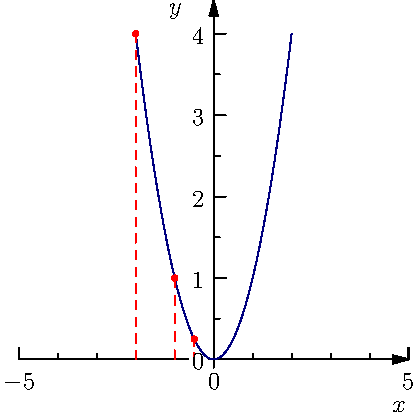
\includegraphics[width=0.5\linewidth]{images/image-1.pdf}
\caption{A mathematical valley minus a mathematical ant.\label{figure-math-valley}}
\end{figure}
\hypertarget{p-3}{}%
Remember that a function \(f\) of the variable \(x\) is just a rule that turns one number, \(x\), into another number, \(f(x)\). So the idea that the \emph{limit of a function} is trying to express is what happens to the number \(f(x)\) (the output) as the number \(x\) (the input) approaches some particular value.%
\begin{aside}{}{aside-1}%
\hypertarget{p-4}{}%
Actually, functions are much more general than this. But for calculus, it won't hurt us to view functions in this way.%
\end{aside}
\hypertarget{p-5}{}%
We're not quite ready to define the limit of a function precisely, but we can point one thing out right away: \emph{the limit of a function requires two pieces of information: the function itself and the number that \(x\) is approaching.} The limit should then be whatever number that \(f(x)\) is approaching.%
\begin{example}{Estimating the limit of a trigonometric function.}{example-estimating-the-limit-of-a-trigonometric-function}%
\hypertarget{p-6}{}%
Let \(f(x) = \sin x\cos x\). What is the limit of \(f(x)\) as \(x\) approaches the number \(\pi\)?%
\par\smallskip%
\noindent\textbf{Solution}.\hypertarget{solution-1}{}\quad%
\hypertarget{p-7}{}%
We don't have a lot of tools to find limits yet, so we'll try to estimate it instead. What we'll do is we'll plug numbers that are closer and closer to \(\pi\) into \(f(x)\). Let's list several values of \(f(x)\) as \(x\) gets closer to \(\pi\) from the left:%
\begin{table}
\centering
\begin{tabular}{cc}\hrulethick
\(x\)&\(f(x)\)\tabularnewline\hrulethin
\(3\)&\(-.140\)\tabularnewline[0pt]
\(3.1\)&\(-.042\)\tabularnewline[0pt]
\(3.14\)&\(-.002\)\tabularnewline\hrulethick
\end{tabular}
\end{table}
\hypertarget{p-8}{}%
We can even let \(x\) approach \(\pi\) from the other direction as well (i.e. "from the right") and \(f(x)\) will still approach \(0\) as \(x\) gets closer and closer to \(\pi\). So it looks like the limit should be \(0\).%
\end{example}
\hypertarget{p-9}{}%
To keep ourselves from writing "the limit of \(f(x)\) as \(x\) approaches some number \(a\)" over and over, let's introduce some notation: \(\lim_{x\to a}f(x)\).%
\begin{example}{Limit of a piecewise function.}{example-limit-of-a-piecewise-function}%
\hypertarget{p-10}{}%
Let%
%
\begin{equation*}
f(x) = \begin{cases} \sin x & \text{if $x<0$} \\ \cos x & \text{otherwise} \end{cases}.
\end{equation*}
\hypertarget{p-11}{}%
Find \(\lim_{x\to0}f(x)\).%
\par\smallskip%
\noindent\textbf{Solution}.\hypertarget{solution-2}{}\quad%
\hypertarget{p-12}{}%
If we graph this function, we see that at \(x=0\) there is a jump in the graph. In particular, if \(x\) approaches \(0\) from the left then \(f(x)\) approaches \(0\), whereas if \(x\) approaches \(0\) from the right then \(f(x)\) approaches \(1\). So this function does not appear to have an unambiguous limit as \(x\) approaches \(0\). Another way to say this: \(\lim_{x\to0}f(x)\) \emph{does not exist}.%
\end{example}
\hypertarget{p-13}{}%
\hyperref[example-limit-of-a-piecewise-function]{Example~\ref{example-limit-of-a-piecewise-function}} shows us something very important about limits: they depend on the two different ways \(x\) can approach a number. So we introduce two new pieces of notation: the \terminology{left-hand limit} \(\lim_{x\to a^{-}}f(x)\) will stand for the value \(f(x)\) approaches (if any) as \(x\) approaches \(a\) from the left (i.e. as \(x\) increases to \(a\)), and \terminology{the right-hand limit} \(\lim_{x\to a^{+}}f(x)\) will stand for the value \(f(x)\) approaches (if any) as \(x\) approaches \(a\) from the right (i.e. as \(x\) decreases to \(a\)).%
\par
\hypertarget{p-14}{}%
At this point, we can make a rough definition for the limit of a function.%
\begin{definition}{Limit of a Function.}{definition-limit-of-a-function}%
\index{limit!function of a single variable}\hypertarget{p-15}{}%
Let \(f(x)\) be a function. Suppose that both the left-hand limit \(\lim_{x\to a^{-}}f(x)\) and the right-hand limit \(\lim_{x\to a^{+}}f(x)\) exist and are equal to the same number \(L\). Then we say that the limit of \(f(x)\) as \(x\) approaches \(a\) exists and is equal to \(L\). We denote this by writing \(\lim_{x\to a}f(x) = L\).%
\end{definition}
\begin{example}{Piecewise function again.}{example-piecewise-function-again}%
\hypertarget{p-16}{}%
Let \(f(x)\) be given by%
\begin{equation*}
f(x) = \begin{cases} 0 & -3\leq x \leq -1 \\ x^{2} & -1 < x < \frac{1}{2} \\ \frac{1-x}{2} & \frac{1}{2} < x < 3. \end{cases} 
\end{equation*}
Evaluate \(\lim_{x\to-1}f(x)\) and \(\lim_{x\to\frac{1}{2}}f(x)\).%
\par\smallskip%
\noindent\textbf{Solution}.\hypertarget{solution-3}{}\quad%
\hypertarget{p-17}{}%
If we graph \(f(x)\), we get the following:%
\begin{figure}
\centering
{
\pgfmathdeclarefunction{MyFunction}{1}{%
  \pgfmathparse{%
    (and(   1,    #1<-1)*(0)            +%
    (and(#1>=-1,  #1< .5)*(#1*#1)   +%
    (and(#1>= .5,  #1< 3)*(.5-0.5*#1)%
    }%
}
\begin{tikzpicture}
    \begin{axis}[%
        axis x line = center,
        axis y line = center,
        xtick={-3,...,3},
        ytick={-3,...,3},
        xmin = -4,
        xmax = 4,
        ymin = -1.5,
        ymax = 1.5,
        xlabel={$x$},
        ylabel={$y$},
        grid=both
        ]
        \foreach \xStart/\xEnd  in {-3/-1, -1/.5, .5/3} {
        \addplot[domain=\xStart:\xEnd, blue, samples=10, ultra thick] {MyFunction(x)};
        }
        \addplot[incl] coordinates{(-3,0)};
        \addplot[incl] coordinates{(-1,0)};
        \addplot[excl] coordinates{(-1,1)};
        \addplot[excl] coordinates{(.5,.25)};
        \addplot[excl] coordinates{(3,-1)};
        \addlegendentry{$y = f(x)$};
    \end{axis}
\end{tikzpicture}
}
\end{figure}
\hypertarget{p-18}{}%
The graph shows us that \(\lim_{x\to-1^{-}}f(x) = 0\), while \(\lim_{x\to-1^{+}}f(x) = 1\). Therefore \(\lim_{x\to-1}f(x)\) does not exist. On the other hand, \(\lim_{x\to\frac{1}{2}}f(x)\) exists and is equal to \(\frac{1}{4}\).%
\end{example}
\end{subsectionptx}
\end{sectionptx}
%
%
\typeout{************************************************}
\typeout{Section 1.2 Computing Limits}
\typeout{************************************************}
%
\begin{sectionptx}{Computing Limits}{}{Computing Limits}{}{}\label{section-computing-limits}
\begin{introduction}{}%
\hypertarget{p-19}{}%
We've got a handle on how to estimate limits from \hyperref[section-the-limit-of-a-function]{Section~\ref{section-the-limit-of-a-function}}, but the process is very tedious. It requires either graphing the function in question or laboriously entering values into a calculator. So our first order of business now that we have the concept of a limit is to find an easier way to calculate it. This will be a running theme throughout the course.%
\end{introduction}%
%
%
\typeout{************************************************}
\typeout{Subsection 1.2.1 The Limit Laws}
\typeout{************************************************}
%
\begin{subsectionptx}{The Limit Laws}{}{The Limit Laws}{}{}\label{subsection-the-limit-laws}
\hypertarget{p-20}{}%
In many cases of interest, we can use knowledge of simpler limits to obtain more complicated limits. We do this via the \terminology{Limit Laws}. Before we get to them, we'll state two very simple (and hopefully very believable) limits.%
\begin{proposition}{Simple Limits.}{}{proposition-simple-limits}%
\hypertarget{p-21}{}%
For any value of \(a\), the following limits hold:%
\begin{equation*}
\lim_{x\to a}c = c
\end{equation*}
if \(c\) is a constant and%
\begin{equation*}
\lim_{x\to a}x = a.
\end{equation*}
%
\end{proposition}
\begin{theorem}{The Limit Laws.}{}{theorem-the-limit-laws}%
\hypertarget{p-22}{}%
Let \(c\) be a constant, let \(n\) be a positive whole number and let \(f(x)\) and \(g(x)\) be functions. Suppose that \(\lim_{x\to a}f(x)\) and \(\lim_{x\to a}g(x)\) both exist for some number \(a\). Then the following rules hold:%
\begin{table}
\centering
\begin{tabular}{ll}\hrulethick
\(1. \lim_{x\to a}[f(x)\pm g(x)] = \lim_{x\to a}f(x)\pm \lim_{x\to a}g(x)\)&\(2. \lim_{x\to a}cf(x) = c\lim_{x\to a}f(x)\)\tabularnewline[0pt]
\(3. \lim_{x\to a}[f(x)g(x)] = \lim_{x\to a}f(x)\lim_{x\to a}g(x)\)&\(4. \lim_{x\to a}\frac{f(x)}{g(x)} = \frac{\lim_{x\to a}f(x)}{\lim_{x\to a}g(x)}\) (if \(\lim_{x\to a}g(x)\neq 0\))\tabularnewline[0pt]
\(5. \lim_{x\to a}[f(x)^{n}] = [\lim_{x\to a}f(x)]^{n}\)&\(6. \lim_{x\to a}\sqrt[n]{f(x)} = \sqrt[n]{\lim_{x\to a}f(x)}\)\tabularnewline\hrulethick
\end{tabular}
\caption{The Limit Laws.\label{table-limit-laws}}
\end{table}
\hypertarget{p-23}{}%
Note that item six in the table above only holds (in this class...) if \(n\) is odd or if \(\lim_{x\to a}f(x)\geq0\).%
\end{theorem}
\hypertarget{p-24}{}%
\hyperref[theorem-the-limit-laws]{Theorem~\ref{theorem-the-limit-laws}} gives us the ability to compute a wide variety of limits.%
\begin{example}{Limit of a rational function.}{example-limit-of-a-rational-function}%
\hypertarget{p-25}{}%
Let%
\begin{equation*}
f(x) = \frac{3 - x^{5} + 5x}{2x-\sqrt[4]{x}}.
\end{equation*}
Evaluate \(\lim_{x\to 16}f(x)\).%
\par\smallskip%
\noindent\textbf{Solution}.\hypertarget{solution-4}{}\quad%
\hypertarget{p-26}{}%
We can evaluate \(\lim_{x\to 16}f(x)\) by making use of the appropriate Limit Laws and \hyperref[proposition-simple-limits]{Proposition~\ref{proposition-simple-limits}}:%
%
\begin{align*}
\lim_{x\to 16}\frac{3 - x^{5} + 5x}{2x-\sqrt[4]{x}} & = \frac{\lim_{x\to 16}(3 - x^{5} + 5x)}{\lim_{x\to 16}(2x-\sqrt[4]{x})} & \text{by Limit Law 4}\\
& = \frac{\lim_{x\to 16}3 - \lim_{x\to 16}x^{5} + \lim_{x\to 16}5x}{\lim_{x\to 16}2x-\lim_{x\to 16}\sqrt[4]{x}} & \text{by Limit Law 1.} \\
& = \frac{3 - [\lim_{x\to 16}x]^{5} + 5\lim_{x\to 16}x}{2\lim_{x\to 16}x-\sqrt[4]{\lim_{x\to 16}x}} & \text{by Limit Laws 2, 5, and 6.} \\
& = \frac{3-16^{5}+80}{30} &
\end{align*}
\end{example}
\hypertarget{p-27}{}%
In particular, Limit Laws 1-5 give us the following: if \(f(x)\) is a polynomial or rational function, then \(\lim_{x\to a}f(x) = f(a)\) as long as \(a\) is in the domain of \(f(x)\). If \(a\) is not in the domain, trickery may be required.%
\begin{example}{Trickery.}{example-trickery}%
\hypertarget{p-28}{}%
Evaluate%
\begin{equation*}
\lim_{x\to1}\frac{\sqrt{x}-1}{x-1}.
\end{equation*}
%
\par\smallskip%
\noindent\textbf{Solution}.\hypertarget{solution-5}{}\quad%
\hypertarget{p-29}{}%
First, note that we can't use the Limit Laws right away since the denominator is \(0\) at \(x=1\). What we need to do is use algebra to simplify the expression inside the limit:%
%
\begin{align*}
\frac{\sqrt{x}-1}{x-1} & = \frac{\sqrt{x}-1}{x-1}\frac{\sqrt{x}+1}{\sqrt{x}+1} \\
& = \frac{x - 1}{(x-1)(\sqrt{x}+1)} \\
& = \frac{1}{\sqrt{x}+1}. 
\end{align*}
\hypertarget{p-30}{}%
Now we can use the Limit Laws to find the limit as \(x\) approaches \(1\), since we no longer have a divide-by-zero problem in the denominator:%
%
\begin{align*}
\lim_{x\to1}\frac{\sqrt{x}-1}{x-1} & = \lim_{x\to1}\frac{1}{\sqrt{x}+1} \\
& = \frac{1}{2}. 
\end{align*}
\end{example}
\end{subsectionptx}
\end{sectionptx}
%
%
\typeout{************************************************}
\typeout{Section 1.3 Continuity}
\typeout{************************************************}
%
\begin{sectionptx}{Continuity}{}{Continuity}{}{}\label{section-continuity}
\hypertarget{p-31}{}%
We saw in \hyperref[section-computing-limits]{Section~\ref{section-computing-limits}} that for a function like \(f(x) = x+3x^{2}\), we could evaluate \(\lim_{x\to a}f(x)\) by simply plugging in \(x=a\). In other words, \(\lim_{x\to a}f(x) = f(a)\). Functions that have this property are extremely important in mathematics, so we give them a name.%
\begin{definition}{Continuous Functions.}{definition-continuous-functions}%
\index{continuous functions!definition}\hypertarget{p-32}{}%
Let \(f(x)\) be a function and suppose that \(a\) is in the domain of \(f(x)\). Then we say that \(f(x)\) is \terminology{continuous at \(a\)} if%
\begin{equation*}
\lim_{x\to a}f(x) = f(a)\text{.}
\end{equation*}
Otherwise, we say that \(f(x)\) is \terminology{discontinuous at \(a\)}. We say that \(f(x)\) is continuous on an interval if it is continuous at every point of an interval. Otherwise, we say that \(f(x)\) is discontinuous on the interval.%
\end{definition}
\hypertarget{p-33}{}%
\hyperref[definition-continuous-functions]{Definition~\ref{definition-continuous-functions}} says that it is extremely easy to evaluate limits of continuous functions: just plug the value that \(x\) is approaching into the function \(f(x)\). So the limit is then \(f(a)\). If a function \(f(x)\) is continuous on an interval, then this means that the graph of \(f(x)\) has no "gaps" over this interval.%
\begin{example}{Determining if a function is continuous.}{example-determining-if-a-function-is-continuous}%
\hypertarget{p-34}{}%
Let \(f(x) = \frac{1}{x}\). Is \(f(x)\) continuous on \((-\infty,\infty)\)?%
\par\smallskip%
\noindent\textbf{Solution}.\hypertarget{solution-6}{}\quad%
\hypertarget{p-35}{}%
If we graph \(f(x)\), then we see that it is discontinuous at \(x=0\). Therefore \(f(x)\) is discontinuous on the interval \((-\infty,\infty)\).%
\end{example}
\hypertarget{p-36}{}%
If we're dealing with a function on a (bounded) closed interval, we need to introduce some new terminology. We say that a function \(f(x)\) is \terminology{continuous from the left} at \(x=a\) if \(\lim_{x\to a^{-}}f(x) = f(a)\). Similarly, we say that \(f(x)\) is \terminology{continuous from the right} at \(x=a\) if \(\lim_{x\to a^{+}}f(x) = f(a)\). This is of course assuming that \(a\) is in the domain of \(f(x)\). Finally, we say that \(f(x)\) is continuous on the closed interval \([a,b]\) if it is continuous on \((a,b)\), continuous from the right at \(a\) and continuous from the left at \(b\). The main idea is still that the graph contains no gaps over this interval.%
\begin{example}{Continuity over a closed interval.}{example-continuity-over-a-closed-interval}%
\hypertarget{p-37}{}%
Let \(f(x)\) be given by%
\begin{equation*}
f(x) = \begin{cases} 3x-1 & 1\leq x< 2 \\ 9-x^{2} & 2\leq x\leq 4.\end{cases}
\end{equation*}
Is \(f(x)\) continuous over \([1,4]\)?%
\par\smallskip%
\noindent\textbf{Solution}.\hypertarget{solution-7}{}\quad%
\hypertarget{p-38}{}%
If we graph \(f(x)\) over this interval, we get the following:%
\begin{figure}
\centering
{
\pgfmathdeclarefunction{MyFunction}{1}{%
  \pgfmathparse{%
    (and(#1>=1,  #1< 2)*(3*#1-1)   +%
    (and(#1>= 2,  #1<= 4)*(9-#1*#1)%
    }%
}
\begin{tikzpicture}
    \begin{axis}[%
        axis x line = center,
        axis y line = center,
        xtick={0,...,5},
        ytick={-7,...,5},
        xmin = -1,
        xmax = 5,
        ymin = -7.5,
        ymax = 5.5,
        xlabel={$x$},
        ylabel={$y$},
        grid=both
        ]
        \foreach \xStart/\xEnd  in {1/2, 2/4} {
        \addplot[domain=\xStart:\xEnd, blue, samples=10, ultra thick] {MyFunction(x)};
        }
        \addplot[incl] coordinates{(1,2)};
        \addplot[incl] coordinates{(4,-7)};
        \addlegendentry{$y = f(x)$};
    \end{axis}
\end{tikzpicture}
}
\end{figure}
\hypertarget{p-39}{}%
So from the graph it appears that \(f(x)\) is continuous on this interval.%
\end{example}
\hypertarget{p-40}{}%
Remember that we said a function is continuous over an interval if its graph has no gaps over that interval. This is a very rough explanation of continuity, but it should make the following theorem plausible.%
\begin{theorem}{Continuous Functions.}{}{theorem-continuous-functions}%
\hypertarget{p-41}{}%
Polynomial, rational, root and trigonometric functions are continuous at every point of their domain.%
\end{theorem}
\hypertarget{p-42}{}%
Although it doesn't directly mention piecewise functions, \hyperref[theorem-continuous-functions]{Theorem~\ref{theorem-continuous-functions}} is still useful for determining if they are continuous. If a piecewise function is defined using any of the functions from \hyperref[theorem-continuous-functions]{Theorem~\ref{theorem-continuous-functions}}, then the only points we really need to check for continuity are the the places where the function "changes rules".%
\begin{example}{Another piecewise function.}{example-another-piecewise-function}%
\hypertarget{p-43}{}%
Over what intervals is the function \(g(s)\) given by%
\begin{equation*}
g(s) = \begin{cases} s^{2} & s<-1 \\ -5\cos (\pi s) & -1\leq s\leq 1 \\ 5 & s> 1 \end{cases}
\end{equation*}
continuous?%
\par\smallskip%
\noindent\textbf{Solution}.\hypertarget{solution-8}{}\quad%
\hypertarget{p-44}{}%
We need to check continuity at \(s=-1\) and \(s=1\). At \(s=-1\), we need to make sure that \(\lim_{s\to -1}g(s)\) exists and is equal to \(g(-1)\). Since%
\begin{equation*}
\lim_{s\to-1^{-1}}g(s) = \lim_{s\to-1^{-1}}s^{2} = 1
\end{equation*}
and%
\begin{equation*}
\lim_{s\to-1^{+}}g(s) = \lim_{s\to-1^{+}}\cos(\pi s) = -1,
\end{equation*}
it follows that \(\lim_{s\to-1}g(s)\) does not exist. So \(g(s)\) can't be continuous at \(s=-1\).%
\par
\hypertarget{p-45}{}%
On the other hand, since \(\lim_{s\to1^{-1}}g(s) = 5 = \lim_{s\to1^{+}}g(s)\), it follows that \(\lim_{s\to1}g(s)\) exists and is equal to \(5\). Since \(g(1)\) also equals \(5\), \(g(s)\) is continuous at \(s=1\). So \(g(s)\) must be continuous on \((-\infty, -1)\cup(-1,\infty)\).%
\end{example}
\hypertarget{p-46}{}%
We can also build more complicated continuous functions out of simpler ones.%
\begin{theorem}{Combining Continuous Functions.}{}{theorem-combining-continuous-functions}%
\hypertarget{p-47}{}%
Let \(f(x)\) and \(g(x)\) be continuous at a point \(a\). Then the following statements are true: \leavevmode%
\begin{enumerate}
\item\hypertarget{li-1}{}\(f(x)+g(x)\) is continuous at \(a\).%
\item\hypertarget{li-2}{}\(f(x)g(x)\) is continuous at \(a\).%
\item\hypertarget{li-3}{}\(\frac{f(x)}{g(x)}\) is continuous at \(a\) if \(g(a)\neq0\).%
\item\hypertarget{li-4}{}\(f(g(x))\) is continuous at \(a\) if \(g(a)\) is in the domain of \(f(x)\).%
\end{enumerate}
%
\end{theorem}
\begin{example}{Determining where functions are continuous.}{example-determining-where-functions-are-continuous}%
\hypertarget{p-48}{}%
Let \(h(t) = \sqrt{t} + \frac{t}{t-4} - \frac{t+1}{t^{2}-1}\). On what intervals is \(h(t)\) continuous?%
\par\smallskip%
\noindent\textbf{Solution}.\hypertarget{solution-9}{}\quad%
\hypertarget{p-49}{}%
By \hyperref[theorem-combining-continuous-functions]{Theorem~\ref{theorem-combining-continuous-functions}}, \(h(t)\) should be continuous wherever \(\sqrt{t}, \frac{t}{t-4}\) and \(\frac{t+1}{t^{2}-1}\) are all defined. Since \(\sqrt{t}\) is defined for \(t\geq0\), \(\frac{t}{t-4}\) is defined for \(t\neq4\) and \(\frac{t+1}{t^{2}-1}\) is defined for \(t\neq\pm1\), it follows that \(h(t)\) is continuous on \([0,1)\cup(1,4)\cup(4,\infty)\).%
\end{example}
\begin{example}{Using continuity to evaluate a limit.}{example-using-continuity-to-evaluate-a-limit}%
\hypertarget{p-50}{}%
Evaluate \(\lim_{x\to\pi}\cos(x+\sin x)\).%
\par\smallskip%
\noindent\textbf{Solution}.\hypertarget{solution-10}{}\quad%
\hypertarget{p-51}{}%
Since \(x, \cos x\) and \(\sin x\) are all continuous, this means that \(\cos(x+\sin x)\) must be continuous as well. Therefore%
\begin{equation*}
\lim_{x\to\pi}\cos(x+\sin x) = \cos(\pi+\sin\pi) = -1.
\end{equation*}
%
\end{example}
\end{sectionptx}
%
%
\typeout{************************************************}
\typeout{Section 1.4 Limits Involving Infinity}
\typeout{************************************************}
%
\begin{sectionptx}{Limits Involving Infinity}{}{Limits Involving Infinity}{}{}\label{section-limits-involving-infinity}
%
%
\typeout{************************************************}
\typeout{Subsection 1.4.1 Limits Involving Vertical Asymptotes}
\typeout{************************************************}
%
\begin{subsectionptx}{Limits Involving Vertical Asymptotes}{}{Limits Involving Vertical Asymptotes}{}{}\label{subsection-limits-involving-vertical-asymptotes}
\hypertarget{p-52}{}%
Consider the function \(f(x)=\frac{1}{x}\). We know from algebra that this function has a vertical asymptote at \(x=0\), and so in particular is undefined there. However, just because it's undefined at \(x=0\) doesn't mean that we can't gather important information about the function near \(0\). This is because the function behaves in a very specific way as we let \(x\) approach \(0\). For example, if we let \(x\) approach \(0\) from the right, then \(f(x)\) increases without bound. Similarly, \(f(x)\) decreases without bound as \(x\) approaches \(0\) from the left.%
\par
\hypertarget{p-53}{}%
Even though \(f(x)\) is not approaching a specific value as \(x\) approaches \(0\) from either direction, this behavior shows up often enough and is important enough that we want to introduce notation to describe it. For this function, we would say \(\lim_{x\to0^{+}}\frac{1}{x}=\infty\) and \(\lim_{x\to0^{-}}\frac{1}{x}=-\infty\).%
\par
\hypertarget{p-54}{}%
Now consider \(g(x) = \frac{1}{(x-3)^{2}}\). Then \(\lim_{x\to3^{-}}g(x) = \lim_{x\to3^{+}}g(x) = \infty\) since the function increases without bound when \(x\) approaches \(3\) from both directions. In this case, we say that \(\lim_{x\to3}g(x)=\infty\).%
\begin{aside}{}{aside-2}%
\hypertarget{p-55}{}%
It's \emph{extremely} important to remember that the symbol \(\infty\) is not being used to represent a number or variable that we can perform algebra on. It's a symbol indicating how a particular function is behaving at a certain point.%
\end{aside}
\hypertarget{p-56}{}%
If \(f(x)\) is a function and \(\lim_{x\to a}f(x)=\pm\infty\), \(\lim_{x\to a^{-}}f(x)=\pm\infty\) or \(\lim_{x\to a^{+}}f(x)=\pm\infty\), then this means that the function has a vertical asymptote at \(x=a\). In this course, this basically corresponds to a divide-by-zero problem.%
\begin{example}{Infinite limit involving a rational function.}{example-infinite-limit-involving-a-rational-function}%
\hypertarget{p-57}{}%
Determine \(\lim_{x\to4^{-}}\frac{x-3}{2x-8}\).%
\par\smallskip%
\noindent\textbf{Solution}.\hypertarget{solution-11}{}\quad%
\hypertarget{p-58}{}%
If we try to plug in \(x=4\) into \(\frac{x-3}{2x-8}\) we get \(\frac{1}{0}\), which means we have run into a divide-by-zero problem. This is a good hint that the limit should be \(\pm\infty\), we just need to figure out the correct sign. There are a couple ways we can do this. First, we could set up a sign chart for this function to see where it's positive and negative and then use that to see if it's increasing or decreasing without bound as \(x\to4^{-}\). Second, we could just plug in values of \(x\) that are closer and closer to \(4\) and see how the function behaves. Either way, we see that it's negative for values of \(x\) that are close to (but less than) \(4\). Hence \(\lim_{x\to4^{-}}\frac{x-3}{2x-8}=-\infty\).%
\end{example}
\end{subsectionptx}
%
%
\typeout{************************************************}
\typeout{Subsection 1.4.2 Limits at Infinity}
\typeout{************************************************}
%
\begin{subsectionptx}{Limits at Infinity}{}{Limits at Infinity}{}{}\label{subsection-limits-at-infinity}
\hypertarget{p-59}{}%
\hyperref[subsection-limits-involving-vertical-asymptotes]{Subsection~\ref{subsection-limits-involving-vertical-asymptotes}} involved limits of functions whose values approached \(\pm\infty\). Now we look at what can happen to a function if its input values approach \(\pm\infty\). First, a definition of sorts.%
\begin{definition}{Limit at Infinity.}{definition-limit-at-infinity}%
\hypertarget{p-60}{}%
Let \(f(x)\) be a function. We say that \(\lim_{x\to\infty}f(x) = L\) if \(f(x)\) gets (and stays) arbitrarily close to \(L\) as \(x\) is made arbitrarily large. Similarly, we say that \(\lim_{x\to-\infty}f(x) = L\) if \(f(x)\) gets (and stays) arbitrarily close to \(L\) as \(x\) is made arbitrarily small.%
\end{definition}
\begin{example}{An important limit at infinity.}{example-an-important-limit-at-infinity}%
\hypertarget{p-61}{}%
Let \(f(x) = \frac{1}{x}\). Determine \(\lim_{x\to\infty}f(x)\).%
\par\smallskip%
\noindent\textbf{Solution}.\hypertarget{solution-12}{}\quad%
\hypertarget{p-62}{}%
As \(x\) gets arbitrarily large, \(\frac{1}{x}\) gets arbitrarily close to \(0\). Therefore \(\lim_{x\to\infty}f(x) = 0\).%
\end{example}
\hypertarget{p-63}{}%
\hyperref[example-an-important-limit-at-infinity]{Example~\ref{example-an-important-limit-at-infinity}} holds for many other reciprocal powers of \(x\). In particular, if \(n>0\) then \(\lim_{x\to\infty}\frac{1}{x^{n}} = \lim_{x\to-\infty}\frac{1}{x^{n}} = 0\).%
\begin{example}{A limit at infinity involving cosine.}{example-a-limit-at-infinity-involving-sine}%
\hypertarget{p-64}{}%
Let \(g(s) = \cos s^{-3}\). Compute \(\lim_{s\to-\infty}g(s)\).%
\par\smallskip%
\noindent\textbf{Solution}.\hypertarget{solution-13}{}\quad%
\hypertarget{p-65}{}%
First, note that \(g(s) = \cos\frac{1}{s^{3}}\). By the previous remark, we know that \(\lim_{s\to-\infty}\frac{1}{s^{3}} = 0\). Therefore \(\lim_{s\to-\infty}g(s) = \cos0 = 1\).%
\end{example}
\begin{aside}{}{aside-3}%
\hypertarget{p-66}{}%
The reason we were able to find the limit in \hyperref[example-a-limit-at-infinity-involving-sine]{Example~\ref{example-a-limit-at-infinity-involving-sine}} was because of the following fact: if \(\lim_{x\to a}g(x)\) exists and if \(f(x)\) is continuous at \(\lim_{x\to a}g(x)\), then \(\lim_{x\to a}f(g(x)) = f(\lim_{x\to a}g(x))\). Basically, we can swap continuous functions with limits without causing any harm.%
\end{aside}
\hypertarget{p-67}{}%
For limits at infinity involving powers of a variable, it is the highest power variables that determine the outcome.%
\begin{example}{Limit at infinity of a rational function.}{example-limit-at-infinity-of-a-rational-function}%
\hypertarget{p-68}{}%
Let%
\begin{equation*}
f(t) = \frac{100t - 3 + t^{3}}{5t^{2}+1}\text{ and } g(t) = \frac{1-2t^{4}}{5t^{4}+3000t}.
\end{equation*}
Find \(\lim_{t\to\infty} f(t)\) and \(\lim_{t\to-\infty}g(t)\).%
\par\smallskip%
\noindent\textbf{Solution}.\hypertarget{solution-14}{}\quad%
\hypertarget{p-69}{}%
Let's start with \(f(t)\). To figure out what this limit should be, we could try the following. As \(t\) gets very large the \(t^{3}\) term in the numerator should drown out everything else in the numerator. Similarly, the \(5t^{2}\) term in the denominator should drown out everything else in the denominator. So for \(t\) very large, \(f(t)\approx\frac{t^{3}}{5t^{2}} = \frac{1}{5}t\). Hence \(f(t)\) should probably go to \(\infty\) as \(t\) goes to \(\infty\). To make this more precise, we'll just divide the numerator and denominator by the largest power of the denominator, \(t^{2}\), and then take the limit:%
%
\begin{align*}
\lim_{t\to\infty}f(t) & = \lim_{t\to\infty}\frac{100t-3+t^{3}}{5t^{2}+1} \\
& = \lim_{t\to\infty}\frac{\frac{100}{t} - \frac{3}{t^{2}}+t}{5+\frac{1}{t^{2}}} \\
& = \infty. 
\end{align*}
\hypertarget{p-70}{}%
We can find \(\lim_{t\to-\infty}g(t)\) using the same idea. Just divide by the highest power in the denominator and then take the limit:%
%
\begin{align*}
\lim_{t\to-\infty}g(t) & = \lim_{t\to-\infty}\frac{\frac{1}{t^{4}}-2}{5+\frac{3000}{t^{3}}} \\
& = -\frac{2}{5}. 
\end{align*}
\end{example}
\hypertarget{p-71}{}%
These limits at infinity have a graphical meaning as well. If \(\lim_{x\to\infty}f(x)\) or \(\lim_{x\to-\infty}f(x)\) exists and is equal to \(L\), then the line \(y=L\) is a horizontal asymptote of the graph of \(y=f(x)\).%
\begin{example}{Asymptotic equivalence.}{example-asymptotic-equivalence}%
\hypertarget{p-72}{}%
Two functions \(f(x)\) and \(g(x)\) are said to be \terminology{asymptotically equivalent}, written \(f\sim g\), if the following is true:%
\begin{equation*}
\lim_{x\to\infty}\frac{f(x)}{g(x)} = 1.
\end{equation*}
Show that \(\sin\frac{1}{x}\sim\frac{1}{x}\).%
\par\smallskip%
\noindent\textbf{Solution}.\hypertarget{solution-15}{}\quad%
\hypertarget{p-73}{}%
All we need to do is compute \(\lim_{x\to\infty}\frac{\sin\frac{1}{x}}{\frac{1}{x}}:\)%
\begin{align*}
\lim_{x\to\infty}\frac{\sin\frac{1}{x}}{\frac{1}{x}} & = \lim_{\theta\to0^{+}}\frac{\sin\theta}{\theta} \\
& = 1. 
\end{align*}
Therefore \(\sin\frac{1}{x}\sim\frac{1}{x}\).%
\end{example}
\end{subsectionptx}
\end{sectionptx}
\end{chapterptx}
%
%
\typeout{************************************************}
\typeout{Chapter 2 Derivatives}
\typeout{************************************************}
%
\begin{chapterptx}{Derivatives}{}{Derivatives}{}{}\label{derivatives}
\begin{introduction}{}%
\hypertarget{p-74}{}%
There are two problems that inspired the creation of calculus. The first is the tangent line problem, or rate of change problem. This problem is concerned with determining how a quantity \(f(x)\) changes as \(x\) varies. We will focus on this problem and its solution, derivatives, for the next two chapters. Afterwards, we will focus on the area problem, the second problem that inspired the creation of calculus.%
\end{introduction}%
%
%
\typeout{************************************************}
\typeout{Section 2.1 The Definition of the Derivative}
\typeout{************************************************}
%
\begin{sectionptx}{The Definition of the Derivative}{}{The Definition of the Derivative}{}{}\label{section-the-definition-of-the-derivative}
%
%
\typeout{************************************************}
\typeout{Subsection 2.1.1 Tangent Lines}
\typeout{************************************************}
%
\begin{subsectionptx}{Tangent Lines}{}{Tangent Lines}{}{}\label{subsection-tangent-lines}
\hypertarget{p-75}{}%
Consider \(f(x) = x^{2}\). If we graph this, we get a parabola. What we'd like to do is to find a way to describe how quickly this parabola is changing at a point, i.e. find the "slope" of the parabola. One way to try to deal with this is to use \terminology{secant lines}. Recall that the secant line through the points \((a,f(a))\) and \((b,f(b))\) has slope \(\frac{f(b) - f(a)}{b-a}\), which is just the average rate of change of \(f\) from \(x=a\) to \(x=b\). If \(b\) is very close to \(a\), then the slope of the secant line through these points should be a good approximation to the "slope" of \(f(x) = x^{2}\) at the point \(x=a\).%
\begin{example}{Secant lines on a parabola.}{example-secant-lines-on-a-parabola}%
\hypertarget{p-76}{}%
Let \(f(x) = x^{2}\). Find the slope of the secant line through \((2,f(2))\) and \((x,f(x))\).%
\par\smallskip%
\noindent\textbf{Solution}.\hypertarget{solution-16}{}\quad%
\hypertarget{p-77}{}%
Since the slope of the secant line is the average rate of change, we get that the slope must be equal to%
\begin{equation*}
\frac{f(x) - f(2)}{x-2} = \frac{x^{2} - 4}{x-2} = x+2.
\end{equation*}
%
\end{example}
\hypertarget{p-78}{}%
What \hyperref[example-secant-lines-on-a-parabola]{Example~\ref{example-secant-lines-on-a-parabola}} is telling us is that if \(x\approx2\), then the slope of \(f(x) = x^{2}\) at \(x=2\) should be very close to \(x+2\), the slope of the secant line. Now we'll do a trick that shows up everywhere in calculus, and is the entire reason we introduced limits in the first place. We'll make this approximation exact by taking a limit. In particular, we'll say that the slope of \(f(x) = x^{2}\) should be equal to%
\begin{equation*}
\lim_{x\to2}\frac{f(x)-f(2)}{x-2} = \lim_{x\to2}(x+2) = 4.
\end{equation*}
This is the slope of the \terminology{tangent line} to \(f(x) = x^{2}\) at \(x=2\). Instead of an average rate of change over an interval \([2,x]\), we now have an \terminology{instantaneous rate of change} at a point \(x=2\).%
\begin{definition}{Tangent Lines.}{definition-tangent-lines}%
\hypertarget{p-79}{}%
The tangent line to a curve \(y=f(x)\) through a point \((a,f(a))\) is the line passing through \((a,f(a))\) with slope given by%
\begin{equation*}
\lim_{x\to a}\frac{f(x)-f(a)}{x-a},
\end{equation*}
assuming this limit exists. The slope of the tangent line represents the slope of the graph of \(f(x)\) at \(a\) and gives the instantaneous rate of change of \(f(x)\) at \(x=a\).%
\end{definition}
\begin{example}{Tangent line to a root.}{example-tangent-line-to-a-root}%
\hypertarget{p-80}{}%
Find the equation of the tangent line to \(y=\sqrt{x}\) through the point \((4,2)\).%
\par\smallskip%
\noindent\textbf{Solution}.\hypertarget{solution-17}{}\quad%
\hypertarget{p-81}{}%
We need two things to find the equation of a line: the slope of the line and a point on the line. Since we know the tangent line has to pass through \((4,2)\), we just need to find the slope. The slope is given by%
\begin{equation*}
\lim_{x\to 4}\frac{\sqrt{x}-2}{x-4} = \lim_{x\to4}\frac{x-4}{(x-4)(\sqrt{x}+2)} = \frac{1}{4}.
\end{equation*}
Hence the equation of the tangent line through \((4,2)\) is%
\begin{equation*}
y-2 = \frac{1}{4}(x-4).
\end{equation*}
%
\end{example}
\hypertarget{p-82}{}%
As a reminder, the slope of the tangent line represents the slope, or instantaneous rate of change, of the function.%
\begin{example}{Velocity from position.}{example-velocity-from-position}%
\hypertarget{p-83}{}%
The displacement (i.e. position) of a particle moving in a straight line is described by the function \(s(t) = 3t^{2} - 5t\), where \(t\) is in seconds and \(s\) is in meters. Find the velocity, or instantaneous rate of change, of the particle at \(t=3\).%
\par\smallskip%
\noindent\textbf{Solution}.\hypertarget{solution-18}{}\quad%
\hypertarget{p-84}{}%
The velocity is just the slope of the tangent line to \(s(t)\) at \(t=3\), which we can find as follows:%
%
\begin{align*}
\lim_{t\to3}\frac{s(t) - s(3)}{t-3} & = \lim_{t\to3}\frac{(3t^{2} - 5t) - 12}{t-3} \\
& = \lim_{t\to3}\frac{3t^{2} - 5t - 12}{t-3} 
\end{align*}
\hypertarget{p-85}{}%
At this step it's a little unclear where to go next, so we'll try long division. If we do so, we get%
\begin{equation*}
\frac{3t^{2} - 5t - 12}{t-3} = 3t+4.
\end{equation*}
Hence the velocity must be%
\begin{equation*}
\lim_{t\to3}(3t+4) = 13
\end{equation*}
meters per second.%
\end{example}
\hypertarget{p-86}{}%
\hyperref[example-velocity-from-position]{Example~\ref{example-velocity-from-position}} was a little tricky because we needed to compute \(\lim_{t\to3}\frac{3t^{2}-5t-12}{t-3}\), and it was unclear how to simplify this at first. This stemmed in large part from how we computed the velocity in the first place, using the formula%
\begin{equation*}
\lim_{t\to3}\frac{s(t)-s(3)}{t-3}
\end{equation*}
or more generally%
\begin{equation*}
\lim_{x\to a}\frac{f(x) - f(a)}{x-a}\text{.}
\end{equation*}
%
\par
\hypertarget{p-87}{}%
We want to rewrite this formula to make it a little easier to work with in certain cases. We'll do this by making the denominator easier to handle. In particular, set \(x-a = h\). Then%
\begin{equation*}
\lim_{x\to a}\frac{f(x) - f(a)}{x-a} = \lim_{h\to0}\frac{f(a+h)-f(a)}{h}.
\end{equation*}
Either formula can be used to compute the slope of the tangent line.%
\begin{example}{Velocity revisited.}{example-velocity-revisited}%
\hypertarget{p-88}{}%
Let \(s(t)\) be given as in \hyperref[example-velocity-from-position]{Example~\ref{example-velocity-from-position}}. Find the velocity at \(t=3\).%
\par\smallskip%
\noindent\textbf{Solution}.\hypertarget{solution-19}{}\quad%
\hypertarget{p-89}{}%
We know that the velocity should be \(13\), but we'll try to find it again using our new formula. So the velocity should also be%
%
\begin{align*}
\lim_{h\to0}\frac{s(3+h)-s(3)}{h} & = \lim_{h\to0}\frac{3(9+6h+h^{2})-5(3+h)-12}{h} \\
& = \lim_{h\to0}\frac{13h+3h^{2}}{h} \\
& = \lim_{h\to0}(13+3h) \\
& = 13. 
\end{align*}
\end{example}
\hypertarget{p-90}{}%
Typically, if \(f(x)-f(a)\) is easy to factor in terms of \(x-a\) we'll want to use the first formula we had for computing rates of change. Otherwise, we'll stick with the new formula involving \(h\).%
\end{subsectionptx}
%
%
\typeout{************************************************}
\typeout{Subsection 2.1.2 The Derivative}
\typeout{************************************************}
%
\begin{subsectionptx}{The Derivative}{}{The Derivative}{}{}\label{subsection-the-derivative}
\hypertarget{p-91}{}%
Suppose we go back to \hyperref[example-velocity-from-position]{Example~\ref{example-velocity-from-position}} one more time, but now we want to find the velocity of \(s(t)\) at an arbitrary number \(a\). Then we could still use our limit formulas, which would give us%
%
\begin{align*}
\lim_{h\to0}\frac{s(a+h)-s(a)}{h} & = \lim_{h\to0}\frac{3(a^{2}+2ah+h^{2})-5(a+h) - 3a^{2} + 5a}{h} \\
& = \lim_{h\to0}\frac{6ah+3h^{2} - 5h}{h} \\
& = \lim_{h\to0}(6a+3h-5) \\
& = 6a-5. 
\end{align*}
\hypertarget{p-92}{}%
So the velocity at \(t=a\) of the particle modeled by \(s(t)\) is given by \(6a-5\). So we can represent the velocity, or rate of change or slope of the tangent line, by a function. We call this the \terminology{derivative}.%
\begin{definition}{Definition of the Derivative.}{definition-definition-of-the-derivative}%
\index{derivative!definition}\index{functions!differentiable}\hypertarget{p-93}{}%
Let \(f(x)\) be a function. Then its derivative at \(x=a\) is the number \(f'(a)\) given by%
\begin{equation*}
f'(a) = \lim_{h\to0}\frac{f(a+h)-f(a)}{h}
\end{equation*}
assuming the limit exists. If this limit exists, we say that the function \(f(x)\) is \terminology{differentiable} at \(a\).%
\end{definition}
\begin{aside}{}{aside-4}%
\hypertarget{p-94}{}%
We could also define the derivative by%
\begin{equation*}
\lim_{x\to a}\frac{f(x)-f(a)}{x-a}.
\end{equation*}
These two limits are equivalent.%
\end{aside}
\hypertarget{p-95}{}%
The derivative of a function \(f(x)\) at a point \(a\) represents two things: the slope of the tangent line to \(f(x)\) at \(a\) and the instantaneous rate of change of \(f(x)\) at \(a\).%
\begin{example}{Slope of the sine function.}{example-slope-of-the-sine-function}%
\hypertarget{p-96}{}%
Let \(f(x) = \sin x\). Find its slope at \(0\).%
\par\smallskip%
\noindent\textbf{Solution}.\hypertarget{solution-20}{}\quad%
\hypertarget{p-97}{}%
The slope at \(0\) is exactly \(f'(0)\), which is%
\begin{equation*}
\lim_{h\to0}\frac{\sin(0+h)-\sin(0)}{h} = \lim_{h\to0}\frac{\sin h}{h} = 1.
\end{equation*}
%
\end{example}
\begin{example}{Tangent line of the sine function.}{example-tangent-line-of-the-sine-function}%
\hypertarget{p-98}{}%
Find the equation of the tangent line to \(f(x) = \sin x\) at \(0\).%
\par\smallskip%
\noindent\textbf{Solution}.\hypertarget{solution-21}{}\quad%
\hypertarget{p-99}{}%
The tangent line must pass through \((0,0)\) and must have slope \(f'(0) = 1\), so its equation is%
\begin{equation*}
y-0 = 1(x-0)
\end{equation*}
or just \(y=x\).%
\end{example}
\end{subsectionptx}
\end{sectionptx}
%
%
\typeout{************************************************}
\typeout{Section 2.2 The Derivative as a Function}
\typeout{************************************************}
%
\begin{sectionptx}{The Derivative as a Function}{}{The Derivative as a Function}{}{}\label{section-the-derivative-as-a-function}
%
%
\typeout{************************************************}
\typeout{Subsection 2.2.1 The Derivative Function}
\typeout{************************************************}
%
\begin{subsectionptx}{The Derivative Function}{}{The Derivative Function}{}{}\label{subsection-the-derivative-function}
\hypertarget{p-100}{}%
There's no reason we can't look at an arbitrary value for \(a\) in the definition of \(f'(a)\) given in \hyperref[definition-definition-of-the-derivative]{Definition~\ref{definition-definition-of-the-derivative}}. If we do this, we can define the \emph{derivative function}.%
\begin{definition}{The Derivative Function.}{definition-the-derivative-function}%
\index{derivative!derivative function}\hypertarget{p-101}{}%
Let \(f(x)\) be a function. The \terminology{derivative function}, or more simply \terminology{derivative}, of \(f(x)\) is the function \(f'(x)\) defined by%
\begin{equation*}
f'(x) = \lim_{h\to0}\frac{f(x+h) - f(x)}{h}
\end{equation*}
assuming this limit exists. This is also often denoted by \(\dv{}{x}(f)\) or \(\dv{f}{x}\). If this limit exists for all \(x\) in some interval \(I\), we say that \(f\) is \terminology{differentiable on \(I\)}, or more simply \terminology{differentiable} if we do not wish to specify the interval.%
\end{definition}
\begin{example}{Computing a derivative.}{example-computing-a-derivative}%
\hypertarget{p-102}{}%
Compute the derivative of \(f(x) = x - 3x^{2}\).%
\par\smallskip%
\noindent\textbf{Solution}.\hypertarget{solution-22}{}\quad%
\hypertarget{p-103}{}%
Using \hyperref[definition-the-derivative-function]{Definition~\ref{definition-the-derivative-function}}, we have%
\begin{align*}
f'(x) & = \lim_{h\to0}\frac{[(x+h)-3(x+h)^{2}] - x + 3x^{2}}{h} \\
& = \lim_{h\to0}\frac{[x+h-3x^{2}-6xh-3h^{2}] - x + 3x^{2}}{h} \\
& = \lim_{h\to0}\frac{h-6xh-3h^{2}}{h} \\
& = \lim_{h\to0}(1-6x-3h) \\
& = 1-6x. 
\end{align*}
%
\end{example}
\hypertarget{p-104}{}%
If \(f(x)\) is a function, then its derivative \(f'(x)\) (assuming it exists!) is a function that gives the rate of change of \(f\) at \(x\), or equivalently the slope of the tangent line to \(f\) at \(x\).%
\begin{example}{Sketching a derivative.}{example-sketching-a-derivative}%
\hypertarget{p-105}{}%
A function \(g(t)\) is given by the following graph: \begin{figure}
\centering
{
\begin{tikzpicture}
    \begin{axis}[%
        axis x line = center,
        axis y line = center,
        xtick={-3,...,3},
        ytick={-10,-5,...,10},
        xmin = -4,
        xmax = 4,
        ymin = -10,
        ymax = 10,
        xlabel={$t$},
        ylabel={$y$},
        grid=both
        ]
        \addplot[blue, samples=50, smooth, ultra thick] {.25*x^4 - x^2};
        \addlegendentry{$y = g(t)$};
    \end{axis}
\end{tikzpicture}
}
\end{figure}
%
\par
\hypertarget{p-106}{}%
Sketch \(\dv{g}{t}\).%
\par\smallskip%
\noindent\textbf{Solution}.\hypertarget{solution-23}{}\quad%
\hypertarget{p-107}{}%
Remember that \(\dv{g}{t}\) represents the slope of \(g(t)\), so sketching \(\dv{g}{t}\) amounts to sketching the different values that the slopes of \(g(t)\) can take. We can eyeball these values from \hyperref[figure-derivative-graph-1]{Figure~\ref{figure-derivative-graph-1}}. A rough sketch of \(\dv{g}{t}\), added to the original graph, may look like the following: \begin{figure}
\centering
{
\begin{tikzpicture}
    \begin{axis}[%
        axis x line = center,
        axis y line = center,
        xtick={-3,...,3},
        ytick={-10,-5,...,10},
        xmin = -4,
        xmax = 4,
        ymin = -10,
        ymax = 10,
        xlabel={$t$},
        ylabel={$y$},
        grid=both
        ]
        \addplot[blue, samples=50, smooth, ultra thick] {0.25*x^4 - x^2};
        \addplot[red, samples=50, smooth, dashed, ultra thick] {x^3 - 2*x};
        \addlegendentry{$y = g(t)$};
        \addlegendentry{$y = \dv{g}{t}$};
    \end{axis}
\end{tikzpicture}
}
\end{figure}
%
\end{example}
\hypertarget{p-108}{}%
We've mentioned before that continuous functions are functions whose graphs can be drawn without lifting your pencil off of the page. Likewise, differentiable functions are functions whose graphs can be drawn "smoothly", without any sudden movements or cusps, and without drawing a vertical tangent line. If we think about these two concepts, we may suspect that a differentiable function is also continuous. If we can draw a graph smoothly, we certainly can't lift our pencil off the page to draw it. The next theorem makes this precise.%
\begin{theorem}{Differentiable Functions Are Continuous.}{}{theorem-differentiable-functions-are-continuous}%
\hypertarget{p-109}{}%
Let \(f(x)\) be a function that is differentiable at \(x=a\). Then \(f(x)\) is continuous at \(x=a\).%
\end{theorem}
\begin{proof}\hypertarget{proof-1}{}
\hypertarget{p-110}{}%
We need to show that \(\lim_{x\to a}f(x)\) exists and is equal to \(f(a)\). To do this, we'll start by considering (somewhat counterintuitively) \(\lim_{x\to a}[f(x)-f(a)]\):%
\begin{align*}
\lim_{x\to a}[f(x)-f(a)] & = \lim_{x\to a}\frac{f(x)-f(a)}{x-a}(x-a) \\
& = \lim_{x\to a}f'(a)(x-a) \\
& = 0. 
\end{align*}
Note that we are using our alternate definition of the derivative here.%
\par
\hypertarget{p-111}{}%
Now we can prove that \(\lim_{x\to a}f(x) = f(a)\) as follows:%
\begin{align*}
\lim_{x\to a}f(x) & = \lim_{x\to a}[f(x) - f(a) + f(a)] \\
& = \lim_{x\to a}[f(x)-f(a)] + \lim_{x\to a}f(a) \\
& = 0 + f(a). 
\end{align*}
So \(\lim_{x\to a}f(x) = f(a)\), which means that \(f(x)\) is continuous at \(a\).%
\end{proof}
\hypertarget{p-112}{}%
At this point we might think that a continuous function should also be differentiable, but this is not the case.%
\begin{example}{A continuous function that is not differentiable at a point.}{example-a-continuous-function-that-is-not-differentiable-at-a-point}%
\hypertarget{p-113}{}%
Let \(f(x) = |x|\). Show that \(f\) is \emph{not} differentiable at \(0\).%
\par\smallskip%
\noindent\textbf{Solution}.\hypertarget{solution-24}{}\quad%
\hypertarget{p-114}{}%
If we graph \(f(x)\) it looks like it shouldn't be differentiable at \(0\) because of the cusp. We'll try to prove this mathematically by showing that the limit in \hyperref[definition-the-derivative-function]{Definition~\ref{definition-the-derivative-function}} doesn't exist if \(x=0\). First, we'll compute the left hand limit:%
\begin{equation*}
\lim_{h\to0^{-}}\frac{f(0+h)-f(0)}{h} = \lim_{h\to0^{-}}\frac{-h}{h} = -1.
\end{equation*}
Now, the right hand limit:%
\begin{equation*}
\lim_{h\to0^{+}}\frac{f(0+h)-f(0)}{h} = \lim_{h\to0^{+}}\frac{h}{h} = 1.
\end{equation*}
Since these limits are different, \(\lim_{h\to0}\frac{f(0+h)-f(0)}{h}\) does not exist. Hence \(f\) is not differentiable at \(0\).%
\end{example}
\begin{aside}{}{aside-5}%
\hypertarget{p-115}{}%
You may think that a continuous function must at least be differentiable "almost everywhere" at this point. After all, how could it be possible to draw a graph without lifting your pencil off the paper that still has a cusp or a vertical tangent line \emph{everywhere}? Most mathematicians before the \(19^{\text{th}}\) century thought this as well, until Weierstrass came up with a function, the \href{https://en.wikipedia.org/wiki/Weierstrass_function}{Weierstrass function}, that is continuous everywhere but differentiable \emph{nowhere}.%
\end{aside}
\end{subsectionptx}
%
%
\typeout{************************************************}
\typeout{Subsection 2.2.2 Higher Order Derivatives}
\typeout{************************************************}
%
\begin{subsectionptx}{Higher Order Derivatives}{}{Higher Order Derivatives}{}{}\label{subsection-higher-order-derivatives}
\begin{example}{Acceleration from position.}{example-acceleration-from-position}%
\hypertarget{p-116}{}%
The position of some particle moving in a line is given by \(s(t) = 3t-5t^{3}\), where \(t\) is in seconds and \(s\) is in meters. Find \(a(t)\), the acceleration of the particle at time \(t\).%
\par\smallskip%
\noindent\textbf{Solution}.\hypertarget{solution-25}{}\quad%
\hypertarget{p-117}{}%
Acceleration is the rate of change of velocity, and velocity is the rate of change of position. So we should probably find the velocity first! Let's call it \(v(t)\). We have%
\begin{align*}
v(t) & = \lim_{h\to0}\frac{s(t+h) - s(t)}{h} \\
& = \lim_{h\to0}\frac{3(t+h) - 5(t+h)^{3} - 3t + 5t^{3}}{h} \\
& = \lim_{h\to0}\frac{3h + 5[t^{3} - (t+h)^{3}]}{h} \\
& = \lim_{h\to0}\frac{3h + 5[(-h)(t^{2} + t(t+h) + (t+h)^{2})]}{h} \\
& = \lim_{h\to0}(3 - 5[t^{2} + t(t+h) + (t+h)^{2}]) \\
& = 3 - 15t^{2} 
\end{align*}
Now we can get the acceleration as well:%
\begin{equation*}
a(t) = \lim_{h\to0}\frac{v(t+h) - v(t)}{h} = -30t.
\end{equation*}
%
\end{example}
\hypertarget{p-118}{}%
In \hyperref[example-acceleration-from-position]{Example~\ref{example-acceleration-from-position}}, we had to take two derivatives of the original function \(s(t)\) in order to get the acceleration \(a(t)\). In other words, \emph{acceleration is the second derivative of position}. So \(a(t) = \dv{}{t}\dv{s}{t}\), which we also write as \(\dv[2]{s}{t}\) or \(s''(t)\). This is an example of a \terminology{second-order derivative}. In general, we have the following definition.%
\begin{definition}{\(n^{\text{th}}\)-order Derivatives.}{definition-nth-order-derivatives}%
\index{derivative!\(n^{\text{th}}\)-order derivative}\hypertarget{p-119}{}%
Let \(f(x)\) be a function. The \terminology{\(n^{\text{th}}\)-order derivative} of \(f(x)\) is the function obtained by differentiating \(f(x)\) \(n\) times. This function is denoted by%
\begin{equation*}
f^{(n)}(x)\quad\text{or}\quad\dv[n]{f}{x}.
\end{equation*}
If \(n=1, 2\) or \(3\), we typically write \(f'(x), f''(x)\), and \(f'''(x)\) instead of \(f^{(1)}(x), f^{(2)}(x)\) or \(f^{(3)}(x)\).%
\end{definition}
\hypertarget{p-120}{}%
Although it gets more difficult to assign a physical or geometric significance to higher order derivatives, we can still derive meaning from the second derivative. One interpretation of the second derivative is as acceleration, as shown in \hyperref[example-acceleration-from-position]{Example~\ref{example-acceleration-from-position}}, and it turns out there's a nice geometric interpretation as well. Recall that if \(f(x)\) is a function then \(f'(x)\) represents the slope, or rate of change, of the graph of \(f(x)\) at \(x\). Therefore \(f''(x)\) represents the rate of change of the slope, i.e. how quickly the slope is increasing or decreasing. If \(f''(x) >0\) then the slope of \(f(x)\) should be increasing, leading to a u-shaped graph. Conversely, if \(f''(x) <0\) then the slope of \(f(x)\) should be decreasing, leading to an upside down u-shaped graph. This leads to the following definition.%
\begin{definition}{Concavity.}{definition-concavity}%
\hypertarget{p-121}{}%
Let \(f(x)\) be a function with second derivative \(f''(x)\). We say that \(f(x)\) is \terminology{concave up} (respectively, \terminology{concave down}) on an interval if \(f''(x)>0\) (respectively, \(f''(x) <0\)) on that interval.%
\end{definition}
\hypertarget{p-122}{}%
So functions that are concave up on an interval tend to be u-shaped on that interval, and functions that are concave down tend to be upside down u-shaped. See \hyperref[figure-concavity-graphs]{Figure~\ref{figure-concavity-graphs}}.%
\begin{figure}
\centering
\begin{sidebyside}{2}{0}{0}{0}%
\begin{sbspanel}{0.5}%
\resizebox{\linewidth}{!}{{
\begin{tikzpicture}
    \begin{axis}[%
        axis x line = center,
        axis y line = center,
        xtick={-3,...,3},
        ytick={-10,-5,...,10},
        xmin = -4,
        xmax = 4,
        ymin = -10,
        ymax = 10,
        xlabel={$x$},
        ylabel={$y$},
        grid=both
        ]
        \addplot[blue, samples=50, smooth, ultra thick] {x^2};
        \addlegendentry{$y = f(x)$};
    \end{axis}
\end{tikzpicture}
}
}
\end{sbspanel}%
\begin{sbspanel}{0.5}%
\resizebox{\linewidth}{!}{{
\begin{tikzpicture}
    \begin{axis}[%
        axis x line = center,
        axis y line = center,
        xtick={-3,...,3},
        ytick={-10,-5,...,10},
        xmin = -4,
        xmax = 4,
        ymin = -10,
        ymax = 10,
        xlabel={$x$},
        ylabel={$y$},
        grid=both
        ]
        \addplot[blue, samples=50, smooth, ultra thick] {-x^2};
        \addlegendentry{$y = f(x)$};
    \end{axis}
\end{tikzpicture}
}
}
\end{sbspanel}%
\begin{sbscaption}{0.5}%
\subcaption{\(f''(x) > 0\)\label{subfigure-concave-up}}
\end{sbscaption}%
\begin{sbscaption}{0.5}%
\subcaption{\(f''(x) < 0\)\label{subfigure-concave-down}}
\end{sbscaption}%
\end{sidebyside}%
\caption{Concavity\label{figure-concavity-graphs}}
\end{figure}
\end{subsectionptx}
\end{sectionptx}
%
%
\typeout{************************************************}
\typeout{Section 2.3 Differentiation Formulas}
\typeout{************************************************}
%
\begin{sectionptx}{Differentiation Formulas}{}{Differentiation Formulas}{}{}\label{section-differentiation-formulas}
\begin{introduction}{}%
\hypertarget{p-123}{}%
Now we start to find methods that allow us to compute derivatives without going back to \hyperref[definition-the-derivative-function]{Definition~\ref{definition-the-derivative-function}}. Perhaps the easiest rule is the \terminology{constant rule}, which just says that the derivative of a constant is \(0\). We'll derive more complicated rules in this section and the next two.%
\end{introduction}%
%
%
\typeout{************************************************}
\typeout{Subsection 2.3.1 The Power Rule and Trigonometric Derivatives}
\typeout{************************************************}
%
\begin{subsectionptx}{The Power Rule and Trigonometric Derivatives}{}{The Power Rule and Trigonometric Derivatives}{}{}\label{subsection-the-power-rule-and-trigonometric-derivatives}
\hypertarget{p-124}{}%
Our first goal will be to determine a general formula for the derivative of \(x^{n}\) for some power \(n\). If \(n\geq0\) is a whole number, then we can find the derivative of \(x^{n}\) without too much trouble. In fact, from the \hyperref[definition-the-derivative-function]{Definition~\ref{definition-the-derivative-function}} it's not too hard to show that the derivative of \(x\) is \(1\), the derivative of \(x^{2}\) is \(2x\), the derivative of \(x^{3}\) is \(3x^{2}\), and so on. This suggests our first derivative rule, the \terminology{power rule}.%
\begin{theorem}{The Power Rule.}{}{theorem-the-power-rule}%
\index{derivative!differentiation formulas!power rule}\hypertarget{p-125}{}%
Let \(f(x) = x^{n}\) where \(n\) is some real number. Then \(f'(x) = nx^{n-1}\).%
\end{theorem}
\hypertarget{p-126}{}%
Note that \hyperref[theorem-the-power-rule]{Theorem~\ref{theorem-the-power-rule}} is actually quite general: it works for all powers of \(x\)! This includes negative powers and fractional powers.%
\begin{example}{Derivatives using the power rule.}{example-derivatives-using-the-power-rule}%
\hypertarget{p-127}{}%
Find the derivatives of the following functions: \leavevmode%
\begin{enumerate}
\item\hypertarget{li-5}{}\(f(x) = x^{7}\).%
\item\hypertarget{li-6}{}\(g(x) = \frac{1}{\sqrt[5]{x^{11}}}\).%
\item\hypertarget{li-7}{}\(h(x) = x^{\pi}\).%
\end{enumerate}
%
\par\smallskip%
\noindent\textbf{Solution}.\hypertarget{solution-26}{}\quad%
\hypertarget{p-128}{}%
The derivative of \(f(x)\) isn't too hard to find using the power rule, and we quickly get \(f'(x) = 7x^{6}\). For \(g(x)\), first rewrite it as \(g(x) = x^{-\frac{11}{5}}\). Then \(g'(x) = -\frac{11}{5}x^{-16}{5}\). Finally, \(h'(x) = \pi x^{\pi-1}\).%
\end{example}
\hypertarget{p-129}{}%
With a little bit of geometry and the squeeze theorem, we can get the derivatives of the basic trigonometric functions \(\sin x\) and \(\cos x\).%
\begin{theorem}{Derivatives of Sine and Cosine.}{}{theorem-derivatives-of-sine-and-cosine}%
\index{derivatives!differentiation formulas!sine and cosine}\hypertarget{p-130}{}%
Let \(x\) be in radians. Then%
\begin{equation*}
\dv{}{x}\sin x = \cos x\quad\text{ and }\quad\dv{}{x}\cos x = -\sin x.
\end{equation*}
%
\end{theorem}
\hypertarget{p-131}{}%
Note that if \(x\) is in degrees instead of radians these formulas don't work. Instead, they become%
\begin{equation*}
\dv{}{x}\sin x = \frac{\pi}{180}\cos x\quad\text{ and }\quad\dv{}{x}\cos x = -\frac{\pi}{180}\sin x.
\end{equation*}
%
\begin{example}{Concavity of the sine function.}{example-concavity-of-the-sine-function}%
\hypertarget{p-132}{}%
On which intervals is \(f(x) = \sin x\) concave up?%
\par\smallskip%
\noindent\textbf{Solution}.\hypertarget{solution-27}{}\quad%
\hypertarget{p-133}{}%
We need to find where \(f''(x)\) is positive. Since \(f''(x) = -\sin x\), this means we need to figure out where \(\sin x\) is \emph{negative}. If we go back to the unit circle definition of sine, then we can see that \(\sin x < 0\) on the following intervals:%
\begin{equation*}
\ldots, (-3\pi,-2\pi), (-\pi,0),(\pi,2\pi), (3\pi,4\pi),\ldots
\end{equation*}
So \(\sin x\) is concave up on every open interval of the form \(((2k-1)\pi, 2k\pi)\) where \(k\) is some integer.%
\end{example}
\end{subsectionptx}
%
%
\typeout{************************************************}
\typeout{Subsection 2.3.2 Derivatives of Sums and Constant Multiples}
\typeout{************************************************}
%
\begin{subsectionptx}{Derivatives of Sums and Constant Multiples}{}{Derivatives of Sums and Constant Multiples}{}{}\label{subsection-derivatives-of-sums-and-constant-multiples}
\hypertarget{p-134}{}%
Now that we have derivative formulas for some basic functions, we want to extend these to more complicated functions. For this section we'll look at what happens when we multiply a function by a constant or add it to another function. In the next two sections we'll consider more advanced rules.%
\begin{theorem}{Constant Multiple Rule.}{}{theorem-constant-multiple-rule}%
\index{derivative!differentiation formulas!constant multiple rule}\hypertarget{p-135}{}%
Let \(f(x)\) be differentiable function and let \(c\) be some constant. Then \(\dv{}{x}[cf(x)] = cf'(x)\).%
\end{theorem}
\begin{proof}\hypertarget{proof-2}{}
\hypertarget{p-136}{}%
To prove this, we go back to \hyperref[definition-the-derivative-function]{Definition~\ref{definition-the-derivative-function}}:%
\begin{align*}
\dv{}{x}[cf(x)] & = \lim_{h\to0}\frac{cf(x+h) - cf(x)}{h} \\
& = c\lim_{h\to0}\frac{f(x+h) - f(x)}{h} \\
& = cf'(x). 
\end{align*}
Hence the derivative of \(cf(x)\) is \(cf'(x)\).%
\end{proof}
\hypertarget{p-137}{}%
We can find the derivative of the sum of two functions just as easily.%
\begin{theorem}{Sum Rule.}{}{theorem-sum-rule}%
\index{derivative!differentiation formulas!sum rule}\hypertarget{p-138}{}%
Let \(f(x)\) and \(g(x)\) be two differentiable functions. Then \([f(x)+g(x)]' = f'(x) + g'(x)\).%
\end{theorem}
\end{subsectionptx}
\end{sectionptx}
%
%
\typeout{************************************************}
\typeout{Section 2.4 Product and Quotient Rules}
\typeout{************************************************}
%
\begin{sectionptx}{Product and Quotient Rules}{}{Product and Quotient Rules}{}{}\label{section-product-and-quotient-rules}
%
%
\typeout{************************************************}
\typeout{Subsection 2.4.1 Product Rule}
\typeout{************************************************}
%
\begin{subsectionptx}{Product Rule}{}{Product Rule}{}{}\label{subsection-product-rule}
\hypertarget{p-139}{}%
Many functions can be written in the form \(f(x)g(x)\), where \(f(x),g(x)\) may each have previously known derivatives. What we want to do now is to find a way to get the derivative of \(f(x)g(x)\) from the derivatives of \(f(x)\) and \(g(x)\). We do this using the \terminology{product rule}.%
\begin{theorem}{The Product Rule.}{}{theorem-the-product-rule}%
\index{derivative!differentiation formulas!product rule}\hypertarget{p-140}{}%
Let \(f(x)\) and \(g(x)\) be differentiable functions. Then%
\begin{equation*}
\dv{}{x}[f(x)g(x)] = f(x)g'(x) + f'(x)g(x).
\end{equation*}
%
\end{theorem}
\begin{proof}\hypertarget{proof-3}{}
\hypertarget{p-141}{}%
We prove this using the definition of the derivative:%
\begin{align*}
\dv{}{x}[f(x)g(x)] & = \lim_{h\to0}\frac{f(x+h)g(x+h) - f(x)g(x)}{h} \\
& = \lim_{h\to0}\frac{f(x+h)g(x+h) - f(x+h)g(x) + f(x+h)g(x) - f(x)g(x)}{h} \\
& = \lim_{h\to0}\frac{f(x+h)[g(x+h) - g(x)] + g(x)[f(x+h) - f(x)]}{h} \\
& = \lim_{h\to0}f(x+h)\lim_{h\to0}\frac{g(x+h) - g(x)}{h} + g(x)\lim_{h\to0}\frac{f(x+h) - f(x)}{h} \\
& = f(x)g'(x) + g(x)f'(x). \qedhere
\end{align*}
%
\end{proof}
\begin{example}{Using the product rule.}{example-using-the-product-rule}%
\hypertarget{p-142}{}%
Let \(J(v) = (v^{10} - 2\sin v)(\cos v + \frac{1}{\sqrt[3]{x^{4}}})\). Find \(J'(v)\).%
\par\smallskip%
\noindent\textbf{Solution}.\hypertarget{solution-28}{}\quad%
\hypertarget{p-143}{}%
We could foil this out and take derivatives, but it will be easier to use the product rule.%
\end{example}
\end{subsectionptx}
%
%
\typeout{************************************************}
\typeout{Subsection 2.4.2 The Quotient Rule}
\typeout{************************************************}
%
\begin{subsectionptx}{The Quotient Rule}{}{The Quotient Rule}{}{}\label{subsection-the-quotient-rule}
\hypertarget{p-144}{}%
Now that we know how to differentiate products, we move on to quotients.%
\begin{theorem}{The Quotient Rule.}{}{theorem-the-quotient-rule}%
\hypertarget{p-145}{}%
Let \(f(x)\) and \(g(x)\) be differentiable functions. Then%
\begin{equation*}
\dv{}{x}\left[\frac{f(x)}{g(x)}\right] = \frac{f'(x)g(x) - f(x)g'(x)}{[g(x)]^{2}}
\end{equation*}
wherever \(g(x)\neq0\).%
\end{theorem}
\begin{example}{Derivative of tangent.}{example-derivative-of-tangent}%
\hypertarget{p-146}{}%
Let \(f(x) = \tan x\). Find \(f'(x)\).%
\par\smallskip%
\noindent\textbf{Solution}.\hypertarget{solution-29}{}\quad%
\hypertarget{p-147}{}%
Since \(\tan x = \frac{\sin x}{\cos x}\), then we can apply the quotient rule to get the derivative of \(\tan x\):%
\begin{equation*}
\dv{}{x}\tan x = \frac{\cos^{2}x + \sin^{2}x}{\cos^{2}x} = \sec^{2}x.
\end{equation*}
%
\end{example}
\hypertarget{p-148}{}%
The derivatives for \(\sec x, \csc x\) and \(\cot x\) may also be computed using the quotient rule and the facts that \(\dv{}{x}\sin x = \cos x\) and \(\dv{}{x}\cos x = -\sin x\).%
\end{subsectionptx}
\end{sectionptx}
%
%
\typeout{************************************************}
\typeout{Section 2.5 The Chain Rule}
\typeout{************************************************}
%
\begin{sectionptx}{The Chain Rule}{}{The Chain Rule}{}{}\label{section-the-chain-rule}
\hypertarget{p-149}{}%
At this point, we can take derivatives of sums, differences, products and quotients of functions. However, these rules aren't very useful for differentiating functions like \(f(x) = (3x^{2} + \sin x)^{50}\). We could technically evaluate \(f'(x)\) using these rules but it would be an awful way to spend your weekend. But if we make the substitution \(u = 3x^{2} + \sin x\), then we can rewrite \(f(x)\) as \(f(u) = u^{50}\), which is \emph{much} easier to differentiate: \(\dv{f}{u} = 50u^{49}\). At this step we might be tempted to say that \(f'(x) = 50u^{49} = 50(3x^{2} + \sin x)^{49}\), but this isn't quite right. To get the actual derivative we need to consider how the new variable \(u\) depends on \(x\) as well. The \terminology{Chain Rule} is what we need.%
\begin{theorem}{The Chain Rule.}{}{theorem-the-chain-rule}%
\index{derivative!differentiation formulas!chain rule}\hypertarget{p-150}{}%
Let \(y = f(u)\) and \(u = g(x)\) be differentiable functions. Then%
\begin{equation*}
\dv{y}{x} = \dv{y}{u}\dv{u}{x}.
\end{equation*}
Equivalently, if we set \(F(x) = f(g(x))\) we have%
\begin{equation*}
F'(x) = f'(g(x))g'(x).
\end{equation*}
%
\end{theorem}
\begin{example}{Using the chain rule.}{example-using-the-chain-rule}%
\hypertarget{p-151}{}%
Let \(f(x) = (3x^{2} + \sin x)^{50}\). Find \(f'(x)\).%
\par\smallskip%
\noindent\textbf{Solution}.\hypertarget{solution-30}{}\quad%
\hypertarget{p-152}{}%
We'll try the same trick we used before and we'll set \(u = 3x^{2} + \sin x\). Then the chain rule says that%
\begin{align*}
f'(x) & =\dv{f}{u}\dv{u}{x} \\
& = (50u^{49})(6x+\cos x) \\
& = 50(3x^{2} + \sin x)^{49}(6x + \cos x). 
\end{align*}
%
\end{example}
\hypertarget{p-153}{}%
As the last example highlighted, we can use the chain rule in combination with any of the other derivative rules we know if the function we're differentiating is complicated.%
\begin{example}{Combining rules.}{example-combining-rules}%
\hypertarget{p-154}{}%
Let \(f(s) = \sqrt{\frac{s^{2} - 1}{s^{2} + 1}}\). Find \(f'(s)\).%
\par\smallskip%
\noindent\textbf{Solution}.\hypertarget{solution-31}{}\quad%
\hypertarget{p-155}{}%
We'll let \(u = \frac{s^{2}-1}{s^{2}+1}\) stand in for the "inside function." Then we have \(f(u) = \sqrt{u}\) and so%
\begin{align*}
\dv{f}{s} & = \dv{f}{u}\dv{u}{s} \\
& = \frac{1}{2}u^{-\frac{1}{2}}\frac{2s(s^{2}+1) - 2s(s^{2}-1)}{(s^{2}+1)^{2}} \\
& = \frac{1}{2}\left(\frac{s^{2}-1}{s^{2}+1}\right)^{-\frac{1}{2}}\frac{2s(s^{2}+1) - 2s(s^{2}-1)}{(s^{2}+1)^{2}} 
\end{align*}
%
\end{example}
\begin{example}{Chain rule within a chain rule.}{example-chain-rule-within-a-chain-rule}%
\hypertarget{p-156}{}%
Find the slope of \(g(x) = \sin^{4}(\cos^{3}x)\) at \(x=\pi\).%
\par\smallskip%
\noindent\textbf{Solution}.\hypertarget{solution-32}{}\quad%
\hypertarget{p-157}{}%
We need to compute \(g'(\pi)\). First, note that \(g(x) = [\sin(\cos^{3}x)]^{4}\), so let \(u = \sin(\cos^{3}x)\). Now we could try to use the chain rule right here but this would require finding \(\dv{u}{x}\), and \(u\) is itself a complicated function of \(x\). So let \(v = [\cos x]^{3}\), and finally let \(w = \cos x\). Then we can say that%
\begin{align*}
g'(x) & = \dv{g}{u}\dv{u}{v}\dv{v}{w}\dv{w}{x} \\
& = \left(\dv{}{u}u^{4}\right)\left(\dv{}{v}\sin v\right)\left(\dv{}{w}w^{3}\right)\dv{}{x}\cos x \\
& = (4u^{3})(\cos v)(3w^{2})(-\sin x). 
\end{align*}
We could plug in what \(u,v,w\) are in terms of \(x\) and then plug in \(x=\pi\), but it's easier to just find \(u,v,w\) at \(x=\pi\) and enter these values into the above. At \(x=\pi\) we have \(u = \sin(-1), v = -1\) and \(w = -1\), so%
\begin{equation*}
g'(\pi) = 4(\sin(-1))^{3}\cos(-1)(3)\cdot0 = 0.
\end{equation*}
%
\end{example}
\end{sectionptx}
%
%
\typeout{************************************************}
\typeout{Section 2.6 Implicit Differentiation}
\typeout{************************************************}
%
\begin{sectionptx}{Implicit Differentiation}{}{Implicit Differentiation}{}{}\label{section-implicit-differentiation}
\begin{example}{Derivative of an implicit function.}{example-derivative-of-an-implicit-function}%
\hypertarget{p-158}{}%
Consider the curve given by the equation \(x^{3} - y^{2} + \sin y = 3\). Find the slope of this curve at the point \((\sqrt[3]{3},0)\).%
\par\smallskip%
\noindent\textbf{Solution}.\hypertarget{solution-33}{}\quad%
\hypertarget{p-159}{}%
We could try to solve for \(y\) and then differentiate that to find the slope, but we have a slight problem: it's impossible, at least in terms of "elementary functions". However, we can still use the chain rule to find \(y'\), at least in terms of \(x\) and \(y\). We just need to remember that \(y\) is a function of \(x\). If we differentiate \(x^{3} - y^{2} + \sin y = 3\) with respect to \(x\), we get%
\begin{equation*}
3x^{2} - 2y\dv{y}{x} + \cos y \dv{y}{x} = 0
\end{equation*}
and so%
\begin{equation*}
\dv{y}{x} = -\frac{3x^{2}}{\cos y - 2y}.
\end{equation*}
So the slope of the curve at \((\sqrt[3]{3},0)\) is just \(-3\sqrt[3]{3}^{2}\).%
\end{example}
\hypertarget{p-160}{}%
The method we used to get \(\dv{y}{x}\) in \hyperref[example-derivative-of-an-implicit-function]{Example~\ref{example-derivative-of-an-implicit-function}} is called \terminology{implicit differentiation}. It's extremely useful if we want to solve for \(\dv{y}{x}\) without first solving for \(y\). Even if we can solve for \(y\) without too much trouble, it's often easier to find \(\dv{y}{x}\) implicitly as the next example shows.%
\begin{example}{Implicit differentiation to save algebra.}{example-implicit-differentiation-to-save-algebra}%
\hypertarget{p-161}{}%
Let \(f(x) = \sqrt{1-x^{2}}\). Find \(f'(x)\).%
\par\smallskip%
\noindent\textbf{Solution}.\hypertarget{solution-34}{}\quad%
\hypertarget{p-162}{}%
If we let \(y=f(x)\), then \(x^{2} + y^{2} = 1\). Then%
\begin{equation*}
2x + 2yy' = 0
\end{equation*}
which means that%
\begin{equation*}
y' = -\frac{x}{y} = -\frac{x}{\sqrt{1-x^{2}}}.
\end{equation*}
%
\end{example}
\hypertarget{p-163}{}%
We must also be aware of when to use appropriate derivative rules when doing implicit differentiation.%
\begin{example}{Chain and quotient rule.}{example-chain-and-quotient-rule}%
\hypertarget{p-164}{}%
Suppose \(y\) is defined implicitly by \(\tan(x-y) = \frac{y}{1+x^{2}}\). Find \(y'\).%
\par\smallskip%
\noindent\textbf{Solution}.\hypertarget{solution-35}{}\quad%
\hypertarget{p-165}{}%
We start by taking the derivative with respect to \(x\) of each side of the equation:%
\begin{align*}
\dv{}{x}\tan(x-y) & = (1-y')\sec^{2}(x-y) \\
\dv{}{x}\frac{y}{1+x^{2}} & = \frac{y'(1+x^{2}) - 2xy}{(1+x^{2})^{2}}. 
\end{align*}
%
\par
\hypertarget{p-166}{}%
Therefore%
\begin{equation*}
(1-y')\sec^{2}(x-y) = \frac{y'(1+x^{2}) - 2xy}{(1+x^{2})^{2}},
\end{equation*}
and we can solve this for \(y'\):%
\begin{equation*}
(1+x^{2})^{2}\sec^{2}(x-y) + 2xy = y'(1+x^{2}) + (1+x^{2})^{2}y'\sec^{2}(x-y)
\end{equation*}
or just%
\begin{equation*}
y' = \frac{(1+x^{2})^{2}\sec^{2}(x-y) + 2xy}{(1+x^{2})+(1+x^{2})^{2}\sec^{2}(x-y)}
\end{equation*}
%
\end{example}
\begin{example}{A differential equation.}{example-a-differential-equation}%
\hypertarget{p-167}{}%
Let \(P(t)\) denote the population of the United States, where \(P\) is in millions and \(t\) is the number of years after 1990. Then the growth of \(P(t)\) can be modeled by the \terminology{differential equation}%
\begin{equation*}
P' = \frac{1}{23500}P(532-P).
\end{equation*}
According to this model, it's not too hard to see that \(P'\) should be positive given the current population of the US, so the model predicts the population to increase. Is this rate of growth increasing or decreasing?%
\par\smallskip%
\noindent\textbf{Solution}.\hypertarget{solution-36}{}\quad%
\hypertarget{p-168}{}%
We need to find \(P''\), which is the rate of change of \(P'\). This means we need to differentiate both sides of the differential equation \(P' = \frac{1}{23500}P(532-P)\) with respect to \(t\):%
\begin{equation*}
P'' = \frac{1}{23500}P'(532-P) - \frac{1}{23500}P(P').
\end{equation*}
The current population is about 323.1 million, so we can take \(P=323.1\), which also gives%
\begin{equation*}
P' = \frac{1}{23500}(323.1)(532-323.1) = 2.9,
\end{equation*}
and so%
\begin{equation*}
P'' = \frac{1}{23500}(2.9)(532-323.1) - \frac{1}{23500}(323.1)(2.9) < 0.
\end{equation*}
Hence it appears that the rate of population increase is itself decreasing, which implies that the population growth of the US is slowing down.%
\end{example}
\end{sectionptx}
%
%
\typeout{************************************************}
\typeout{Section 2.7 Related Rates}
\typeout{************************************************}
%
\begin{sectionptx}{Related Rates}{}{Related Rates}{}{}\label{section-related-rates}
\begin{example}{Changing volume on a sphere.}{example-changing-volume-on-a-sphere}%
\hypertarget{p-169}{}%
The radius of a sphere is increasing at a rate of \SI{4}{\milli\meter\per\second}. How fast is the volume increasing when the radius is \SI{13}{\milli\meter}?%
\par\smallskip%
\noindent\textbf{Solution}.\hypertarget{solution-37}{}\quad%
\hypertarget{p-170}{}%
First, let's assign names to all of the changing quantities in this problem:%
\begin{align*}
V & = \text{volume} \\
r & = \text{radius} 
\end{align*}
Note that we're considering \(V\) and \(r\) to be functions of time, i.e. \(V = V(t)\) and \(r=r(t)\), where \(t\) is in seconds. Then we're given that \(r' = 4\) and we need to find \(V'\) when \(r=13\). To do this, we had better find some relationship between \(V\) and \(r\). We can find this by looking at the volume formula for a sphere:%
\begin{equation*}
V = \frac{4}{3}\pi r^{3}.
\end{equation*}
This equation relates \(r\) and \(V\), and if we take the derivatives of both sides with respect to time \(t\) (using implicit differentiation) then we get an equation relating \(V'\) and \(r'\). So let's do that:%
\begin{equation*}
V' = 4\pi r^{2}r'
\end{equation*}
Now we can plug in our given information to get%
\begin{equation*}
V' = 4\pi(13^{2})(4) = 2704\pi.
\end{equation*}
So the volume is increasing at a rate of \SI{2704\pi}{\milli\meter\tothe{3}\per\second}.%
\end{example}
\hypertarget{p-171}{}%
Note that we \emph{never} found what \(V(t)\) and \(r(t)\) were in \hyperref[example-changing-volume-on-a-sphere]{Example~\ref{example-changing-volume-on-a-sphere}}, but we didn't need to. All we needed to find was a relationship between the two changing quantities, i.e. the two derivatives, to answer the question.%
\begin{example}{A tank problem.}{example-a-tank-problem}%
\hypertarget{p-172}{}%
Water is leaking out of a conical tank at a rate of \SI{10000}{\centi\meter\per\minute} while water is being pumped into the tank at some (unknown) constant rate. The tank has a height of \SI{6}{\meter} and the diameter of the top is \SI{4}{\meter}. If the water level is rising at a rate of \SI{20}{\centi\meter\per\minute} when the height of the water is \SI{2}{\meter}, what is the rate at which water is being poured into the tank?%
\par\smallskip%
\noindent\textbf{Solution}.\hypertarget{solution-38}{}\quad%
\hypertarget{p-173}{}%
We have a \emph{lot} of information to process here, so we'll take things a step at a time. The changing quantities are%
\begin{align*}
h(t) & = \text{height of water} \\
r(t) & = \text{radius of water} \\
V(t) & = \text{volume of water} 
\end{align*}
where \(t\) is in minutes. We need to find the rate at which water is entering the tank, so let's call this mystery number \(C\). Then all we know about \(C\) is that it's related to the rate that the volume is changing. In particular, we should have \(V' = C - 10000\). So to find \(C\) we need to find \(V'\), which means we need to set up a relationship between \(V\) and the other changing quantities to determine how exactly \(V\) is changing, using the fact that \(h' = 20\) when \(h=200\) (after converting to centimeters).%
\par
\hypertarget{p-174}{}%
Using the fact that the water is in a conical tank, we can use the formula for the volume of a cone to say that \(V = \frac{1}{3}\pi r^{2}h\). If we differentiate both sides with respect to \(t\), then we get%
\begin{equation*}
V' = \frac{1}{3}\pi (2rr'h + r^{2}h').
\end{equation*}
Unfortunately, we don't have any information on \(r\) or \(r'\) that we can use, just information on \(h\) and \(h'\). So we need to get \(r\) in terms of \(h\). By similar triangles, we can say that \(\frac{r}{h} = \frac{200}{600} = \frac{1}{3}\), and so \(r = \frac{h}{3}\) and likewise \(r' = \frac{h'}{3}\). Hence%
\begin{equation*}
V' = \frac{1}{3}\pi (2rr'h + r^{2}h') = \frac{1}{3}\pi \left(2\frac{h^{2}h'}{9} + \frac{h^{2}h'}{9}\right)
\end{equation*}
which boils down to%
\begin{equation*}
V' = \frac{h^{2}h'}{9}\pi = \frac{800000\pi}{9}.
\end{equation*}
%
\par
\hypertarget{p-175}{}%
Now, \emph{finally}, we can answer the original question. The rate that water is flowing into the tank is%
\begin{equation*}
C = V' + 10000 = \frac{800000\pi}{9} + 10000,
\end{equation*}
or just \SI{289252.68}{\centi\meter\tothe{3}\per\minute}. In terms of meters this is \SI{.29}{\meter\tothe{3}\per\minute}, which perhaps looks a bit more reasonable.%
\end{example}
\end{sectionptx}
%
%
\typeout{************************************************}
\typeout{Section 2.8 Linear Approximations}
\typeout{************************************************}
%
\begin{sectionptx}{Linear Approximations}{}{Linear Approximations}{}{}\label{section-linear-approximations}
\hypertarget{p-176}{}%
Suppose we graph the tangent line to \(y=\sqrt{x}\) at \(x=4\). The equation of this line will be%
\begin{equation*}
y-2 = \frac{x-4}{4}\quad\text{or}\quad y= 2 + \frac{x-4}{4}.
\end{equation*}
If we look at the tangent line next to the graph, we'll see that the line is very close to the graph of \(y=\sqrt{x}\) if \(x\) is very close to \(4\). So we can use the equation of the tangent line to approximate \(y=\sqrt{x}\) when \(x\) is near \(4\). For example, we can say that%
\begin{equation*}
\sqrt{4.2} \approx 2 + \frac{4.2 - 4}{4} = 2.05.
\end{equation*}
We call this the \terminology{linear approximation} of \(\sqrt{x}\) at \(4\).%
\begin{definition}{Linear Approximation.}{definition-linear-approximation}%
\index{derivative!linear approximation}\hypertarget{p-177}{}%
Let \(f(x)\) be a function that is differentiable at \(x=a\). The linear approximation (or \terminology{linearization}) of \(f\) at \(a\) is the function \(L(x)\) given by%
\begin{equation*}
L(x) = f(a) + f'(a)(x-a).
\end{equation*}
%
\end{definition}
\hypertarget{p-178}{}%
The formula of the linear approximation to a function \(f\) at \(a\) is nothing more than the equation of the tangent line to \(f\) at \(a\).%
\begin{example}{Linear approximation of sine.}{example-linear-approximation-of-sine}%
\hypertarget{p-179}{}%
Find the linear approximation of \(f(\theta) = \sin\theta\) at \(\theta=0\) and use this to estimate \(\sin(-.02)\).%
\par\smallskip%
\noindent\textbf{Solution}.\hypertarget{solution-39}{}\quad%
\hypertarget{p-180}{}%
The linear approximation is given by%
\begin{equation*}
L(\theta) = f(0) + f'(0)(\theta - 0) = \sin0 + \cos0 (\theta - 0),
\end{equation*}
so \(L(\theta) = \theta\). Therefore%
\begin{equation*}
\sin(-.02)\approx-.02
\end{equation*}
since \(-.02\) is very close to \(0\).%
\end{example}
\begin{example}{Estimating a tangent.}{example-estimating-a-tangent}%
\hypertarget{p-181}{}%
Estimate \(\tan(\pi+\frac{3}{49})\).%
\par\smallskip%
\noindent\textbf{Solution}.\hypertarget{solution-40}{}\quad%
\hypertarget{p-182}{}%
We want to estimate this using a linear approximation, and we want to make sure the linear approximation is easy to set up. This means we want to base the linear approximation at a value of \(a\) that both tangent and its derivative are relatively easy to compute at, and is also close to \(\pi+\frac{3}{49}\). So we'll pick \(a=\pi\) and find the linear approximation to \(\tan x\) at \(a = \pi\): Set \(f(x) = \tan x\). Then%
\begin{align*}
L(x) & = f(a) + f'(a)(x-a)\\
& = \tan\pi + \sec^{2}(\pi)(x-\pi) \\
& = x-\pi. 
\end{align*}
So%
\begin{equation*}
\tan(\pi+\frac{3}{49}) \approx (\pi+\frac{3}{49}) - \pi = \frac{3}{49}.
\end{equation*}
%
\end{example}
\begin{example}{Estimating the population of the United States in 2020.}{example-estimating-the-population-of-the-united-states-in-2020}%
\hypertarget{p-183}{}%
Use the differential equation from \hyperref[example-a-differential-equation]{Example~\ref{example-a-differential-equation}} and the fact that the current population of the US is about 323.1 million to estimate the population of the US in 2020.%
\par\smallskip%
\noindent\textbf{Solution}.\hypertarget{solution-41}{}\quad%
\hypertarget{p-184}{}%
Recall that \(P(t)\) in \hyperref[example-a-differential-equation]{Example~\ref{example-a-differential-equation}} represented the population of the US (in millions) \(t\) years after 1990. To estimate the population in 2020, we want to find the linearization of \(P\) at \(t = 27\). This is given by%
\begin{equation*}
L(t) = P(27) + P'(27)(t - 27).
\end{equation*}
Since \(P(27) = 323.1\) and%
\begin{equation*}
P'(27) = \frac{1}{23500}P(532-P) = \frac{1}{23500}(323.1)(532-323.1) = 2.9,
\end{equation*}
we have%
\begin{equation*}
L(t) = 323.1 + 2.9(t-27).
\end{equation*}
Hence the population of the US in 2020 should be%
\begin{equation*}
L(30) = 323.1 + 2.9\cdot3 = 331.8,
\end{equation*}
or about 331.8 million people.%
\end{example}
\end{sectionptx}
\end{chapterptx}
%
%
\typeout{************************************************}
\typeout{Chapter 3 Inverse Functions}
\typeout{************************************************}
%
\begin{chapterptx}{Inverse Functions}{}{Inverse Functions}{}{}\label{inverse-functions}
\begin{introduction}{}%
\hypertarget{p-185}{}%
Recall that a function \(f(x)\) is \terminology{invertible} if it's one-to-one. In this case, there's an inverse function \(f^{-1}(x)\) that undoes \(f(x)\). In symbols, \(f^{-1}(f(x)) = x\) and \(f(f^{-1}(y)) = y\).%
\end{introduction}%
%
%
\typeout{************************************************}
\typeout{Section 3.1 Exponential Functions}
\typeout{************************************************}
%
\begin{sectionptx}{Exponential Functions}{}{Exponential Functions}{}{}\label{section-exponential-functions}
\hypertarget{p-186}{}%
Many changing quantities can be modeled by using \terminology{exponential functions}, which are functions of the form \(f(x) = a^{x}\) where \(a > 0\). Exponential functions have several important properties which we list below.%
\begin{theorem}{Properties of Exponential Functions.}{}{theorem-properties-of-exponential-functions}%
\index{exponential functions!properties}\hypertarget{p-187}{}%
Let \(a > 0\) and \(x,y\) be real numbers. Then \leavevmode%
\begin{itemize}[label=\textbullet]
\item{}\(a^{0} = 1\) and \(a^{1} = a\).%
\item{}\(a^{-x} = \frac{1}{a^{x}}\).%
\item{}\(a^{x+y} = a^{x}a^{y}\) and \(a^{x-y} = \frac{a^{x}}{a^{y}}\).%
\item{}\(a^{x/y} = \sqrt[y]{a^{x}}\) is \(y > 0\).%
\item{}\((a^{x})^{y} = a^{xy}\).%
\end{itemize}
 Finally, if \(b > 0\) as well, then \((ab)^{x} = a^{x}b^{x}\).%
\end{theorem}
\begin{example}{Limit of an exponential function.}{example-limit-of-an-exponential-function}%
\hypertarget{p-188}{}%
Let \(f(x) = 2^{-x}\). Find \(\lim_{x\to\infty}f(x)\).%
\par\smallskip%
\noindent\textbf{Solution}.\hypertarget{solution-42}{}\quad%
\hypertarget{p-189}{}%
First, note that%
\begin{equation*}
f(x) = \frac{1}{2^{x}}.
\end{equation*}
So as \(x\to\infty\), the denominator \(2^{x}\to\infty\) as well. Hence the fraction as a whole should decrease to \(0\), and so%
\begin{equation*}
\lim_{x\to\infty}2^{-x} = 0.
\end{equation*}
%
\end{example}
\hypertarget{p-190}{}%
In general, we have the following:%
\begin{align*}
a > 1 & \Rightarrow \lim_{x\to\infty}a^{x} = \infty\quad\text{and}\lim_{x\to-\infty}\quad a^{x} = 0 \\
a < 0 & \Rightarrow \lim_{x\to\infty}a^{x} = 0\quad\text{and}\quad\lim_{x\to-\infty}\quad a^{x} = \infty 
\end{align*}
%
\par
\hypertarget{p-191}{}%
Every exponential function \(f(x) = a^{x}\) is continuous everywhere. In fact, they are differentiable everywhere, though we'll see more about that later. We can also say the following: if \(a > 1\) then \(a^{x}\) is an increasing function, and if \(0 < a < 1\) then \(a^{x}\) is a decreasing function. In neither case will \(a^{x}\) have any local maxima or minima.%
\par
\hypertarget{p-192}{}%
Of all the different exponential functions, the most important one is the so-called \terminology{natural exponential function}, denoted \(e^{x}\) where%
\begin{equation*}
e = 2.71828...
\end{equation*}
This is the unique exponential function by the property that its derivative at \(0\) is \(1\). In fact, as we will see later \(e^{x}\) is its own derivative.%
\begin{example}{Exponential derivative.}{example-exponential-derivative}%
\hypertarget{p-193}{}%
Using the fact that \(\dv{}{x}e^{x} = e^{x}\), compute \(\dv{}{x}e^{5x - x^{4} + \cos x}\).%
\par\smallskip%
\noindent\textbf{Solution}.\hypertarget{solution-43}{}\quad%
\hypertarget{p-194}{}%
We'll have to use the chain rule. If we do so, we get%
\begin{equation*}
\dv{}{x}e^{5x - x^{4} + \cos x} = (5 - 4x^{3} - \sin x)e^{5x - x^{4} + \cos x}.
\end{equation*}
%
\end{example}
\hypertarget{p-195}{}%
Since \(e^{x}\) is its own derivative, this makes computing derivatives of functions of the form \(e^{f(x)}\) relatively straightforward:%
\begin{equation*}
\dv{}{x}e^{f(x)} = f'(x)e^{f(x)}.
\end{equation*}
%
\par
\hypertarget{p-196}{}%
Technically, we have worked with the natural exponential function before in this class. Recall from \hyperref[example-a-differential-equation]{Example~\ref{example-a-differential-equation}} that if \(P(t)\) represents the population of the USA (in millions) \(t\) years after 1990, then we said that \(P\) satisfied the differential equation%
\begin{equation*}
\dv{P}{t} = \frac{1}{23500}P(532 - P).
\end{equation*}
If we say the population of the US in 1990 was 250 million (i.e. \(P(0) = 250\)), then%
\begin{equation*}
P(t) = \frac{133000}{250 + 282e^{-.023t}}.
\end{equation*}
Now, in \hyperref[example-estimating-the-population-of-the-united-states-in-2020]{Example~\ref{example-estimating-the-population-of-the-united-states-in-2020}} we used linear approximation to estimate the population of the US using this model in the year 2020, where we got 331.8 million people. If we use the above formula for \(P(t)\), we get that the population of the US in 2020 should be about%
\begin{equation*}
P(30) = 339.8,
\end{equation*}
or 339.8 million people.%
\begin{aside}{}{aside-6}%
\hypertarget{p-197}{}%
The Census Bureau predicted in 2014 that the population in 2020 would be 334.5 million. So our simple predictions before actually aren't too far off from what the Census Bureau is expecting. This suggests that the differential equation \(P' - \frac{1}{23500}P(532-P)\) is a reasonable model for the growth of the US.%
\end{aside}
\end{sectionptx}
%
%
\typeout{************************************************}
\typeout{Section 3.2 Logarithms}
\typeout{************************************************}
%
\begin{sectionptx}{Logarithms}{}{Logarithms}{}{}\label{section-logarithms}
%
%
\typeout{************************************************}
\typeout{Subsection 3.2.1 Inverse Function Review}
\typeout{************************************************}
%
\begin{subsectionptx}{Inverse Function Review}{}{Inverse Function Review}{}{}\label{subsection-inverse-function-review}
\hypertarget{p-198}{}%
Suppose we want to solve the equation \(y = f(x)\) for \(x\). Then we can only do so unambiguously if \(f\) is an \terminology{invertible function}.%
\begin{definition}{Invertible Functions.}{definition-invertible-functions}%
\index{functions!invertible functions}\hypertarget{p-199}{}%
A function \(f(x)\) is invertible if and only if it is a one-to-one function. That is, \(f(x_{1}) = f(x_{2})\) forces \(x_{1} = x_{2}\).%
\end{definition}
\hypertarget{p-200}{}%
Since a function is one-to-one if and only if its graph passes the horizontal line test, the horizontal line test also gives us a useful way to check if a function is invertible.%
\begin{example}{}{example-exponential-inverse}%
\hypertarget{p-201}{}%
Let \(f(x) = e^{x}\), the natural exponential function introduced in \hyperref[section-exponential-functions]{Section~\ref{section-exponential-functions}}. Then \(f(x)\) is an invertible function, since its graph passes the horizontal line test.%
\end{example}
\hypertarget{p-202}{}%
If a function \(f\) is invertible, then there exists an \terminology{inverse function} \(f^{1}\) satisfying the following equations:%
\begin{align*}
f(f^{-1}(y)) & = y \\
f^{-1}(f(x)) & = x. 
\end{align*}
Essentially, \(f^{-1}\) is the rule that undoes the transformation that \(f\) applies to \(x\). The domain of \(f^{-1}\) is the range of \(f\) and the range of \(f^{-1}\) is the domain of \(f\). Note that \(f^{-1}\neq\frac{1}{f}\)!.%
\par
\hypertarget{p-203}{}%
The graph of an inverse function is related to the graph of the original function in a very nice way. To get the graph of \(f^{-1}\) from \(f\), just reflect the graph of \(f\) across the line \(y=x\).%
\begin{example}{Graphing the inverse of the natural exponential.}{example-graphing-the-inverse-of-the-natural-exponential}%
\hypertarget{p-204}{}%
Let \(f(x) = e^{x}\). Graph \(f^{-1}(x)\).%
\par\smallskip%
\noindent\textbf{Solution}.\hypertarget{solution-44}{}\quad%
\hypertarget{p-205}{}%
If we graph \(e^{x}\) and then rotate the graph across the line \(y=x\), we get%
\begin{figure}
\centering
{
\begin{tikzpicture}
    \begin{axis}[mystyle,
        xmin=-1,xmax=3.5,
        ymin=-1,ymax=5.5,
        legend style={at={(axis cs:3,4)}, anchor=west}]
        \addplot[smooth, blue, thick] {exp(x)};
        \addlegendentry{$f(x) = e^{x}$};
        \addplot[smooth, red, thick, domain = 0.1:3.5] {ln(x)};
        \addlegendentry{$f^{-1}(x)$};
        \addplot[dashed, thick] {x};
        \addlegendentry{$y=x$};
    \end{axis}
\end{tikzpicture}
}
\end{figure}
\end{example}
\end{subsectionptx}
%
%
\typeout{************************************************}
\typeout{Subsection 3.2.2 Calculus with Inverse Functions}
\typeout{************************************************}
%
\begin{subsectionptx}{Calculus with Inverse Functions}{}{Calculus with Inverse Functions}{}{}\label{subsection-calculus-with-inverse-functions}
\hypertarget{p-206}{}%
There are two important things to notice about the graph of the inverse function in \hyperref[example-exponential-inverse]{Example~\ref{example-exponential-inverse}}: it's continuous and differentiable. This is because the same was true of the original graph, and if we think about it this should be true in general as well since graphing the inverse doesn't add any new gaps or cusps to the graph.%
\begin{theorem}{Continuity and Differentiability of Inverses.}{}{theorem-continuity-and-differentiability-of-inverses}%
\hypertarget{p-207}{}%
Let \(f(x)\) be a continuous (respectively, differentiable) function. Suppose that \(f(x)\) is invertible, and has inverse \(f^{-1}(x)\). Then \(f^{-1}(x)\) is continuous (respectively, differentiable).%
\end{theorem}
\begin{example}{Finding the derivative of an inverse function.}{example-finding-the-derivative-of-an-inverse-function}%
\hypertarget{p-208}{}%
Let \(f(x) = \sqrt{x-1}\) and note that \(f\) is invertible. Find the derivative of \(f^{-1}\).%
\par\smallskip%
\noindent\textbf{Solution}.\hypertarget{solution-45}{}\quad%
\hypertarget{p-209}{}%
One way to do this is just start by finding \(f^{-1}\). So we'll set \(y = \sqrt{x-1}\), solve for \(x\) and then switch \(x\) and \(y\). If we do this, we get%
\begin{equation*}
y = x^{2} + 1
\end{equation*}
so \(f^{-1}(x) = x^{2} + 1\) (and note that the domain of \(f^{-1}\) is \([0,\infty)\) since this is the range of \(f\)!). Hence%
\begin{equation*}
\dv{}{x}f^{-1}(x) = 2x.
\end{equation*}
%
\end{example}
\hypertarget{p-210}{}%
The method used in \hyperref[example-finding-the-derivative-of-an-inverse-function]{Example~\ref{example-finding-the-derivative-of-an-inverse-function}} will certainly work in simple cases. But what do we do if we can't (or don't want to) find an explicit formula for the inverse function? The following formula will help us to do this.%
\begin{theorem}{Derivative of an Inverse Function.}{}{theorem-derivative-of-an-inverse-function}%
\index{functions!inverse functions!derivatives}\hypertarget{p-211}{}%
Let \(f(x)\) be a differentiable function with inverse \(f^{-1}(x)\). Assume that \(f^{-1}\) is itself differentiable. Then%
\begin{equation*}
(f^{-1})'(x) = \frac{1}{f'(f^{-1}(x))}.
\end{equation*}
%
\end{theorem}
\begin{proof}\hypertarget{proof-4}{}
\hypertarget{p-212}{}%
First, let \(y = f^{-1}(x)\), so that we need to find \(y'\). Then we can say that \(f(y) = x\). Now differentiate this equation implicitly to get%
\begin{equation*}
f'(y)y' = 1
\end{equation*}
or just%
\begin{equation*}
y' = \frac{1}{f'(y)} = \frac{1}{f'(f^{-1}(x))}.\qedhere
\end{equation*}
%
\end{proof}
\begin{example}{Exponential inverse revisited.}{example-exponential-inverse-revisited}%
\hypertarget{p-213}{}%
Using the fact that the derivative of \(e^{x}\) is itself, find the derivative of its inverse.%
\par\smallskip%
\noindent\textbf{Solution}.\hypertarget{solution-46}{}\quad%
\hypertarget{p-214}{}%
Let \(f(x) = e^{x}\). Then by \hyperref[theorem-derivative-of-an-inverse-function]{Theorem~\ref{theorem-derivative-of-an-inverse-function}} we have%
\begin{equation*}
(f^{-1})'(x) = \frac{1}{f'(f^{-1}(x))} = \frac{1}{f(f^{-1}(x))} = \frac{1}{x}.
\end{equation*}
So the derivative of the inverse of \(e^{x}\) is \(\frac{1}{x}\).%
\end{example}
\begin{example}{Derivative at a point.}{example-derivative-at-a-point}%
\hypertarget{p-215}{}%
Let \(f(x) = x^{3} + 3\sin x + 2\cos x\). Find \((f^{-1})'(2)\)%
\par\smallskip%
\noindent\textbf{Solution}.\hypertarget{solution-47}{}\quad%
\hypertarget{p-216}{}%
By \hyperref[theorem-derivative-of-an-inverse-function]{Theorem~\ref{theorem-derivative-of-an-inverse-function}}, we know that%
\begin{equation*}
(f^{-1})'(2) = \frac{1}{f'(f^{-1}(2))}.
\end{equation*}
By inspection, \(f(0) = 2\) which means \(f^{-1}(2) = 0\). Since%
\begin{equation*}
f'(x) = 3x^{2} + 3\cos x - 2\sin x,
\end{equation*}
this gives%
\begin{equation*}
(f^{-1})'(2) = \frac{1}{f'(f^{-1}(2))} = \frac{1}{f'(0)} = \frac{1}{3}.
\end{equation*}
%
\end{example}
\end{subsectionptx}
%
%
\typeout{************************************************}
\typeout{Subsection 3.2.3 Logarithms}
\typeout{************************************************}
%
\begin{subsectionptx}{Logarithms}{}{Logarithms}{}{}\label{subsection-logarithms}
\hypertarget{p-217}{}%
Since exponential functions are important in mathematics and its applications, their inverses are important as well. Each exponential function \(f(x) = a^{x}\) (\(a> 0\)) has an inverse function that we call the \terminology{logarithm with base \(a\)}, and denote by \(f^{-1}(x) = \log_{a}x\). The domain of each logarithm is \((0,\infty)\) and the range is \((-\infty,\infty)\). The defining properties of the logarithm function are as follows:%
\begin{align*}
\log_{a}a^{x} & = x \\
a^{\log_{a}x} & = x. 
\end{align*}
Essentially, logarithms and exponentials cancel each other out. To put this another way, \(\log_{a}x\) is the \emph{exponent} needed to turn \(a\) into \(x\).%
\par
\hypertarget{p-218}{}%
We can say a few things about logarithms just from looking at graphs of exponentials. Suppose that \(a>1\). Then \(\log_{a}x\) is both continuous and differentiable for all \(x>0\),%
\begin{align*}
\log_{a}1 & = 0 \\
\lim_{x\to0^{+}}\log_{a}x & = -\infty \\
\lim_{x\to\infty}\log_{a}x & = \infty 
\end{align*}
and the derivative of \(\log_{a}x\) approaches \(0\) as \(x\to\infty\).%
\par
\hypertarget{p-219}{}%
The properties of the exponential listed in \hyperref[theorem-properties-of-exponential-functions]{Theorem~\ref{theorem-properties-of-exponential-functions}} have corresponding properties for logarithms.%
\begin{theorem}{Properties of Logarithm Functions.}{}{theorem-properties-of-logarithm-functions}%
\index{logarithm functions!properties}\hypertarget{p-220}{}%
Let \(a>0\) with \(a\neq1\). Let \(x,y\) be positive real numbers, and let \(r\) be any real number. Then \leavevmode%
\begin{itemize}[label=\textbullet]
\item{}\(\log_{a}1 = 0\) and \(\log_{a}a = 1\).%
\item{}\(\log_{a}(xy) = \log_{a}x + \log_{a}y\).%
\item{}\(\log_{a}\frac{x}{y} = \log_{a}x - \log_{a}y\).%
\item{}\(\log_{a}x^{r} = r\log_{a}x\).%
\end{itemize}
%
\end{theorem}
\hypertarget{p-221}{}%
An important takeaway from \hyperref[theorem-properties-of-logarithm-functions]{Theorem~\ref{theorem-properties-of-logarithm-functions}} is that logarithms turn the complicated operations of multiplication and division into the simpler operations of addition and subtraction.%
\par
\hypertarget{p-222}{}%
Since every exponential function has a corresponding logarithm, the natural exponential function \(e^{x}\) has a logarithm as well. We call this inverse the \terminology{natural logarithm} and denote it by \(\ln x\). Note that \(\dv{}{x}\ln x = \frac{1}{x}\) by \hyperref[example-exponential-inverse-revisited]{Example~\ref{example-exponential-inverse-revisited}}.%
\begin{example}{Simplifying an exponential.}{example-simplifying-an-exponential}%
\hypertarget{p-223}{}%
Simplify \(e^{-4\ln x}\) and \(e^{x\ln3}\).%
\par\smallskip%
\noindent\textbf{Solution}.\hypertarget{solution-48}{}\quad%
\hypertarget{p-224}{}%
We'll simplify by using the cancellation property \(e^{\ln y} = y\). First, we need to put the entire exponent inside of the natural log:%
\begin{equation*}
e^{-4\ln x} = e^{\ln x^{-4}} = x^{-4}
\end{equation*}
and%
\begin{equation*}
e^{x\ln3} = 3^{x}.
\end{equation*}
%
\end{example}
\hypertarget{p-225}{}%
\hyperref[example-simplifying-an-exponential]{Example~\ref{example-simplifying-an-exponential}} shows us that \emph{every} exponential function can be written in terms of the natural exponential: \(a^{x} = e^{x\ln a}\). Similarly, every logarithm can be written in terms of the natural logarithm by using the change of base formula:%
\begin{equation*}
\log_{a}x = \frac{\ln x}{\ln a}.
\end{equation*}
%
\end{subsectionptx}
\end{sectionptx}
%
%
\typeout{************************************************}
\typeout{Section 3.3 Derivatives of Exponential and Logarithmic Functions}
\typeout{************************************************}
%
\begin{sectionptx}{Derivatives of Exponential and Logarithmic Functions}{}{Derivatives of Exponential and Logarithmic Functions}{}{}\label{section-derivatives-of-exponential-and-logarithmic-functions}
%
%
\typeout{************************************************}
\typeout{Subsection 3.3.1 Derivatives of Exponentials}
\typeout{************************************************}
%
\begin{subsectionptx}{Derivatives of Exponentials}{}{Derivatives of Exponentials}{}{}\label{subsection-derivatives-of-exponentials}
\hypertarget{p-226}{}%
We've already mentioned that \(\dv{}{x}e^{x} = e^{x}\), but we've said nothing about differentiating functions such as \(3^{x}\) or \((\frac{1}{\pi})^{-x}\). However, it turns out that we can get these derivatives from the derivative of \(e^{x}\) without too much trouble.%
\begin{theorem}{Derivatives of Exponential Functions.}{}{theorem-derivatives-of-exponential-functions}%
\index{exponential functions!derivatives}\hypertarget{p-227}{}%
Let \(a > 0\) and set \(f(x) = a^{x}\). Then \(f'(x) = a^{x}\ln a\).%
\end{theorem}
\begin{proof}\hypertarget{proof-5}{}
\hypertarget{p-228}{}%
To prove this, we need to use what's available to us: the derivative of \(e^{x}\). From \hyperref[example-simplifying-an-exponential]{Example~\ref{example-simplifying-an-exponential}} we say that \(e^{x\ln 3} = 3^{x}\). More generally, we can also say that \(e^{x\ln a} = a^{x}\). Hence%
\begin{align*}
\dv{}{x}a^{x} & = \dv{}{x}e^{x\ln a} \\
& = (\ln a)e^{x\ln a} \\
& = (\ln a)a^{x}. \qedhere
\end{align*}
%
\end{proof}
\begin{example}{Differentiating an exponential.}{example-differentiating-an-exponential}%
\hypertarget{p-229}{}%
Let \(g(t) = 2.6^{3t - \sin t}\). Find \(g'(t)\).%
\par\smallskip%
\noindent\textbf{Solution}.\hypertarget{solution-49}{}\quad%
\hypertarget{p-230}{}%
If we set \(u = 3t - \sin t\), then \(g(t) = g(u) = 2.6^{u}\). By the chain rule, \(g'(t) = g'(u)\dv{u}{t} = (\ln2.6)2.6^{u}(3-\cos t) = (\ln2.6)2.6^{3t-\sin t}(3-\cos t).\)%
\end{example}
\hypertarget{p-231}{}%
Although we certainly want to know the derivative of \(a^{x}\), or at least how to find it, most applications involving exponential functions use the natural exponential function \(e^{x}\) instead. The derivative of \(e^{x}\) is probably the most important derivative in this course.%
\begin{example}{Solutions of a differential equation.}{example-solutions-of-a-differential-equation}%
\hypertarget{p-232}{}%
Show that \(x(t) = Ae^{-t} + Bte^{-t}\) satisfies the differential equation \(x'' + 2x' + x = 0\), where \(A,B\) are arbitrary constants.%
\par\smallskip%
\noindent\textbf{Solution}.\hypertarget{solution-50}{}\quad%
\hypertarget{p-233}{}%
We need to show that if we compute \(x'\) and \(x''\) and plug these expressions into the differential equation, this will simplify out to \(0\). Since%
\begin{align*}
x' & = -Ae^{-t} +Be^{-t} - Bte^{-t} \\
x'' & = Ae^{-t} - Be^{-t} - (Be^{-t} - Bte^{-t}) \\
& = Ae^{-t} - 2Be^{-t} + Bte^{-t}, 
\end{align*}
it follows that%
\begin{align*}
x'' + 2x' + x & = (Ae^{-t} - 2Be^{-t} + Bte^{-t}) + 2(-Ae^{-t} + Be^{-t} - Bte^{-r}) + Ae^{-t} + Bte^{-t} \\
& = 0. 
\end{align*}
%
\end{example}
\hypertarget{p-234}{}%
Exponential functions often appear in the solutions of differential equations, which are themselves often viewed as mathematical models of physical systems. Hence exponential functions play a significant role in predicting physical quantities, which goes a long way towards justifying their importance.%
\end{subsectionptx}
%
%
\typeout{************************************************}
\typeout{Subsection 3.3.2 Derivatives of Logarithms}
\typeout{************************************************}
%
\begin{subsectionptx}{Derivatives of Logarithms}{}{Derivatives of Logarithms}{}{}\label{subsection-derivatives-of-logarithms}
\hypertarget{p-235}{}%
Just as we can get the derivative of every exponential function \(a^{x}\) just by knowing the derivative of \(e^{x}\), we can get the derivative of every logarithmic function \(\log_{a}x\) just by knowing that \(\dv{}{x}\ln x = \frac{1}{x}\).%
\begin{theorem}{Derivatives of Logarithmic Functions.}{}{theorem-derivatives-of-logarithmic-functions}%
\index{logarithm functions!derivatives}\hypertarget{p-236}{}%
Let \(a > 0, a\neq 1\) and set \(f(x) = \log_{a}x\). Then%
\begin{equation*}
f'(x) = \frac{1}{x\ln a}.
\end{equation*}
%
\end{theorem}
\begin{example}{Differentiating nested logarithms.}{example-differentiating-nested-logarithms}%
\hypertarget{p-237}{}%
Let \(f(x) = \log_{2}(\log_{5} x)\). Find \(f'(x)\).%
\par\smallskip%
\noindent\textbf{Solution}.\hypertarget{solution-51}{}\quad%
\hypertarget{p-238}{}%
By the chain rule, we have%
\begin{equation*}
f'(x) = \frac{1}{(\log_{5}x)\ln 2}\dv{}{x}\log_{5}x = \frac{1}{(\log_{5} x)\ln 2}\frac{1}{x\ln 5},
\end{equation*}
%
\end{example}
\hypertarget{p-239}{}%
Logarithms can be used to greatly simplify derivatives involving products, division or exponentiation using a technique known as \terminology{logarithmic differentiation}.%
\begin{example}{A simple fraction.}{example-a-simple-fraction}%
\hypertarget{p-240}{}%
Let \(f(x) = \frac{e^{-x}\cos x}{x^{2} + 4x + 4}\). Find \(f'(x)\).%
\par\smallskip%
\noindent\textbf{Solution}.\hypertarget{solution-52}{}\quad%
\hypertarget{p-241}{}%
We can find \(f'(x)\) without resorting to logarithms, but this would require using the product, quotient and chain rules. The algebra would be awful. So we'll using logarithms instead! Set \(y = f(x)\). Then%
\begin{equation*}
\ln y = \ln e^{-x} + \ln\cos x - \ln (x^{2} + 4x + 4) = -x + \ln\cos x - 2\ln(x+2).
\end{equation*}
Now we differentiate both sides implicitly to obtain%
\begin{equation*}
\frac{y'}{y} = -1 - \frac{\sin x}{\cos x} - \frac{2}{x+2}.
\end{equation*}
%
\par
\hypertarget{p-242}{}%
Hence%
\begin{equation*}
y' = y\left(-1 - \tan x - \frac{2}{x+2}\right) = \frac{e^{-x}\cos x}{x^{2} + 4x + 4}\left(-1 - \tan x - \frac{2}{x+2}\right).
\end{equation*}
%
\end{example}
\hypertarget{p-243}{}%
Logarithmic differentiation is useful for finding derivatives of expressions containing complicated quotients, products or powers.%
\begin{example}{A simple exponent.}{example-a-simple-exponent}%
\hypertarget{p-244}{}%
Let \(h(z) = z^{z}\). Find \(h'(z)\).%
\par\smallskip%
\noindent\textbf{Solution}.\hypertarget{solution-53}{}\quad%
\hypertarget{p-245}{}%
We'll use logarithmic differentiation again to simplify \(h\) and remove the exponent. Set \(y = h(z)\), which gives%
\begin{equation*}
\ln y = z\ln z.
\end{equation*}
So%
\begin{equation*}
\frac{y'}{y} = \ln z + 1,
\end{equation*}
which means that%
\begin{equation*}
y' = y(\ln z + 1) = z^{z}(\ln z + 1).
\end{equation*}
%
\end{example}
\end{subsectionptx}
\end{sectionptx}
%
%
\typeout{************************************************}
\typeout{Section 3.4 Exponential Models}
\typeout{************************************************}
%
\begin{sectionptx}{Exponential Models}{}{Exponential Models}{}{}\label{section-exponential-models}
%
%
\typeout{************************************************}
\typeout{Subsection 3.4.1 Exponential Growth}
\typeout{************************************************}
%
\begin{subsectionptx}{Exponential Growth}{}{Exponential Growth}{}{}\label{subsection-exponential-growth}
\hypertarget{p-246}{}%
Suppose we want to predict the spread of some infectious disease through a city. A reasonable, though simplistic, assumption is that the disease will spread quicker if more people are infected. In other words, we'll assume that the rate at which people are infected is proportional to the number of people infected. If we let \(N(t)\) denote the number of people infected at time \(t\), then we're basically saying that%
\begin{equation*}
\dv{N}{t} = kN(t)
\end{equation*}
for some constant \(k > 0\).%
\par
\hypertarget{p-247}{}%
This differential equation is a \terminology{mathematical model} that allows us to predict the growth of \(N(t)\). We can actually use it to get an expression for \(N(t)\). This differential equation is saying that \(N(t)\) is a function whose derivative looks quite a bit like \(N(t)\). In fact, the solution of this differential equation is \(N(t) = Ce^{kt}\), where \(C = N(0)\) is a constant that represents the number of people infected at time \(t=0\). This is an example of \terminology{exponential growth}, and the proportionality constant \(k\) is called the \terminology{relative growth rate}.%
\begin{example}{Modeling an Outbreak.}{example-modeling-an-outbreak}%
\hypertarget{p-248}{}%
A game of Humans vs. Zombies breaks out at WVWC. When the game starts, there is just one zombie. After one hour, there are \(3\) zombies. How many zombies will there be after three hours assuming that the relative growth rate is constant?%
\par\smallskip%
\noindent\textbf{Solution}.\hypertarget{solution-54}{}\quad%
\hypertarget{p-249}{}%
Let \(N(t)\) denote the number of zombies \(t\) hours after the game starts. Then we're given that \(N(0) = 1\) and \(N(1) = 3\). We need to find \(N(3)\).%
\par
\hypertarget{p-250}{}%
Since the relative growth rate is assumed to be constant, we can say that \(N' = kN\) for some constant \(k\). As we saw before, the solution of this differential equation is given by \(N(t) = N(0)e^{kt} = e^{kt}\). So if we want to find \(N(3)\), then we need to figure out what \(k\) is.%
\par
\hypertarget{p-251}{}%
We can do this by using the fact that \(N(1) = 3\). If we plug this into \(N(t) = e^{kt}\), we get%
\begin{equation*}
3 = e^{k} \Rightarrow k = \ln3.
\end{equation*}
So%
\begin{equation*}
N(t) = e^{(\ln 3)t} = 3^{t}.
\end{equation*}
Hence there will be \(N(3) = 3^{3} = 27\) zombies after three hours.%
\end{example}
\end{subsectionptx}
%
%
\typeout{************************************************}
\typeout{Subsection 3.4.2 Exponential Decay}
\typeout{************************************************}
%
\begin{subsectionptx}{Exponential Decay}{}{Exponential Decay}{}{}\label{subsection-exponential-decay}
\hypertarget{p-252}{}%
Closely related to the concept of exponential growth is that of \terminology{exponential decay}. A quantity \(M(t)\) undergoes exponential decay if it satisfies the differential equation%
\begin{equation*}
\dv{M}{t} = kM,
\end{equation*}
where \(k < 0\). Every solution of this differential equation looks like \(M(t) = Ce^{kt} = M(0)e^{kt}\).%
\begin{aside}{}{aside-7}%
\hypertarget{p-253}{}%
We often write the decay constant \(k\) as positive, and then rewrite the ODE for \(M(t)\) as \(\dv{M}{t} = -kM\). The solution becomes \(M(t) = M(0)e^{-kt}\). This has the effect of highlighting the negative growth rate inherent to this system.%
\end{aside}
\hypertarget{p-254}{}%
Perhaps the most important example of exponential decay is that of radioactive decay. If \(m(t)\) represents the mass of some radioactive substance, then experiments show that substance decays at a rate proportional to the amount of the substance remaining. In symbols, \(\dv{m}{t} = km\) where \(k < 0\). If we let \(m_{0} = m(0)\) denote the initial mass of the substance, then we can say that \(m(t) = m_{0}e^{kt}\). The rate of decay is often expressed in terms of \terminology{half-life}: the amount of time it will take for precisely half of the mass to decay.%
\begin{example}{Decay from Half-Life.}{example-decay-from-half-life}%
\hypertarget{p-255}{}%
A radioactive substance has a half-life of \(28\) days. If we start with a \SI{50}{\milli\gram} sample, how much of the mass will remain after \(t\) days?%
\par\smallskip%
\noindent\textbf{Solution}.\hypertarget{solution-55}{}\quad%
\hypertarget{p-256}{}%
If we let \(m(t)\) denote the mass of the sample at time \(t\), and let \(t=0\) denote the first day we have the sample, then%
\begin{equation*}
m(t) = m_{0}e^{kt} = 50e^{kt}.
\end{equation*}
We still need to find \(k\), but we can do this using the fact that the half-life is \(28\) days. This means that%
\begin{equation*}
m(28) = \frac{m(0)}{2} = 25.
\end{equation*}
So%
\begin{equation*}
25 = 50e^{28k}\Rightarrow \ln\frac{1}{2} = 28k\Rightarrow k = -\frac{\ln2}{28}.
\end{equation*}
Hence%
\begin{equation*}
m(t) = 50e^{-\frac{\ln2}{28}t} = 50\cdot2^{-\frac{t}{28}}.
\end{equation*}
%
\end{example}
\end{subsectionptx}
\end{sectionptx}
%
%
\typeout{************************************************}
\typeout{Section 3.5 Inverse Trigonometric Functions}
\typeout{************************************************}
%
\begin{sectionptx}{Inverse Trigonometric Functions}{}{Inverse Trigonometric Functions}{}{}\label{section-inverse-trigonometric-functions}
\hypertarget{p-257}{}%
Recall that \(\sin x\) is not a one-to-one function since it fails the horizontal line test. Hence it has no inverse function. However, we can \emph{restrict} the domain of \(\sin x\) so that what's left over passes the horizontal line test. For example, if we define \(f(x) = \sin x\) but restrict the domain to the interval \([-\frac{\pi}{2},\frac{\pi}{2}]\), then \(f(x)\) \emph{is} one-to-one and so has an inverse function. We call this function \terminology{inverse sine} or \terminology{arcsine}.%
\begin{definition}{Inverse Sine.}{definition-inverse-sine}%
\index{inverse trigonometric functions!inverse sine}\hypertarget{p-258}{}%
Let \(f(x) = \sin x\) and have domain \([-\frac{\pi}{2},\frac{\pi}{2}]\). Then \(f^{-1}(x)\) is called the inverse sine or arcsine of \(x\), and is denoted by \(\sin^{-1}x\) or \(\arcsin x\). The domain is the interval \([-1,1]\) and the range is \([-\frac{\pi}{2},\frac{\pi}{2}]\).%
\end{definition}
\hypertarget{p-259}{}%
We can think of \(\sin^{-1}x = \arcsin x\) as the angle required to turn sine into \(x\). \begin{aside}{}{aside-8}%
\hypertarget{p-260}{}%
Note that \(\sin^{-1}x\) does \emph{not} mean \(\frac{1}{\sin x}\), which is \(\csc x\). It's an unfortunate, though standard, choice of notation.%
\end{aside}
%
\begin{example}{Finding inverse sine.}{example-finding-inverse-sine}%
\hypertarget{p-261}{}%
Find \(\sin^{-1}(\frac{\sqrt{3}}{2})\).%
\par\smallskip%
\noindent\textbf{Solution}.\hypertarget{solution-56}{}\quad%
\hypertarget{p-262}{}%
This is the angle between \(-\frac{\pi}{2}\) and \(\frac{\pi}{2}\) that turns sine into \(\frac{\sqrt{3}}{2}\). So \(\sin^{-1}(\frac{\sqrt{3}}{2}) = \frac{\pi}{3}\).%
\end{example}
\begin{example}{Simplifying cosine and inverse sine.}{example-simplifying-cosine-and-inverse-sine}%
\hypertarget{p-263}{}%
Simplify \(\cos(\arcsin x)\), where \(-1\leq x\leq 1\).%
\par\smallskip%
\noindent\textbf{Solution}.\hypertarget{solution-57}{}\quad%
\hypertarget{p-264}{}%
By definition, \(\sin(\arcsin x) = x\) as long as \(-1\leq x\leq 1\). So we want to try to rewrite \(\cos(\arcsin x)\) to make use of this cancellation property. We can do this using the Pythagorean identity \(\cos \theta = \pm\sqrt{1-\sin^{2}\theta}\). Hence%
\begin{equation*}
\cos(\arcsin x) = \sqrt{1-(\sin(\arcsin x))^{2}} = \sqrt{1 - x^{2}}
\end{equation*}
whenever \(-1\leq x\leq 1\).%
\end{example}
\hypertarget{p-265}{}%
Since \(\sin x\) is differentiable, this means \(\arcsin x\) is also differentiable.%
\begin{theorem}{Derivative of Inverse Sine.}{}{theorem-derivative-of-inverse-sine}%
\hypertarget{p-266}{}%
Let \(-1 < x < 1\). Then \(\dv{}{x}\sin^{-1}x = \frac{1}{\sqrt{1-x^{2}}}\).%
\end{theorem}
\begin{proof}\hypertarget{proof-6}{}
\hypertarget{p-267}{}%
If we set \(y = \sin^{-1}x\), then we get \(\sin y = x\). Differentiating this gives \(y'\cos y = 1\) or just%
\begin{equation*}
y' = \frac{1}{\cos y} = \frac{1}{\sqrt{1-x^{2}}}.\qedhere
\end{equation*}
%
\end{proof}
\hypertarget{p-268}{}%
We can also define the \terminology{inverse cosine function} in much the same way as the inverse sine function. The idea once again is to restrict the domain of \(\cos x\) to \([0,\pi]\) to get an invertible function. We call the inverse of this function the inverse cosine, or arccosine, function. We denote this function by \(\cos^{-1}x\) or \(\arccos x\).%
\begin{example}{Inverse cosine value.}{example-inverse-cosine-value}%
\hypertarget{p-269}{}%
Find \(\csc(\cos^{-1}(-\frac{1}{2})\).%
\par\smallskip%
\noindent\textbf{Solution}.\hypertarget{solution-58}{}\quad%
\hypertarget{p-270}{}%
First, note that \(\cos^{-1}(-\frac{1}{2}) = \frac{4\pi}{3}\). So%
\begin{equation*}
\csc(\cos^{-1}(-\frac{1}{2})) = \csc(\frac{4\pi}{3}) = \frac{2}{\sqrt{3}}.
\end{equation*}
%
\end{example}
\hypertarget{p-271}{}%
Inverse cosine behaves in much the same way as inverse sine. However, this function won't be as useful to us as the inverse sine function or the next function we will look at: the inverse tangent.%
\par
\hypertarget{p-272}{}%
If we restrict the domain of \(\tan x\) to \((-\frac{\pi}{2}, \frac{\pi}{2})\), then we get an  invertible function. We call the inverse of this function the \terminology{inverse tangent} or \terminology{arctangent}, and denote it by \(\tan^{-1}x\) or \(\arctan x\). The domain of \(\arctan x\) is \((-\infty,\infty)\) and the range is \((-\frac{\pi}{2},\frac{\pi}{2})\). \(\tan^{-1}x\) can be thought of as the angle between \(-\frac{\pi}{2}\) and \(\frac{\pi}{2}\) that makes tangent equal to \(x\). It satisfies the following cancellation properties: \(\tan(\tan^{-1}x) = x\) for all \(x\) and \(\tan^{-1}(\tan y) = y\) for all \(y\) in \((-\frac{\pi}{2},\frac{\pi}{2})\).%
\begin{example}{Simplifying an inverse tangent.}{example-simplifying-an-inverse-tangent}%
\hypertarget{p-273}{}%
Simplify \(\sin(2\arctan x)\) using the formula \(\sin2x = 2\sin x\cos x\).%
\par\smallskip%
\noindent\textbf{Solution}.\hypertarget{solution-59}{}\quad%
\hypertarget{p-274}{}%
If we use the double-angle formula given, we get%
\begin{equation*}
\sin(2\arctan x) = 2\sin(\arctan x)\cos(\arctan x).
\end{equation*}
So we just need to find \(\sin(\arctan x)\) and \(\cos(\arctan x)\).%
\par
\hypertarget{p-275}{}%
Set \(\theta = \arctan x\), so that \(\tan\theta = x\). Then we can find \(\sin\theta\) and \(\cos\theta\) using triangles, which gives%
\begin{align*}
\sin\theta & = \frac{x}{\sqrt{1+x^{2}}} \\
\cos\theta & = \frac{1}{\sqrt{1+x^{2}}} 
\end{align*}
Hence%
\begin{align*}
\sin(2\arctan x) & = \sin2\theta \\
& = 2\sin\theta\cos\theta \\
& = \frac{2x}{1+x^{2}}. 
\end{align*}
%
\end{example}
\begin{example}{Limit of inverse tangent.}{example-limit-of-inverse-tangent}%
\hypertarget{p-276}{}%
Determine \(\lim_{x\to\infty}\tan^{-1}x\).%
\par\smallskip%
\noindent\textbf{Solution}.\hypertarget{solution-60}{}\quad%
\hypertarget{p-277}{}%
Recall that \(\tan^{-1}x\) is the angle between \(-\frac{\pi}{2}\) and \(\frac{\pi}{2}\) for which tangent is equal to \(x\). So finding \(\lim_{x\to\infty}\tan^{-1}x\) is equivalent to finding what angle between \(-\frac{\pi}{2}\) and \(\frac{\pi}{2}\) we have to approach in order for tangent to blow up to \(\infty\). Either from looking at a graph or by using the definition of tangent, we see that the angle we need to approach is exactly \(\frac{\pi}{2}\). Hence \(\lim_{x\to\infty}\tan^{-1}x = \frac{\pi}{2}\).%
\end{example}
\begin{theorem}{Derivative of Inverse Tangent.}{}{theorem-derivative-of-inverse-tangent}%
\hypertarget{p-278}{}%
The derivative of \(\tan^{-1}x\) is \(\frac{1}{1+x^{2}}\).%
\end{theorem}
\begin{proof}\hypertarget{proof-7}{}
\hypertarget{p-279}{}%
We can prove this the same way we proved that \(\dv{}{x}\arcsin x = \frac{1}{\sqrt{1+x^{2}}}\). All we need to do is to set \(y = \tan^{-1}x\), and then find \(y'\) by implicit differentiation.%
\end{proof}
\begin{example}{Tangent half-angle substitution.}{example-tangent-half-angle-substitution}%
\hypertarget{p-280}{}%
An important substitution in integral calculus is the \terminology{tangent half-angle substitution} defined by \(t = \tan\frac{x}{2}\). Use this equation to find \(\dv{x}{t}\).%
\par\smallskip%
\noindent\textbf{Solution}.\hypertarget{solution-61}{}\quad%
\hypertarget{p-281}{}%
We can find \(x'\) implicitly, but we can also solve for \(x\) to get%
\begin{equation*}
x = 2\tan^{-1}t.
\end{equation*}
Therefore%
\begin{equation*}
\dv{x}{t} = 2\dv{}{t}\tan^{-1}t = \frac{2}{1+t^{2}}.
\end{equation*}
%
\end{example}
\end{sectionptx}
%
%
\typeout{************************************************}
\typeout{Section 3.6 L'Hospital's Rule}
\typeout{************************************************}
%
\begin{sectionptx}{L'Hospital's Rule}{}{L'Hospital's Rule}{}{}\label{section-l-hospital-s-rule}
\hypertarget{p-282}{}%
Consider the important limit \(\lim_{x\to0}\frac{\sin x}{x}\). If we try to plug in \(x=0\), we get \(\frac{0}{0}\), which is undefined. However, we can prove using geometry that the limit is \(1\). As another example, consider \(\lim_{x\to\infty}\frac{1-x^{3}}{4x^{3}}\). Once again, if we try to plug the limit in we get an expression of the form \(\frac{-\infty}{\infty}\). However, the limit is just \(-\frac{1}{4}\), which we can find using algebra.%
\par
\hypertarget{p-283}{}%
Limits of the form \(\frac{0}{0}\) or \(\frac{\infty}{\infty}\) are known as \terminology{indeterminate forms}. There is no restriction whatsoever on what value a limit involving an indeterminate form may take, or even that it has to exist at all.%
\begin{example}{Different indeterminate forms.}{example-different-indeterminate-forms}%
\hypertarget{p-284}{}%
Find \(\frac{\infty}{\infty}\) indeterminate forms that, respectively, evaluate to \(1, 0\) and do not exist.%
\par\smallskip%
\noindent\textbf{Solution}.\hypertarget{solution-62}{}\quad%
\hypertarget{p-285}{}%
Let \(f(x) = \frac{1-x}{3-x}\), \(g(x) = \frac{1+x^{4}}{1+x^{3}}\) and \(h(x) = \frac{\ln x}{\cot x}\). Then \(\lim_{x\to\infty}f(x), \lim_{x\to\infty}g(x)\) and \(\lim_{x\to0^{+}}h(x)\) are all \(\frac{\infty}{\infty}\) indeterminate forms. The first evaluates to \(1\), the second does not exist (it's \(\infty\)) while the third appears to be equal to \(0\).%
\end{example}
\hypertarget{p-286}{}%
The goal of this section is to determine a method that can help us evaluate limits involving indeterminate forms. This method is called \terminology{L'Hospital's Rule}.%
\begin{theorem}{L'Hospital's Rule.}{}{theorem-l-hospital-s-rule}%
\index{L'Hospital's Rule}\hypertarget{p-287}{}%
Let \(f(x)\) and \(g(x)\) be differentiable functions. If \(\lim_{x\to a}\frac{f(x)}{g(x)}\) is either one of the indeterminate forms \(\frac{0}{0}\) or \(\frac{\infty}{\infty}\), then%
\begin{equation*}
\lim_{x\to a}\frac{f(x)}{g(x)} = \lim_{x\to a}\frac{f'(x)}{g'(x)}
\end{equation*}
if the limit on the right exists or is \(\pm\infty\).%
\end{theorem}
\hypertarget{p-288}{}%
It's important to note that L'Hospital's Rule does not necessarily ask you to use the quotient rule!%
\begin{example}{Using L'Hospital's Rule.}{example-using-l-hospital-s-rule}%
\hypertarget{p-289}{}%
Let \(h(x) = \frac{\ln x}{\cot x}\). Find \(\lim_{x\to0^{+}}h(x)\).%
\par\smallskip%
\noindent\textbf{Solution}.\hypertarget{solution-63}{}\quad%
\hypertarget{p-290}{}%
We saw in \hyperref[example-different-indeterminate-forms]{Example~\ref{example-different-indeterminate-forms}} that this limit gives us the indeterminate form \(\frac{\infty}{\infty}\), so L'Hospital's Rule applies. Hence%
\begin{align*}
\lim_{x\to0^{+}}\frac{\ln x}{\cot x} & = \lim_{x\to0^{+}}\frac{1/x}{-\csc^{2}x} \\
& = \lim_{x\to0^{+}}\left(-\frac{\sin x}{x}\sin x\right) \\
& = 1\cdot0 
\end{align*}
and so the limit is indeed \(0\).%
\end{example}
\hypertarget{p-291}{}%
L'Hospital's Rule also applies for limits approaching \(\pm\infty\).%
\begin{example}{Exponential and polynomial growth.}{example-exponential-and-polynomial-growth}%
\hypertarget{p-292}{}%
Let \(f(x) = ax^{2} + bx + c\) and let \(g(x) = e^{x}\), where \(a,b,c\) are arbitrary constants. Find \(\lim_{x\to\infty}\frac{ax^{2} + bx + c}{e^{x}}\).%
\par\smallskip%
\noindent\textbf{Solution}.\hypertarget{solution-64}{}\quad%
\hypertarget{p-293}{}%
This is another example of a \(\frac{\infty}{\infty}\) indeterminate form, and so L'Hospital's Rule applies. If we use it, we get%
\begin{align*}
\lim_{x\to\infty}\frac{ax^{2} + bx + c}{e^{x}} & = \lim_{x\to\infty}\frac{2ax+b}{e^{x}} \\
& = \lim_{x\to\infty}\frac{2a}{e^{x}} \\
& = 0. 
\end{align*}
In other words, the exponential function grows faster than \emph{any} quadratic function.%
\end{example}
\begin{example}{Another limit involving exponentials.}{example-another-limit-involving-exponentials}%
\hypertarget{p-294}{}%
Find \(\lim_{t\to1^{+}}\frac{9^{t-1} - 4^{t-1}}{t-1}\).%
\par\smallskip%
\noindent\textbf{Solution}.\hypertarget{solution-65}{}\quad%
\hypertarget{p-295}{}%
This is a \(\frac{0}{0}\) indeterminate form, so L'Hospital's Rule applies. We get%
\begin{align*}
\lim_{t\to1^{+}}\frac{9^{t-1} - 4^{t-1}}{t-1} & = \lim_{t\to1^{+}}\frac{9^{t-1}\ln9 - 4^{t-1}\ln4}{1} \\
& = \ln\frac{9}{4}. 
\end{align*}
%
\end{example}
\hypertarget{p-296}{}%
L'Hospital's Rule only applies \emph{directly} to the indeterminate forms \(\frac{0}{0}\) and \(\frac{\infty}{\infty}\), but these are not the only problems when L'Hospital's Rule proves useful.%
\begin{example}{A different indeterminate form.}{example-a-different-indeterminate-form}%
\hypertarget{p-297}{}%
Find \(\lim_{x\to\infty}xe^{-3x - x^{2}}\).%
\par\smallskip%
\noindent\textbf{Solution}.\hypertarget{solution-66}{}\quad%
\hypertarget{p-298}{}%
If we try to evaluate the limit, we get the expression \(\infty\cdot0\). This is another indeterminate form, but is not one that we can apply L'Hospital's Rule to without doing some algebra first. We can write%
\begin{equation*}
\lim_{x\to\infty}xe^{-3x-x^{2}} = \lim_{x\to\infty}\frac{x}{e^{3x+x^{2}}}
\end{equation*}
which is a \(\frac{\infty}{\infty}\) indeterminate form. We \emph{can} use L'Hospital's on this expression!%
\par
\hypertarget{p-299}{}%
If we do so, we get%
\begin{align*}
\lim_{x\to\infty}\frac{x}{e^{3x+x^{2}}} & = \lim_{x\to\infty}\frac{1}{(3+2x)e^{3x+x^{2}}} \\
& = 0. 
\end{align*}
So \(\lim_{x\to\infty}xe^{-3x-x^{2}} = 0\).%
\end{example}
\hypertarget{p-300}{}%
\hyperref[example-a-different-indeterminate-form]{Example~\ref{example-a-different-indeterminate-form}} shows that \(0\cdot\infty\) indeterminate forms can be dealt with by rewriting them in the form \(\frac{0}{0}\) or \(\frac{\infty}{\infty}\) and then applying L'Hospital's Rule. It's trickier, but we can also deal with \(\infty-\infty\) indeterminate forms by rewriting them in this way.%
\begin{example}{\(\infty-\infty\) indeterminate form.}{example---infty-infty--indeterminate-form}%
\hypertarget{p-301}{}%
Find \(\lim_{x\to\frac{\pi}{2}^{-1}}(\sec x-\tan x)\).%
\par\smallskip%
\noindent\textbf{Solution}.\hypertarget{solution-67}{}\quad%
\hypertarget{p-302}{}%
As \(x\to\frac{\pi}{2}^{-}\), \(\sec x\to\infty\) and \(\tan x\to\infty\). So this limit is the indeterminate form \(\infty-\infty\). We can't sue L'Hospital's Rule yet, but we can try to rewrite this limit as a \(\frac{0}{0}\) or \(\frac{\infty}{\infty}\) indeterminate form. We'll try to do this by replacing \(\sec x,\tan x\) with \(\sin x,\cos x\) to get%
\begin{align*}
\lim_{x\to\frac{\pi}{2}^{-}}(\sec x - \tan x) & =\lim_{x\to\frac{\pi}{2}^{-}}\frac{1-\sin x}{\cos x} \\
& = \lim_{x\to\frac{\pi}{2}^{-}}\frac{-\cos x}{-\sin x} \\
& = 0. 
\end{align*}
%
\end{example}
\begin{example}{Limit involving radicals.}{example-limit-involving-radicals}%
\hypertarget{p-303}{}%
Find \(\lim_{x\to\infty}(\sqrt{2x^{2} - x} - \sqrt{2x^{2}+1})\).%
\par\smallskip%
\noindent\textbf{Solution}.\hypertarget{solution-68}{}\quad%
\hypertarget{p-304}{}%
This is another \(\infty-\infty\) form, so we'll try to rewrite it into a form we can use L'Hospital's Rule on. The trick here is to factor an \(x\) out so we can get a \(0\cdot\infty\) form, which we've already seen how to handle:%
\begin{align*}
\lim_{x\to\infty}(\sqrt{2x^{2} - x} - \sqrt{2x^{2} + 1}) & = \lim_{x\to\infty}(x\sqrt{2 - x^{-1}} - x\sqrt{2+x^{-2}}) \\
& = \lim_{x\to\infty}\frac{\sqrt{2 - x^{-1}} - \sqrt{2+x^{-2}}}{\frac{1}{x}} \\
& = \lim_{x\to\infty}\frac{\frac{1}{2}(2-x^{-1})^{-1/2}(x^{-2}) - \frac{1}{2}(2+x^{-2})^{-1/2}(-2x^{-3})}{-x^{-2}} \\
& = \lim_{x\to\infty}\frac{\frac{1}{2}(2 - x^{-1})^{-1/2} - \frac{1}{2}(2+x^{-2})^{-1/2}(-2x^{-1})}{-1} \\
& = -\frac{1}{2\sqrt{2}}.
\end{align*}
%
\end{example}
\hypertarget{p-305}{}%
There are three other indeterminate forms that L'Hospital's Rule can help us with (after some algebra): \(1^{\infty}, \infty^{0}\) and \(0^{0}\). All of these can be found by first using logarithms.%
\begin{example}{A natural limit.}{example-a-natural-limit}%
\hypertarget{p-306}{}%
Find \(\lim_{x\to\infty}\left(1+\frac{1}{x}\right)^{x}\).%
\par\smallskip%
\noindent\textbf{Solution}.\hypertarget{solution-69}{}\quad%
\hypertarget{p-307}{}%
This limit is a \(1^{\infty}\) indeterminate form. We'll try taking logarithms to rewrite it as a \(0\cdot\infty\) form, so set \(y = \lim_{x\to\infty}\left(1+\frac{1}{x}\right)^{x}\). Then%
\begin{equation*}
\ln y = \lim_{x\to\infty}x\ln\left(1+\frac{1}{x}\right)
\end{equation*}
is a \(0\cdot\infty\) form. We can use L'Hospital's by rewriting this limit at a \(\frac{0}{0}\) form or \(\frac{\infty}{\infty}\). Either way, we get \(\ln y = 1\) and so the original limit is \(y = e\).%
\end{example}
\end{sectionptx}
\end{chapterptx}
%
%
\typeout{************************************************}
\typeout{Chapter 4 Applications of Differentiation}
\typeout{************************************************}
%
\begin{chapterptx}{Applications of Differentiation}{}{Applications of Differentiation}{}{}\label{applications-differentiation}
\begin{introduction}{}%
\hypertarget{p-308}{}%
If a function is differentiable, then its derivative gives us information about how that function is changing. This information is important in many different applications of calculus.%
\end{introduction}%
%
%
\typeout{************************************************}
\typeout{Section 4.1 Extreme Values of Functions}
\typeout{************************************************}
%
\begin{sectionptx}{Extreme Values of Functions}{}{Extreme Values of Functions}{}{}\label{section-extreme-values-of-functions}
\hypertarget{p-309}{}%
It's often of interest to determine how large or small some quantity can get.%
\begin{definition}{Absolute Extrema.}{definition-absolute-extrema}%
\index{functions!absolute extrema}\hypertarget{p-310}{}%
Let \(f(x)\) be a function defined on some domain \(D\). Let \(c\) be in \(D\). Then \leavevmode%
\begin{itemize}[label=\textbullet]
\item{}\(f(c)\) is an \terminology{absolute maximum} of \(f\) on \(D\) if \(f(c)\geq f(x)\) for all \(x\) in \(D\).%
\item{}\(f(c)\) is an \terminology{absolute minimum} of \(f\) on \(D\) if \(f(c)\leq f(x)\) for all \(x\) in \(D\).%
\end{itemize}
 These values, if they exist, are \terminology{extreme values}.%
\end{definition}
\begin{example}{}{example-71}%
\hypertarget{p-311}{}%
List the extreme values, if any, of the following functions: \leavevmode%
\begin{enumerate}
\item\hypertarget{li-19}{}\(f(x) = e^{-x}\).%
\item\hypertarget{li-20}{}\(g(x) = x^{2}\).%
\item\hypertarget{li-21}{}\(h(x) = \sin x\).%
\end{enumerate}
%
\end{example}
\hypertarget{p-312}{}%
Some functions may not have extreme values, but they could have values that are smaller or larger than all other values of the function "nearby".%
\begin{definition}{Local extrema.}{definition-local-extrema}%
\index{functions!local extrema}\hypertarget{p-313}{}%
Let \(f(x)\) be a function and let \(c\) be in the domain of \(f\). Then \leavevmode%
\begin{itemize}[label=\textbullet]
\item{}\(f(c)\) is a \terminology{local maximum} if \(f(c)\geq f(x)\) for all \(x\) near \(c\).%
\item{}\(f(c)\) is a \terminology{local minimum} if \(f(c)\leq f(x)\) for all \(x\) near \(c\).%
\end{itemize}
 Roughly, local maxima correspond to "hilltops" whereas local minima correspond to "valleys" in the graph of \(f(x)\).%
\end{definition}
\hypertarget{p-314}{}%
In general, local extrema and absolute extrema can be different. However, the following theorem does provide a relationship between the two on \emph{closed, bounded} intervals.%
\begin{theorem}{Extreme Value Theorem.}{}{theorem-extreme-value-theorem}%
\index{Extreme Value Theorem}\hypertarget{p-315}{}%
Let \(f(x)\) be a continuous function defined on the interval \([a,b]\) Then \(f(x)\) has both an absolute maximum and absolute minimum on \([a,b]\). Furthermore, these values occur at either an endpoint or a local extrema.%
\end{theorem}
\hypertarget{p-316}{}%
What \hyperref[theorem-extreme-value-theorem]{Theorem~\ref{theorem-extreme-value-theorem}} tells us is that we can find the extreme values of any continuous function defined on a closed, bounded interval by just checking the function at the endpoint and at its local extrema.%
\begin{example}{Finding extreme values.}{example-finding-extreme-values}%
\hypertarget{p-317}{}%
Let \(f(x) = (x^{2}-1)^{2}\). Given that \(f\) has local extrema at \(x=-1,0,1\), find the extreme values of \(f\) on the interval \([\frac{1}{2},6]\).%
\par\smallskip%
\noindent\textbf{Solution}.\hypertarget{solution-70}{}\quad%
\hypertarget{p-318}{}%
\hyperref[theorem-extreme-value-theorem]{Theorem~\ref{theorem-extreme-value-theorem}} tells us that we can find the extreme values by checking local extrema and the endpoints of our interval. Since \(x=1\) is the only local extreme value inside of our interval, that's the only one we need to check. We have%
\begin{equation*}
f(\frac{1}{2}) = \frac{9}{16}, f(1) = 0\quad\text{and}\quad f(6) = 35^{2}.
\end{equation*}
So the absolute minimum of \(f\) on \([\frac{1}{2},6]\) is \(0\) and the absolute maximum is \(35^{2}.\)%
\end{example}
\hypertarget{p-319}{}%
So if we can find where a function has local extrema, then finding absolute extrema won't be too much more difficult. Thankfully, this is relatively straightforward if the function is differentiable.%
\begin{theorem}{Fermat's Theorem.}{}{theorem-fermat-s-theorem}%
\index{Fermat's Theorem}\hypertarget{p-320}{}%
Let \(f(x)\) be a function and let \(c\) be a local extreme value of \(f\). If \(f'(c)\) exists, then \(f'(c) = 0\).%
\end{theorem}
\hypertarget{p-321}{}%
So finding local extrema of \(f(x)\) often amounts to finding where \(f'(x) = 0\), i.e., where it has a root. However, we also need to worry about where \(f'(x)\) doesn't exist (just think about \(y = |x|\)). This leads to the following definition.%
\begin{definition}{Critical Points.}{definition-critical-points}%
\hypertarget{p-322}{}%
Let \(f(x)\) be a differentiable function. The \terminology{critical points} of \(f(x)\) are the points where \(f'(x) = 0\) or \(f'(x)\) does not exist.%
\end{definition}
\hypertarget{p-323}{}%
Our method for finding extreme values on a closed interval will proceed as follows: find all the critical points, and then compare the values of our function at the critical points and the endpoints of the interval.%
\begin{example}{Extreme values of tangent.}{example-extreme-values-of-tangent}%
\hypertarget{p-324}{}%
Let \(f(\theta) = \frac{4}{3}\theta - \tan\theta\). Find the extreme values of \(f\) on the interval \([-\frac{\pi}{3},\frac{\pi}{3}]\).%
\par\smallskip%
\noindent\textbf{Solution}.\hypertarget{solution-71}{}\quad%
\hypertarget{p-325}{}%
We need to find the critical points first. We have%
\begin{equation*}
f'(\theta) = \frac{4}{3} - \sec^{2}\theta.
\end{equation*}
This is \(0\) if \(\cos\theta = \frac{\sqrt{3}}{2}\), which occurs in our interval only if \(\theta = \pm\frac{\pi}{6}\). So we need to check \(f\) at \(\pm\frac{\pi}{3},\pm\frac{\pi}{6}\).%
\end{example}
\begin{example}{Dealing with a cusp.}{example-dealing-with-a-cusp}%
\hypertarget{p-326}{}%
Let \(g(x) = x^{1/3} - x^{4/3}\). Find the absolute extrema of \(g\) on \([-1,1]\).%
\par\smallskip%
\noindent\textbf{Solution}.\hypertarget{solution-72}{}\quad%
\hypertarget{p-327}{}%
First, find the critical points of \(g\):%
\begin{equation*}
g'(x) = \frac{1}{3}x^{-\frac{2}{3}} - \frac{4}{3}x^{\frac{1}{3}} = \frac{1}{3}x^{-\frac{2}{3}}(1 - 4x).
\end{equation*}
This is \(0\) at \(x = \frac{1}{4}\) and undefined at \(0\), so our critical points are \(x=0,\frac{1}{4}\). So to find the absolute extrema we need to check \(g\) at \(x=-1,0,\frac{1}{4},1\). Doing so, we see that the absolute minimum value is \(-2\) at \(x=-1\) and the absolute maximum is \((\frac{1}{4})^{1/3} - (\frac{1}{4})^{4/3}\) at \(x = \frac{1}{4}\).%
\end{example}
\end{sectionptx}
%
%
\typeout{************************************************}
\typeout{Section 4.2 The Mean Value Theorem}
\typeout{************************************************}
%
\begin{sectionptx}{The Mean Value Theorem}{}{The Mean Value Theorem}{}{}\label{section-the-mean-value-theorem}
\begin{introduction}{}%
\hypertarget{p-328}{}%
The linear approximations we came up with in \hyperref[section-linear-approximations]{Section~\ref{section-linear-approximations}} are useful for estimating complicated functions with simpler, linear models. In essence, we use the derivative of a function to tell us how much to change a given value of the function in order to estimate that function. There is one problem with this approach, at least currently. We have good reason to suspect that our approximations are close to the exact values in certain circumstances, but we don't know how close. The goal of this section is to derive an estimate for the derivative that can help us to find more precise approximations.%
\end{introduction}%
%
%
\typeout{************************************************}
\typeout{Subsection 4.2.1 Rolle's Theorem}
\typeout{************************************************}
%
\begin{subsectionptx}{Rolle's Theorem}{}{Rolle's Theorem}{}{}\label{subsection-rolle-s-theorem}
\hypertarget{p-329}{}%
We start with a theorem that is very reasonable, at least geometrically. Let \(f(x)\) be a differentiable function on some interval \([a,b]\), and suppose \(f(a) = f(b)\). Then this means the graph of \(f\) must "turn around" at some point in \([a,b]\), i.e., there is a local maximum or minimum contained within the interval. Combining this observation with \hyperref[theorem-fermat-s-theorem]{Theorem~\ref{theorem-fermat-s-theorem}} gives us \terminology{Rolle's Theorem.}%
\begin{theorem}{Rolle's Theorem.}{}{theorem-rolle-s-theorem}%
\hypertarget{p-330}{}%
Let \(f(x)\) be a differentiable function on \([a,b]\) and suppose \(f(a) = f(b)\). Then there exists some number \(c\) in \((a,b)\) such that \(f'(c) = 0\).%
\end{theorem}
\hypertarget{p-331}{}%
\hyperref[theorem-rolle-s-theorem]{Theorem~\ref{theorem-rolle-s-theorem}} is an example of an \terminology{existence theorem}. It tells us nothing about how to find the number \(c\), or how many such \(c\) can exist. It only tells us that there is at least one number \(c\) in \((a,b)\) for which \(f'(c) = 0\). This may not seem very useful, but existence theorems can be quite powerful in mathematics.%
\begin{example}{Rolle's Theorem and Traffic.}{example-rolle-s-theorem-and-traffic}%
\hypertarget{p-332}{}%
A car enters a highway going at \SI{45}{\mile\per\hour} and leaves the highway going at the same speed. Was the car's acceleration ever \(0\)?%
\par\smallskip%
\noindent\textbf{Solution}.\hypertarget{solution-73}{}\quad%
\hypertarget{p-333}{}%
The speed of the car can be represented by a velocity function \(v(t)\). If we assume that the car entered the highway at time \(t_{\text{in}}\) and left at some future time \(t_{\text{out}}\), then we know that%
\begin{equation*}
v(t_{\text{in}}) = v(t_{\text{out}}) = 45.
\end{equation*}
By \hyperref[theorem-rolle-s-theorem]{Theorem~\ref{theorem-rolle-s-theorem}}, there must be some time \(t_{1}\) between \(t_{\text{in}}\) and \(t_{\text{out}}\) for which \(v'(t_{1}) = 0\). Since \(v'\) is exactly the acceleration, we know that the car had to stop accelerating somewhere on the highway.%
\end{example}
\end{subsectionptx}
%
%
\typeout{************************************************}
\typeout{Subsection 4.2.2 The Mean Value Theorem}
\typeout{************************************************}
%
\begin{subsectionptx}{The Mean Value Theorem}{}{The Mean Value Theorem}{}{}\label{subsection-the-mean-value-theorem}
\hypertarget{p-334}{}%
\hyperref[theorem-rolle-s-theorem]{Rolle's Theorem} is powerful because it has very general conditions for its use. However, it does require the function in question to take on the same values at the endpoints of \([a,b]\), and this is a condition we'd like to try to relax. However, we'll try to be clever about this and use \hyperref[theorem-rolle-s-theorem]{Rolle's Theorem} to do most of the heavy lifting for us.%
\par
\hypertarget{p-335}{}%
If we imagine graphing some differentiable function \(f(x)\) on some interval \([a,b]\), but \(f(a)\neq f(b)\), then we can't apply \hyperref[theorem-rolle-s-theorem]{Rolle's Theorem}. But maybe we can adjust it just a little bit so that we can? In particular, the only reason we can't use \hyperref[theorem-rolle-s-theorem]{Theorem~\ref{theorem-rolle-s-theorem}} is that \(f(a)\neq f(b)\). But if we subtract the line through these points from \(f(x)\), we should get a new function for which \hyperref[theorem-rolle-s-theorem]{Theorem~\ref{theorem-rolle-s-theorem}} applies.%
\par
\hypertarget{p-336}{}%
The line through these points has equation%
\begin{equation*}
y = f(a) + \frac{f(b) - f(a)}{b-a}(x-a).
\end{equation*}
So define%
\begin{equation*}
g(x) = f(x) - y = f(x) - f(a) - \frac{f(b) - f(a)}{b-a}(x-a).
\end{equation*}
Then%
\begin{equation*}
g(a) = g(b) = 0,
\end{equation*}
So \hyperref[theorem-rolle-s-theorem]{Theorem~\ref{theorem-rolle-s-theorem}} \emph{does} apply to this function. Hence there exists some number \(c\) between \(a\) and \(b\) for which \(g'(c) = 0\).%
\par
\hypertarget{p-337}{}%
But%
\begin{equation*}
g'(c) = f'(c) - \frac{f(b) - f(a)}{b-a},
\end{equation*}
and if this is \(0\) then we can solve \(g'(c) = 0\) for \(f'(c)\) to get%
\begin{equation*}
f'(c) = \frac{f(b) - f(a)}{b-a}.
\end{equation*}
This gives us the \terminology{Mean Value Theorem}.%
\begin{theorem}{Mean Value Theorem.}{}{theorem-mean-value-theorem}%
\index{Mean Value Theorem}\hypertarget{p-338}{}%
Let \(f(x)\) be differentiable on some interval \([a,b]\). Then there exists a number \(c\) in \((a,b)\) such that%
\begin{equation*}
f'(c) = \frac{f(b) - f(a)}{b-a},
\end{equation*}
or equivalently%
\begin{equation*}
f(b) - f(a) = f'(c)(b-a).
\end{equation*}
%
\end{theorem}
\hypertarget{p-339}{}%
The \hyperref[theorem-mean-value-theorem]{Mean Value Theorem} essentially says that there is at least one point inside of \((a,b)\) for which the slope \(f'(c)\) at that point matches the "average slope" \(\frac{f(b) - f(a)}{b-a}.\) Like \hyperref[theorem-rolle-s-theorem]{Rolle's Theorem}, this is an existence theorem. However, it's slightly more general, and so is applicable in more situations. It's also useful in deriving error estimates.%
\begin{example}{Estimating error in a linear approximation.}{example-estimating-error-in-a-linear-approximation}%
\hypertarget{p-340}{}%
Let \(f(x) = \sqrt{x}\) and let \(L(x)\) denote the linear approximation to \(f(x)\) at \(a=9\). Find the largest possible error between \(f(x)\) and \(L(x)\) on the interval \([9,16]\).%
\par\smallskip%
\noindent\textbf{Solution}.\hypertarget{solution-74}{}\quad%
\hypertarget{p-341}{}%
First, we should find \(L(x)\), which from \hyperref[section-linear-approximations]{Section~\ref{section-linear-approximations}} is just%
\begin{equation*}
L(x) = 3 + \frac{1}{6}(x-9).
\end{equation*}
The error we need to estimate is \(|f(x) - L(x)|\), for \(x\) in \([9,16]\). So we'll set \(g(x) = f(x) - L(x)\) and let \(x\) be some number in \([9,16]\). By \hyperref[theorem-mean-value-theorem]{Theorem~\ref{theorem-mean-value-theorem}}, there exists some number \(c\) in \((9,x)\) such that%
\begin{equation*}
g(x) - g(9) = g'(c)(x-9).
\end{equation*}
Now, \(g(9) = 0\) and \(g'(c) = \frac{1}{2\sqrt{c}} - \frac{1}{6}\). So the above equation becomes%
\begin{equation*}
f(x) - L(x) = \left(\frac{1}{2\sqrt{c}} - \frac{1}{6}\right)(x-9).
\end{equation*}
%
\par
\hypertarget{p-342}{}%
Now, we don't know anything about \(c\) aside from the fact that it lives in \((9,16)\). However, we do have an expression for \(|f(x) - L(x)|\) now:%
\begin{align*}
|f(x) - L(x)| & = \left|\left(\frac{1}{2\sqrt{c}} - \frac{1}{6}\right)(x-9)\right|\\
& \leq \left(\frac{1}{6} - \frac{1}{8}\right)7. 
\end{align*}
So if \(x\) is in \([9,16]\), then the error \(|f(x) - L(x)|\) is \emph{at most} \(\frac{7}{24}\). In other words,%
\begin{equation*}
L(x) - \frac{7}{24} \leq f(x) \leq L(x) + \frac{7}{24}.
\end{equation*}
%
\end{example}
\hypertarget{p-343}{}%
Perhaps the most important example of \hyperref[theorem-mean-value-theorem]{Theorem~\ref{theorem-mean-value-theorem}} in this course will be the following theorem.%
\begin{theorem}{Zero Derivative Theorem.}{}{theorem-zero-derivative-theorem}%
\hypertarget{p-344}{}%
Let \(f(x)\) be differentiable on \((a,b)\). If \(f'(x) = 0\) for all \(x\) in \((a,b)\), then \(f(x)\) has to be a constant.%
\end{theorem}
\begin{proof}\hypertarget{proof-8}{}
\hypertarget{p-345}{}%
The idea of the proof is to use \hyperref[theorem-mean-value-theorem]{Theorem~\ref{theorem-mean-value-theorem}} to show that \(f(x_{2}) - f(x_{1}) = 0\) for any points \(x_{1},x_{2}\) in \((a,b)\). Now, by \hyperref[theorem-mean-value-theorem]{Theorem~\ref{theorem-mean-value-theorem}} we have%
\begin{equation*}
f(x_{2}) - f(x_{1}) = f'(c)(x_{2}-x_{1})
\end{equation*}
for some \(c\) in \((a,b)\). However, \(f'(c) = 0\) by assumption, and so \(f(x_{2}) - f(x_{1}) = 0\). In other words, \(f(x_{2}) = f(x_{1})\). Hence \(f\) must be constant.%
\end{proof}
\end{subsectionptx}
\end{sectionptx}
%
%
\typeout{************************************************}
\typeout{Section 4.3 Derivatives and Graphs}
\typeout{************************************************}
%
\begin{sectionptx}{Derivatives and Graphs}{}{Derivatives and Graphs}{}{}\label{section-derivatives-and-graphs}
\hypertarget{p-346}{}%
Recall that if \(f(x)\) is a function and \(f'(x)\) exists, then \(f'(c) > 0\) for some \(c\) means that \(f\) is increasing at \(c\), while \(f'(c) < 0\) means that \(f\) is decreasing at \(c\). Now, suppose that \(c\) is a critical point of \(f(x)\). Then \(f'(c) = 0\). If \(f'\) changes sign from negative to positive, then \(f'(c)\) is a local minimum. Conversely, if \(f'\) changes sign from positive to negative, then \(f'(c)\) is a local maximum. This is the \terminology{first derivative test}.%
\begin{example}{Local maxima and minima using the first derivative test.}{example-local-maxima-and-minima-using-the-first-derivative-test}%
\hypertarget{p-347}{}%
Let \(f(x) = x^{4}e^{-x}\). Find where \(f\) is increasing, decreasing, and any local maxima or minima.%
\par\smallskip%
\noindent\textbf{Solution}.\hypertarget{solution-75}{}\quad%
\hypertarget{p-348}{}%
We can answer all of these questions by setting up a sign chart for%
\begin{equation*}
f'(x) = x^{3}e^{-x}(4-x)\text{.}
\end{equation*}
The critical points are \(x=0,4\), and \(f' < 0\) on \((-\infty,0)\cup(4,\infty)\) and \(f' > 0\) on \((0,4)\). So \(f\) is decreasing on the first set of intervals, increasing on \((0,4)\), \(f\) has a local maximum at \(x=4\) and a local minimum at \(x=0\).%
\end{example}
\begin{example}{First derivative test and a discontinuous function.}{example-first-derivative-test-and-a-discontinuous-function}%
\hypertarget{p-349}{}%
Find any local maxima or minima of \(G(x) = \frac{x^{2}}{x-1}\).%
\par\smallskip%
\noindent\textbf{Solution}.\hypertarget{solution-76}{}\quad%
\hypertarget{p-350}{}%
We need to find the critical points, which means we need to find \(G'(x)\):%
\begin{equation*}
G'(x) = \frac{(x-1)(2x) - x^{2}}{(x-1)^{2}} = \frac{x(x-2)}{(x-1)^{2}}.
\end{equation*}
So the critical points are \(x=0,1,2\). Note that \(x=1\) \emph{cannot} be a local extreme value of \(G\) since it's not in the domain of \(G\). However, we still need to include it in our sign chart. If we do so, we find that \(G\) has a local minimum at \(x=2\) and a local maximum at \(x=0\) by the first derivative test.%
\end{example}
\hypertarget{p-351}{}%
One benefit of the first derivative test is that we only need to compute first derivatives to use it. However, if a function has a second derivative, then it's often easier to use the concavity of the graph at a critical point to determine whether a critical point is a local maximum or minimum. In particular, if \(f(x)\) is a function and \(f''(x)\) is continuous near the critical point \(c\) (so \(f'(c) = 0\)), then \(f(c)\) is a local minimum if \(f''(c) > 0\) and \(f(c)\) is a local maximum if \(f''(c) < 0\). This is the \terminology{second derivative test}.%
\begin{example}{Using the second derivative test.}{example-using-the-second-derivative-test}%
\hypertarget{p-352}{}%
Find any local extrema of \(h(x) = 5x^{3} - 3x^{5}\).%
\par\smallskip%
\noindent\textbf{Solution}.\hypertarget{solution-77}{}\quad%
\hypertarget{p-353}{}%
First, we find the critical points:%
\begin{equation*}
h'(x) = 15x^{2} - 15x^{4} = 0
\end{equation*}
forces \(x=0,\pm1\). Now we check these critical points in \(h''(x) = 30x - 60x^{3}:\)%
\begin{align*}
h''(0) & = 0 \\
h''(-1) & = 30 \\
h''(1) & = -30. 
\end{align*}
So \(h\) has a local minimum at \(-1\) and a local maximum at \(1\).%
\end{example}
\hypertarget{p-354}{}%
The point \(x=0\) in \hyperref[example-using-the-second-derivative-test]{Example~\ref{example-using-the-second-derivative-test}} is an example of an \terminology{inflection point} of \(h(x)\): a place where the concavity of \(h\) changes, or equivalently a point where the second derivative changes sign.%
\end{sectionptx}
%
%
\typeout{************************************************}
\typeout{Section 4.4 Optimization Problems}
\typeout{************************************************}
%
\begin{sectionptx}{Optimization Problems}{}{Optimization Problems}{}{}\label{section-optimization-problems}
\hypertarget{p-355}{}%
Now that we can use derivatives to find local maxima and minima, we can solve \terminology{optimization problems}.%
\begin{example}{Minimizing a product.}{example-minimizing-a-product}%
\hypertarget{p-356}{}%
Find two numbers that differ by \(100\) and whose product is a minimum.%
\par\smallskip%
\noindent\textbf{Solution}.\hypertarget{solution-78}{}\quad%
\hypertarget{p-357}{}%
Call our numbers \(x,y\) and suppose \(x > y\). Then \(x-y = 100\) and we need to choose \(x,y\) in such a way that \(xy\) is as small as possible. If we replace \(x\) with \(100+y\), then this means we need to minimize%
\begin{equation*}
f(y) = 100y + y^{2}.
\end{equation*}
The critical point of \(f(y)\) is \(y = -50\), and since \(f\) is a parabola we know that this must be the location of the absolute minimum value on the graph. So the numbers we need are \(50,-50\).%
\end{example}
\begin{example}{Minimizing material costs.}{example-minimizing-material-costs}%
\hypertarget{p-358}{}%
A box with an open top and a square base is to be built using material that costs \$5 per square meter. The box must have a volume of \SI{32000}{\centi\meter\tothe{3}}. Find the dimensions of the box that will be cheapest to build to these specifications.%
\par\smallskip%
\noindent\textbf{Solution}.\hypertarget{solution-79}{}\quad%
\hypertarget{p-359}{}%
There are two things we need to do here: \leavevmode%
\begin{enumerate}
\item\hypertarget{li-24}{}Find the quantity to be optimize.%
\item\hypertarget{li-25}{}Solve the resulting optimization problem.%
\end{enumerate}
 We need to minimize costs, which means we need to minimize how much material is used to construct this box. Hence we must minimize the surface area of the box. If we let \(x\) denote the length of the base of the box and \(h\) the height of the box, then the surface area is given by%
\begin{equation*}
x^{2} + 4xh.
\end{equation*}
Now, we can't minimize this yet because we have too many variables. However, we can solve for \(h\) in terms of \(x\) by using the volume constraint. Since the volume of the box is \(x^{2}h = 32000,\) this gives \(h = \frac{32000}{x^{2}}.\) So the quantity we need to minimize is%
\begin{equation*}
f(x) = x^{2} + 4xh = x^{2} + \frac{128000}{x}.
\end{equation*}
%
\par
\hypertarget{p-360}{}%
To minimize this, we find the critical points by solving \(f'(x) = 0\). This gives, after some algebra, \(x = 40\). Now we need to be careful here! We only have a critical point at this step. We need to make an argument now as to why this critical point should be an absolute minimum of \(f(x)\). One way to do this is by setting up a sign chart for \(f'(x)\). If we do this, then we see that \(f' < 0\) for \(x\) in \((0,40)\), while \(f' > 0\) for \(x\) in \((40,\infty)\). If we think about what this tells us of the graph of \(f(x)\), we see that \(x=40\) must minimize \(f(x)\), at least for \(x > 0\). So the dimensions that minimize the cost of building this box are \(40\times40\times20\).%
\end{example}
\begin{example}{Distance on an ellipse.}{example-distance-on-an-ellipse}%
\hypertarget{p-361}{}%
Find the point(s) on the ellipse \(4x^{2} + y^{2} = 4\) that are farthest from the point \((1,0)\).%
\par\smallskip%
\noindent\textbf{Solution}.\hypertarget{solution-80}{}\quad%
\hypertarget{p-362}{}%
This is an optimization problem since we're trying to maximize distance. There are two things we need to do: \leavevmode%
\begin{enumerate}
\item\hypertarget{li-26}{}Find the function we need to optimize.%
\item\hypertarget{li-27}{}Find the extrema.%
\end{enumerate}
 The function we need to optimize is just the distance function. In particular, if \((x,y)\) is a point on the ellipse then we need to maximize%
\begin{equation*}
d = \sqrt{(x-1)^{2} + (y-0)^{2}}.
\end{equation*}
%
\par
\hypertarget{p-363}{}%
Now, we have a constraint that \((x,y)\) must satisfy; namely, this must lie on the ellipse \(4x^{2} + y^{2} = 4\). This means that \(y^{2} = 4 - 4x^{2}\), and if we plug this into our distance function we get%
\begin{equation*}
d = \sqrt{(x-1)^{2} + (y-0)^{2}} = \sqrt{(x-1)^{2} + 4 - 4x^{2}}.
\end{equation*}
Now here's a trick we can use: maximizing \(d\) is the same thing as maximizing \(d^{2}\), but \(d^{2}\) is \emph{much} nicer to work with algebraically. So instead of maximizing \(d\), we'll maximize the function%
\begin{equation*}
f(x) = d^{2} = (x-1)^{2} + 4 - 4x^{2}.
\end{equation*}
%
\par
\hypertarget{p-364}{}%
We'll start by finding it's local extrema, which means we need to find the critical points. These are the solutions of \(f'(x) = 0\). Since%
\begin{equation*}
f'(x) = 2x - 2 - 8x = -6x - 2,
\end{equation*}
we see that the only critical point is \(x = -\frac{1}{3}\). Since \(f''(x) = -6 < 0\), this means that \(x = -\frac{1}{3}\) gives us a local maximum of \(f(x)\) by the second derivative test. In fact, we can go further: this must be an absolute maximum of \(f(x)\), since \(f(x)\) is always concave down (it's actually a parabola).%
\par
\hypertarget{p-365}{}%
So the point on the ellipse \(4x^{2} + y^{2} = 4\) farthest from \((1,0)\) has \(x\)-coordinate equal to \(-\frac{1}{3}\). This means that the corresponding \(y\)-coordinate is \(y = \pm\frac{2\sqrt{5}}{3},\) so the points on the ellipse that are the farthest from \((1,0)\) are the points \((-\frac{1}{3}, -\frac{2\sqrt{5}}{3}), (-\frac{1}{3}, \frac{2\sqrt{5}}{3}).\)%
\end{example}
\end{sectionptx}
%
%
\typeout{************************************************}
\typeout{Section 4.5 Newton's Method}
\typeout{************************************************}
%
\begin{sectionptx}{Newton's Method}{}{Newton's Method}{}{}\label{section-newton-s-method}
\hypertarget{p-366}{}%
Consider a differentiable function \(f(x)\), and suppose we want to find a root of \(f(x)\), which is a number \(x_{0}\) such that \(f(x_{0}) = 0\). In some cases this is very easy (like \(f(x) = x^{2} + 2x + 1\)), but in others this may be more complicated (such as \(f(x) = x^{5} - x  - 1\)). So we'd like to find a way to \emph{approximate} the root \(x_{0}\).%
\par
\hypertarget{p-367}{}%
\terminology{Newton's Method} begins as follows: pick some starting point, or guess, \(x_{1}\). Then draw the tangent line \(L\) to the graph of \(f(x)\) at \(x_{1}\). Now, the \(x\)-intercept of this line may not be a root, but hopefully it'll be closer to the root. So call this point \(x_{2}\). We can solve for \(x_{2}\) (if \(f'(x_{1})\neq0\)) to get%
\begin{equation*}
x_{2} = x_{1} - \frac{f(x_{1})}{f'(x_{1})}.
\end{equation*}
Now, at this point \(x_{2}\) is (hopefully!) a better approximation to the root \(x_{0}\) than \(x_{1}\), and we can run through the same procedure to get a new point \(x_{3}\).%
\par
\hypertarget{p-368}{}%
In general, we can get a \terminology{sequence} of approximations \(x_{1},x_{2},\ldots,x_{n}\) to the root \(x_{0}\) by using the formula%
\begin{equation*}
x_{n+1} = x_{n} - \frac{f(x_{n})}{f'(x_{n})},
\end{equation*}
as long as \(f'(x_{n}) \neq0\).%
\begin{example}{Approximating a root.}{example-approximating-a-root}%
\hypertarget{p-369}{}%
Find the third approximation given by Newton's Method for the root of \(f(x) = x^{5} - x - 1\), using \(x_{1} = -1\).%
\par\smallskip%
\noindent\textbf{Solution}.\hypertarget{solution-81}{}\quad%
\hypertarget{p-370}{}%
First, note that \(f'(x) = 5x^{4} - 1\). Then%
\begin{align*}
x_{2} & = x_{1} - \frac{f(x_{1})}{f'(x_{1})} \\
& = -1 - \frac{-1}{4} \\
& = 3, 
\end{align*}
so \(x_{2} = 3\). Now we run through this method again to get \(x_{3}\):%
\begin{align*}
x_{3} & = x_{2} - \frac{f(x_{2})}{f'(x_{2})} \\
& = 3 - \frac{239}{404} \\
& = \frac{973}{404}. 
\end{align*}
So \(x_{3} = \frac{973}{404}.\)%
\end{example}
\begin{example}{Approximating \(\pi\).}{example-approximating-pi}%
\hypertarget{p-371}{}%
Approximate \(\pi\) using Newton's method.%
\par\smallskip%
\noindent\textbf{Solution}.\hypertarget{solution-82}{}\quad%
\hypertarget{p-372}{}%
We need to find a function \(f(x)\) for which \(f(\pi) = 0\). Perhaps the easiest is \(f(x) = \sin x\). Now, to use Newton's method we also need a starting guess. We'll pick \(x_{1} = 3\) since this is close to \(\pi\). Then%
\begin{equation*}
x_{2} = x_{1} - \frac{\sin x_{1}}{\cos x_{1}} = 3 - \tan 3
\end{equation*}
so \(x_{2} \approx 3.142546543\). Similarly,%
\begin{align*}
x_{3} & = x_{2} - \tan x_{2} \approx 3.141592653 \\
x_{4} & \approx 3.141592654 
\end{align*}
Since these approximations are so close, we estimate that \(\pi\approx 3.14159265\).%
\end{example}
\begin{example}{A Babylonian problem.}{example-a-babylonian-problem}%
\hypertarget{p-373}{}%
Use Newton's method to find an algorithm for computing \(\sqrt{a}\).%
\par\smallskip%
\noindent\textbf{Solution}.\hypertarget{solution-83}{}\quad%
\hypertarget{p-374}{}%
To use Newton's method, we need to come up with a function \(f(x)\) whose root is \(\sqrt{a}\). A simple choice for this is \(f(x) = x^{2} - a\), since \(f(\sqrt{a}) = 0\). Now, if we're getting some sequence \(x_{1},\ldots,x_{n}\) from Newton's method then the next term in the sequence is%
\begin{equation*}
x_{n+1} = x_{n} - \frac{f(x_{n})}{f'(x_{n})} = x_{n} - \frac{x_{n}^{2} - a}{2x_{n}}.
\end{equation*}
After some algebra, we can rewrite this as%
\begin{equation*}
x_{n+1} = \frac{1}{2}\left(x_{n} + \frac{a}{x_{n}}\right).
\end{equation*}
%
\par
\hypertarget{p-375}{}%
We can actually test this algorithm out. Say we want to approximate \(\sqrt{5}\). A reasonable guess would be \(x_{1} = 2\), since this should be close to \(\sqrt{5}\). Then we get%
\begin{align*}
x_{2} & = \frac{1}{2}\left(2 + \frac{5}{2}\right) = 2.25 \\
x_{3} & = \frac{1}{2}\left(2.25 + \frac{5}{2.25}\right) \approx 2.236111111 \\
x_{4} & \approx 2.236067978 \\
x_{5} & \approx 2.236067977 
\end{align*}
So it looks like \(\sqrt{5}\approx 2.23606797\), and indeed this is quite close to the actual value of \(\sqrt{5} = 2.236067977\ldots\).%
\par
\hypertarget{p-376}{}%
We can go one step further for this algorithm. If \(x_{1},x_{2},\ldots,x_{n},\ldots\) is the sequence we obtain using Newton's method for approximating \(\sqrt{a}\), then as we saw earlier%
\begin{equation*}
x_{n+1} = \frac{1}{2}\left(x_{n} + \frac{a}{x_{n}}\right).
\end{equation*}
Now, assume that \(\lim_{n\to\infty}x_{n}\) exists and is nonzero, and call it \(s\). Then%
\begin{equation*}
\lim_{n\to\infty}x_{n+1} = \frac{1}{2}\left(\lim_{n\to\infty}x_{n} + \frac{a}{\lim_{n\to\infty}x_{n}}\right)
\end{equation*}
becomes%
\begin{equation*}
s = \frac{1}{2}\left(s + \frac{a}{s}\right)
\end{equation*}
which we can rearrange to get%
\begin{equation*}
s^{2} = \frac{1}{2}(s^{2} + a),
\end{equation*}
or just \(s^{2} = a\). Hence \(s = \pm\sqrt{a}\).%
\end{example}
\end{sectionptx}
%
%
\typeout{************************************************}
\typeout{Section 4.6 Antiderivatives}
\typeout{************************************************}
%
\begin{sectionptx}{Antiderivatives}{}{Antiderivatives}{}{}\label{section-antiderivatives}
\hypertarget{p-377}{}%
Suppose we're tracking a moving object, and through experimentation we know its acceleration to be equal to \SI{3}{\meter\per\second\tothe{2}} to the right. Say we want to find the velocity of the mass at time \(t\). Then if we set \(v(t)\) equal to the velocity and \(a(t)\) equal to the acceleration, we know that%
\begin{equation*}
v'(t) = a(t) = 3.
\end{equation*}
Therefore \(v(t)\) is a function whose derivative is \(3\). So one possible choice for \(v(t)\) is \(v(t) = 3t\). This leads us to the definition of an \terminology{antiderivative}.%
\begin{definition}{Antiderivatives.}{definition-antiderivatives}%
\index{Antiderivatives}\hypertarget{p-378}{}%
A function \(F(x)\) is called an antiderivative of the function \(f(x)\) if \(F'(x) = f(x)\) for all \(x\) in an interval \(I\).%
\end{definition}
\begin{example}{Multiple antiderivatives.}{example-multiple-antiderivatives}%
\hypertarget{p-379}{}%
Find three different antiderivatives for \(f(x) = \cos x\).%
\par\smallskip%
\noindent\textbf{Solution}.\hypertarget{solution-84}{}\quad%
\hypertarget{p-380}{}%
An antiderivative of \(\cos x\) is any function whose derivative is \(\cos x\). So three antiderivatives could be%
\begin{equation*}
F_{1}(x) = \sin x, F_{2}(x) = \sin x + 4, F_{3}(x) = \sin x - 100.
\end{equation*}
%
\end{example}
\hypertarget{p-381}{}%
From \hyperref[example-multiple-antiderivatives]{Example~\ref{example-multiple-antiderivatives}} we see that any function of the form \(\sin x +C\) is an antiderivative of \(\cos x\). In fact, this describes all possible antiderivatives of \(\cos x\). This suggests the following theorem.%
\begin{theorem}{General Antiderivatives.}{}{theorem-general-antiderivatives}%
\hypertarget{p-382}{}%
Let \(f(x)\) be some function with antiderivative \(F(x)\) on some interval \(I\). Then the most general antiderivative of \(f(x)\) is%
\begin{equation*}
F(x) + C
\end{equation*}
where \(C\) is an arbitrary constant.%
\end{theorem}
\begin{proof}\hypertarget{proof-9}{}
\hypertarget{p-383}{}%
It might not seem like this statement requires a proof, but it does! We can check very easily that every function of the form \(F(x)+C\) is an antiderivative of \(f(x)\), but how do we know every antiderivative takes this form? To prove this, let \(G(x)\) be an arbitrary antiderivative of \(f(x)\). Then we need to show that \(G(x) = F(x) + C\), or equivalently that \(G(x) - F(x) = C\). We can do this by taking the derivative of \(G(x) - F(x)\) to get%
\begin{equation*}
G'(x) - F'(x) = f(x) - f(x) = 0,
\end{equation*}
and so by \hyperref[theorem-zero-derivative-theorem]{Theorem~\ref{theorem-zero-derivative-theorem}} we know that \(G(x) - F(x)\) must be constant on \(I\). Hence \(G(x) - F(x) = C\) for some constant \(C\), or equivalently \(G(x) = F(x)+C\). Therefore \emph{every} antiderivative of \(f(x)\) can be written as \(F(x) + C\).%
\end{proof}
\hypertarget{p-384}{}%
It might seem superfluous, but typically when dealing with models requiring us to find antiderivatives we'll want to find the most general antiderivative somewhere along the way. Moral of the story: \emph{don't forget to add \(C\).}%
\begin{example}{Finding antiderivatives.}{example-finding-antiderivatives}%
\hypertarget{p-385}{}%
Find the most general antiderivatives of the following functions: \leavevmode%
\begin{enumerate}
\item\hypertarget{li-28}{}\(x^{3}.\)%
\item\hypertarget{li-29}{}\(-\frac{1}{2}x^{\frac{5}{3}}.\)%
\item\hypertarget{li-30}{}\(\sqrt{x} - 3x^{3} + x^{-2}.\)%
\item\hypertarget{li-31}{}\(\sin x + \cos (5x) + e^{4x}.\)%
\end{enumerate}
%
\par\smallskip%
\noindent\textbf{Solution}.\hypertarget{solution-85}{}\quad%
\hypertarget{p-386}{}%
We have the following: \leavevmode%
\begin{enumerate}
\item\hypertarget{li-32}{}The general antiderivative of \(x^{3}\) is \(\frac{1}{4}x^{4}+C.\)%
\item\hypertarget{li-33}{}The general antiderivative of \(-\frac{1}{2}x^{\frac{5}{3}}\) is \(-\frac{1}{2}\frac{3}{8}x^{\frac{8}{3}}+C.\)%
\item\hypertarget{li-34}{}The general antiderivative of \(\sqrt{x} - 3x^{3} + x^{-2}\) is \(\frac{2}{3}x^{\frac{3}{2}} - \frac{3}{4}x^{4} - \frac{1}{x} + C\).%
\item\hypertarget{li-35}{}The general antiderivative of \(\sin x + \cos (5x) + e^{4x}\) is \(-\cos x + \frac{1}{5}\sin(5x) + \frac{1}{4}e^{4x} + C.\)%
\end{enumerate}
%
\end{example}
\begin{example}{The antiderivative of \(\frac{1}{x}\).}{example-the-antiderivative-of--frac-1-x-m-}%
\hypertarget{p-387}{}%
Find the general antiderivative of \(f(x) = \frac{1}{x}\).%
\par\smallskip%
\noindent\textbf{Solution}.\hypertarget{solution-86}{}\quad%
\hypertarget{p-388}{}%
We have two cases we need to consider, since the domain of \(f(x)\) consists of two intervals. First, suppose that \(x\) is in \((0,\infty)\). Then we know that \(\dv{}{x}\ln x = \frac{1}{x}\), so on this interval the most general antiderivative of \(\frac{1}{x}\) is \(\ln x + C_{1}\).%
\par
\hypertarget{p-389}{}%
Now let \(x\) be in \((-\infty,0)\). Then \(\ln x\) isn't defined here. However, we can write%
\begin{equation*}
\frac{1}{x} = -\frac{1}{-x},
\end{equation*}
and if \(x < 0\) then \(-x > 0\) and \(\ln(-x)\) is defined, and in fact%
\begin{equation*}
\dv{}{x}\ln(-x) = -\frac{1}{(-x)} = \frac{1}{x}.
\end{equation*}
So the most general antiderivative of \(\frac{1}{x}\) on \((-\infty,0)\) is \(\ln(-x) + C_{2}\). Putting this all together, we can say that the most general antiderivative of \(f(x) = \frac{1}{x}\) is given by%
\begin{equation*}
F(x) = \begin{cases} \ln x + C_{1} & x > 0 \\ \ln(-x) + C_{2} & x < 0\end{cases}.
\end{equation*}
If we know that we're only selecting values of \(x\) with the same sign, then we can just say that the antiderivative of \(\frac{1}{x}\) is \(\ln|x| + C\).%
\end{example}
\begin{example}{Antiderivatives involving secant.}{example-antiderivatives-involving-secant}%
\hypertarget{p-390}{}%
Find the general antiderivatives of \(\sec^{2}t\) and \(-2\sec3t\tan3t\).%
\par\smallskip%
\noindent\textbf{Solution}.\hypertarget{solution-87}{}\quad%
\hypertarget{p-391}{}%
The first antiderivative isn't too hard; it's just \(\tan t+C\). The second is a little more complicated but still not too bad. Since \(\dv{}{t}\sec t = \sec t\tan t\), a good guess for an antiderivative of \(-2\sec3t\tan3t\) would be \(-2\sec3t.\) However, the derivative of this is \(-6\sec3t\tan3t\), so we're off by a factor of \(3\). So we just need to divide our guess by \(3\) to correct for this. Hence the general antiderivative of \(-2\sec3t\tan3t\) is \(-\frac{2}{3}\sec3t\).%
\end{example}
\begin{theorem}{Antidifferentiation Formulas.}{}{theorem-antidifferentiation-formulas}%
\hypertarget{p-392}{}%
Let \(F(x)\) and \(G(x)\) denote antiderivatives of \(f(x)\) and \(g(x)\), and let \(c\) be a constant. Then we have the following: \begin{table}
\centering
\begin{tabular}{cc}\hrulethick
Function&Antiderivative\tabularnewline\hrulethin
\(cf(x)\)&\(cF(x)\)\tabularnewline[0pt]
\(f(x) + g(x)\)&\(F(x) + G(x)\)\tabularnewline[0pt]
\(x^{n}, n\neq1\)&\(\frac{x^{n+1}}{n+1}\)\tabularnewline[0pt]
\(\frac{1}{x}\)&\(\ln|x|\)\tabularnewline[0pt]
\(e^{cx}, c\neq0\)&\(\frac{1}{c}e^{cx}\)\tabularnewline[0pt]
\(\sin cx, \cos cx, c\neq 0\)&\(-\frac{1}{c}\cos cx, \frac{1}{c}\sin cx\)\tabularnewline\hrulethick
\end{tabular}
\caption{Particular antiderivatives of functions\label{table-antiderivatives}}
\end{table}
 These are by no means the only antiderivatives that you will need to deal with, but they are probably the most common.%
\end{theorem}
\begin{example}{Falling objects.}{example-falling-objects}%
\hypertarget{p-393}{}%
An object is dropped from a height of \SI{100}{\meter} above sea level and falls with downward acceleration equal to \SI{9.8}{\meter\per\second\tothe{2}}. Find the height \(h(t)\) of the object \(t\) seconds after it's dropped.%
\par\smallskip%
\noindent\textbf{Solution}.\hypertarget{solution-88}{}\quad%
\hypertarget{p-394}{}%
Take downward to be the negative direction and sea level to be \(h=0\). Since acceleration is the second derivative of position, then the position (i.e. height) of the object should be the second \emph{antiderivative} of acceleration. At this step, it's tempting to say that since \(h''(t) = -9.8\), we have%
\begin{equation*}
h'(t) = -9.8t\quad\text{and}\quad h(t) = -4.9 t^{2}\text{.}
\end{equation*}
And indeed, \(-4.9t^{2}\) is a function whose second derivative is \(-9.8\). However, we have a slight problem here. We know that \(h(0) = 100\) and \(h'(0) = 0\). If \(h(t) = -4.9t^{2}\), then it's impossible for \(h(0)\) to equal \(100\). The problem here is we forgot about the arbitrary constants.%
\par
\hypertarget{p-395}{}%
To get an accurate expression for \(h(t)\), we go back to \(h''(t) = -9.8\). Then \(h'(t) = -9.8t+C_{1}\) for some constant \(C_{1}\). Since \(h'(0) = 0\), this forces \(C_{1} = 0\). So we have \(h'(t) = -9.8t\). Now we antidifferentiate one more time to get \(h(t) = -4.9t^{2} + C_{2}\). Since \(h(0) = 100\), this forces \(C_{2} = 100\). So%
\begin{equation*}
h(t) = -4.9t^{2} + 100\text{.}
\end{equation*}
%
\end{example}
\hypertarget{p-396}{}%
Some functions that do not have an obvious antiderivative can be simplified through algebra into a form that is perhaps more helpful.%
\begin{example}{A tricky antiderivative.}{example-a-tricky-antiderivative}%
\hypertarget{p-397}{}%
Find the most general antiderivative of%
\begin{equation*}
f(x) = \frac{2+x^{2}}{1+x^{2}}.
\end{equation*}
%
\par\smallskip%
\noindent\textbf{Solution}.\hypertarget{solution-89}{}\quad%
\hypertarget{p-398}{}%
It's tough to think of a function whose derivative is \(f(x)\), though since the denominator is \(1+x^{2}\) it seems likely that this antiderivative will involve \(\tan^{-1}x\) in some way. In order to actually find the antiderivative, we'll rewrite \(f(x)\) into a more convenient form. First, note that the numerator is very close to the denominator, which means we can almost cancel it out. So we'll split up the numerator as follows:%
\begin{equation*}
\frac{2+x^{2}}{1+x^{2}} = \frac{1+(1+x^{2})}{1+x^{2}} = \frac{1}{1+x^{2}} + 1.
\end{equation*}
%
\par
\hypertarget{p-399}{}%
We can find the antiderivative of this term by term, so the most general antiderivative of \(f(x)\) is%
\begin{equation*}
F(x) = \tan^{-1}x + x + C.
\end{equation*}
%
\end{example}
\hypertarget{p-400}{}%
At this point, it's natural to think about what an antiderivative means geometrically since the derivative of a function has such a nice interpretation. One approach to this is to think about \terminology{net change} of the antiderivative. Let \(F(x)\) be an antiderivative of \(f(x)\) on some interval containing \(a,b\). The net change of \(F(x)\) from \(x=a\) to \(x=b\) is given by%
\begin{equation*}
F(b) - F(a).
\end{equation*}
Now, \(F'(x) = f(x)\) represents instantaneous rate of change, not net change. However, if we can somehow add these instantaneous changes from \(x=a\) to \(x=b\), they should accumulate until they give the net change of \(F\) from \(a\) to \(b\). Graphically, adding these instantaneous rates of change looks like it's giving us the \emph{area} under \(f(x)\), which suggests the following geometric interpretation: \emph{the area under of \(f(x)\) from \(x=a\) to \(x=b\) is just the net change of an antiderivative \(F(x)\) from \(x=a\) to \(x=b\).} Much of the next chapter is devoted to making this idea precise.%
\end{sectionptx}
\end{chapterptx}
%
%
\typeout{************************************************}
\typeout{Chapter 5 Integrals}
\typeout{************************************************}
%
\begin{chapterptx}{Integrals}{}{Integrals}{}{}\label{integrals}
\begin{introduction}{}%
\hypertarget{p-401}{}%
If a function is continuous, then we can always find its antiderivative via integration. The goal of this chapter is to introduce and refine this concept.%
\end{introduction}%
%
%
\typeout{************************************************}
\typeout{Section 5.1 Areas Under Curves}
\typeout{************************************************}
%
\begin{sectionptx}{Areas Under Curves}{}{Areas Under Curves}{}{}\label{section-areas-under-curves}
\hypertarget{p-402}{}%
We know how to find areas of simple shapes, such as rectangles, triangles and circles. But how can we find the area of a more complicated shape? Say, for example, the area under \(y=x^{3}\) from \(x=0\) to \(x=1\)? Well, if we don't know it exactly then we can at least approximate it using a shape we do know. For example, using rectangles.%
\par
\hypertarget{p-403}{}%
A simple way to divide the graph of \(y=x^{3}\) using rectangles is to pick several equally spaced points in the interval \([0,1]\), say%
\begin{equation*}
x_{0} = 1, x_{1} = \frac{1}{3}, x_{2} = \frac{2}{3}, \quad\text{and}\quad x_{3} = 1,
\end{equation*}
and then draw rectangles using these points to determine the base of each rectangle and the height of the graph above the points to determine the height of each rectangle. In particular, we will have three rectangles; the first with base \([0,\frac{1}{3}]\), the second with base \([\frac{1}{3},\frac{2}{3}]\) and the third with base \([\frac{2}{3},1]\). Now, the height of each rectangle comes from a point on the graph above the corresponding interval. To make these specific (and relatively straightforward), we'll use \terminology{right endpoints} to determine the height of each rectangle. So the height of each respective rectangle is given by \((\frac{1}{3})^{3}\), \((\frac{2}{3})^{3}\) and by \(1^{3}\).%
\par
\hypertarget{p-404}{}%
Now, if we add up the areas of these rectangles we get an approximation for the area under the graph. Call these areas \(A_{1},A_{2},A_{3}\). So the area under the graph of \(y = x^{3}\) from \(x=0\) to \(x=1\) is about%
\begin{equation*}
A_{1} + A_{2} + A_{3} = \frac{4}{9}.
\end{equation*}
%
\par
\hypertarget{p-405}{}%
There's nothing stopping us from going further here. For example, we pick \(n\) rectangles, each with base length \(\frac{1}{n}\) and heights determined by right endpoints as above, then the area \(R_{n}\) of all of the rectangles will be an approximation (in fact, an overestimate) of the area of \(y = x^{3}\). The bases of these rectangles are given by%
\begin{equation*}
[0,\frac{1}{n}], [\frac{1}{n},\frac{2}{n}],\ldots,[\frac{n-1}{n},\frac{n}{n}].
\end{equation*}
So the areas of these rectangles are%
\begin{equation*}
\frac{1}{n}\left(\frac{1}{n}\right)^{3}, \frac{1}{n}\left(\frac{2}{n}\right)^{3},\ldots,\frac{1}{n}\left(\frac{n-1}{n}\right)^{3}, \frac{1}{n}\left(\frac{n}{n}\right)^{3}.
\end{equation*}
Adding these up, we get%
\begin{equation*}
R_{n} = \frac{1}{n}\frac{1^{3}+2^{3} + 3^{3} + \cdots + n^{3}}{n^{3}}
\end{equation*}
or just%
\begin{equation*}
R_{n} = \frac{1^{3} + 2^{3} + \cdots + n^{3}}{n^{4}}.
\end{equation*}
So if we sent \(n\) to \(\infty\), we should get the exact area. In other words, the area under \(y=x^{3}\) from \(x=0\) to \(x=1\) is given by%
\begin{equation*}
\lim_{n\to\infty}R_{n} = \lim_{n\to\infty}\frac{1^{3} + 2^{3} + \cdots + n^{3}}{n^{4}}.
\end{equation*}
%
\par
\hypertarget{p-406}{}%
Actually finding this limit requires some trickery. It's not at all obvious, but we can write%
\begin{equation*}
1^{3} + 2^{3} + \cdots + n^{3} = \left[\frac{n(n+1)}{2}\right]^{2}.
\end{equation*}
Hence%
\begin{align*}
\lim_{n\to\infty}R_{n} & = \lim_{n\to\infty}\frac{1}{n^{4}}\left[\frac{n(n+1)}{2}\right]^{2} \\
& = \lim_{n\to\infty}\frac{1}{4}\frac{n^{2}(n^{2}+2n+1)}{n^{4}} \\
& = \lim_{n\to\infty}\frac{1}{4}\frac{n^{4} + 2n^{3} + n^{2}}{n^{4}} \\
& = \frac{1}{4}. 
\end{align*}
So the exact area under \(y = x^{3}\) from \(x=0\) to \(x=1\) is \(\frac{1}{4}\). Note that this matches up with our intuition from the last chapter: the area should be equal to the net change of an antiderivative. In this case, an antiderivative of \(x^{3}\) is \(\frac{1}{4}x^{4}\), and the net change of \(\frac{1}{4}x^{4}\) from \(x=0\) to \(x=1\) is exactly \(\frac{1}{4}\).%
\par
\hypertarget{p-407}{}%
The process we used above for \(y = x^{3}\) can be carried out for any continuous function. If we have a function defined on the interval \([a,b]\), we can approximate the area under the graph by using rectangles. First, we split \([a,b]\) into \(n\) different subintervals \([x_{0},x_{1}],\ldots,[x_{n-1},x_{n}]\), each of width \(\Delta x = \frac{b-a}{n}\) and where%
\begin{align*}
x_{0} & = a \\
x_{1} & = a + \Delta x = a+\frac{b-a}{n} \\
x_{2} & = a + 2\Delta x = a + 2\frac{b-a}{n}\\
& \vdots \\
x_{n} & a+n\Delta x = b
\end{align*}
The approximate area under the graph of \(y=f(x)\) from \(x=a\) to \(x=b\) is then%
\begin{equation*}
R_{n} = f(x_{1})\Delta x + f(x_{2})\Delta x + \cdots + f(x_{n})\Delta x.
\end{equation*}
We can now define the area under a graph of a continuous function. Again, the idea is to approximate the graph with more and more rectangles.%
\begin{definition}{Area.}{definition-area}%
\hypertarget{p-408}{}%
The \terminology{area} under the graph of a continuous function \(y=f(x)\) is the limit of the sum of the areas of the approximating rectangles:%
\begin{equation*}
A = \lim_{n\to\infty}R_{n} = \lim_{n\to\infty}[f(x_{1})\Delta x + \cdots + f(x_{n})\Delta x].
\end{equation*}
%
\end{definition}
\hypertarget{p-409}{}%
Although the previous definition used right endpoints to find the height of each rectangle, this doesn't have to be the case. We can use left endpoints, midpoints or any other \terminology{sample points} \(x_{1}^{*}, x_{2}^{*},\ldots,x_{n}^{*}\), where each \(x_{i}^{*}\) is a point in the interval \([x_{i-1},x_{i}].\)%
\par
\hypertarget{p-410}{}%
Since finding areas in this way requires writing complicated sums, it seems like a good idea at this point to introduce notation for writing large summations. We call this \terminology{sigma notation}. Sigma notation takes the following form:%
\begin{equation*}
\sum_{i=\text{start}}^{\text{finish}}(\text{terms involving }i).
\end{equation*}
To evaluate such an expression, just plug in the different values for \(i\) from start to finish and add up what you get.%
\begin{example}{Evaluating a sum.}{example-evaluating-a-sum}%
\hypertarget{p-411}{}%
Determine \(\sum_{i=-2}^{3}(4-3i).\)%
\par\smallskip%
\noindent\textbf{Solution}.\hypertarget{solution-90}{}\quad%
\hypertarget{p-412}{}%
We start at \(i=-2\) and finish at \(i=3\). Plugging all of these values in for \(i\), we get the following table: \begin{table}
\centering
\begin{tabular}{cc}\hrulethick
\(i\)&\(4-3i\)\tabularnewline\hrulethin
\(-2\)&\(10\)\tabularnewline[0pt]
\(-1\)&\(7\)\tabularnewline[0pt]
\(0\)&\(4\)\tabularnewline[0pt]
\(1\)&\(1\)\tabularnewline[0pt]
\(2\)&\(-2\)\tabularnewline[0pt]
\(3\)&\(-5\)\tabularnewline\hrulethick
\end{tabular}
\end{table}
 So we can say that%
\begin{align*}
\sum_{i=-2}^{3}(4-3i) & =  10 + 7 + 4 + 1 - 2 - 5\\
& = 15. 
\end{align*}
%
\end{example}
\begin{example}{Using sigma notation.}{example-using-sigma-notation}%
\hypertarget{p-413}{}%
Use sigma notation to write the sum of all squares from \(31\) to \(245\).%
\par\smallskip%
\noindent\textbf{Solution}.\hypertarget{solution-91}{}\quad%
\hypertarget{p-414}{}%
We need to start at \(i=31\) and stop at \(i=245\). So the first component of this sum using sigma notation looks like \(\sum_{i=31}^{245}\). Now we just need to figure out what goes inside of it. Since we're adding squares of numbers, we'll just put \(i^{2}\) inside of this sum. Hence the sum of all squares from \(31\) to \(245\) can be denoted%
\begin{equation*}
\sum_{i=31}^{245}i^{2}.
\end{equation*}
%
\end{example}
\hypertarget{p-415}{}%
Sigma notation has some useful properties, since it's just another way to write sums.%
\begin{theorem}{Properties of Sigma Notation.}{}{theorem-properties-of-sigma-notation}%
\hypertarget{p-416}{}%
Let \(X = \sum_{i=a}^{b}x_{i}\) and let \(Y = \sum_{i=a}^{b}y_{i}\). Let \(c\) be a constant. Then the following are true:%
\begin{align*}
\sum_{i=a}^{b}c & = c+\cdots+c = (b-a+1)c \\
\sum_{i=a}^{b}cx_{i} & = c\sum_{i=a}^{b}x_{i} = cX \\
\sum_{i=a}^{b}(x_{i}+y_{i}) & = \sum_{i=a}^{b}x_{i} + \sum_{i=a}^{b}y_{i} = X + Y \\
\sum_{i=a}^{b}(x_{i} - y_{i}) & = \sum_{i=a}^{b}x_{i} - \sum_{i=a}^{b}y_{i} = X - Y \\
\sum_{i=a}^{k}a_{i} + \sum_{i=k+1}^{b}a_{i} & = \sum_{i=a}^{b}a_{i}. 
\end{align*}
In other words, we can break sigma notation up over addition and subtraction, and we can move constants outside of it.%
\end{theorem}
\begin{example}{Areas using sigma notation.}{example-areas-using-sigma-notation}%
\hypertarget{p-417}{}%
Write down a limit that gives the area under \(f(x) = \sin x\) from \(x=1\) to \(x = 3\) using sigma notation.%
\par\smallskip%
\noindent\textbf{Solution}.\hypertarget{solution-92}{}\quad%
\hypertarget{p-418}{}%
First, note that we can rewrite \hyperref[definition-area]{Definition~\ref{definition-area}} using sigma notation as%
\begin{equation*}
A = \lim_{n\to\infty}\sum_{i=1}^{n}f(x_{i})\Delta x.
\end{equation*}
We know what \(f(x)\) is, so we just need to identify \(x_{i}\) and \(\Delta x\). \(\Delta x\) isn't too bad here, it's just%
\begin{equation*}
\Delta x = \frac{3-1}{n} = \frac{2}{n}.
\end{equation*}
The \(x_{i}\) are a little more complicated, but we'll still use right endpoints to find them. So we have%
\begin{align*}
x_{0} & = 1 \\
x_{1} & = 1 + \frac{2}{n} = \frac{n+2}{n} \\
x_{2} & = 1 + 2\frac{2}{n} = \frac{n+4}{n} \\
x_{3} & = 1 + 3\frac{2}{n} = \frac{n+6}{n} \\
& \vdots \\
x_{n} & = 3 
\end{align*}
In general,%
\begin{equation*}
x_{i} = 1 + i\frac{2}{n} = \frac{n+2i}{n}
\end{equation*}
for \(1\leq i\leq n\).%
\par
\hypertarget{p-419}{}%
Now we have everything we need to write our limit. Hence the area under \(\sin x\) from \(1\) to \(3\) is given by%
\begin{equation*}
\lim_{n\to\infty}\sum_{i=1}^{n}\sin\left(\frac{n+2i}{n}\right)\frac{2}{n}.
\end{equation*}
%
\end{example}
\hypertarget{p-420}{}%
Just as the problem of finding the slope of a tangent line can be viewed as a rate of change problem, the problem of finding areas can be viewed as an \emph{accumulation problem}.%
\begin{example}{Finding work done.}{example-finding-work-done}%
\hypertarget{p-421}{}%
In physics, the work done by a constant force \(F\) on some particle that moves a displacement \(d\) is given by the formula%
\begin{equation*}
W = Fd.
\end{equation*}
How should we define the work done by a variable force?%
\par\smallskip%
\noindent\textbf{Solution}.\hypertarget{solution-93}{}\quad%
\hypertarget{p-422}{}%
The main idea here is to treat the variable force as the combination of several constant forces. To be specific, let \(F(x)\) denote our force (which depends on position \(x\)) and suppose it acts on a particle moving from \(x=a\) to \(x=b\). \(F(x)\) itself may not be constant, but if we break \([a,b]\) up into \(n\) subintervals of the form \([x_{i-1},x_{i}]\) each of length \(\Delta x = \frac{b-a}{n}\), then \(F(x)\) should be nearly constant on each subinterval. So we can pick points \(x_{i}^{*}\) from each subinterval and say that \(F(x)\approx F(x_{i}^{*})\) for all \(x\) in \([x_{i-1},x_{i}]\).%
\par
\hypertarget{p-423}{}%
Now we can approximate the work done by \(F\) as the particle moves through the subinterval \([x_{i-1},x_{i}]\). The work done should be about equal to%
\begin{equation*}
F(x_{i}^{*})\Delta x\text{.}
\end{equation*}
Now, if we add up these estimates for each subinterval, we see that the total work done should be approximated by%
\begin{equation*}
\sum_{i=1}^{n}F(x_{i}^{*})\Delta x,
\end{equation*}
which suggests that we should define the exact work done to be%
\begin{equation*}
W = \lim_{n\to\infty}\sum_{i=1}^{n}F(x_{i}^{*})\Delta x.
\end{equation*}
%
\end{example}
\hypertarget{p-424}{}%
Note that \hyperref[example-finding-work-done]{Example~\ref{example-finding-work-done}} was not written in terms of finding areas, but still involved the limit from \hyperref[definition-area]{Definition~\ref{definition-area}}. This tells us that the ideas in this section have a wider use than in just finding areas under curves.%
\end{sectionptx}
%
%
\typeout{************************************************}
\typeout{Section 5.2 The Definite Integral}
\typeout{************************************************}
%
\begin{sectionptx}{The Definite Integral}{}{The Definite Integral}{}{}\label{section-the-definite-integral}
\hypertarget{p-425}{}%
The process used in \hyperref[section-areas-under-curves]{Section~\ref{section-areas-under-curves}} can be generalized quite a bit. Start with a function \(f(x)\) defined on some interval \([a,b]\), and divide \([a,b]\) into \(n\) subintervals%
\begin{equation*}
[x_{0},x_{1}], [x_{1},x_{2}],\ldots,[x_{n-1},x_{n}]
\end{equation*}
where \(x_{0} = a, x_{n} = b\) and each subinterval has length \(\Delta x_{i}\) (i.e.%
\begin{equation*}
\Delta x_{i} = x_{i} - x_{i-1}
\end{equation*}
). This is known as a \terminology{partition} of \([a,b]\). Then we can choose sample points \(x_{1}^{*}\) from \([x_{0},x_{1}]\), \(x_{2}^{*}\) from \([x_{1},x_{2}]\), all the way up to \(x_{n}^{*}\) from \([x_{n-1},x_{n}]\). Note that the only restriction we're placing on the sample point \(x_{i}^{*}\) is that is must come from the interval \([x_{i-1},x_{i}]\), but it may be \emph{any} point in this interval.%
\par
\hypertarget{p-426}{}%
Using all of this, we can define the \terminology{Riemann sum} associated to \(f\) on this partition:%
\begin{equation*}
\sum_{i=1}^{n}f(x_{i}^{*})\Delta x_{i}.
\end{equation*}
Although this can be more complicated than our definition in \hyperref[definition-area]{Definition~\ref{definition-area}}, it still approximates the area under \(f(x)\) from \(x=a\) to \(x=b\). And as each subinterval in this partition gets smaller (i.e. as \(\Delta x_{i}\to0\) or equivalently as \(n\to\infty\)), then this approximation should become exact, at least if \(f(x)\) is nice enough.%
\begin{definition}{The Definite Integral.}{definition-the-definite-integral}%
\hypertarget{p-427}{}%
Let \(f(x)\) be a function defined on \([a,b]\). Then the \terminology{definite integral of \(f(x)\) from \(a\) to \(b\)} is the number%
\begin{equation*}
\int_{a}^{b}f(x)\,dx = \lim_{n\to\infty}\sum_{i=1}^{n}f(x_{i}^{*})\Delta x_{i},
\end{equation*}
provided that the limit exists (and that \(\Delta x_{i}\to0\)). If this limit exists, we say that \(f(x)\) is \terminology{integrable} on \([a,b]\).%
\end{definition}
\hypertarget{p-428}{}%
We can use \hyperref[definition-the-definite-integral]{Definition~\ref{definition-the-definite-integral}} to rewrite our area definition: the area under \(y=f(x)\) from \(x=a\) to \(x=b\) is defined to be the definite integral of \(f\) on \([a,b]\), assuming it exists. For a function to be integrable, the particular partition of \([a,b]\) that we use \emph{cannot affect the limit} in \hyperref[definition-the-definite-integral]{Definition~\ref{definition-the-definite-integral}}. This gives us a great deal of freedom in approximating the definite integral/area under a curve: when choosing sample points, we can use left endpoints; right endpoints; midpoints and more. However, if \(f\) is integrable then we lose nothing by just using right endpoints and subintervals of equal length, as in \hyperref[definition-area]{Definition~\ref{definition-area}}.%
\begin{theorem}{Integrability of Piecewise Continuous Functions.}{}{theorem-integrability-of-piecewise-continuous-functions}%
\hypertarget{p-429}{}%
Let \(f(x)\) be a piecewise function on \([a,b]\) with finitely many jump discontinuities. Then \(f\) is integrable on \([a,b]\).%
\end{theorem}
\begin{example}{Expressing work done.}{example-expressing-work-done}%
\hypertarget{p-430}{}%
A particle moving from \(x=-1\) to \(x=3\) is acted upon by the force \(F(x) = 3x\). Find the work done by the force on this particle.%
\par\smallskip%
\noindent\textbf{Solution}.\hypertarget{solution-94}{}\quad%
\hypertarget{p-431}{}%
Using \hyperref[example-finding-work-done]{Example~\ref{example-finding-work-done}}, we see that the work done should be%
\begin{equation*}
W = \lim_{n\to\infty}\sum_{i=1}^{n}3x_{i}^{*}\cdot\frac{4}{n}
\end{equation*}
which we can rewrite as%
\begin{equation*}
W = \int_{-1}^{3}3x\,dx.
\end{equation*}
So work is a definite integral.%
\par
\hypertarget{p-432}{}%
In this case, we can also find the work done. Since the definite integral represents area, and the definite integral of \(3x\) exists (since this is continuous), then we can say that%
\begin{equation*}
W = \int_{-1}^{3}3x\,dx = \frac{1}{2}(1)(-3) + \frac{1}{2}(3)(9) = 12.
\end{equation*}
%
\end{example}
\begin{example}{A radical integral.}{example-a-radical-integral}%
\hypertarget{p-433}{}%
Determine \(\int_{0}^{2}\sqrt{4-x^{2}}\,dx\).%
\par\smallskip%
\noindent\textbf{Solution}.\hypertarget{solution-95}{}\quad%
\hypertarget{p-434}{}%
We won't be able to solve this integral algebraically until Calculus 2, but we can solve it geometrically instead. If we graph \(y = \sqrt{4-x^{2}}\), we get the upper half of the circle of radius \(2\) centered at the origin. So the integral given must be exactly one-fourth the area of this circle, so%
\begin{equation*}
\int_{0}^{2}\sqrt{4-x^{2}}\,dx = \frac{1}{4}\pi(2^{2}) = \pi.
\end{equation*}
%
\end{example}
\hypertarget{p-435}{}%
Since the definite integral is defined as a limit of sums, it shares many properties with sums. In particular, we have the following version of \hyperref[theorem-properties-of-sigma-notation]{Theorem~\ref{theorem-properties-of-sigma-notation}}%
\begin{theorem}{Properties of the Definite Integral.}{}{theorem-properties-of-the-definite-integral}%
\hypertarget{p-436}{}%
Let \(f(x)\) and \(g(x)\) be integrable on \([a,b]\) and let \(c\) be a constant. Let \(t\) be any number in \([a,b]\). Then the following are true:%
\begin{align*}
\int_{a}^{b}c\,dx & = c(b-a) \\
\int_{a}^{b}cf(x)\,dx & = c\int_{a}^{b}f(x)\,dx \\
\int_{a}^{b}(f(x)+g(x))\,dx & = \int_{a}^{b}f(x)\,dx + \int_{a}^{b}g(x)\,dx\\
\int_{a}^{b}(f(x) - g(x))\,dx & = \int_{a}^{b}f(x)\,dx - \int_{a}^{b}g(x)\,dx \\
\int_{a}^{t}f(x)\,dx + \int_{t}^{b}f(x)\,dx & = \int_{a}^{b}f(x)\,dx. 
\end{align*}
In other words, we can break definite integrals up over addition and subtraction, and we can move constants outside of it.%
\end{theorem}
\hypertarget{p-437}{}%
Computing integrals in practice often involves setting up and approximating Riemann sums, i.e. sums of the form \(\sum_{i=1}^{n}f(x_{i}^{*})\Delta x_{i}\). These sums depend on how we choose the sample points \(x_{i}^{*}\) from each interval \([x_{i-1},x_{i}]\). We've mostly worked with \(x_{i}^{*} = x_{i}\), or right endpoints. We could also choose \(x_{i}^{*} = x_{i-1}\), using left endpoints. However, it's often more accurate to use \emph{midpoints}: \(x_{i}^{*} = \frac{x_{i-1}+x_{i}}{2}\). The reason for this is that if we choose midpoints of intervals as our sample points, these tend to be less affected than either endpoint if the function is increasing or decreasing. In particular, we have the \terminology{midpoint rule}.%
\begin{definition}{Midpoint Rule.}{definition-midpoint-rule}%
\hypertarget{p-438}{}%
Let \(f(x)\) be a continuous function. Then%
\begin{equation*}
\int_{a}^{b}f(x)\,dx \approx M_{n} = \sum_{i=1}^{n}f(x_{i}^{*})\Delta x
\end{equation*}
where%
\begin{align*}
x_{i}^{*} & = \frac{x_{i-1}+x_{i}}{2} \\
\Delta x & = \frac{b-a}{n}. 
\end{align*}
Note that this rule calls for evenly dividing \([a,b]\) into a partition \([x_{i-1},x_{i}]\) where each subinterval has equal length \(\Delta x\).%
\end{definition}
\begin{example}{Approximating an integral.}{example-approximating-an-integral}%
\hypertarget{p-439}{}%
Approximate \(\int_{1}^{3}\frac{1}{x}\,dx\) using Riemann sums with \(n=4\).%
\par\smallskip%
\noindent\textbf{Solution}.\hypertarget{solution-96}{}\quad%
\hypertarget{p-440}{}%
For this integral, we have%
\begin{align*}
\Delta n & = \frac{3-1}{4} = \frac{1}{2} \\
x_{0} & = 1 \\
x_{1} & = \frac{3}{2} \\
x_{2} & = 2 \\
x_{3} & = \frac{5}{2} \\
x_{4} & = 3 
\end{align*}
We will have different estimates using left endpoints, right endpoints and midpoints. Using left endpoints, we have%
\begin{equation*}
\int_{1}^{3}\frac{1}{x}\,dx \approx L_{4} = \frac{1}{2}\left(1 + \frac{2}{3} + \frac{1}{2} + \frac{2}{5}\right) = 1.283....
\end{equation*}
Using midpoints, we have%
\begin{equation*}
\int_{1}^{3}\frac{1}{x}\,dx \approx M_{4} = \frac{1}{2}\left(\frac{4}{5} + \frac{4}{7} + \frac{4}{9} + \frac{4}{11}\right) \approx1.09.
\end{equation*}
Using right endpoints, we have%
\begin{equation*}
\int_{1}^{3}\frac{1}{x}\,dx \approx R_{4} = \frac{1}{2}\left(\frac{2}{3} + \frac{1}{2} + \frac{2}{5} + \frac{1}{3}\right) = 0.95.
\end{equation*}
%
\par
\hypertarget{p-441}{}%
Geometrically, we see that%
\begin{equation*}
0.95 = R_{4} < \int_{1}^{3}\frac{1}{x}\,dx < L_{4} = 1.283...
\end{equation*}
The exact value of this integral is actually \(\ln 3\), and we see that \(M_{4}\), the midpoint estimate, is clearly the best approximation to the integral in this case.%
\end{example}
\begin{theorem}{More Properties of the Definite Integral.}{}{theorem-more-properties-of-the-definite-integral}%
\hypertarget{p-442}{}%
Let \(f(x),g(x)\) be integrable functions on \([a,b]\). Then \leavevmode%
\begin{enumerate}
\item\hypertarget{li-36}{}\(\int_{a}^{b}f(x)\,dx = - \int_{b}^{a}f(x)\,dx\)%
\item\hypertarget{li-37}{}\(\int_{a}^{a}f(x)\,dx = 0\)%
\item\hypertarget{li-38}{}If \(f(x)\geq g(x)\) on \([a,b]\), then \(\int_{a}^{b}f(x)\,dx \geq \int_{a}^{b}g(x)\,dx\).%
\item\hypertarget{li-39}{}If \(m\leq f(x)\leq M\) on \([a,b]\), then \(m(b-a)\leq \int_{a}^{b}f(x)\,dx\leq M(b-a)\).%
\end{enumerate}
%
\end{theorem}
\end{sectionptx}
%
%
\typeout{************************************************}
\typeout{Section 5.3 Evaluating Integrals}
\typeout{************************************************}
%
\begin{sectionptx}{Evaluating Integrals}{}{Evaluating Integrals}{}{}\label{section-evaluating-integrals}
\hypertarget{p-443}{}%
Just as we did with derivatives, we want to find a way to calculate integrals without having to compute limits every time.%
\begin{theorem}{Evaluation Theorem.}{}{theorem-evaluation-theorem}%
\hypertarget{p-444}{}%
Let \(f(x)\) be continuous on \([a,b]\) and let \(F(x)\) be a single antiderivative of \(f(x)\) on this interval. Then%
\begin{equation*}
\int_{a}^{b}f(x)\,dx = F(a) - F(b).
\end{equation*}
%
\end{theorem}
\begin{proof}\hypertarget{proof-10}{}
\hypertarget{p-445}{}%
First, partition \([a,b]\) into \([x_{0},x_{1}],\ldots,[x_{n-1},x_{n}]\). Then we can say that%
\begin{align*}
F(b) - F(a) & = F(x_{n}) - F(x_{0}) \\
& = F(x_{n}) - F(x_{n-1}) + F(x_{n-1}) - F(x_{n-2}) + \cdots + F(x_{1}) - F(x_{0}) \\
& = \sum_{i=1}^{n}[F(x_{i}) - F(x_{i-1})]. 
\end{align*}
By the Mean Value Theorem, we can rewrite each term in the sum using \(F'\):%
\begin{equation*}
F(x_{i}) - F(x_{i-1}) = F'(x_{i}^{*})(x_{i} - x_{i-1})
\end{equation*}
where \(x_{i}^{*}\) is just some point in \([x_{i-1},x_{i}]\). So we have%
\begin{align*}
F(b) - F(a) & = \sum_{i=1}^{n}F'(x_{i}^{*})(x_{i} - x_{i-1}) \\
& = \sum_{i=1}^{n}f(x_{i}^{*})\Delta x. 
\end{align*}
If we now send \(n\to\infty\) (i.e,, \(\Delta x\to 0\)), then the above becomes%
\begin{equation*}
F(b) - F(a) = \int_{a}^{b}f(x)\,dx.\qedhere
\end{equation*}
%
\end{proof}
\hypertarget{p-446}{}%
\hyperref[theorem-evaluation-theorem]{Theorem~\ref{theorem-evaluation-theorem}} tells us that if we want to evaluate the definite integral of a continuous function, we need to first find an antiderivative. We can also think of this result as follows: the definite integral of a rate of change is just the net change of the antiderivative.%
\begin{example}{Modeling a population.}{example-modeling-a-population}%
\hypertarget{p-447}{}%
A honeybee population starts with \(100\) members and grows at a rate of \(n'(t)\) per week. Find the total population after \(15\) weeks in terms of \(n'(t)\).%
\par\smallskip%
\noindent\textbf{Solution}.\hypertarget{solution-97}{}\quad%
\hypertarget{p-448}{}%
The total population after \(15 weeks\) should be given by%
\begin{align*}
(\text{total population}) & = (\text{initial population}) + (\text{net change}) \\
& = 100 + \int_{0}^{15}n'(t)\,dt 
\end{align*}
%
\end{example}
\hypertarget{p-449}{}%
As a useful shorthand, we introduce the notation \(F(b) - F(a) = F(x)\big]_{a}^{b}.\) So if \(F\) is an antiderivative of \(f\), we can say that%
\begin{equation*}
\int_{a}^{b}f(x)\,dx = F(x)\big]_{a}^{b}.
\end{equation*}
%
\begin{example}{Area under a rational function.}{example-area-under-a-rational-function}%
\hypertarget{p-450}{}%
Find the area under \(f(t) = \frac{t^{2}-1}{t^{4}-1}\,dt\) from \(t=0\) to \(t=\frac{1}{\sqrt{3}}\).%
\par\smallskip%
\noindent\textbf{Solution}.\hypertarget{solution-98}{}\quad%
\hypertarget{p-451}{}%
The area is just the definite integral, which is%
\begin{align*}
\int_{0}^{\frac{1}{\sqrt{3}}}f(t)\,dt & = \int_{0}^{\frac{1}{\sqrt{3}}}\frac{t^{2}-1}{t^{4}-1}\,dt \\
& = \int_{0}^{\frac{1}{\sqrt{3}}}\frac{1}{t^{2}+1}\,dt \\
& = \tan^{-1}t\big]_{0}^{\frac{1}{\sqrt{3}}} \\
& = \tan^{-1}\left(\frac{1}{\sqrt{3}}) - \tan^{-1}(0)\right) \\
& = \frac{\pi}{6}. 
\end{align*}
%
\end{example}
\hypertarget{p-452}{}%
The \terminology{average value} of a continuous function \(f(x)\) on an interval \([a,b]\) is defined to be%
\begin{equation*}
\frac{1}{b-a}\int_{a}^{b}f(x)\,dx.
\end{equation*}
%
\begin{example}{Average force.}{example-average-force}%
\hypertarget{p-453}{}%
An object of mass \SI{3}{\kilo\gram} is acted upon by several forces that combine to give it an acceleration of \(a(t) = 4e^{-t} + \sin t\), where \(a(t)\) is in units of \si{\meter\per\second\tothe{2}} and \(t\) is in seconds. Find the average force acting on the mass from \(t=1\) to \(t=3\).%
\par\smallskip%
\noindent\textbf{Solution}.\hypertarget{solution-99}{}\quad%
\hypertarget{p-454}{}%
We first need to find the net force acting on the particle. By Newton's Second Law, this is \(F_{\text{net}} = ma = 12e^{-t} + 4\sin t\). So the average force should be%
\begin{align*}
\frac{1}{2}\int_{1}^{3}(12e^{-t} + 4\sin t)\,dt & =  \frac{1}{2}\big[-12e^{-t} - 4\cos t\big]_{1}^{3}\\
& = \frac{-12e^{-3} - 4\cos 3 + 12e^{-1} + 4\cos1}{2}. 
\end{align*}
%
\end{example}
\hypertarget{p-455}{}%
Because of the relationship between definite integrals and antiderivatives, we introduce a notation for antiderivatives that reinforces this connect.%
\begin{definition}{Indefinite Integral.}{definition-indefinite-integral}%
\hypertarget{p-456}{}%
Let \(f(x)\) be a continuous function. The \terminology{indefinite integral} of \(f(x)\), denoted \(\int f(x)\,dx\), is the general antiderivative of \(f(x)\). In symbols, if \(F(x)\) is an antiderivative of \(f(x)\) then%
\begin{equation*}
\int f(x)\,dx = F(x) + C.
\end{equation*}
%
\end{definition}
\begin{example}{Finding an indefinite integral.}{example-finding-an-indefinite-integral}%
\hypertarget{p-457}{}%
Given that%
\begin{equation*}
\dv{}{x}[xe^{x} - e^{x}] = xe^{x},
\end{equation*}
find \(\int [xe^{x}+\sec^{2}x]\,dx\).%
\par\smallskip%
\noindent\textbf{Solution}.\hypertarget{solution-100}{}\quad%
\hypertarget{p-458}{}%
We can find this integral by splitting it up, since the antiderivative of a sum is just the sum of the antiderivatives. So%
\begin{align*}
\int[xe^{x} + \sec^{2}x]\,dx & = \int xe^{x}\,dx + \int\sec^{2}x\,dx \\
& = xe^{x}-e^{x} + \tan x + C. 
\end{align*}
%
\end{example}
\hypertarget{p-459}{}%
Note that using \hyperref[theorem-evaluation-theorem]{Theorem~\ref{theorem-evaluation-theorem}} to find definite integrals relies on having a particular antiderivative of a function \(f(x)\), but we've said nothing about whether or not such an antiderivative can exist. In the next section, we'll see how to use integrals to construct antiderivatives.%
\end{sectionptx}
%
%
\typeout{************************************************}
\typeout{Section 5.4 The Fundamental Theorem of Calculus}
\typeout{************************************************}
%
\begin{sectionptx}{The Fundamental Theorem of Calculus}{}{The Fundamental Theorem of Calculus}{}{}\label{section-the-fundamental-theorem-of-calculus}
\hypertarget{p-460}{}%
The previous section used antiderivatives to find definite integrals. Now we'll go the other direction and use integrals to define antiderivatives. We can do this as follows.%
\par
\hypertarget{p-461}{}%
Let \(f\) be some function continuous on \([a,b]\). Then we can say that \(f\) must be continuous on every interval of the form \([a,x]\) for \(x\) in \([a,b]\). This means that the definite integrals \(\int_{a}^{x}f(t)\,dt\) exist, and so we can use these to define a function, say \(g(x)\).%
\begin{example}{Functions from integrals.}{example-functions-from-integrals}%
\hypertarget{p-462}{}%
Let \(f(x) = 2 - x^{2}\) and define \(g(x) = \int_{1}^{x}f(t)\,dt\). Find \(g(x)\). Where is \(g(x)\) the largest?%
\par\smallskip%
\noindent\textbf{Solution}.\hypertarget{solution-101}{}\quad%
\hypertarget{p-463}{}%
First, note that we can compute \(\int_{1}^{x}f(t)\,dt\) by finding an antiderivative of \(f(t) = 2 - t^{2}\). So%
\begin{equation*}
g(x) = \int_{1}^{x}(2-t^{2})\,dt = \left[2t-\frac{1}{3}t^{3}\right]_{t=1}^{x}
\end{equation*}
or just%
\begin{equation*}
g(x) = 2x - \frac{1}{3}x^{3} - \frac{5}{3}.
\end{equation*}
%
\par
\hypertarget{p-464}{}%
We can find where \(g\) is largest by using a derivative test or just geometry. Since \(g\) represents the area under \(f\) from \(1\) to \(x\), it follows that this area will be largest at \(x=\sqrt{2}\), since this is where \(f\) crosses the axis.%
\end{example}
\hypertarget{p-465}{}%
There's one important thing to take away from the previous example. The function \(g(x) = \int_{1}^{x}f(t)\,dt\) turned out to be an antiderivative of \(f(x)\), so in particular \(g'(x) = f(x)\). This is not a coincidence.%
\begin{theorem}{Fundamental Theorem of Calculus.}{}{theorem-fundamental-theorem-of-calculus}%
\hypertarget{p-466}{}%
Let \(f(x)\) be a continuous function defined on \([a,b]\).%
\leavevmode%
\begin{enumerate}
\item\hypertarget{li-40}{}Define \(g(x) = \int_{a}^{x}f(t)\,dt\) for \(x\) in \([a,x]\). Then \(g'(x) = f(x)\), i.e., \(g\) is an antiderivative of \(f\).%
\item\hypertarget{li-41}{}Let \(F\) be a particular antiderivative of \(f\). Then \(\int_{a}^{b}f(x)\,dx = F(b) - F(a).\)%
\end{enumerate}
\end{theorem}
\begin{proof}\hypertarget{proof-11}{}
\hypertarget{p-467}{}%
We'll sketch the proof of the first part. First, assume that \(g(x) = \int_{a}^{x}f(t)\,dt\). Then%
\begin{equation*}
\frac{g(x+h)-g(x)}{h} = \frac{1}{h}\int_{x}^{x+h}f(t)\,dt.
\end{equation*}
Now, if \(h\) is small and if \(x\leq t\leq x+h\), then \(\int_{x}^{x+h}f(t)\,dt\) should be approximately equal to \(f(x)h\) since \(f\) is continuous. Therefore%
\begin{equation*}
\lim_{h\to0}\frac{g(x+h)-g(x)}{h} = \lim_{h\to0}\frac{f(x)h}{h} = f(x),
\end{equation*}
and so \(g'(x) = f(x)\).%
\end{proof}
\hypertarget{p-468}{}%
The second part of \hyperref[theorem-fundamental-theorem-of-calculus]{Theorem~\ref{theorem-fundamental-theorem-of-calculus}} is something we've seen before in \hyperref[theorem-evaluation-theorem]{Theorem~\ref{theorem-evaluation-theorem}}, but the first part is new. Essentially, this result says that integration and differentiation are \emph{inverses} of each other.%
\begin{example}{Error function.}{example-error-function}%
\hypertarget{p-469}{}%
The \terminology{error function}, defined by%
\begin{equation*}
erf(x) = \frac{2}{\sqrt{\pi}}\int_{0}^{x}e^{-t^{2}}\,dt,
\end{equation*}
is one of the most important functions in statistics and other applications of mathematics (such as modeling the spread of a virus or the spread of heat). Find the derivative of \(\erf(x)\).%
\par\smallskip%
\noindent\textbf{Solution}.\hypertarget{solution-102}{}\quad%
\hypertarget{p-470}{}%
By the Fundamental Theorem of Calculus, we have%
\begin{equation*}
erf'(x) = \frac{2}{\sqrt{\pi}}e^{-x^{2}}.
\end{equation*}
Note that \(\erf'(x)\to0\) as \(x\to\infty\), which suggests that the error function "levels out" as \(x\) increases, which is in fact true.%
\end{example}
\begin{example}{Computing derivatives.}{example-computing-derivatives}%
\hypertarget{p-471}{}%
Let \(f(x) = \int_{\sin x}^{1}\sqrt{t^{2} + e^{-t}}\,dt.\) Find \(f'(x)\).%
\par\smallskip%
\noindent\textbf{Solution}.\hypertarget{solution-103}{}\quad%
\hypertarget{p-472}{}%
We have%
\begin{align*}
f'(x) & = \dv{}{x}\int_{\sin x}^{1}\sqrt{t^{2} + e^{-t}}\,dt \\
& = -\dv{}{x}\int_{1}^{\sin x}\sqrt{t^{2} + e^{-t}}\,dt \\
& = -\sqrt{\sin^{2}x+e^{-\sin x}}\cos x. 
\end{align*}
Here, \(\sin x\) acts like an inside function so we must use the chain rule in addition to the Fundamental Theorem of Calculus to find this derivative.%
\end{example}
\begin{example}{A business problem.}{example-a-business-problem}%
\hypertarget{p-473}{}%
A company purchases equipment that depreciates at a rate \(f(t)\) and accumulates maintenance costs at a rate \(g(t)\), where \(t\) denotes the number of months after purchase. The company wants to minimize the cost per month of the equipment due to depreciation and maintenance. After how much time should the company replace the equipment?%
\par\smallskip%
\noindent\textbf{Solution}.\hypertarget{solution-104}{}\quad%
\hypertarget{p-474}{}%
First, we need to figure out the cost per month due to depreciation and maintenance, call it \(C(t)\). Then%
\begin{equation*}
C(t) = \frac{\text{total depreciation} - \text{total maintenance}}{t}.
\end{equation*}
Now, the total depreciation after \(t\) months is \(\int_{0}^{t}f(s)\,ds\), and the total maintenance cost after \(t\) months is \(\int_{0}^{t}g(s)\,ds\). So%
\begin{equation*}
C(t) = \frac{1}{t}\int_{0}^{t}[f(s) + g(s)]\,ds.
\end{equation*}
This is the function we need to minimize.%
\par
\hypertarget{p-475}{}%
To minimize \(C(t)\), we'll start by finding its critical points. Assuming that each of these functions is differentiable, we have%
\begin{equation*}
C'(t) = -\frac{1}{t^{2}}\int_{0}^{t}[f(s)+g(s)]\,ds + \frac{f(t) + g(t)}{t}
\end{equation*}
which reduces to%
\begin{equation*}
C'(t) = -\frac{1}{t}C(t) + \frac{f(t) + g(t)}{t}.
\end{equation*}
So the critical points occur at any value \(t = T\) for which \(C(T) = f(T) + g(T)\), i.e., the cost per month due to depreciation and maintenance equals the rate of depreciation plus the rate of maintenance costs.%
\par
\hypertarget{p-476}{}%
Now we need to see if we have a minimum or a maximum. To do so, we can use the second derivative test. After some algebra, we get that%
\begin{equation*}
C''(t) = 2\frac{C(t) - (f(t) + g(t))}{t^{2}} + \frac{f'(t) + g'(t)}{t^{2}},
\end{equation*}
and so%
\begin{equation*}
C''(T) = \frac{f'(T) + g'(T)}{T^{2}} >0.
\end{equation*}
Therefore \(T\) gives a local minimum. If we assume that \(C(t)\) is differentiable everywhere, then this local minimum should also be an absolute minimum since it's the only critical point.%
\end{example}
\end{sectionptx}
%
%
\typeout{************************************************}
\typeout{Section 5.5 Substitution}
\typeout{************************************************}
%
\begin{sectionptx}{Substitution}{}{Substitution}{}{}\label{section-substitution}
\hypertarget{p-477}{}%
By \hyperref[theorem-fundamental-theorem-of-calculus]{Theorem~\ref{theorem-fundamental-theorem-of-calculus}}, we know that integration and differentiation are inverse operations. This means that differentiation rules, such as the chain rule and product rule, have corresponding \emph{integration} rules. In this section we look at the integration rule corresponding to the chain rule, known as \(u\)-substitution, and in Calculus 2 you'll see the integration rule corresponding to the product rule.%
\par
\hypertarget{p-478}{}%
To see how the chain rule leads to an integration rule, suppose we have an expression \(F(g(x))\) where \(F,g\) are differentiable. Then the chain rule says that \(\dv{}{x}F(g(x)) = F'(g(x))g'(x).\) Now, write \(F' = f\) and make the substitution \(u = g(x)\). Then we get%
\begin{equation*}
f(g(x))g'(x) = f(u)\dv{u}{x}.
\end{equation*}
Now we can integrate both sides of this equation with respect to \(x\) to get%
\begin{equation*}
\int f(g(x))g'(x)\,dx = \int f(u)\dv{u}{x}\,dx = \int f(u)\,du.
\end{equation*}
This method is known as \terminology{\(u\)-substitution}.%
\begin{theorem}{\(u\)-Substitution.}{}{theorem--u--substitution}%
\hypertarget{p-479}{}%
Let \(u = g(x)\) be a differentiable function whose range is an interval \(I\). Let \(f(x)\) be a continuous function on \(I\). Then%
\begin{equation*}
\int f(g(x))g'(x)\,dx = \int f(u)\,du.
\end{equation*}
%
\end{theorem}
\hypertarget{p-480}{}%
Solving an integral \(\int f(x)\,dx\) by \(u\)-substitution typically proceeds as follows: \leavevmode%
\begin{enumerate}
\item\hypertarget{li-42}{}Choose some substitution \(u\) to simplify your integral. Your choice for \(u\) will most likely be an "inside function".%
\item\hypertarget{li-43}{}Rewrite your integral in terms of \(u\) and \(du\) instead of \(x\) and \(dx\).%
\item\hypertarget{li-44}{}Solve the resulting integral in terms of \(u\) if possible, and then rewrite your answer in terms of the original variable \(x\).%
\end{enumerate}
%
\begin{example}{A simple substitution.}{example-a-simple-substitution}%
\hypertarget{p-481}{}%
Determine \(\int e^{3x - 2}\,dx\) by using the substitution \(u = 3x - 2\).%
\par\smallskip%
\noindent\textbf{Solution}.\hypertarget{solution-105}{}\quad%
\hypertarget{p-482}{}%
We need to rewrite the integral in terms of \(u\). An easy way to start is to replace \(3x-2\) with \(u\):%
\begin{equation*}
\int e^{3x-2}\,dx = \int e^{u}\,dx.
\end{equation*}
However, \emph{we can't integrate yet}. This is because the integral needs to be written entirely in terms of \(u\) and \(du\); no terms involving \(x\), including \(dx\), can remain. to rewrite \(dx\) in terms of \(du\), we'll find \(\dv{u}{x}\) and then "solve" for \(dx\):%
\begin{equation*}
\dv{u}{x} = 3 \Rightarrow du = 3\,dx \Rightarrow dx = \frac{du}{3}.
\end{equation*}
So our integral turns into%
\begin{align*}
\int e^{3x-2}\,dx & = \int e^{u}\left(\frac{du}{3}\right) \\
& = \frac{1}{3}\int e^{u}\,du \\
& = \frac{1}{3}e^{u} + C. 
\end{align*}
The last step is to replace \(u\) with \(3x-2\), and so%
\begin{equation*}
\int e^{3x-2}\,dx = \frac{1}{3}e^{3x-2} + C.
\end{equation*}
We can also check this by differentiating.%
\end{example}
\begin{example}{Simplifying an integral with substitution.}{example-simplifying-an-integral-with-substitution}%
\hypertarget{p-483}{}%
Determine \(\int(2 - 5t)^{-\frac{3}{2}}\,dt\).%
\par\smallskip%
\noindent\textbf{Solution}.\hypertarget{solution-106}{}\quad%
\hypertarget{p-484}{}%
We can find \(\int u^{-\frac{3}{2}}\,du\) without too much trouble, but this integral is more complicated. However, we can use \(u\)-substitution to get our integral into this form. So we'll let \(u = 2 - 5t\). Then \(du = -5\,dt\), which means \(dt = -\frac{du}{5}\) and so%
\begin{align*}
\int(2-5t)^{-\frac{3}{2}}\,dt & = \int u^{-\frac{3}{2}}\left(-\frac{1}{5}\,du\right) \\
& = -\frac{1}{5}\int u^{-\frac{3}{2}}\,du \\
& = \frac{1}{5}\frac{2}{1}u^{-\frac{1}{2}} + C \\
& = \frac{2}{5}(2 - 5t)^{-\frac{1}{2}} + C. 
\end{align*}
%
\end{example}
\hypertarget{p-485}{}%
\(u\)-substitution is often useful if one part of an integral can be written as the derivative of another part of the integral.%
\begin{example}{Integral of tangent.}{example-integral-of-tangent}%
\hypertarget{p-486}{}%
Find the general antiderivative of \(\tan x\).%
\par\smallskip%
\noindent\textbf{Solution}.\hypertarget{solution-107}{}\quad%
\hypertarget{p-487}{}%
We need to find \(\int\tan x\,dx\). If we rewrite \(\tan x\) in terms of sine and cosine, we get%
\begin{equation*}
\int\tan x = \int\frac{\sin x}{\cos x}\,dx.
\end{equation*}
It's not obvious, but we can solve this using \(u\)-substitution since \(\sin x\) looks a lot like the derivative of \(\cos x\). So we'll let \(u = \cos x\), giving \(du = -\sin x\,dx\) or just \(dx = -\frac{du}{\sin x}\). This simplifies our integral to%
\begin{equation*}
\int\tan x\,dx = \int-\frac{du}{u} = -\ln|u| + C = -\ln|\cos x|+C.
\end{equation*}
Since \(-\ln|\cos x| = \ln|\cos x|^{-1} = \ln|\sec x|\), this shows that the general antiderivative of \(\tan x\) is%
\begin{equation*}
\int \tan x\,dx = \ln|\sec x| + C.
\end{equation*}
Note that \(u = \sin x\) \emph{would not work} in this example, at least not without some nasty algebra.%
\end{example}
\hypertarget{p-488}{}%
We can also use \(u\)-substitution to find definite integrals.%
\begin{example}{Integrating with a natural log.}{example-integrating-with-a-natural-log}%
\hypertarget{p-489}{}%
Determine \(\int_{e^{2}}^{e^{4}}\frac{dx}{x\sqrt{\ln x}}\).%
\par\smallskip%
\noindent\textbf{Solution}.\hypertarget{solution-108}{}\quad%
\hypertarget{p-490}{}%
This integral looks awful, but the integrand contains \(\ln x\) and its derivative \(\frac{1}{x}\), which suggests that the substitution \(u = \ln x\) might simplify things. So let \(u = \ln x\). Then \(du = \frac{1}{x}\,dx\), or \(dx = x\,du\), and the integral becomes%
\begin{align*}
\int_{e^{2}}^{e^{4}}\frac{dx}{x\sqrt{\ln x}} & \int_{x=e^{2}}^{x=e^{4}}\frac{x\,du}{x\sqrt{u}} \\
& = \int_{x=e^{2}}^{x=e^{4}}\frac{du}{\sqrt{u}} \\
& = \Big[u\Big]_{x=e^{2}}^{x=e^{4}} \\
& = \Big[\ln x\Big]_{e^{2}}^{e^{4}} \\
& = 2. 
\end{align*}
%
\end{example}
\hypertarget{p-491}{}%
In the last example we had to be careful about our limits of integration since they applied to \(x\) but not \(u\). We can simplify the process a little by converting the \(x\) limits to \(u\) limits, as shown in the next example.%
\begin{example}{Area under \(x\sin x^{2}\).}{example-area-under-sine}%
\hypertarget{p-492}{}%
Find the area under the graph of \(y = x\sin x^{2}\) from \(x=0\) to \(x = \sqrt{\pi}\).%
\par\smallskip%
\noindent\textbf{Solution}.\hypertarget{solution-109}{}\quad%
\hypertarget{p-493}{}%
The area is given by \(\int_{0}^{\sqrt{\pi}}x\sin x^{2}\,dx\). We can solve this by \(u\)-substitution. Let \(u = x^{2}\), our inside function. Then \(du = 2x\,dx\), so \(dx = \frac{du}{2x}\) and our integral turns into%
\begin{equation*}
\int_{x=0}^{x=\sqrt{\pi}}\frac{1}{2}\sin u\,du.
\end{equation*}
Now we change the limits to be in terms of \(u\), giving us \(u = 0\) and \(u = \pi\). So the area is just%
\begin{align*}
\int_{0}^{\sqrt{\pi}}x\sin x^{2}\,dx & = \int_{0}^{\pi}\frac{1}{2}\sin u\,du \\
& = \frac{1}{2}[-\cos u]_{0}^{\pi} \\
& = \frac{1}{2}(\cos0 - \cos\pi) \\
& = 1. 
\end{align*}
%
\end{example}
\end{sectionptx}
\end{chapterptx}
%
%
\typeout{************************************************}
\typeout{Chapter 6 Techniques of Integration}
\typeout{************************************************}
%
\begin{chapterptx}{Techniques of Integration}{}{Techniques of Integration}{}{}\label{techniques-of-integration}
\begin{introduction}{}%
\hypertarget{p-494}{}%
This chapter focuses on several techniques for evaluating complicated integrals. As the tools in this chapter are in general more complicated than those that appeared in \hyperref[integrals]{Chapter~\ref{integrals}}, you should only use these if algebraic simplification or substitution are insufficient to compute an integral.%
\end{introduction}%
%
%
\typeout{************************************************}
\typeout{Section 6.1 Integration by Parts}
\typeout{************************************************}
%
\begin{sectionptx}{Integration by Parts}{}{Integration by Parts}{}{}\label{section-integration-by-parts}
\hypertarget{p-495}{}%
Suppose we want to integrate \(f(x) = x\sin x\). This can't be simplified using algebra (since integrals don't split up over products!) and substitution probably won't be very helpful, since \(f(x)\) does not already contain an "inside function" that we could replace. The integration tools that we have are unable to compute this integral, so we need to develop more tools!%
\par
\hypertarget{p-496}{}%
Recall that the substitution method for solving integrals from \hyperref[section-substitution]{Section~\ref{section-substitution}} is derived from the chain rule. In fact, by \hyperref[theorem-fundamental-theorem-of-calculus]{Theorem~\ref{theorem-fundamental-theorem-of-calculus}} every derivative rule available to us also provides a corresponding integration rule. So perhaps the integration rule corresponding to the product rule can help us to integrate products. We call this method \emph{integration by parts}.%
\begin{theorem}{Integration by Parts.}{}{theorem-integration-by-parts}%
\index{integration techniques!integration by parts}\hypertarget{p-497}{}%
Let \(f(x)\) and \(g(x)\) be continuous functions, with \(g(x)\) differentiable. Then%
%
\begin{equation*}
\int f(x)g'(x)\,dx = f(x)g(x) - \int g(x)f'(x)\,dx.
\end{equation*}
\end{theorem}
\begin{proof}\hypertarget{proof-12}{}
\hypertarget{p-498}{}%
By the product rule, we have \(\dv{}{x}[f(x)g(x)] = f(x)g'(x) + f'(x)g(x)\). Rearranging this, we have%
\begin{equation*}
f(x)g'(x) = [f(x)g(x)]' - f'(x)g(x).
\end{equation*}
Finally, we can integrate both sides to get%
\begin{equation*}
\int f(x)g'(x)\,dx = f(x)g(x) - \int g(x)f'(x)\,dx.\qedhere
\end{equation*}
%
\end{proof}
\hypertarget{p-499}{}%
A useful way to remember the integration by parts method is as follows:%
\begin{equation}
\int u\,dv = uv - \int v\,du.\label{equation-integration-by-parts}
\end{equation}
Integration by parts can be used to integrate products of functions \emph{that can't already be evaluated by simpler means}.%
\begin{example}{Using the Integration by Parts Formula.}{example-using-the-integration-by-parts-formula}%
\hypertarget{p-500}{}%
Compute \(\int x\sin x\,dx\).%
\par\smallskip%
\noindent\textbf{Solution}.\hypertarget{solution-110}{}\quad%
\hypertarget{p-501}{}%
To use \hyperref[equation-integration-by-parts]{(\ref{equation-integration-by-parts})}, we need to write \(\int x\sin x\,dx\) in the form \(\int u\,dv\). Once we have \(u\) and \(dv\), then we can set up the rest of the formula. One thing that can make this method tricky is the fact that we can have many different choices for \(u\) and \(dv\); the only thing we need for certain is for \(u\,dv = x\sin x\) here. However, if we look at the formula \hyperref[equation-integration-by-parts]{(\ref{equation-integration-by-parts})} then we'll see two new terms on the right hand side: \(du\) and \(v\), together in the second integral. This means that we'll need to differentiate \(u\) and integrate \(v\), and this will suggest what both should be.%
\par
\hypertarget{p-502}{}%
Since we need to compute \(du\), then we want \(u\) to be easy to differentiate. Similarly, we want \(dv\) to be easy to integrate. And since we'd like to be able to compute this integral, we'd also like \(v\,du\) to be simpler than \(u\,dv\). Now return to \(x\sin x\). Since \(x\) gets simpler if we differentiate it by \(\sin x\) doesn't, this suggests that we should set \(u = x\). And since \(u = x\), we must have \(dv = \sin x\,dx\) (since \(dv\) automatically becomes whatever is left over). With these choices, we have%
%
\begin{align*}
du & = \,dx \\
v & = -\cos x 
\end{align*}
\hypertarget{p-503}{}%
Therefore%
%
\begin{align*}
\int x\sin x\,dx & = \int u\,dv \\
& = uv - \int v\,du \\
& = -x\cos x - \int (-\cos x)\,dx \\
& = -x\cos x + \int\cos x\,dx \\
& = -x\cos x + \sin x + C. 
\end{align*}
\end{example}
\begin{aside}{}{aside-9}%
\hypertarget{p-504}{}%
You may be wondering why we didn't include an arbitrary constant when we found \(v\) in \hyperref[example-using-the-integration-by-parts-formula]{Example~\ref{example-using-the-integration-by-parts-formula}}. This is because including an arbitrary constant here doesn't affect the final answer. It's certainly not incorrect to include one here, but it adds more work than is already necessary.%
\end{aside}
\hypertarget{p-505}{}%
When using the integration by parts method, it's usually a good idea to choose \(u\) to be the polynomial portion of your integrand if there is one. This is because polynomials become simpler when they're differentiated. However, there are examples where \(u\) should be something else.%
\begin{example}{Integrals Involving the Natural Logarithm.}{example-integrals-involving-the-natural-logarithm}%
\hypertarget{p-506}{}%
Determine \(\int 3x^{2}\ln x\,dx\).%
\par\smallskip%
\noindent\textbf{Solution}.\hypertarget{solution-111}{}\quad%
\hypertarget{p-507}{}%
Since we need to integrate a product, and we can't easily do so with \(u\)-substitution or algebra, we'll try integration by parts. We could pick \(u = 3x^{2}\), and this is certainly easy to differentiate so we can find \(du\). However, doing so leaves us with \(dv = \ln x\), which is tricky to integrate, but is easy to differentiate. So we'll try setting \(u = \ln x\) and \(dv = 3x^{2}\,dx\). Then%
%
\begin{align*}
du & = \frac{1}{x}\,dx \\
v & = x^{3} 
\end{align*}
\hypertarget{p-508}{}%
and so%
%
\begin{align*}
\int 3x^{2}\ln x\,dx & = uv - \int v\,du \\
& = x^{3}\ln x - \int \frac{x^{3}}{x}\,dx \\
& = x^{3}\ln x - \frac{1}{3}x^{3} + C. 
\end{align*}
\end{example}
\begin{example}{An Integral from Differential Equations.}{example-an-integral-from-differential-equations}%
\hypertarget{p-509}{}%
An important concept in the field of differential equations is that of the \emph{Laplace transform}. In the process of computing the Laplace transform of \(\cos t\), an integral similar to \(\int e^{t}\cos t\,dt\) appears. Determine this integral.%
\par\smallskip%
\noindent\textbf{Solution}.\hypertarget{solution-112}{}\quad%
\hypertarget{p-510}{}%
Here, it doesn't make much difference what we select for \(u\) or \(dv\), since both \(e^{t}\) and \(\cos t\) are easy to differentiate and integrate, while neither becomes simpler. But since we're integrating a product, we'll try to use integration by parts anyway and hope for the best. To that end, let \(u = e^{t}\) and \(dv = \cos t\). Then \(du = e^{t}\,dt\) and \(v = \sin t\), which gives%
%
\begin{align*}
\int e^{t}\cos t\,dt & = uv - \int v\,du \\
& = e^{t}\sin t - \int e^{t}\sin t\,dt. 
\end{align*}
\hypertarget{p-511}{}%
As expected, the new integral isn't any simpler than the one that we started with. However, it's not any more \emph{complicated} either. So we'll try integration by parts on the new integral as well, with \(u = e^{t}, du = e^{t}\,dt, dv = \sin t\,dt\) and \(v = -\cos t\). Then%
%
\begin{equation*}
\int e^{t}\sin t\,dt = -e^{t}\cos t + \int e^{t}\cos t\,dt.
\end{equation*}
\hypertarget{p-512}{}%
So we have%
%
\begin{align*}
\int e^{t}\cos t\,dt & = e^{t}\sin t - (-e^{t}\cos t + \int e^{t}\cos t\,dt) \\
& = e^{t}\sin t + e^{t}\cos t - \int e^{t}\cos t\,dt 
\end{align*}
\hypertarget{p-513}{}%
There is something very strange about this equation: \emph{the same integral appears on both sides}. This is no longer a calculus problem, it's an algebra problem! Solving for the integral algebraically (and including the arbitrary constant!) gives%
\begin{equation*}
\int e^{t}\cos t\,dt = \frac{e^{t}\sin t + e^{t}\cos t}{2} + C.
\end{equation*}
%
\end{example}
\hypertarget{p-514}{}%
Integrals with integrands of the form \(P(x)e^{x}\), \(P(x)\sin x\) or \(P(x)\cos x\) (where \(P(x)\) is a polynomials) can be successfully evaluated using the \emph{tabular method}.%
\begin{example}{The Tabular Method.}{example-the-tabular-method}%
\hypertarget{p-515}{}%
Evaluate \(\int (3x^{2} - 2x)\cos3x\,dx\).%
\end{example}
\hypertarget{p-516}{}%
Integration by parts also applies to definite integrals. You only need to remember to carry the limits through.%
\begin{example}{Sign of a Sine.}{example-sign-of-a-sine}%
\hypertarget{p-517}{}%
Let \(f(x) = x^{2}\sin x\). Does \(f(x)\) tend to be positive or negative along \([0,2\pi]\)?%
\par\smallskip%
\noindent\textbf{Solution}.\hypertarget{solution-113}{}\quad%
\hypertarget{p-518}{}%
We need to check the sign of \(\int_{0}^{2\pi}x^{2}\sin x\,dx\). Using the tabular method, we get%
\begin{equation*}
\int_{0}^{2\pi}x^{2}\sin x\,dx = [-x^{2}\cos x + 2x\sin x + 2\cos x]_{0}^{2\pi} = -4\pi^{2} + 4\pi - 2.
\end{equation*}
Since this is negative, \(f(x)\) tends to be negative along \([0,2\pi]\).%
\end{example}
\end{sectionptx}
%
%
\typeout{************************************************}
\typeout{Section 6.2 Trigonometric Integrals and Substitution}
\typeout{************************************************}
%
\begin{sectionptx}{Trigonometric Integrals and Substitution}{}{Trigonometric Integrals and Substitution}{}{}\label{section-trigonometric-integrals-and-substitution}
\begin{introduction}{}%
\hypertarget{p-519}{}%
In this section we determine how to evaluate integrals involving powers of trigonometric functions (such as \(\sin\), \(\sec\) and others), as well as integrals involving certain radicals. Much of our work will follow from the important identity \(\sin^{2}x + \cos^{2}x = 1\), as well as the \emph{half-angle formulas}%
\begin{align*}
\sin^{2}x & = \frac{1 - \cos2x}{2} \\
\cos^{2}x & = \frac{1 + \cos2x}{2} 
\end{align*}
%
\end{introduction}%
%
%
\typeout{************************************************}
\typeout{Subsection 6.2.1 Integrals Involving Powers of Sine and Cosine}
\typeout{************************************************}
%
\begin{subsectionptx}{Integrals Involving Powers of Sine and Cosine}{}{Integrals Involving Powers of Sine and Cosine}{}{}\label{subsection-integrals-involving-powers-of-sine-and-cosine}
\begin{example}{Integrating an Odd Power of Cosine.}{example-integrating-an-odd-power-of-cosine}%
\hypertarget{p-520}{}%
Determine \(\int_{0}^{\frac{\pi}{6}}\cos^{5}(3x)\,dx\).%
\par\smallskip%
\noindent\textbf{Solution}.\hypertarget{solution-114}{}\quad%
\hypertarget{p-521}{}%
Although it's not obvious, we can actually solve this integral with substitution. First, we'll separate a power of \(\cos3x\) from the rest in order to act as our \(du\):%
\begin{equation*}
\int_{0}^{\frac{\pi}{6}}\cos^{4}(3x)\cos3x\,dx.
\end{equation*}
Now, if we want \(\cos3x\) to act as \(du\) in a substitution, then we need \(u\) to look like \(\sin3x\). We can do this by using the Pythagorean Identity and writing \(\cos^{4}(3x) = (1 - \sin^{2}(3x))^{2}\).%
\par
\hypertarget{p-522}{}%
Now we'll set \(u = \sin3x\), which gives \(du = 3\cos3x\,dx\) and%
%
\begin{align*}
\int_{0}^{\frac{\pi}{6}}\cos^{4}(3x)\cos3x\,dx & = \int_{0}^{\frac{\pi}{6}}(1-\sin^{2}(3x))^{2}\cos3x\,dx \\
& = \frac{1}{3}\int_{0}^{\frac{1}{2}}(1 - u^{2})^{2}\,du \\
& = \int_{0}^{\frac{1}{2}}(1 - 2u^{2} + u^{4})\,du, 
\end{align*}
\hypertarget{p-523}{}%
which we can finish integrating without much trouble.%
\end{example}
\hypertarget{p-524}{}%
The trick we used above only worked because we had an odd power of cosine. In general, when integrating \(\int\sin^{m}x\cos^{n}x\,dx\), you want to separate a factor from an odd power (if there is one). Then finish by using substitution.%
\begin{example}{Odd Powers of Sine and Cosine.}{example-odd-powers-of-sine-and-cosine}%
\hypertarget{p-525}{}%
Determine \(\int\sin^{3}t\cos^{5}t\,dt\).%
\par\smallskip%
\noindent\textbf{Solution}.\hypertarget{solution-115}{}\quad%
\hypertarget{p-526}{}%
Remember: we want to separate a factor off of an odd power if there is one. Thankfully, we have two! We'll pick sine this time:%
%
\begin{align*}
\int\sin^{3}t\cos^{5}t\,dt & = \int\sin^{2}t\cos^{5}t\sin t\,dt \\
& = \int(1 - \cos^{2}t)\cos^{5}t\sin t\,dt \\
& = -\int(1 - u^{2})u^{5}\,du \\
& = -\int (u^{5} - u^{7})\,du. 
\end{align*}
\hypertarget{p-527}{}%
At this point, the integral isn't too difficult to complete.%
\end{example}
\hypertarget{p-528}{}%
If integrating even powers of sine and cosine, the algebra gets a little worse since the substitution trick applied above no longer works.%
\begin{example}{Integrating Even Powers of Cosine.}{example-integrating-even-powers-of-cosine}%
\hypertarget{p-529}{}%
The integral \(\int_{0}^{\frac{\pi}{2}}\cos^{2}\theta\,d\theta\) appears when finding the area of the circle using integration. Find the value of this integral.%
\par\smallskip%
\noindent\textbf{Solution}.\hypertarget{solution-116}{}\quad%
\hypertarget{p-530}{}%
Since we have an even power to work with, we'll try the half-angle formula. This lets us reduce the power on the cosine, at the expense of multiplying \(\theta\) by \(2\), which greatly works in our favor:%
%
\begin{align*}
\int_{0}^{\frac{\pi}{2}}\cos^{2}\theta\,d\theta & =\int_{0}^{1}\frac{1 + \cos2\theta}{2}\,d\theta \\
& = \frac{1}{2}\int_{0}^{\frac{\pi}{2}}(1 + \cos2\theta)\,d\theta \\
& = \frac{1}{2}\left[\theta + \frac{1}{2}\sin2\theta\right]_{0}^{\frac{\pi}{2}} \\
& = \frac{\pi}{4}. 
\end{align*}
\end{example}
\end{subsectionptx}
%
%
\typeout{************************************************}
\typeout{Subsection 6.2.2 Integrals Involving Powers of Secant and Tangent}
\typeout{************************************************}
%
\begin{subsectionptx}{Integrals Involving Powers of Secant and Tangent}{}{Integrals Involving Powers of Secant and Tangent}{}{}\label{subsection-integrals-involving-powers-of-secant-and-tangent}
\hypertarget{p-531}{}%
In contrast to those involving sine and cosine, all of the integrals here involving secant and tangent are solvable using substitution. Generally, we'll attack these problems by separating a factor of \(\sec^{2}x\) (in which case we use \(u = \tan x\)) or a factor of \(\sec x\tan x\) (in which case we use \(u = \sec x\)). This will often be done using the \emph{Pythagorean identity}%
\begin{equation*}
\tan^{2}x = \sec^{2}x - 1 
\end{equation*}
We will occasionally need to make use of two integral formulas:%
\begin{align*}
\int\sec x\,dx & = \ln|\sec x + \tan x| + C \\
\int\tan x\,dx & = \ln|\sec x| + C 
\end{align*}
%
\begin{example}{Integrating a Power of Tangent.}{example-integrating-a-power-of-tangent}%
\hypertarget{p-532}{}%
Determine \(\int_{-\frac{\pi}{4}}^{\frac{\pi}{4}}\tan^{6}w\,dw\).%
\par\smallskip%
\noindent\textbf{Solution}.\hypertarget{solution-117}{}\quad%
\hypertarget{p-533}{}%
Our goal is to separate a factor of either \(\sec^{2}w\) or \(\sec w\tan w\) to serve as our \(du\). Since neither appears, we'll use the Pythagorean identity to introduce a \(\sec^{2}w\) into our integral:%
\begin{equation*}
\int_{-\frac{\pi}{4}}^{\frac{\pi}{4}}\tan^{6}w\,dw = \int_{-\frac{\pi}{4}}^{\frac{\pi}{4}}\tan^{4}w\sec^{2}w\,dw - \int_{-\frac{\pi}{4}}^{\frac{\pi}{4}}\tan^{4}w\,dw.
\end{equation*}
%
\par
\hypertarget{p-534}{}%
At this point the first integral can be solved using substitution, but the second integral needs to be rewritten again. However, the same trick we applied before works here too: just use the Pythagorean identity to introduce a factor of \(\sec^{2}w\). This gives%
\begin{align*}
\int_{-\frac{\pi}{4}}^{\frac{\pi}{4}}\tan^{6}w\,dw & = \int_{-\frac{\pi}{4}}^{\frac{\pi}{4}}\tan^{4}w\sec^{2}w\,dw - \int_{-\frac{\pi}{4}}^{\frac{\pi}{4}}\tan^{2}w\sec^{2}w\,dw + \int_{-\frac{\pi}{4}}^{\frac{\pi}{4}}\tan^{2}w\,dw.\\
& = \int_{-1}^{1}u^{4}\,du - \int_{-1}^{1}u^{2}\,du + \int_{-1}^{1}\,du - \int_{-\frac{\pi}{4}}^{\frac{\pi}{4}}\,dw \\
& = \frac{2}{5} - \frac{2}{3} + 2 - \frac{\pi}{2}. 
\end{align*}
So%
\begin{equation*}
\int_{-\frac{\pi}{4}}^{\frac{\pi}{4}}\tan^{6}w\,dw = \frac{2}{5} - \frac{2}{3} + 2 - \frac{\pi}{2}.
\end{equation*}
%
\end{example}
\begin{example}{Integrating a Product of Tangent and Secant.}{example-integrating-a-product-of-tangent-and-secant}%
\hypertarget{p-535}{}%
Determine \(\int\tan x\sec^{3} x\,dx\)%
\par\smallskip%
\noindent\textbf{Solution}.\hypertarget{solution-118}{}\quad%
\hypertarget{p-536}{}%
Here, we see that we can separate a factor of \(\tan x\sec x\) from the integrand, so we'll do that and use \(u = \sec x\):%
%
\begin{align*}
\int\tan x\sec^{3}x\,dx & = \int \sec^{2}x \sec x\tan x\,dx \\
& = \int u^{2}\,du \\
& = \frac{\sec^{3}x}{3} + C. 
\end{align*}
\end{example}
\hypertarget{p-537}{}%
In general, try to follow the guidelines below when integrating products of secant and tangent: \leavevmode%
\begin{itemize}[label=\textbullet]
\item{}If the power of secant is \emph{even}, then separate a factor of \(\sec^{2}x\) and use \(u = \tan x\), along with the Pythagorean identity if necessary.%
\item{}If the power of tangent is \emph{odd}, then separate a factor of \(\sec x\tan x\) and use \(u = \sec x\), along with the Pythagorean identity if necessary.%
\end{itemize}
%
\par
\hypertarget{p-538}{}%
Now, for an example that does not fall into the above guidelines.%
\begin{example}{Integrating Secant Cubed.}{example-integrating-secant-cubed}%
\hypertarget{p-539}{}%
Determine \(\int\sec^{3}x\,dx\).%
\par\smallskip%
\noindent\textbf{Solution}.\hypertarget{solution-119}{}\quad%
\hypertarget{p-540}{}%
We're dealing with an odd power of secant, so splitting off a factor of \(\sec^{2}x\) won't help here. We also lack a \(\tan x\) term, so splitting off a factor of \(\sec x\tan x\) is tricky as well. We'll try integrating by parts instead, with%
\begin{align*}
u & = \sec x & du & = \sec x\tan x\,dx\\
dv & = \sec^{2}x\,dx & v & = \tan x 
\end{align*}
This gives%
%
\begin{align*}
\int\sec^{3}x\,dx & = \sec x\tan x - \int \sec x\tan^{2}x\,dx \\
& = \sec x\tan x - \int\sec^{3}x\,dx + \int\sec x\,dx \\
& = \sec x\tan x - \int\sec^{3}x\,dx + \ln|\sec x + \tan x| 
\end{align*}
\hypertarget{p-541}{}%
Therefore%
\begin{equation*}
\int\sec^{3}x\,dx = \frac{1}{2}(\sec x\tan x + \ln|\sec x + \tan x|) + C.
\end{equation*}
%
\end{example}
\end{subsectionptx}
%
%
\typeout{************************************************}
\typeout{Subsection 6.2.3 Trigonometric Substitutions}
\typeout{************************************************}
%
\begin{subsectionptx}{Trigonometric Substitutions}{}{Trigonometric Substitutions}{}{}\label{subsection-trigonometric-substitutions}
\hypertarget{p-542}{}%
An ellipse with horizontal axis length \(a\) and vertical axis length \(b\) centered at the origin is given by%
\begin{equation*}
\frac{x^{2}}{a^{2}} + \frac{y^{2}}{b^{2}} = 1.
\end{equation*}
If we want to find the area of this ellipse, then we can compute the following integral and multiply it by \(4\):%
\begin{equation*}
\int_{0}^{a}\sqrt{b^{2} - (\frac{b}{a})^{2}x^{2}}\,dx = \int_{0}^{a}\frac{b}{a}\sqrt{a^{2} - x^{2}}\,dx.
\end{equation*}
This integral is difficult to solve due to the square root in the integrand; it's tough to imagine what an antiderivative might be. So what we'll try to do is to use a "reverse substitution" that simplifies the square root.%
\par
\hypertarget{p-543}{}%
To do so, notice that the Pythagorean identity gives \(\cos^{2}\theta = 1 - \sin^{2}\theta\). Taking the square root of the left hand side is much easier here than taking a root of the right hand side. So we'll try that substitution here: let%
\begin{align*}
x & = a\sin\theta \\
dx & = a\cos\theta\,d\theta 
\end{align*}
Then%
\begin{align*}
\int_{0}^{a}\sqrt{a^{2} - x^{2}}\,dx & = \int_{x = 0}^{x = a}\sqrt{a^{2} - a^{2}\sin^{2}\theta}a\cos\theta\,d\theta \\
& = a^{2}\int_{x = 0}^{x = a}\cos^{2}\theta\,d\theta 
\end{align*}
Before we go further, let's figure out what our new limits are. Since \(x = a\sin\theta\), we have \(\theta = \sin^{-1}\frac{x}{a}\), and so \(-\frac{\pi}{2} \lt \theta \lt \frac{\pi}{2}\). Hence we need our limits for \(\theta\) to be \(\theta = 0\) and \(\theta = \frac{\pi}{2}\), and so we get%
\begin{equation*}
\int_{0}^{a}\sqrt{a^{2} - x^{2}}\,dx = a^{2}\int_{0}^{\frac{\pi}{2}}\cos^{2}\theta\,d\theta.
\end{equation*}
We've seen how to integrate a function like this in \hyperref[example-integrating-even-powers-of-cosine]{Example~\ref{example-integrating-even-powers-of-cosine}}. Hence the area of this ellipse is%
\begin{equation*}
4\int_{0}^{a}\frac{b}{a}\sqrt{a^{2} - x^{2}}\,dx = 4ab\int_{0}^{\frac{\pi}{2}}\cos^{2}\theta\,d\theta = ab\pi.
\end{equation*}
%
\par
\hypertarget{p-544}{}%
This method is known as \terminology{trigonometric substitution}, and is useful for simplifying radicals. \hyperref[table-trig-substitutions]{Table~\ref{table-trig-substitutions}} shows the various substitutions that can be used.%
\begin{table}
\centering
\begin{tabular}{ccc}\hrulethick
radical&substitution&identity\tabularnewline\hrulethin
\(\sqrt{a^{2} - x^{2}}\)&\(x = a\sin\theta\)&\(\cos^{2}\theta = 1-\sin^{2}\theta\)\tabularnewline[0pt]
\(\sqrt{x^{2} - a^{2}}\)&\(x = a\sec\theta\)&\(\tan^{2}\theta = \sec^{2}\theta - 1\)\tabularnewline[0pt]
\(\sqrt{a^{2} + x^{2}}\)&\(x = a\tan\theta\)&\(\sec^{2}\theta = 1+\tan^{2}\theta\)\tabularnewline\hrulethick
\end{tabular}
\caption{Trigonometric substitutions\label{table-trig-substitutions}}
\end{table}
\begin{example}{An Exponential Integral.}{example-an-exponential-integral}%
\hypertarget{p-545}{}%
Determine \(\displaystyle\int\frac{e^{t}}{(4 + e^{2t})^{3/2}}\,dt.\)%
\begin{aside}{}{aside-10}%
\hypertarget{p-546}{}%
This is adapted from \emph{Thomas' Calculus, \(11^{\text{th}}\) edition, exercise 30 on page 591.}%
\end{aside}
\par\smallskip%
\noindent\textbf{Solution}.\hypertarget{solution-120}{}\quad%
\hypertarget{p-547}{}%
Even though this integral involves only exponentials, we can simplify it using trigonometric substitution due to the presence of the radical. First, we'll use \(u\)-substitution to rewrite the integral into a form more suitable for trigonometric substitution: with \(u = e^{t}\) and \(du = e^{t}\,dt\), we get%
\begin{equation*}
\int\frac{e^{t}}{(4 + e^{2t})^{3/2}}\,dt = \int\frac{du}{(4 + u^{2})^{3/2}}.
\end{equation*}
%
\par
\hypertarget{p-548}{}%
The appearance of \(4 + u^{2}\) in the denominator suggests that we use a tangent substitution, namely, \(u = 2\tan\theta\). Then \(du = 2\sec^{2}\theta\,d\theta\), and we get%
\begin{align*}
\int\frac{du}{(4 + u^{2})^{3/2}} & = \int\frac{2\sec^{2}\theta}{4^{3/2}(1 + \tan^{2}\theta)^{3/2}}\,d\theta \\
& = \frac{1}{4}\int\cos\theta\,d\theta \\
& = \frac{1}{4}\sin\theta + C \\
& = \frac{1}{4}\sin\arctan\frac{u}{2} + C \\
& = \frac{1}{4}\sin\arctan\frac{e^{t}}{2} + C 
\end{align*}
Using triangles, we can simplify this further to get%
\begin{equation*}
\int\frac{e^{t}}{(4 + e^{2t})^{3/2}}\,dt = \frac{e^{t}}{4\sqrt{4 + e^{2t}}} + C.
\end{equation*}
%
\end{example}
\end{subsectionptx}
\end{sectionptx}
%
%
\typeout{************************************************}
\typeout{Section 6.3 Partial Fractions}
\typeout{************************************************}
%
\begin{sectionptx}{Partial Fractions}{}{Partial Fractions}{}{}\label{section-partial-fractions}
\hypertarget{p-549}{}%
At this point we have tools available to us that allow us to compute integrals of products (\hyperref[section-integration-by-parts]{Section~\ref{section-integration-by-parts}}), and trigonometric functions and certain radicals(\hyperref[section-trigonometric-integrals-and-substitution]{Section~\ref{section-trigonometric-integrals-and-substitution}}). Now we'll move on to a tool that will help us integrate rational functions (quotients of polynomials). The idea behind this method is to write a rational function, such as \(\frac{1}{x^{2} - 1}\), in terms of simpler fractions. We'll demonstrate by example.%
\begin{example}{Integrating a Rational Function.}{example-integrating-a-rational-function}%
\hypertarget{p-550}{}%
Let%
\begin{equation*}
f(x) = \frac{1}{x^{2} - 1}.
\end{equation*}
Find \(\int f(x)\,dx\).%
\par\smallskip%
\noindent\textbf{Solution}.\hypertarget{solution-121}{}\quad%
\hypertarget{p-551}{}%
We could try secant substitution, but that we'll instead focus on simplifying this fraction. First, factor the denominator:%
\begin{equation*}
\frac{1}{x^{2} - 1} = \frac{1}{(x-1)(x+1)}.
\end{equation*}
%
\par
\hypertarget{p-552}{}%
Now, assume that we can find constants \(A_{1}, A_{2}\) such that%
\begin{equation*}
\frac{1}{x^{2} - 1} = \frac{A_{1}}{x-1} + \frac{A_{2}}{x + 1}.
\end{equation*}
If we could find such constants, we could integrate the right hand side instead of the left hand side. There are a few ways to find these constants, but the easiest might be to just clear fractions by multiplying both sides by \(x^{2} - 1\):%
\begin{equation}
1 = A_{1}(x + 1) + A_{2}(x - 1).\label{equation-partial-fraction-1}
\end{equation}
%
\par
\hypertarget{p-553}{}%
So \(A_{1},A_{2}\) need to satisfy this equation \emph{for all possible values of} \(x\). We'll pick values for \(x\) that make it easy to find \(A_{1}\) and \(A_{2}\). If \(x = -1\), then \hyperref[equation-partial-fraction-1]{(\ref{equation-partial-fraction-1})} becomes%
\begin{equation*}
1 = -2A_{2} \Rightarrow A_{2} = -\frac{1}{2}.
\end{equation*}
Similarly, \(A_{1} = \frac{1}{2}.\) Therefore%
%
\begin{align*}
\int\frac{1}{x^{2}-1}\,dx & = \int\left(\frac{1}{2}\frac{1}{x-1} - \frac{1}{2}\frac{1}{x+1}\right)\,dx \\
& = \frac{1}{2}\ln\left|\frac{x-1}{x+1}\right| + C. 
\end{align*}
\end{example}
\hypertarget{p-554}{}%
Finding partial fraction decompositions as in \hyperref[example-integrating-a-rational-function]{Example~\ref{example-integrating-a-rational-function}} isn't too bad as long as the denominator can be factored into distinct (i.e. non-repeated) \emph{linear factors}. The situation is more complicated if the factors are repeated or are quadratics (or both).%
\begin{example}{Finding a Partial Fraction Decomposition with Repeated Powers.}{example-finding-a-partial-fraction-decomposition-with-repeated-powers}%
\hypertarget{p-555}{}%
Find the partial fraction decomposition for \(\frac{1}{(x^{2} - 1)^{2}}\).%
\par\smallskip%
\noindent\textbf{Solution}.\hypertarget{solution-122}{}\quad%
\hypertarget{p-556}{}%
Since \(\frac{1}{(x^{2} - 1)^{2}} = \frac{1}{(x-1)^{2}(x+1)^{2}}\), it's tempting to write%
\begin{equation*}
\frac{1}{(x^{2}-1)^{2}} = \frac{A_{1}}{x-1} + \frac{A_{2}}{x+1}.
\end{equation*}
Unfortunately, doing so gives \(A_{1} = A_{2} = 0\), which obviously won't work. If we instead use%
\begin{equation*}
\frac{1}{(x^{2}-1)^{2}} = \frac{A_{1}}{(x-1)^{2}} + \frac{A_{2}}{(x+1)^{2}},
\end{equation*}
we get \(A_{1} = A_{2} = \frac{1}{4}\). However,%
\begin{equation*}
\frac{1}{(x^{2}-1)^{2}} \neq \frac{\frac{1}{4}}{(x-1)^{2}} + \frac{\frac{1}{4}}{(x+1)^{2}}.
\end{equation*}
%
\par
\hypertarget{p-557}{}%
What we need to do is assume%
\begin{equation*}
\frac{1}{(x^{2}-1)^{2}} = \frac{A_{1}}{x-1} + \frac{A_{2}}{x+1} + \frac{A_{3}}{(x-1)^{2}} + \frac{A_{4}}{(x+1)^{2}}.
\end{equation*}
If we don't account for \emph{each} power, we're not guaranteed a partial fraction decomposition. Now let's clear fractions:%
\begin{equation}
1 = A_{1}(x-1)(x+1)^{2} + A_{2}(x+1)(x-1)^{2} + A_{3}(x+1)^{2} + A_{4}(x-1)^{2}.\label{equation-partial-fraction-2}
\end{equation}
Quickly, using \(x=-1\) we find that \(A_{4} = \frac{1}{4}\), and using \(x = 1\) we find that \(A_{3} = \frac{1}{4}\).%
\par
\hypertarget{p-558}{}%
At this point there are no nice values left to plug into the right hand side of \hyperref[equation-partial-fraction-2]{(\ref{equation-partial-fraction-2})}, so we need to find \(A_{1}\) and \(A_{2}\) another way. One possibility is to differentiate both sides to make the right hand side simpler, which gives%
\begin{equation}
0 = A_{1}(x+1)^{2} + 2A_{1}(x^{2}-1) + A_{2}(x-1)^{2} + 2A_{2}(x^{2} - 1) + 2A_{3}(x+1) + 2A_{4}(x-1).\label{equation-partial-fraction-3}
\end{equation}
Now, entering \(x = -1\) into \hyperref[equation-partial-fraction-3]{(\ref{equation-partial-fraction-3})} gives%
\begin{equation*}
0 = 4A_{2} - 4A_{4}
\end{equation*}
and so \(A_{2} = A_{4} = \frac{1}{4}\). Similarly, \(A_{1} = - A_{3} = -\frac{1}{4}\). Therefore%
\begin{equation*}
\frac{1}{(x^{2} - 1)}^{2} = \frac{1}{4}\left[-\frac{1}{x-1} + \frac{1}{x+1} + \frac{1}{(x-1)^{2}} + \frac{1}{(x+1)^{2}}\right].
\end{equation*}
%
\end{example}
\hypertarget{p-559}{}%
In order to find partial fraction decompositions when the denominator contains a quadratic, we must allow for the possibility of the numerator being \emph{linear}.%
\begin{example}{Partial Fraction Decomposition with a Quadratic.}{example-partial-fraction-decomposition-with-a-quadratic}%
\hypertarget{p-560}{}%
Determine%
\begin{equation*}
\int\frac{5x^{2} + x^{3}}{x^{5} + 3x^{3}}\,dx.
\end{equation*}
%
\par\smallskip%
\noindent\textbf{Solution}.\hypertarget{solution-123}{}\quad%
\hypertarget{p-561}{}%
First, we can simplify:%
\begin{equation*}
\frac{x^{3} + 5x^{2}}{x^{5} + 3x^{3}} = \frac{x + 5}{x(x^{2} + 3)}.
\end{equation*}
Now that we've factored the denominator, we can attempt to find the partial fraction decomposition. So assume that%
\begin{equation*}
\frac{x + 5}{x(x^{2} + 3)} = \frac{A_{1}}{x} + \frac{A_{2}x + A_{3}}{x^{2} + 3}
\end{equation*}
Note the linear term \(A_{2}x + A_{3}\) above the quadratic!%
\par
\hypertarget{p-562}{}%
The rest of this computation goes like it did before. If we clear fractions, we get%
\begin{equation*}
x + 5 = A_{1}(x^{2} + 3) + A_{2}x^{2} + A_{3}x.
\end{equation*}
If we plug in \(x = 0\), we obtain \(A_{1} = \frac{5}{3}\). At this point, we could plug in \(x = \sqrt{3}i\) (which would be okay!) or differentiate both sides, but it might be easier to take the following approach: expand the right hand side and collect like terms to get%
\begin{equation*}
x + 5 = (A_{1} + A_{2})x^{2} + A_{3}x + 3A_{1}.
\end{equation*}
%
\par
\hypertarget{p-563}{}%
For the right hand side to equal the left hand side, \(A_{1} + A_{2}\) \emph{must be zero}. Hence \(A_{2} = -A_{1} = -\frac{5}{3}\). Similarly, \(A_{3}\) \emph{must equal one}. Therefore%
\begin{align*}
\int\frac{x^{3} + 5x^{2}}{x^{5} + 3x^{3}}\,dx & = \int\left[\frac{5/3}{x} + \frac{1 - \frac{5}{3}x}{x^{2} + 3}\right]\,dx \\
& = \frac{5}{3}\int\frac{1}{x}\,dx + \int\frac{1}{x^{2} + 3}\,dx - \frac{5}{3}\int\frac{x}{x^{2} + 3}\,dx \\
& = \frac{5}{3}\ln|x| + \frac{1}{\sqrt{3}}\tan^{-1}\frac{x}{\sqrt{3}} - \frac{5}{6}\ln(x^{2} + 3). 
\end{align*}
%
\end{example}
\hypertarget{p-564}{}%
Comparing like terms as in \hyperref[example-partial-fraction-decomposition-with-a-quadratic]{Example~\ref{example-partial-fraction-decomposition-with-a-quadratic}} is a useful technique even beyond partial fractions.%
\par
\hypertarget{p-565}{}%
The method of partial fractions works \emph{as long as the degree of the numerator is strictly less than that of the denominator.}%
\begin{algorithm}{Partial Fractions Algorithm.}{}{algorithm-partial-fractions-algorithm}%
\index{partial fractions!algorithm}\hypertarget{p-566}{}%
To find the partial fraction decomposition for the rational function \(\frac{P(x)}{Q(x)}\), do the following: \leavevmode%
\begin{enumerate}
\item\hypertarget{li-47}{}Simplify \(\frac{P(x)}{Q(x)}\) as much as possible, using long division if necessary when \(\deg P(x) \geq \deg Q(x)\).%
\item\hypertarget{li-48}{}Factor \(Q(x)\).%
\item\hypertarget{li-49}{}Based on the factors of \(Q(x)\), determine the proper form of the partial fraction decomposition.%
\item\hypertarget{li-50}{}Clear fractions.%
\item\hypertarget{li-51}{}Find the unknown constants of the decomposition by plugging values for \(x\) that simplify the equation, differentiating both sides, and/or comparing like terms.%
\end{enumerate}
%
\end{algorithm}
\begin{example}{Using Long Division.}{example-using-long-division}%
\hypertarget{p-567}{}%
Determine \(\int\frac{2y^{4}}{y^{3} - y^{2} + y - 1}\,dy\).%
\par\smallskip%
\noindent\textbf{Solution}.\hypertarget{solution-124}{}\quad%
\hypertarget{p-568}{}%
Before setting up partial fractions, we should simplify the integrand as much as possible. Here, we can use long division since the degree of the numerator is greater than or equal to the degree of the denominator. Doing so, we get%
\begin{equation*}
\frac{2y^{4}}{y^{3} - y^{2} + y - 1} = 2y + 2 + \frac{2}{y^{3} - y^{2} + y - 1}.
\end{equation*}
We can integrate the first two terms on the right hand side easily, but we'll use partial fractions to rewrite the fraction:%
\begin{align*}
\frac{2}{y^{3} - y^{2} + y - 1} & = \frac{2}{y^{2}(y - 1) + (y - 1)} \\
& = \frac{2}{y^{2}(y - 1)} \\
& = \frac{A_{1}}{y} + \frac{A_{2}}{y^{2}} + \frac{A_{3}}{y - 1} 
\end{align*}
%
\par
\hypertarget{p-569}{}%
Now clear fractions to get%
\begin{equation*}
2 = A_{1}y(y-1) + A_{2}(y-1) + A_{3}y^{2}.
\end{equation*}
Setting \(y = 0\) gives \(A_{2} = -2\), and setting \(y = 1\) gives \(A_{3} = 2\). To find \(A_{1}\), we can expand the right hand side to write%
\begin{equation*}
2 = A_{1}y^{2} - A_{1}y + A_{2}y - A_{2} + A_{3}y^{2}.
\end{equation*}
Hence \(A_{1} = -A_{3} = -2\).%
\par
\hypertarget{p-570}{}%
Therefore%
\begin{align*}
\int\frac{2y^{4}}{y^{3} - y^{2} + y - 1}\,dy & = \int\left[2y + 2 - \frac{2}{y} - \frac{2}{y^{2}} + \frac{2}{y - 1}\right]\,dy  \\
& = y^{2} + 2y - 2\ln|y| + \frac{2}{y} + 2\ln|y-1| + C. 
\end{align*}
%
\end{example}
\hypertarget{p-571}{}%
The next example shows a substitution that may occasionally work when partial fractions fails.%
\begin{example}{Twisty Substitution.}{example-twisty-substitution}%
\hypertarget{p-572}{}%
Determine \(\int_{\frac{1}{3}}^{3}\frac{\sqrt{x}}{x^{2} + x}\,dx.\)%
\par\smallskip%
\noindent\textbf{Solution}.\hypertarget{solution-125}{}\quad%
\hypertarget{p-573}{}%
Once again we have a radical causing problems, and it's not in any of the three trigonometric substitution forms we can use either. We want it to go away, so we'll try just that: set \(u = \sqrt{x}\), which gives \(du = \frac{1}{2\sqrt{x}}\,dx\). Then%
\begin{equation*}
\int_{\frac{1}{3}}^{3}\frac{\sqrt{x}}{x^{2} + x}\,dx = \int_{\frac{1}{\sqrt{3}}}^{\sqrt{3}}\frac{2x}{x^{2} + x}\,du.
\end{equation*}
Now, we use the fact that \(x = u^{2}\) to write%
\begin{equation*}
\int_{\frac{1}{\sqrt{3}}}^{\sqrt{3}}\frac{2x}{x^{2} + x}\,du = \int_{\frac{1}{\sqrt{3}}}^{\sqrt{3}}\frac{2u^{2}}{u^{4} + u^{2}}\,du
\end{equation*}
which simplifies to%
\begin{equation*}
\int_{\frac{1}{\sqrt{3}}}^{\sqrt{3}}\frac{2}{u^{2} + 1}\,du = 2\tan^{-1}(\sqrt{3}) - 2\tan^{-1}\left(\frac{1}{\sqrt{3}}\right) = \frac{\pi}{3}.
\end{equation*}
%
\end{example}
\end{sectionptx}
%
%
\typeout{************************************************}
\typeout{Section 6.4 Improper Integrals}
\typeout{************************************************}
%
\begin{sectionptx}{Improper Integrals}{}{Improper Integrals}{}{}\label{section-improper-integrals}
\begin{introduction}{}%
\hypertarget{p-574}{}%
(Note: this section corresponds to Section 6.6 of the text.) Consider the following problem: determine the smallest velocity required for an object to escape the earth's gravitational pull (i.e., the \terminology{escape velocity}). We can try to answer this problem by looking at the total work \(W\) needed to move this object. From one viewpoint, work is just the total change in kinetic energy. If the object is moving at escape velocity, say \(v_{e}\), then all of its kinetic energy must have been converted into work: \(W = \frac{1}{2}m_{O}v_{e}^{2}\), where \(m_{O}\) is the mass of the object.%
\par
\hypertarget{p-575}{}%
As we'll see later, work is also the integral of force, so let's examine the force on the object. If we neglect air resistance and assume that the only force acting on the object is gravity, then the force exerted on the object is given by%
\begin{equation*}
F(r) = \frac{m_{E}m_{O}}{r^{2}}G,
\end{equation*}
where \(m_{E}\) is the mass of the Earth, \(m_{O}\) is still the mass of the object, \(r\) is the distance from the center of mass of the Earth to the center of mass of the object, and \(G\) is the gravitational constant. Now assume that the Earth is a sphere of radius \(R_{0}\), and that the object has enough velocity to move it a distance of \(R_{1}\) units from the surface of the Earth. Then the total work done in moving the object this distance is%
\begin{equation*}
\int_{R_{0}}^{R_{1}}F(r)\,dr = m_{E}m_{O}G\int_{R_{0}}^{R_{1}}\frac{1}{r^{2}}\,dr.
\end{equation*}
Now let's think about should happen if the object is at escape velocity. In this case, theoretically at least, there should be no limit to the distance the object can travel if given enough time. So what's the total work done?%
\par
\hypertarget{p-576}{}%
Let's try to compute \(m_{E}m_{O}G\int_{R_{0}}^{R_{1}}\frac{1}{r^{2}}\,dr.\) We get%
\begin{align*}
m_{E}m_{O}G\int_{R_{0}}^{R_{1}}\frac{1}{r^{2}}\,dr & = -\frac{m_{E}m_{O}G}{r}\big]_{R_{0}}^{R_{1}} \\
& = \frac{m_{E}m_{O}G}{R_{0}} - \frac{m_{E}m_{O}G}{R_{1}}. 
\end{align*}
Note that this is still an underestimate for the total work theoretically done, since \(R_{1}\) can increase without bound. So let's send \(R_{1}\) to \(\infty\) and see what we get:%
\begin{equation*}
\lim_{R_{1}\to\infty}\frac{m_{E}m_{O}G}{R_{0}} - \frac{m_{E}m_{O}G}{R_{1}} = \frac{m_{E}m_{O}G}{R_{0}}.
\end{equation*}
%
\par
\hypertarget{p-577}{}%
So, to summarize, the total work \(W\) should be%
\begin{equation*}
W = \lim_{R_{1}\to\infty}\left(m_{E}m_{O}G\int_{R_{0}}^{R_{1}}\frac{1}{r^{2}}\,dr\right) = \frac{1}{2}m_{O}v_{e}^{2}
\end{equation*}
or just%
\begin{equation*}
W = \frac{m_{E}m_{O}G}{R_{0}} = \frac{1}{2}m_{O}v_{e}^{2}.
\end{equation*}
\emph{We can solve this equation for \(v_{e}\)}, and so the escape velocity should be%
\begin{equation*}
v_{e} = \sqrt{\frac{2 m_{E}G}{R_{0}}}.
\end{equation*}
As a neat bonus, this shows that the escape velocity only depends on \(G\), the mass of the Earth \(m_{E}\) and the "radius" of the Earth \(R_{0}\). Plugging in values for these figures, we get \(v_{e} \approx 11185\) meters per second, or \(11.185\) kilometers per second.%
\par
\hypertarget{p-578}{}%
This is all very important obviously, but this is calculus, and what \emph{we} really care about are the mathematical tools required to solve this problem. To do this, we basically had to figure out what the integral of \(\frac{1}{r^{2}}\) was over the interval \([R_{0},\infty)\). This is our first example of an \terminology{improper integral}.%
\end{introduction}%
%
%
\typeout{************************************************}
\typeout{Subsection 6.4.1 Improper Integrals over Infinite Intervals}
\typeout{************************************************}
%
\begin{subsectionptx}{Improper Integrals over Infinite Intervals}{}{Improper Integrals over Infinite Intervals}{}{}\label{subsection-improper-integrals-over-infinite-intervals}
\hypertarget{p-579}{}%
First, a definition.%
\begin{definition}{Type 1 Improper Integral.}{definition-type-1-improper-integral}%
\hypertarget{p-580}{}%
Let \(f(x)\) be some function, and let \(a\) be a constant. If \(\int_{a}^{b}f(x)\,dx\) exists for every \(b\geq a\), then we define%
\begin{equation*}
\int_{a}^{\infty}f(x)\,dx = \lim_{b\to\infty}\int_{a}^{b}f(x)\,dx,
\end{equation*}
assuming this limit exists. Similarly, if \(\int_{b}^{a}f(x)\,dx\) exists for every \(b\leq a\), then we define%
\begin{equation*}
\int_{-\infty}^{a}f(x)\,dx = \lim_{b\to-\infty}\int_{b}^{a}f(x)\,dx,
\end{equation*}
assuming this limit exists. These improper integrals are \terminology{convergent} if the corresponding limits exist and \terminology{divergent} otherwise.%
\par
\hypertarget{p-581}{}%
Finally, if both \(\int_{-\infty}^{a}f(x)\,dx\) and \(\int_{a}^{\infty}f(x)\,dx\) are convergent, then we define%
\begin{equation*}
\int_{-\infty}^{\infty}f(x)\,dx = \int_{-\infty}^{a}f(x)\,dx + \int_{a}^{\infty}f(x)\,dx.
\end{equation*}
%
\end{definition}
\begin{example}{A Divergent Integral.}{example-a-divergent-integral}%
\hypertarget{p-582}{}%
Determine if \(\int_{1}^{\infty}\frac{1}{x}\,dx\) is convergent or divergent.%
\par\smallskip%
\noindent\textbf{Solution}.\hypertarget{solution-126}{}\quad%
\hypertarget{p-583}{}%
By definition, we have%
\begin{align*}
\int_{1}^{\infty}\frac{1}{x}\,dx & = \lim_{b\to\infty}\int_{1}^{b}\frac{1}{x}\,dx \\
& = \lim_{b\to\infty}(\ln b - \ln 1) \\
& = \infty. 
\end{align*}
Hence the integral is divergent.%
\end{example}
\hypertarget{p-584}{}%
In \hyperref[example-a-divergent-integral]{Example~\ref{example-a-divergent-integral}}, note that \(\frac{1}{x}\to0\) as \(x\to\infty\). However, it doesn't go to \(0\) \emph{fast enough} for the integral to converge.%
\begin{example}{}{example-convergent-improper-integral}%
\hypertarget{p-585}{}%
Is \(\int_{1}^{\infty}\frac{1}{x^{2}}\,dx\) convergent?%
\end{example}
\hypertarget{p-586}{}%
The convergence of \(\int_{1}^{\infty}\frac{1}{x^{p}}\,dx\) depends on the value of \(p\).%
\begin{theorem}{Integral \(p\)-test.}{}{theorem-integral-p-test}%
\hypertarget{p-587}{}%
The integral \(\int_{1}^{\infty}\frac{1}{x^{p}}\,dx\) converges if and only if \(p \gt 1\).%
\end{theorem}
\begin{example}{Area Under a Graph.}{example-area-under-a-graph}%
\hypertarget{p-588}{}%
Find the area under \(f(x) = xe^{-x^{2}}\).%
\par\smallskip%
\noindent\textbf{Solution}.\hypertarget{solution-127}{}\quad%
\hypertarget{p-589}{}%
The area under \(f(x)\) is given by \(\int_{-\infty}^{\infty}xe^{-x^{2}}\). To evaluate this integral, we must split it into two improper integrals:%
\begin{align*}
\int_{-\infty}^{\infty}xe^{-x^{2}}\,dx & = \int_{-\infty}^{0}xe^{-x^{2}}\,dx + \int_{0}^{\infty}xe^{-x^{2}}\,dx \\
& = \lim_{a\to\-\infty}\int_{a}^{0}xe^{-x^{2}}\,dx + \lim_{b\to\infty}\int_{0}^{b}xe^{-x^{2}}\,dx 
\end{align*}
%
\par
\hypertarget{p-590}{}%
At this point, we can use \(u\)-substitution to find each integral, using \(u = -x^{2}\) and \(du = -2x\,dx\). So we get%
\begin{align*}
\lim_{a\to\-\infty}\int_{a}^{0}xe^{-x^{2}}\,dx + \lim_{b\to\infty}\int_{0}^{b}xe^{-x^{2}} & = \lim_{a\to\-\infty}\int_{-a^{2}}^{0}\frac{-e^{u}}{2}\,du + \lim_{b\to\infty}\int_{0}^{-b^{2}}\frac{-e^{u}}{2}\,du \\
& = \lim_{a\to-\infty}\left[-\frac{1}{2} + \frac{e^{-a^{2}}}{2}\right] + \lim_{b\to\infty}\left[-\frac{e^{-b^{2}}}{2} + \frac{1}{2}\right]\\
& = \lim_{a\to\infty}\frac{e^{-a^{2}}}{2} - \lim_{b\to\infty}\frac{e^{-b^{2}}}{2} \\
& = 0. 
\end{align*}
%
\par
\hypertarget{p-591}{}%
Hence the area under \(f(x)\) is \(0\) (which might not be so surprising if you graph \(f(x)\)).%
\end{example}
\begin{example}{Radioactive Decay.}{example-radioactive-decay}%
\hypertarget{p-592}{}%
A radioactive substance undergoes decay, and has mass \(m(t)\) at time \(t\) given by%
\begin{equation*}
m(t) = m_{0}e^{-kt}
\end{equation*}
for some \(k\gt0\). The \emph{expected lifetime} of a particle is given by%
\begin{equation*}
k\int_{0}^{\infty}te^{-kt}\,dt.
\end{equation*}
Find this value.%
\par\smallskip%
\noindent\textbf{Solution}.\hypertarget{solution-128}{}\quad%
\hypertarget{p-593}{}%
We can solve this using integration by parts. Doing so, we get%
\begin{align*}
k\int_{0}^{\infty}te^{-kt}\,dt & = -\lim_{b\to\infty}\left[te^{-kt} + \frac{1}{k}e^{-kt}\right]_{0}^{b} \\
& = \frac{1}{k} 
\end{align*}
This can be verified using the code cell below.%
\end{example}
\begin{sageinput}
from sympy import *
init_printing()

# We need to assume that k is positive for the integral to converge.
# This will also make SymPy assume that t is positive, but that's not a problem for us
# since we're integrating over [0,oo).
k,t = symbols('k t', positive=True)
m = k*t*exp(-k*t)

m.integrate((t, 0, oo))
\end{sageinput}
\end{subsectionptx}
%
%
\typeout{************************************************}
\typeout{Subsection 6.4.2 Improper Integrals with Discontinuous Integrands}
\typeout{************************************************}
%
\begin{subsectionptx}{Improper Integrals with Discontinuous Integrands}{}{Improper Integrals with Discontinuous Integrands}{}{}\label{subsection-improper-integrals-with-discontinuous-integrands}
\hypertarget{p-594}{}%
The second type of improper integral we'll consider involves integrands with "divide-by-zero" problems.%
\begin{definition}{Type 2 Improper Integral.}{definition-type-2-improper-integral}%
\hypertarget{p-595}{}%
If \(f(x)\) is continuous on \([a,b)\) and is discontinuous at \(b\), then%
\begin{equation*}
\int_{a}^{b}f(x)\,dx = \lim_{c\to b^{-}}\int_{a}^{c}f(x)\,dx
\end{equation*}
assuming this limit exists.%
\par
\hypertarget{p-596}{}%
If \(f(x)\) is continuous on \((a,b]\) and is discontinuous at \(a\), then%
\begin{equation*}
\int_{a}^{b}f(x)\,dx = \lim_{c\to a^{+}}\int_{c}^{b}f(x)\,dx
\end{equation*}
assuming this limit exists.%
\par
\hypertarget{p-597}{}%
If \(f(x)\) is at \(c\) where \(a \lt c\lt b\), then%
\begin{equation*}
\int_{a}^{b}f(x)\,dx = \int_{a}^{c}f(x)\,dx + \int_{c}^{b}f(x)\,dx
\end{equation*}
assuming these integrals are convergent.%
\end{definition}
\begin{example}{Logarithmic Discontinuity.}{example-logarithmic-discontinuity}%
\hypertarget{p-598}{}%
Determine if \(\int_{0}^{1}\ln x\,dx\) is convergent.%
\par\smallskip%
\noindent\textbf{Solution}.\hypertarget{solution-129}{}\quad%
\hypertarget{p-599}{}%
This integral is improper since \(\ln x\) is discontinuous at \(x = 0\). To evaluate it, we'll use limits:%
\begin{align*}
\int_{0}^{1}\ln x\,dx & = \lim_{c\to0^{+}}\int_{c}^{1}\ln x\,dx \\
& = \lim_{c\to0^{+}}\left[x\ln x - x\right]_{c}^{1} \\
& = -1 - \lim_{c\to0^{+}}c\ln c \\
& = -1, 
\end{align*}
where we used the fact that \(c\ln c\to 0\) as \(c\to0\) by L'Hopital's Rule.%
\end{example}
\begin{example}{Another Integral \(p\)-Test.}{example-another-integral-p-test}%
\hypertarget{p-600}{}%
For what values of \(p\) is the integral \(\int_{0}^{1}\frac{1}{\sqrt[p]{x}}\,dx\) convergent?%
\par\smallskip%
\noindent\textbf{Solution}.\hypertarget{solution-130}{}\quad%
\hypertarget{p-601}{}%
We could try to compute this as is, but we can save ourselves some work by making use of \hyperref[theorem-integral-p-test]{Theorem~\ref{theorem-integral-p-test}}. First, we'll use the substitution \(u = x^{-\frac{1}{p}}\). Then \(du = -\frac{1}{p}x^{-\frac{1}{p} - 1}\) and%
\begin{align*}
u\to\infty & \quad\text{as}\quad x\to0^{+}\\
u = 1 & \quad\text{if}\quad x = 1.
\end{align*}
Therefore%
\begin{align*}
\int_{0}^{1}\frac{1}{\sqrt[p]{x}}\,dx &= \int_{\infty}^{1}u\left[-pu^{-1 - p}\right]\,du\\
& = p\int_{1}^{\infty}\frac{1}{u^{p}}\,du
\end{align*}
which we know converges if and only if \(p \gt 1\). Hence the original integral converges if and only if \(p\gt1\).%
\end{example}
\end{subsectionptx}
%
%
\typeout{************************************************}
\typeout{Subsection 6.4.3 Comparison Tests for Improper Integrals}
\typeout{************************************************}
%
\begin{subsectionptx}{Comparison Tests for Improper Integrals}{}{Comparison Tests for Improper Integrals}{}{}\label{subsection-comparison-tests-for-improper-integrals}
\hypertarget{p-602}{}%
For integrals, we have two comparison tests that allow us to determine if an improper integral converges by comparing it with a simpler integral. First, we'll look at the \terminology{direct comparison test}.%
\begin{theorem}{Direct Comparison Test.}{}{theorem-direct-comparison-test}%
\index{integral convergence tests!direct comparison test}\hypertarget{p-603}{}%
Suppose that \(f(x)\) and \(g(x)\) are continuous functions and that%
\begin{equation*}
f(x) \geq g(x) \geq 0
\end{equation*}
for \(x\geq a\), for some real number \(a\). Then if \(\int_{a}^{\infty}f(x)\,dx\) converges, so goes \(\int_{a}^{\infty}g(x)\,dx\). Likewise, if \(\int_{a}^{\infty}g(x)\,dx\) diverges, then so does \(\int_{a}^{\infty}f(x)\,dx\).%
\end{theorem}
\begin{example}{}{example-135}%
\hypertarget{p-604}{}%
Does \(\int_{1}^{\infty}\frac{1}{\sqrt{e^{x} + x}}\,dx\) converge?%
\par\smallskip%
\noindent\textbf{Solution}.\hypertarget{solution-131}{}\quad%
\hypertarget{p-605}{}%
This integrand looks pretty awful. However, we can say that%
\begin{equation*}
\frac{1}{\sqrt{e^{x} + x}} \leq \frac{1}{\sqrt{e^{x}}} = e^{-\frac{x}{2}}.
\end{equation*}
Since%
\begin{align*}
\int_{1}^{\infty}e^{-\frac{x}{2}}\,dx & = 2\sqrt{e}, 
\end{align*}
\hyperref[theorem-direct-comparison-test]{Theorem~\ref{theorem-direct-comparison-test}} implies that the original integral must converge as well. Note that we don't know \emph{what} it converges to, only that it does.%
\end{example}
\begin{example}{The Gaussian Integral.}{example-the-gaussian-integral}%
\hypertarget{p-606}{}%
Show that the integral \(\int_{0}^{\infty}e^{-x^{2}}\,dx\) is convergent.%
\par\smallskip%
\noindent\textbf{Solution}.\hypertarget{solution-132}{}\quad%
\hypertarget{p-607}{}%
We can do this by breaking the integral into two parts: \(\int_{0}^{\infty}e^{-x^{2}}\,dx = \int_{0}^{1}e^{-x^{2}}\,dx + \int_{1}^{\infty}e^{-x^{2}}\,dx.\) If \(x\) is between \(0\) and \(1\), then \(e^{-x^{2}} \leq e^{0} = 1\). On the other hand, if \(1\leq x\lt \infty\), then \(e^{-x^{2}} \leq e^{-x}\). Therefore%
\begin{align*}
\int_{0}^{\infty}e^{-x^{2}}\,dx & = \int_{0}^{\infty}e^{-x^{2}}\,dx = \int_{0}^{1}e^{-x^{2}}\,dx + \int_{1}^{\infty}e^{-x^{2}}\,dx\\
& \leq \int_{0}^{1}\,dx + \int_{1}^{\infty}e^{-x}\,dx \\
& = 1 + \frac{1}{e} \\
& \lt \infty.
\end{align*}
Hence the original integral must also be convergent. It's value is actually known, and SymPy can be used to compute the integral, as below.%
\end{example}
\begin{sageinput}
# Computing the Gaussian with SymPy.
import sympy as sp
sp.init_printing()

x = sp.Symbol('x')
sp.integrate(sp.exp(-x**2), (x, 0, oo))
\end{sageinput}
\hypertarget{p-608}{}%
To use \hyperref[theorem-direct-comparison-test]{Theorem~\ref{theorem-direct-comparison-test}} successfully, we need to choose a simpler function that's related to the integrand and then use algebra to justify a specific inequality. It is sometimes more straightforward to apply the \terminology{limit comparison test}.%
\begin{theorem}{Limit Comparison Test.}{}{theorem-limit-comparison-test}%
\index{integral convergence tests!limit comparison test}\hypertarget{p-609}{}%
Let \(f(x)\) and \(g(x)\) be positive, continuous functions on \([a,\infty)\) for some constant \(a\). If%
\begin{equation*}
\lim_{x\to\infty}\frac{f(x)}{g(x)}
\end{equation*}
exists and is positive, then the integrals%
\begin{equation*}
\int_{a}^{\infty}f(x)\,dx\quad\text{and}\quad\int_{a}^{\infty}g(x)\,dx
\end{equation*}
must both converge or both diverge.%
\end{theorem}
\begin{example}{}{example-137}%
\hypertarget{p-610}{}%
Determine if \(\displaystyle\int_{1}^{\infty}\frac{3x^{3} + 2x^{5}}{5x^{7} + 4x^{2}}\,dx\) converges.%
\par\smallskip%
\noindent\textbf{Solution}.\hypertarget{solution-133}{}\quad%
\hypertarget{p-611}{}%
The integrand is awful again, but if \(x\) is very large then we can say that%
\begin{equation*}
\frac{3x^{3} + 2x^{5}}{5x^{7} + 4x^{2}} \approx \frac{1}{x^{2}}.
\end{equation*}
Since \(\int_{1}^{\infty}\frac{1}{x^{2}}\,dx\) converges, this suggests that maybe the original integral does as well. We can prove this using \hyperref[theorem-limit-comparison-test]{Theorem~\ref{theorem-limit-comparison-test}}.%
\par
\hypertarget{p-612}{}%
In fact, we have%
\begin{equation*}
\lim_{x\to\infty}\frac{\frac{3x^{3} + 2x^{5}}{5x^{7} + 4x^{2}}}{\frac{1}{x^{2}}} = \frac{2}{5}.
\end{equation*}
Since this limit exists and is positive, then the original integral must also converge by the Limit Comparison Test.%
\end{example}
\end{subsectionptx}
\end{sectionptx}
\end{chapterptx}
%
%
\typeout{************************************************}
\typeout{Chapter 7 Applications of Integration}
\typeout{************************************************}
%
\begin{chapterptx}{Applications of Integration}{}{Applications of Integration}{}{}\label{applications-of-integration}
%
%
\typeout{************************************************}
\typeout{Section 7.1 Areas Between Curves}
\typeout{************************************************}
%
\begin{sectionptx}{Areas Between Curves}{}{Areas Between Curves}{}{}\label{section-areas-between-curves}
\hypertarget{p-613}{}%
We already know that \(\int_{a}^{b}f(x)\,dx\) geometrically represents the area under \(f(x)\) from \(x = a\) to \(x = b\). Now we'd like to try to extend the integral to other geometrical concepts such as surface areas and volumes. An easy generalization we can make right now is that of \emph{areas between curves}, as in \hyperref[figure-area-between-curves]{Figure~\ref{figure-area-between-curves}}.%
\begin{figure}
\centering
{
\begin{tikzpicture}
\begin{axis}[%
axis lines=middle,
xlabel=$x$,
ylabel=$y$,
enlargelimits,
ytick=\empty,
xtick={-2.19,2.19},
xticklabels={$a$,$b$}]
\addplot[name path=F,blue,thick,domain={-4:4}] {-(1/6)*x^2+2} node[pos=1, left]{$f(x)$};

\addplot[name path=G,red,thick,domain={-4:4}] {0.25*x^2}node[pos=1, left]{$g(x)$};

\addplot[blue!30, opacity=0.5]fill between[of=F and G, soft clip={domain=-2.19:2.19}]
;
\node at (axis cs:0.5,1) {$S$};
\end{axis}
\end{tikzpicture}
}
\caption{Area between curves. Adapted from \href{https://tex.stackexchange.com/questions/164773/graphics-area-between-curves}{here}.\label{figure-area-between-curves}}
\end{figure}
\hypertarget{p-614}{}%
It may not be too much of a stretch to say that the area \(S\) should be given by \(\int_{a}^{b}[f(x) - g(x)]\,dx\), and indeed it is, but we will prove this using Riemann sums for the reason that Riemann sums appear \emph{a lot} in applications. Furthermore, Riemann sums provide us with the formula we need to evaluate integrals numerically using libraries such as NumPy. So let's start by partitioning the interval \([a,b]\) into \(n\) \emph{subintervals}%
\begin{equation*}
[x_{i-1},x_{i}]\quad\text{for}\quad 0\leq i\leq n,
\end{equation*}
where \(x_{0} = a, x_{n} = b\) and%
\begin{equation*}
x_{i} - x_{i-1} = \Delta x = \frac{b-a}{n}.
\end{equation*}
%
\par
\hypertarget{p-615}{}%
Now we'll use the subintervals to break the region \(S\) up into rectangles to approximate the area. So choose a point \(x_{i}^{*}\) from each subinterval \([x_{i-1}, x_{i}]\) and use it to determine the height of the corresponding rectangle: \(f(x_{i}^{*}) - g(x_{i}^{*})\). Then the area is \(f(x_{i}^{*}) - g(x_{i}^{*})\Delta x\), and adding up the areas of all of the rectangles lets us approximate the area of \(S\):%
\begin{equation}
\text{area of }S \approx \sum_{i=1}^{n}[f(x_{i}^{*}) - g(x_{i}^{*})]\Delta x\label{equation-area-between-curves-approximation}
\end{equation}
%
\par
\hypertarget{p-616}{}%
Now send \(n\to\infty\) (equivalently, send \(\Delta x\to 0\)) to make the approximation exact: \(\text{area of }S = \lim_{\Delta x\to0}\sum_{i=1}^{n}f(x_{i}^{*}) - g(x_{i}^{*})\Delta x = \int_{a}^{b}[f(x) - g(x)]\,dx.\)%
\begin{example}{Area Between Parabolas.}{example-area-between-parabolas}%
\hypertarget{p-617}{}%
Find the area between \(f(x) = x^{2} + 1\) and \(g(x) = 2x^{2}\).%
\par\smallskip%
\noindent\textbf{Solution}.\hypertarget{solution-134}{}\quad%
\hypertarget{p-618}{}%
If we graph \(f\) and \(g\), we see that the area will be given by \(\int_{a}^{b}[(x^{2} + 1) - 2x^{2}]\,dx\), where \(a\) and \(b\) are the values of \(x\) where \(f(x) = g(x)\). Using a bit of algebra, we get \(a = -1\) and \(b = 1\). Therefore the area between the parabolas is%
\begin{align*}
\int_{-1}^{1}(1 - x^{2})\,dx \amp = 2\int_{0}^{1}(1-x^{2})\,dx \\
\amp = \frac{4}{3}. 
\end{align*}
%
\end{example}
\hypertarget{p-619}{}%
Although we found an exact solution in \hyperref[example-area-between-parabolas]{Example~\ref{example-area-between-parabolas}}, we can also use this to test our NumPy skills. \hyperref[equation-area-between-curves-approximation]{(\ref{equation-area-between-curves-approximation})} shows us how we can use NumPy to find this quantity.%
\begin{sageinput}
import numpy as np

# Endpoints of interval and number of subintervals
a = -1
b = 1
n = 10

# Quick way to define f(x) and g(x)
f = lambda x: x**2 + 1
g = lambda x: 2 * x**2

# Partition interval
X = np.linspace(a, b, n)

# Area of each rectangle
deltaX = (b - a) / n
area = (f(X) - g(X)) * deltaX

# Add areas together to get approximation
print(np.sum(area))
\end{sageinput}
\begin{sageoutput}
1.1851851851851853
\end{sageoutput}
\begin{example}{Area with Changing Limits.}{example-area-with-changing-limits}%
\hypertarget{p-620}{}%
Find the area of the region bounded by \(x = y^{4}\) and \(y^{2} + x = 2\).%
\par\smallskip%
\noindent\textbf{Solution}.\hypertarget{solution-135}{}\quad%
\hypertarget{p-621}{}%
If we solve both equations for \(y\), we get \(y = \pm\sqrt[4]{x}\) and \(y = \pm\sqrt{2 - x}\). We can then graph the region below:%
\begin{figure}
\centering
{
\begin{tikzpicture}
\begin{axis}[mystyle, xmin = -1, xmax = 3, ymin = -2, ymax = 2, legend style={at={(axis cs: 3, 1.5)}, anchor=south}]
\addplot[name path = F1, smooth, blue, thick, samples = 500, domain = 0:5]{x^(.25)};
\addlegendentry{$x = y^{4}$};
\addplot[name path = G1, smooth, red, thick,samples = 100, domain = -1:2]{sqrt(2 - x)};
\addlegendentry{$y^{2} + x = 2$};
\addplot[name path = F2, smooth, blue, thick, samples = 500, domain = 0:5]{-x^(.25)};
\addplot[name path = G2, smooth, red, thick,samples = 100, domain = -1:2]{-sqrt(2 - x)};

\addplot[name path = xaxis]{0};
\addplot[blue!30, opacity=0.5] fill between[of=F1 and xaxis, soft clip={(0,0) rectangle (1,1)}];
\addplot[blue!30, opacity=0.5] fill between[of=F2 and xaxis, soft clip={(0,0) rectangle (1,-1)}];
\addplot[blue!30, opacity=0.5] fill between[of=G1 and xaxis, soft clip={(1,0) rectangle (2,2)}];
\addplot[blue!30, opacity=0.5] fill between[of=G2 and xaxis, soft clip={(1,0) rectangle (2,-2)}];
\end{axis}
\end{tikzpicture}
}
\caption{The region bounded by \(x = y^{4}\) and \(y^{2} + x = 2\).\label{figure-graph-between-x-curves}}
\end{figure}
\hypertarget{p-622}{}%
To find the area between these curves, we'll need to compute \emph{two} integrals: one for \(0\leq x\leq 1\) and another for \(1\leq x\leq 2\). In particular, the area will be given by \(\int_{0}^{1}[x^{\frac{1}{4}} - (-x^{\frac{1}{4}})]\,dx + \int_{1}^{2}[\sqrt{2 - x} - (-\sqrt{2 - x})]\,dx\). Doing so, we get \(\frac{44}{15}\) for the area between the curves.%
\end{example}
\hypertarget{p-623}{}%
Part of the reason why finding the area in \hyperref[example-area-with-changing-limits]{Example~\ref{example-area-with-changing-limits}} was more complicated was because the curves did not represent functions of \(x\). However, we can view each curve as representing a function of \(y\), namely, \(x(y) = y^{4} \quad\text{and}\quad x(y) = 2 - y^{2}.\) Then the area can be found as \(\int_{-1}^{1}[(2 - y^{2}) - y^{4}]\,dy = \frac{44}{15}.\) So it can be much easier if we find the area by integrating with respect to \(y\) as opposed to \(x\).%
\begin{example}{}{example-140}%
\hypertarget{p-624}{}%
Find the area contained by the curves \(x = y^{2} - 4y\) and \(x = 2y - y^{2}\).%
\par\smallskip%
\noindent\textbf{Solution}.\hypertarget{solution-136}{}\quad%
\hypertarget{p-625}{}%
If we graph the region, we get \hyperref[figure-region-between-y-parabolas]{Figure~\ref{figure-region-between-y-parabolas}}.%
\begin{figure}
\centering
{
\begin{tikzpicture}
\begin{axis}[mystyle, xmin = -5, xmax = 3, ymin = -3, ymax = 5, legend style={at={(axis cs: 3, 1.5)}, anchor=south}]
\addplot[name path = F, blue, smooth, thick] (x*x - 4*x, x);
\addlegendentry{$x = y^{2} - 4y$};
\addplot[name path = G, red, smooth, thick] (2*x - x*x, x);
\addlegendentry{$x = 2y - y^{2}$};
\addplot[blue!30, opacity=0.5] fill between[of=F and G, soft clip={(-4, 3) rectangle (2,0)}];
\end{axis}
\end{tikzpicture}
}
\end{figure}
\hypertarget{p-626}{}%
Finding the area by using integrals with respect to \(x\) would require setting up and solving three different integrals! So, not terrific. However, we can integrate with respect to \(y\) fairly easily. By finding where the curves intersect, we see that \(0\leq y\leq 3\). Hence the area should be%
\begin{align*}
\int_{0}^{3}[(2y - y^{2}) - (y^{2} - 4y)]\,dy \amp = \int_{0}^{3}[6y - 2y^{2}]\,dy \\
\amp = 3y^{2} - \frac{2}{3}y^{3}\Bigg]_{0}^{3} \\
\amp = 27 - 18 
\end{align*}
and so the area is just \(9\) units.%
\end{example}
\end{sectionptx}
%
%
\typeout{************************************************}
\typeout{Section 7.2 Volumes}
\typeout{************************************************}
%
\begin{sectionptx}{Volumes}{}{Volumes}{}{}\label{section-volumes}
\hypertarget{p-627}{}%
Just as we can with areas, we can attempt to find volumes using integrals as well. At the moment we can't find volumes of general regions without first describing integrals in higher dimensions, which is the content of \hyperref[multiple-integrals]{Chapter~\ref{multiple-integrals}}. Until then, we'll need to restrict ourselves to so-called \terminology{solids of revolution}.%
\par
\hypertarget{p-628}{}%
As an example, consider \hyperref[figure-solid-revolution-1]{Figure~\ref{figure-solid-revolution-1}}. To generate the solid of revolution on the right, we take the graph of \(y = f(x)\) and rotate it about the \(x\)-axis, creating a three-dimensional region.%
\begin{figure}
\centering
\leavevmode%
\begin{sidebyside}{2}{0}{0}{0}%
\begin{sbspanel}{0.5}%
\resizebox{\linewidth}{!}{{
\begin{tikzpicture}
\begin{axis}[%
mystyle,
xmin = -1,
xmax = 10.1,
ymin = -1,
ymax = 4.1,
xtick = {2, 4, 6, 8, 10}]
\addplot[smooth, samples = 50, blue, thick, domain = 0:9]{sqrt(x)};
\addlegendentry{$y = f(x)$};
\end{axis}
\end{tikzpicture}
}
}
\end{sbspanel}%
\begin{sbspanel}{0.5}%
\resizebox{\linewidth}{!}{{
\begin{tikzpicture}
\begin{axis}[%
width=2*175pt,
tick label style={font=\scriptsize},
colormap/cool,
axis on top,
axis lines=center,
% y dir=reverse,
name=myplot,
enlargelimits=.1,
ymin=-4, ymax=4, xmin=-1, xmax=10, zmin=-4, zmax=4,
xtick = {1, 2, ..., 10},
xlabel=$x$, ylabel=$y$, zlabel=$z$]
% [view={60}{30}]
\addplot3[surf,
samples=50,
domain=0:9,y domain=0:2*pi,
z buffer=sort]
%({(2 + tan(deg(y)))*cos((deg(x)))}, {(2 + cos(x)) * sin(x)}, {x});
(x, {(sqrt(x)) * cos(deg(y))}, {(sqrt(x)) * sin(deg(y))});
\addlegendentry{Solid of revolution};
\addplot3[samples = 50, samples y = 0, domain = 0:9.5, smooth, thick, blue, z buffer = sort] (x, {sqrt(x)}, 0);
\addlegendentry{$y = f(x)$};
% \addplot3[samples = 500, domain = 0:3, y domain = 0:2*pi, blue!30, opacity = 0.5, z buffer = sort] (9, {x * cos(deg(y))}, {x * sin(deg(y))});
\end{axis}
\end{tikzpicture}
}
}
\end{sbspanel}%
\end{sidebyside}%
\caption{Generating a solid of revolution.\label{figure-solid-revolution-1}}
\end{figure}
\hypertarget{p-629}{}%
To find the volume of such a region, the idea is to find the \emph{area} of a general cross-section of the region, which by design should be a function of \(x\) alone, say \(A(x)\). Then, roughly, \(A(x)\Delta x\) should represent the volume of a small cross-section of the solid, and so the integral \(\int_{a}^{b}A(x)\,dx\) should give us the volume of the region. This entire argument can be made precise using Riemann sums as in the previous section, and so we get the following: the solid \(S\) from \(x = a\) to \(x = b\) whose cross-sections (with respect to the \(x\)-axis) have area \(A(x)\) has volume given by%
\begin{equation}
V = \int_{a}^{b}A(x)\,dx.\label{equation-solid-revolution-volume}
\end{equation}
%
\begin{example}{Finding the Volume of a Sphere.}{example-finding-the-volume-of-a-sphere}%
\hypertarget{p-630}{}%
Find the volume of a sphere of radius \(r\).%
\par\smallskip%
\noindent\textbf{Solution}.\hypertarget{solution-137}{}\quad%
\hypertarget{p-631}{}%
To begin, let's assume that the sphere is centered at the origin. Then each cross section perpendicular to the \(x\)-axis is just a circle with radius \(\sqrt{r^{2} - x^{2}}\). Hence each cross-sectional area is given by \(A(x) = \pi(r^{2} - x^{2})\), which means the volume of the sphere should be%
\begin{align*}
\int_{-r}^{r}\pi(r^{2} - x^{2})\,dx \amp= 2\int_{0}^{r}\pi(r^{2} - x^{2})\,dx\\
\amp= 2\left[\pi r^{2}x - \frac{\pi x^{3}}{3}\right]_{0}^{r}\\
\amp= 2\left[\pi r^{3} - \frac{\pi r^{3}}{3}\right]\\
\amp= \frac{4}{3}\pi r^{3}.
\end{align*}
%
\end{example}
\hypertarget{p-632}{}%
Again, the idea for finding the volumes of these regions is to determine the cross-sectional areas perpendicular to the \(x\)-axis (or whatever the axis of rotation happens to be) and then integrate.%
\begin{example}{}{example-142}%
\hypertarget{p-633}{}%
Find the volume of the region obtained by rotating the graph of \(y = \sqrt{x}\) from \(x = 1\) to \(x = 4\) about the line \(y = 2\).%
\par\smallskip%
\noindent\textbf{Solution}.\hypertarget{solution-138}{}\quad%
\hypertarget{p-634}{}%
As is almost always the case, a good way to start is by graphing the region to get a rough idea of what it looks like. Doing so, we see that each of the cross-sections are circles. But this is to be expected, since the region is a solid of revolution. Given \(x\) between \(1\) and \(4\), the area of the corresponding cross-section is given by%
\begin{equation*}
A(x) = \pi(2 - \sqrt{x})^{2}.
\end{equation*}
Hence the volume of this region should be%
\begin{align*}
\int_{1}^{4}\pi(2 - \sqrt{x})^{2}\,dx \amp= \pi\int_{1}^{4}(2 - 4\sqrt{x} + x)\,dx\\
\amp= \pi\left[2x - \frac{8}{3}x^{\frac{3}{2}} + \frac{x^{2}}{2}\right]_{1}^{4}\\
\amp= \pi\left[\left(8 - \frac{64}{3} + 8\right) - \left(2 - \frac{8}{3} + \frac{1}{2}\right)\right]
\end{align*}
%
\end{example}
\hypertarget{p-635}{}%
The previous problems involved finding volumes by using disks since disks were natural cross-sections. The next example instead uses washers as cross-sections instead. Although the formula we get for the volume is slightly different, it's still essentially integrating the areas of the cross-sections.%
\begin{example}{}{example-solid-rev-4}%
\hypertarget{p-636}{}%
Find the volume of the solid obtained by rotating the region bounded by \(y = x\), \(y = \sqrt{x}\) and \(y = 1\) about the line \(x = 2\).%
\par\smallskip%
\noindent\textbf{Solution}.\hypertarget{solution-139}{}\quad%
\hypertarget{p-637}{}%
Since the axis of rotation is \(x = 2\), we want to look at cross-sections perpendicular to this line, i.e., parallel to the \(x\)-axis. Each such cross-section will look like a washer, and hence its area will involve the inner radius and outer radius of the washer. Since the radii are measured in terms of horizontal distance, we'll need to find \(x\) in terms of \(y\). Doing so, we see that the inner radius is given by \(2 - y\) while the outer radius is given by \(2 - y^{2}\). Therefore the volume of the region is given by%
\begin{align*}
\int_{0}^{1}\left[\pi(2 - y^{2})^{2} - \pi(2 - y)^{2}\right]\,dy \amp= \pi\int_{0}^{1}\left[(4 - 4y^{2} + y^{4}) - (4 - 2y + y^{2})\right]\,dy\\
\amp= \pi\int_{0}^{1}\left[y^{4} - 5y^{2} + 2y\right]\,dy
\end{align*}
%
\end{example}
\end{sectionptx}
%
%
\typeout{************************************************}
\typeout{Section 7.3 Volumes by Cylindrical Shells}
\typeout{************************************************}
%
\begin{sectionptx}{Volumes by Cylindrical Shells}{}{Volumes by Cylindrical Shells}{}{}\label{section-volumes-by-cylindrical-shells}
\hypertarget{p-638}{}%
The method we used to find volumes in \hyperref[section-volumes]{Section~\ref{section-volumes}} applies to solids that have cross-sections depending on \(x\) or \(y\) alone. Once we had a formula for this area, we could then integrate it to get the volume. However, not all shapes have such simple cross-sections, and so this method doesn't apply in general. In this section, we'll look at using cylindrical shells instead.%
\par
\hypertarget{p-639}{}%
Therefore, the following fact will prove useful: the volume of a cylindrical shell of height \(h\), inner radius \(r_{1}\) and outer radius \(r_{2}\) is given by%
\begin{equation}
V = 2\pi\frac{r_{1} + r_{2}}{2}h(r_{2} - r_{1}) = 2\pi rh\Delta r\label{equation-volume-cylindrical-shell}
\end{equation}
where \(r\) is the "average radius" and \(\Delta r\) is the thickness of the shell. If we can break a solid up into these cylindrical "cross-sections," then integrating these areas should again give us the volume of the solid. For shells that are perpendicular to the \(x\)-axis, we can typically replace \(r\) with \(x\) and \(h\) with \(f(x)\), leading to an integral of the form%
\begin{equation*}
\int_{a}^{b}2\pi xf(x)\,dx.
\end{equation*}
\begin{aside}{}{aside-11}%
\hypertarget{p-640}{}%
Finding areas using disks and washers usually involves finding disks/washers that are perpendicular to the axis of rotation. When finding volumes using shells, we'll typically use shells that are \emph{parallel} to the axis of rotation.%
\end{aside}
%
\par
\hypertarget{p-641}{}%
One final note: this method, as in \hyperref[section-volumes]{Section~\ref{section-volumes}}, applies only to solids with a certain degree of symmetry. If you continue on to Calculus 3, the techniques you'll learn in \hyperref[multiple-integrals]{Chapter~\ref{multiple-integrals}} will replace this method as they do the disk and washer methods from \hyperref[section-volumes]{Section~\ref{section-volumes}}. In particular, this method is a special case of the transformation to \emph{cylindrical coordinates} presented in \hyperref[section-cylindrical-coordinates]{Section~\ref{section-cylindrical-coordinates}}.%
\begin{example}{Finding Volumes Using Cylindrical Shells.}{example-finding-volumes-using-cylindrical-shells}%
\hypertarget{p-642}{}%
Find the volume of the solid obtained by rotating the region bounded by \(y = x^{2}\), \(y = 0\) and \(x = 1\) about the \(y\)-axis.%
\par\smallskip%
\noindent\textbf{Solution}.\hypertarget{solution-140}{}\quad%
\hypertarget{p-643}{}%
The axis of rotation is the \(y\)-axis, so each shell should be perpendicular to this axis as well. Drawing a typical shell, we see that the radius at \(x\) should be \(x\) while the height is \(f(x) = x^{2}\). So the volume of this region should be%
\begin{equation*}
\int_{0}^{1}2\pi x(x^{2})\,dx = \frac{\pi}{2}.
\end{equation*}
%
\end{example}
\hypertarget{p-644}{}%
It should be noted that the volume in \hyperref[example-finding-volumes-using-cylindrical-shells]{Example~\ref{example-finding-volumes-using-cylindrical-shells}} could also have been found using washers instead of shells. If you can, you should use disks or washers before using shells, since integrals derived from using shells are typically more complicated.%
\begin{example}{}{example-cylindrical-shells-2}%
\hypertarget{p-645}{}%
Find the volume of the solid obtained by rotating the region bounded by \(x = 0\), \(y = 4x - x^{2}\) and \(y = 8x - 2x^{2}\) about the line \(x = -2\).%
\par\smallskip%
\noindent\textbf{Solution}.\hypertarget{solution-141}{}\quad%
\hypertarget{p-646}{}%
A good first step, as always, is to plot the region. Since \(y = 4x - x^{2}\) and \(y = 8x - 2x^{2}\) give downward opening parabolas, we can quickly sketch a rough graph by finding the \(x\)-coordinates of the vertices, which occur at \(x = 2\). Finding the corresponding \(y\) values, and noticing that each parabola intersects the \(x\)-axis at \(x = 0, 4\), gives a pretty good picture of the graph.%
\par
\hypertarget{p-647}{}%
If we tried to find the volume using disks/washers, we'd need to solve \(y = 4x - x^{2}\) and \(y = 8x - 2x^{2}\) for \(x\) since each cross-section would be parallel to the \(x\)-axis. This is doable using the quadratic formula, but the algebra would get very bad very quickly once we start integrating. So we'll try shells instead.%
\par
\hypertarget{p-648}{}%
A typical shell for this region has radius \(x - (-2) = x + 2\) and height \((8x - 2x^{2}) - (4x - x^{2}) = 4x - x^{2}\). Hence the volume is given by%
\begin{align*}
\int_{0}^{4}2\pi(x + 2)(4x - x^{2})\,dx \amp= 4\pi\int_{0}^{2}(x + 2)(2x - x^{2})\,dx\\
\amp= 4\pi\int_{0}^{2}\left[4x - x^{3}\right]\,dx\\
\amp= 4\pi\left[2x^{2} - \frac{x^{4}}{4}\right]_{0}^{2}\\
\amp= 16\pi
\end{align*}
%
\end{example}
\end{sectionptx}
%
%
\typeout{************************************************}
\typeout{Section 7.4 Arc Length}
\typeout{************************************************}
%
\begin{sectionptx}{Arc Length}{}{Arc Length}{}{}\label{section-arc-length}
\hypertarget{p-649}{}%
Say the motion of a particle is described by \(y = f(x) \text{ for } a \leq x \leq b.\) Then the path that the particle travels will look like a curve, say \begin{figure}
\centering
{
\begin{tikzpicture}
% Draw grid.
\draw[step=1, thin, gray!40] (0,0) grid (5,6);

% Draw axes.
\draw[->] (-.1,0) -- (6,0) node[right]{$x$};
\draw[->] (0,-.1) -- (0,6) node[above]{$y$};

% Plot curve.
\draw [domain=1:5,yscale=.25] plot  (\x, {\x^2});
\end{tikzpicture}
}
\end{figure}
%
\par
\hypertarget{p-650}{}%
Our goal now is to determine how far the particle travels as \(x\) goes from \(a\) to \(b\). In other words, we want to find the length of this curve from \(x=a\) to \(x=b\).%
\par
\hypertarget{p-651}{}%
If the curve were just a line we could easily find its length by using the Pythagorean theorem, but for a more general curve like this we're stuck. So we'll start by approximating the curve by using line segments, which we'll call \(L_1\), \(L_2\), and so on up to \(L_{n}\), then we'll find the lengths of the line segments. Say the first line segment goes from \(x=x_0\) to \(x=x_1\), the second from \(x=x_1\) to \(x=x_2\) and so on. To make life simpler, we'll assume that all these intervals have equal length \(\Delta x\). That is,%
\begin{equation*}
x_{i} - x_{i-1}  = \Delta x
\end{equation*}
for \(0 \leq i\leq n\). Also, we'll define \(\Delta y_{i} = f(x_{i}) - f(x_{i-1})\).%
\begin{figure}
\centering
{
\begin{tikzpicture}
% Draw grid.
\draw[step=1, thin, gray!40] (0,0) grid (5,6);

% Draw axes.
\draw[->] (-.1,0) -- (5.1,0) node[right]{$x$};
\draw[->] (0,-.1) -- (0,6.1) node[above]{$y$};

% Plot curve.
\draw [domain=1:5,yscale=.25] plot  (\x, {\x^2});

% Plot line segments
\draw[thin,red] (1,0.25) -- (2,1) -- (3,2.25) -- (4,4) -- (5,6.25);
\draw[thin,blue] (1,0.25) -- (2,0.25) -- (2,1);
\draw[white] (1.2,0) -- (1.73,0);

% Draw triangle.
\draw [decorate,decoration={brace,amplitude=3pt}, xshift=0pt,yshift=0pt]
(1,0.25) -- (2,1) node [black,above,midway, xshift=-5pt, yshift=0pt] 
{\footnotesize $L_1$};

\draw [decorate,decoration={brace,amplitude=3pt}, xshift=0pt,yshift=0pt]
(2,0.25) -- (1,0.25) node [black,below,midway, xshift=0pt, yshift=1pt] 
{\footnotesize   $\Delta x_1$ };

\draw [decorate,decoration={brace,amplitude=3pt}, xshift=0pt,yshift=0pt]
(2,1) -- (2,0.25) node [black,right,midway, xshift=0pt,   yshift=0pt] 
{\footnotesize   $\Delta y_1$ };

% Draw lengths.
\draw [decorate,decoration={brace,amplitude=3pt}, xshift=0pt,yshift=0pt]
(2,1) -- (3,2.25) node [black,above,midway, xshift=-5pt, yshift=0pt] 
{\footnotesize $L_2$};

\draw [decorate,decoration={brace,amplitude=3pt}, xshift=0pt,yshift=0pt]
(3,2.25) -- (4,4) node [black,above,midway, xshift=-5pt, yshift=0pt] 
{\footnotesize $L_3$};
\end{tikzpicture}
}
\caption{Approximating arc length with line segments.\label{figure-arc-length-breaking-into-line-segments}}
\end{figure}
\hypertarget{p-652}{}%
If we look at \(L_1\), then the line goes \(\Delta x\) in the \(x\)-direction and \(\Delta y_1\) in the \(y\)-direction, so by the Pythagorean theorem,%
\begin{equation*}
\text{length of } L_1 = \sqrt{(\Delta x)^2 + (\Delta y_1)^2} = \sqrt{1 + \left(\frac{\Delta y_{i}}{\Delta x}\right)}\Delta x.
\end{equation*}
Now if \(\Delta x \approx 0\), then \(\frac{\Delta y_{1}}{\Delta x} \approx f'(x_{1})\). Hence%
\begin{equation*}
\text{length of } L_{1} \approx \sqrt{1 + f'(x_{1})^{2}}\Delta x
\end{equation*}
if \(\Delta x\approx 0\).%
\par
\hypertarget{p-653}{}%
We can extend this estimate to the other line segments as well, so we can say that the total length \(L\) of the curve is approximately%
\begin{equation*}
\sum_{i=1}^{n}\sqrt{1 + f'(x_{i})^{2}}\Delta x.
\end{equation*}
If the curve is nice enough, this approximation should become exact as \(\Delta x\to 0\). So we can take this as the definition of the arc length of the curve \(y = f(x)\).%
\begin{definition}{Arc Length of a Curve.}{definition-arc-length-of-a-curve}%
\index{arc length!Cartesian coordinates}\hypertarget{p-654}{}%
Let \(y = f(x)\) denote a continuous function defined on some interval \([a,b]\). The \terminology{arc length} of \(f(x)\) over this interval is defined to be%
\begin{equation*}
L = \lim_{\Delta x\to0}\sum_{i=1}^{n}\sqrt{1 + f'(x_{i})^{2}}\Delta x = \int_{a}^{b}\sqrt{1 + f'(x)^{2}}\,dx.
\end{equation*}
%
\end{definition}
\begin{example}{The Circumference of a Circle.}{example-the-circumference-of-a-circle}%
\hypertarget{p-655}{}%
Find the circumference of a circle of radius \(r\).%
\par\smallskip%
\noindent\textbf{Solution}.\hypertarget{solution-142}{}\quad%
\hypertarget{p-656}{}%
To find the circumference of this circle, we need to find an equation whose graph is the circle, or at least part of it. One choice is \(y = \sqrt{r^{2} - x^{2}}\) for \(-r\leq x\leq r\). Since this gives the top half of a circle, the circumference is then%
\begin{align*}
2\int_{-r}^{r}\sqrt{1 + [y']^{2}}\,dx \amp = 2\int_{-r}^{r}\sqrt{1 + \frac{x^{2}}{r^{2} - x^{2}}}\,dx \\
\amp = 2r\int_{-r}^{r}\frac{1}{\sqrt{r^{2} - x^{2}}}\,dx \\
\amp = 2r\int_{-\frac{\pi}{2}}^{\frac{\pi}{2}}\frac{r\cos\theta}{r\cos\theta}\,d\theta \\
\amp = 2\pi r. 
\end{align*}
%
\end{example}
\hypertarget{p-657}{}%
We could try to use \hyperref[definition-arc-length-of-a-curve]{Definition~\ref{definition-arc-length-of-a-curve}} to find the arc length of an ellipse, but it turns out the resulting integral is too complicated to have a "closed form" solution.%
\par
\hypertarget{p-658}{}%
We can use \hyperref[definition-arc-length-of-a-curve]{Definition~\ref{definition-arc-length-of-a-curve}} to define the \terminology{arc length function}:%
\begin{equation*}
s(x) = \int_{a}^{x}\sqrt{1 + [f'(t)]^{2}}\,dt.
\end{equation*}
This function can be useful to \emph{parameterize} movement along a curve, which you'll see in Calculus 3.%
\begin{example}{}{example-147}%
\hypertarget{p-659}{}%
Find the arc length function for \(y = x^{2}\) assuming that \(x = 0\) is the starting point.%
\par\smallskip%
\noindent\textbf{Solution}.\hypertarget{solution-143}{}\quad%
\hypertarget{p-660}{}%
We have%
\begin{equation*}
s(x) = \int_{1}^{x}\sqrt{1 + 4t^{2}}\,dt.
\end{equation*}
To find this, we'll use trigonometric substitution with \(2t = \tan\theta\) to get%
\begin{align*}
s(x) \amp = \frac{1}{2}\int_{0}^{\tan^{-1}(2x)}\sqrt{1 + \tan^{2}\theta}\sec^{2}\theta\,d\theta \\
\amp = \frac{1}{4}\left[\sec\theta\tan\theta + \ln(\sec\theta + \tan\theta)\right]_{0}^{\tan^{-1}(2x)} \\
\amp = \frac{x}{2}\sqrt{1 + 4x^{2}} + \frac{1}{4}\ln(\sqrt{1 + 4x^{2}} + 2x). 
\end{align*}
%
\end{example}
\end{sectionptx}
%
%
\typeout{************************************************}
\typeout{Section 7.5 Area of a Surface of Revolution}
\typeout{************************************************}
%
\begin{sectionptx}{Area of a Surface of Revolution}{}{Area of a Surface of Revolution}{}{}\label{section-area-of-a-surface-of-revolution}
\hypertarget{p-661}{}%
Consider a function \(y=f(x)\). We generate a solid of revolution by rotating the graph of \(f(x)\) from \(x=a\) to \(x=b\) about the \(x\)-axis. We want to find the surface area of this figure. We can't find it directly yet, but we can approximate it by using conical frustums.%
\par
\hypertarget{p-662}{}%
The surface area of a conical frustum is given by the formula%
\begin{equation*}
S_{F}=\pi(R_{1}+R_{2})\sqrt{(\Delta x)^{2}+(\Delta y)^{2}}=\pi(R_{1}+R_{2})\sqrt{1+\left(\frac{\Delta y}{\Delta x}\right)^{2}}\Delta x.
\end{equation*}
If \(\Delta x\approx0\) then we can say%
\begin{equation*}
S_{F}\approx2\pi f(x)\sqrt{1+f'(x)^{2}}\Delta x
\end{equation*}
for some \(f(x)\) between \(R_{1}\) and \(R_{2}\).%
\par
\hypertarget{p-663}{}%
By using multiple frustums, we can approximate the surface area of the solid. Break \([a,b]\) into \(n\) subintervals%
\begin{equation*}
[x_{0},x_{1}],[x_{1},x_{2}],\ldots,[x_{n-1},x_{n}]
\end{equation*}
with \(x_{0}=a\) and \(x_{n}=b\), where each subinterval has length \(\Delta x\). Then if \(S\) is the surface area of the solid, we have%
\begin{align*}
S\amp\approx\text{sum of areas of frustums}\\
\amp\approx\sum_{k=1}^{n}2\pi f(x_{i})\sqrt{1+f'(x_{i})^{2}}\Delta x.
\end{align*}
This approximation should become more exact as \(\Delta x \to 0\), so we have%
\begin{equation*}
S=\lim_{\Delta x\to0}\sum_{k=1}^{n}2\pi f(x_{i})\sqrt{1+f'(x_{i})^{2}}\Delta x
\end{equation*}
or%
\begin{equation*}
S=\int_{a}^{b}2\pi f(x)\sqrt{1+f'(x)^{2}}\,dx.
\end{equation*}
%
\par
\hypertarget{p-664}{}%
Similarly, if we generate a solid of revolution by rotating \(x=g(y)\) from \(y=c\) to \(y=d\) about the \(y\)-axis, the surface area of this solid is given by%
\begin{equation*}
S=\int_{c}^{d}2\pi g(y)\sqrt{1+g'(y)^{2}}\,dy.
\end{equation*}
%
\begin{example}{Finding Surface Area of a Sphere.}{example-finding-surface-area-of-a-sphere}%
\hypertarget{p-665}{}%
Find the surface area of a sphere of radius \(r\).%
\par\smallskip%
\noindent\textbf{Solution}.\hypertarget{solution-144}{}\quad%
\hypertarget{p-666}{}%
We can create a sphere of radius \(r\) by rotating the semicircle \(y=\sqrt{r^{2}-x^{2}}\) about the \(x\)-axis, from \(x=-r\) to \(x=r\). So \(f(x)=\sqrt{r^{2}-x^{2}}\) and \(f'(x)=\displaystyle\frac{-x}{\sqrt{r^{2}-x^{2}}}\). So the surface area is%
\begin{equation*}
S=\int_{-r}^{r}2\pi\sqrt{r^{2}-x^{2}}\sqrt{1+\frac{x^{2}}{r^{2}-x^{2}}}\,dx
\end{equation*}
or just%
\begin{equation*}
S=\int_{-r}^{r}2\pi r \, dx.
\end{equation*}
%
\end{example}
\begin{example}{}{example-149}%
\hypertarget{p-667}{}%
Find the surface area of the solid generated by rotating the graph of \(y=x^{2}\) from \(y=0\) to \(y=3\) about the \(y\)-axis.%
\par\smallskip%
\noindent\textbf{Solution}.\hypertarget{solution-145}{}\quad%
\hypertarget{p-668}{}%
Since we are rotating about the \(y\)-axis, we need to use the other formula. Since \(y=x^{2}\), we can rewrite this as \(x=sqrt{y}\). So the surface area is%
\begin{equation*}
\int_{0}^{3}2\pi\sqrt{y}\sqrt{1+\frac{1}{4y}}\,dy.
\end{equation*}
%
\end{example}
\begin{example}{}{example-150}%
\hypertarget{p-669}{}%
Find the integral that gives the surface area of the solid generated by rotating the graph of \(y=x^{2}\) from \(x=0\) to \(x=3\) about the \(x\)-axis.%
\par\smallskip%
\noindent\textbf{Solution}.\hypertarget{solution-146}{}\quad%
\hypertarget{p-670}{}%
By the surface area formula, the surface area is%
\begin{equation*}
\int_{0}^{3}2 \pi x^{2} \sqrt{1+4x^{2}}\,dx.
\end{equation*}
%
\end{example}
\begin{example}{Gabriel's Horn.}{example-gabriel-s-horn}%
\hypertarget{p-671}{}%
Find the volume of the solid of revolution obtained by rotating the graph of \(y = \frac{1}{x}\) about the \(x\)-axis from \(x = 1\) onwards. Estimate the surface area of this solid of revolution.%
\par\smallskip%
\noindent\textbf{Solution}.\hypertarget{solution-147}{}\quad%
\hypertarget{p-672}{}%
The volume is given by%
\begin{equation*}
\int_{1}^{\infty}\frac{\pi}{x^{2}}\,dx = \pi\text{.}
\end{equation*}
The integral that gives the surface area is%
%
\begin{align*}
\int_{1}^{\infty}\frac{2\pi}{x}\sqrt{1 + \frac{1}{x^{2}}}\,dx \amp \gt \int_{1}^{\infty}\frac{2\pi}{x}\,dx \\
\amp = \infty 
\end{align*}
\hypertarget{p-673}{}%
Oddly enough, the volume of this region is finite, but the surface area is \emph{infinite}. A silly way to describe this situation: you can fill this region with a finite amount of paint, but it would take an infinite amount to paint the surface.%
\end{example}
\begin{example}{}{example-152}%
\hypertarget{p-674}{}%
Find the surface area of the solid generated by rotating the graph of \(y=x^{3}\) from \(x=1\) to \(x=2\) about the \(x\)-axis.%
\par\smallskip%
\noindent\textbf{Solution}.\hypertarget{solution-148}{}\quad%
\hypertarget{p-675}{}%
Since \(f(x)=x^{3}\), then \(f'(x)=3x^{2}\) and the surface area of the solid is%
\begin{equation*}
\int_{1}^{2}2\pi x^{3}\sqrt{1+9x^{4}},dx.
\end{equation*}
%
\end{example}
\end{sectionptx}
%
%
\typeout{************************************************}
\typeout{Section 7.6 Applications to Physics and Engineering}
\typeout{************************************************}
%
\begin{sectionptx}{Applications to Physics and Engineering}{}{Applications to Physics and Engineering}{}{}\label{section-applications-to-physics-and-engineering}
\begin{introduction}{}%
\hypertarget{p-676}{}%
The primary use of integrals in physics and engineering is to measure the accumulation of continuously varying quantities. The running theme in this section:%
\leavevmode%
\begin{enumerate}
\item\hypertarget{li-52}{}\hypertarget{p-677}{}%
Measure the accumulation of some quantity by approximating it as a (finite) sum of "small" values.%
\item\hypertarget{li-53}{}\hypertarget{p-678}{}%
Improve the approximation by taking more and more values.%
\item\hypertarget{li-54}{}\hypertarget{p-679}{}%
Introduce a limit to make the approximation exact, resulting in an integral.%
\end{enumerate}
\end{introduction}%
%
%
\typeout{************************************************}
\typeout{Subsection 7.6.1 Work}
\typeout{************************************************}
%
\begin{subsectionptx}{Work}{}{Work}{}{}\label{subsection-work}
\hypertarget{p-680}{}%
We introduced a formula for work in \hyperref[section-improper-integrals]{Section~\ref{section-improper-integrals}}, and now we'll actually derive it. First, recall that \terminology{work} (very roughly) represents the net effect of a \terminology{force} \(F\) acting on a mass over some displacement \(d\). If the force is constant (in both magnitude and direction), then we can simply define the work \(W\) accomplished by a force \(F\) as a particle is displaced by \(d\) units by the formula%
\begin{equation*}
W = Fd.
\end{equation*}
%
\par
\hypertarget{p-681}{}%
So with this definition, work is proportional to the magnitude of the force \(F\) as well as the displacement \(d\) over which the force acts. If \(F\) is measured in units of \si{\meter\per\second\tothe{2}} or more simply \si{\newton}, and \(d\) is measured in units of \si{\meter} the \(W\) takes on units of \si{\newton\meter} or just \si{\joule}.%
\par
\hypertarget{p-682}{}%
Although there are important forces that are reasonably approximated by constants, such as the force due to gravity, this isn't reasonable for every force of interest. For example, consider the force due to drag against an object moving through the atmosphere, which should increase as velocity increases. Another basic example is the \terminology{Hooke's Law}, which states that the force a spring exerts on an attached mass is proportional to the displacement of the mass from the spring's equilibrium position. For these non-constant forces, our old formula doesn't work so well. To be precise, how can we measure the work done by a non-constant force \(F(x)\) on a particle as it moves from \(x = a\) to \(x = b\)?%
\par
\hypertarget{p-683}{}%
As you might guess from this section's running theme, we'll start by \emph{approximating} the work done by measuring work in small displacements as the particle moves from \(a\) to \(b\). Over small enough intervals, even variable forces will look almost constant, which makes \(W = Fd\) a reasonable estimate of the work done (on this small interval!). So let's start by breaking up \([a,b]\) into \(n\) smaller subintervals%
\begin{equation*}
[x_{0}, x_{1}], [x_{1}, x_{2}], \ldots, [x_{n-1}, x_{n}],
\end{equation*}
where \(a = x_{0} \lt x_{1} \lt \ldots \lt x_{n} = b\), and let \(\Delta x_{i} = x_{i} - x_{i-1}\) be the width of each subinterval. Now choose sample points \(x_{i}^{*}\) from each subinterval. Once again, if \(\Delta x_{i}\) is small enough, then the work done by the force over \([x_{i-1}, x_{i}]\) should be approximately%
\begin{equation*}
F(x_{i}^{*})\Delta x_{i}.
\end{equation*}
%
\par
\hypertarget{p-684}{}%
This is the approximate work for one subinterval, so adding in the approximations from the other subintervals also provides an estimate of the total work \(W\) done by \(F(x)\) over \([a,b]\). That is,%
\begin{equation*}
W \approx F(x_{1}^{*})\Delta x_{1} + \cdots + F(x_{n}^{*})\Delta x_{n} = \sum_{i=1}^{n}F(x_{i}^{*})\Delta x_{i}.
\end{equation*}
As \(\Delta x_{i}\to 0\), the approximation becomes exact. Therefore%
\begin{equation}
W = \lim_{\Delta x_{i}\to 0}\sum_{i=1}^{n}F(x_{i}^{*})\Delta x_{i} = \int_{a}^{b}F(x)\,dx.\label{equation-work-integral}
\end{equation}
%
\begin{example}{A mass attached to a spring.}{example-a-mass-attached-to-a-spring}%
\hypertarget{p-685}{}%
A mass attached to a spring is acted upon by a \terminology{spring force} given by \(F(t) = -2x\), where \(x\) is the displacement of the mass from the equilibrium position of the spring. Suppose that the mass is held \SI{1}{\meter} to the right of the spring's equilibrium position (so that the spring will try to pull the mass back towards its equilibrium which we'll say occurs at \(x = 0\)). What is the work done by the spring on the mass in moving the mass from its current position back to equilibrium?%
\par\smallskip%
\noindent\textbf{Solution}.\hypertarget{solution-149}{}\quad%
\hypertarget{p-686}{}%
Since equilibrium occurs at \(x = 0\), the work done should be%
\begin{equation*}
W = \int_{1}^{0}(-2x)\,dx = \int_{0}^{1}2x\,dx = 1.
\end{equation*}
%
\end{example}
\hypertarget{p-687}{}%
In \hyperref[example-a-mass-attached-to-a-spring]{Example~\ref{example-a-mass-attached-to-a-spring}}, the reason the work done was positive was because the force and the direction the mass was moving tended to align. Once the mass moves past equilibrium and to the left, the force will begin acting against the motion of the mass resulting in negative work over that particular interval. The spring force itself is an example of a \terminology{restoring force}, since it's always trying to pull the mass back to equilibrium. To highlight this, we often write the spring force as \(F_{S} = -kx\) for some positive \(k\).%
\end{subsectionptx}
%
%
\typeout{************************************************}
\typeout{Subsection 7.6.2 Moments and Centers of Mass}
\typeout{************************************************}
%
\begin{subsectionptx}{Moments and Centers of Mass}{}{Moments and Centers of Mass}{}{}\label{subsection-moments-and-centers-of-mass}
\hypertarget{p-688}{}%
Consider a system of two point masses \(m_{1},m_{2}\) connected by a rod of negligible mass (so we can assume that the mass of the system is just \(m_{1}+m_{2}\)). These masses are located at the points \(x_{1},x_{2}\) on the \(x\)-axis. The rod is then placed upon a fulcrum at the point \(x=c\), as shown below:%
\begin{figure}
\centering
{
\begin{tikzpicture}[%
triangle/.style = {fill=black!60, regular polygon, regular polygon sides=3 },
node rotated/.style = {rotate=180},
border rotated/.style = {shape border rotate=180}]
\draw[|-|] (-2,0) -- (4,0);
\node (m1) at (-1,0) {$\bullet$};
\node[below] at (m1) {$x = x_{1}$};
\node[above right] at (m1) {$m_{1}$};

\node (m2) at (2.5,0) {$\bullet$};
\node[below] at (m2) {$x = x_{2}$};
\node[above right] at (m2) {$m_{2}$};

\node (fulc) at (1.5,0) {$\bullet$};
\node[above] at (fulc) {$x=c$};
\node[triangle, below] at (fulc) {};
\end{tikzpicture}
}
\end{figure}
\hypertarget{p-689}{}%
Our goal is to find the center of mass of the rod.%
\par
\hypertarget{p-690}{}%
Suppose that the first mass is \(d_{1}\) units away from the fulcrum, and that the second mass is \(d_{2}\) units away. Archimedes' Law of the Lever states that the rod will balance if \(m_{1}d_{1} = m_{2}d_{2}\). Since \(d_{1} = c - x_{1}\) and \(d_{2} = x_{2} - c\) (since \(d_{1},d_{2}\) are positive!), we can rewrite this as%
\begin{align*}
m_{1}d_{1} \amp= m_{2}d_{2}\\
\amp\Rightarrow\\
m_{1}(c-x_{1}) \amp= m_{2}(x_{2}-c)\\
\amp\Rightarrow\\
m_{1}c-m_{1}x_{1} \amp= m_{2}x_{2} - m_{2}c\\
\amp\Rightarrow\\
m_{1}c+m_{2}c \amp= m_{1}x_{1}+m_{2}x_{2}
\end{align*}
which simplifies down to%
\begin{equation*}
c = \frac{m_{1}x_{1}+m_{2}x_{2}}{m_{1}+m_{2}}.
\end{equation*}
Hence \(c\) is the location of the center of mass of the rod if this equation is true!%
\par
\hypertarget{p-691}{}%
More generally, if \(n\) point masses \(m_{i}\) at position \(x=x_{i}\) are connected by a rod of negligible mass, then the center of mass \(\overline{x}\) of the resulting system is given by%
\begin{equation*}
\overline{x} = \frac{m_{1}x_{1}+m_{2}x_{2}+\cdots+m_{n}x_{n}}{m_{1}+m_{2}+\cdots+m_{n}} = \frac{\sum_{i=1}^{n}m_{i}x_{i}}{m},
\end{equation*}
where \(m = \sum_{j=1}^{n}m_{j}\) is the total mass of the system and%
\begin{equation*}
M = \sum_{i=1}^{n}m_{i}x_{i}
\end{equation*}
is called the \terminology{moment of the system about the origin}.%
\begin{example}{}{example-154}%
\hypertarget{p-692}{}%
Consider the following system of three point masses \(m_{1},m_{2},m_{3}\) at positions \(x_{1},x_{2},x_{3}\) given as follows:%
\par
\hypertarget{p-693}{}%
Find the following: \leavevmode%
\begin{enumerate}
\item\hypertarget{li-55}{}\hypertarget{p-694}{}%
The moment of the system about the origin.%
\item\hypertarget{li-56}{}\hypertarget{p-695}{}%
The center of mass.%
\end{enumerate}
%
\par\smallskip%
\noindent\textbf{Solution}.\hypertarget{solution-150}{}\quad%
\leavevmode%
\begin{enumerate}
\item\hypertarget{li-57}{}\hypertarget{p-696}{}%
The moment of the system about the origin is defined to be%
\begin{align*}
M \amp= \sum_{i=1}^{3}m_{i}x_{i}\\
\amp= 25\cdot(-2)+20\cdot(3)+10\cdot(7)\\
\amp= 80.
\end{align*}
So the moment is \(M = 80\).%
\item\hypertarget{li-58}{}\hypertarget{p-697}{}%
The center of mass is just the moment divided by the total mass \(m\) of the system:%
\begin{align*}
\overline{x}\amp= \frac{M}{m}\\
\amp= \frac{80}{25+20+10}\\
\amp= \frac{80}{55}\\
\amp= \frac{16}{11}.
\end{align*}
So the center of mass of the rod is at the point \(\overline{x} = \frac{16}{11}\).%
\end{enumerate}
\end{example}
\begin{figure}
\centering
{
\begin{tikzpicture}[%
triangle/.style = {fill=black!60, regular polygon, regular polygon sides=3 },
node rotated/.style = {rotate=180},
border rotated/.style = {shape border rotate=180}]
\draw[|-|] (-4,0) -- (9,0);
\node (m1) at (-2,0) {$\bullet$};
\node[below] at (m1) {$x_{1} = -2$};
\node[above] at (m1) {$m_{1} = 25$};

\node (m2) at (3,0) {$\bullet$};
\node[below] at (m2) {$x_{2} = 3$};
\node[above] at (m2) {$m_{2} = 20$};

\node (m3) at (7,0) {$\bullet$};
\node[below] at (m3) {$x_{3} = 7$};
\node[above] at (m3) {$m_{3} = 10$};
\end{tikzpicture}
}
\end{figure}
\hypertarget{p-698}{}%
We now move from one dimension to two. Consider a system of point masses \(m_{1},\ldots,m_{n}\) at the points \((x_{1},y_{1}),\ldots,(x_{n},y_{n})\), and suppose that these masses are connected by a thin plate of negligible mass. The \terminology{moment of the system about the \(\boldsymbol{y}\)-axis} is the number \(M_{y}\) given by%
%
\begin{equation*}
M_{y} = \sum_{i=1}^{n}m_{i}x_{i}.
\end{equation*}
\hypertarget{p-699}{}%
This can be thought of as tendency of the system to rotate \emph{about} the \(y\)-axis. Increasing the mass or the distance from the \(y\)-axis increases this tendency.%
\par
\hypertarget{p-700}{}%
The \terminology{moment of the system about the \(\boldsymbol{x}\)-axis} is the number \(M_{x}\) given by%
\begin{equation*}
M_{x} = \sum_{i=1}^{n}m_{i}y_{i}.
\end{equation*}
Just as in the one-dimensional case, the center of mass for this system will be determined by the total mass and the above moments. In particular, the center of mass of this system is located at the point \((\overline{x},\overline{y})\) with coordinates%
\begin{equation*}
\overline{x} = \frac{M_{y}}{m}\quad\text{and}\quad\overline{y} = \frac{M_{x}}{m},
\end{equation*}
where \(m\) is the total mass \(m_{1}+\cdots+m_{n} = \sum_{i=1}^{n}m_{i}\).%
\begin{example}{}{example-155}%
\hypertarget{p-701}{}%
Four point masses \(m_{1} = 6,m_{2} = 5,m_{3} = 1,m_{4} = 4\) are located in the plane at the points \((1,-2),(3,4),(-3,-7)\) and \((6,-1)\). \leavevmode%
\begin{enumerate}
\item\hypertarget{li-59}{}\hypertarget{p-702}{}%
Find the moments of the system about the \(y\)-axis and the \(x\)-axis.%
\item\hypertarget{li-60}{}\hypertarget{p-703}{}%
Find the center of mass of this system.%
\end{enumerate}
%
\par\smallskip%
\noindent\textbf{Solution}.\hypertarget{solution-151}{}\quad%
\leavevmode%
\begin{enumerate}
\item\hypertarget{li-61}{}\hypertarget{p-704}{}%
The moment about the \(y\)-axis is%
\begin{align*}
M_{y}\amp= \sum_{i=1}^{4}m_{i}x_{i}\\
\amp= 6\cdot1+5\cdot3+1\cdot(-3)+4\cdot6\\
\amp= 42.
\end{align*}
%
\par
\hypertarget{p-705}{}%
Similarly, the moment about the \(x\)-axis is given by%
\begin{align*}
M_{x}\amp= \sum_{i=1}^{4}m_{i}y_{i}\\
\amp= 6\cdot(-2)+5\cdot4+1\cdot(-7)+4\cdot(-1)\\
\amp= -3.
\end{align*}
%
\item\hypertarget{li-62}{}\hypertarget{p-706}{}%
The center of mass is the point \((\overline{x},\overline{y})\) where%
\begin{equation*}
\overline{x} = \frac{M_{y}}{m} = \frac{42}{16}\quad\text{and}\quad\overline{y}=\frac{M_{x}}{m} = \frac{-3}{16}
\end{equation*}
and \(m\) is the total mass of the system.%
\end{enumerate}
\end{example}
\hypertarget{p-707}{}%
We now consider a more complicated situation than the above. Suppose that we have a thin, flat plate (or \emph{lamina}) \(R\) of uniform density in the plane. Our goal now is to find the center of mass, or \terminology{centroid}, of the plate. To do so, we will use the following fact: \emph{the centroid of a rectangular lamina of uniform density is just the center of the rectangle.} Now consider a lamina \(R\) with uniform density \(\rho\) in the \(xy\)-plane and bounded between \(x=a,x=b\) and the functions \(f(x)\) and \(g(x)\):%
\begin{figure}
\centering
{
\begin{tikzpicture}
% Tikz drawings from Gonzalo Medina on tex.stackexchange.
\begin{axis}[
axis lines=middle,
xmin=-0.5,
xmax=8,
ymin=-5,
ymax=7,
domain=0.5:7.5,
xtick={0.75,6.25},
xticklabels={$a$,$b$},
ytick={0},
axis on top
]

\addplot[name path = A,thick,no marks,red!70!black,samples=200]   
{curvei(x)};
\addlegendentry{$f(x)$};
\addplot[name path = B,thick,no marks,cyan,samples=200] 
{curveii(x)};
\addlegendentry{$g(x)$};
\addplot[cyan!60,fill opacity=0.4] 
fill between[of=A and B,soft clip={domain=0.75:6.25}];
\end{axis}
\end{tikzpicture}
}
\end{figure}
\hypertarget{p-708}{}%
To find the centroid of this lamina we will break it up into (vertical) approximating rectangles \(R_{0},R_{1},\ldots,R_{n}\), each of which has width \(\Delta x\) and centroid \((x_{i},y_{i})\):%
\begin{figure}
\centering
{
\begin{tikzpicture}
\begin{axis}[
axis lines=middle,
xmin=-0.5,
xmax=8,
ymin=-5,
ymax=7,
domain=0.5:7.5,
xtick={0.75,6.25},
xticklabels={$a$,$b$},
ytick={0},
axis on top
]

\addplot[thick,no marks,red!70!black,samples=200]   
{curvei(x)};
\addlegendentry{$f(x)$};
\addplot[thick,no marks,cyan,samples=200] 
{curveii(x)};
\addlegendentry{$g(x)$};

\addplot[ybar, domain=1:6,samples=12, fill=blue!50!cyan,fill opacity=0.3,draw=cyan] 
{curvei(x)};
\addplot[ybar, domain=1:6,samples=12, fill=blue!50!cyan,fill opacity=0.3, draw=cyan] 
{curveii(x)};

\addplot[ycomb, domain=1:6,samples=12,densely dashed,draw=cyan!70!black] 
{curvei(x)};
\addplot[ycomb, domain=1:6,samples=12,densely dashed,draw=cyan!70!black] 
{curveii(x)};
\end{axis}
\end{tikzpicture}
}
\end{figure}
\hypertarget{p-709}{}%
Then the lamina may be approximated by a system of point masses \(m_{0},\ldots,m_{n}\), with \(m_{i}\) located at the centroid rectangle \(R_{i}\) and having the mass of the corresponding rectangle. To find the center of mass of the lamina, we will approximate it with the center of mass of the system of point masses.%
\par
\hypertarget{p-710}{}%
To do so, we will need:%
\begin{align*}
m \amp= \sum_{i=0}^{n}m_{i}\\
M_{y} \amp= \sum_{i=0}^{n}m_{i}x_{i}\\
M_{x} \amp= \sum_{i=0}^{n}m_{i}y_{i}
\end{align*}
%
\par
\hypertarget{p-711}{}%
Consider a single rectangle \(R_{i}\):%
\begin{figure}
\centering
{
\begin{tikzpicture}
\begin{axis}[
axis lines=middle,
xmin=-0.5,
xmax=8,
ymin=-5.5,
ymax=7,
domain=0.5:7.5,
xtick={0.75,6.25},
xticklabels={$a$,$b$},
ytick={0},
]

\addplot[thick,no marks,red!70!black,samples=200,name path=curveA]   
{curvei(x)};
\addlegendentry{$f(x)$};
\addplot[thick,no marks,cyan,samples=200,name path=curveB] 
{curveii(x)};
\addlegendentry{$g(x)$};
\addplot[cyan!60,fill opacity=0.4] 
fill between[of=curveA and curveB,soft clip={domain=0.75:6.25}];

\addplot[name path=line,draw=none,forget plot] 
coordinates {(3,-7) (3,7)};
\path[name intersections={of=curveA and line,by={top}}];  
\path[name intersections={of=curveB and line,by={bottom}}];

\filldraw[gray!100!cyan,opacity=0.5]
([xshift=-10pt]top) rectangle ([xshift=10pt]bottom);  
\draw[decorate,decoration=brace]
([xshift=12pt]top) -- node[right=4pt] {$h = \frac{f(x_{i})-g(x_{i})}{2}$} ([xshift=12pt]bottom);  
\draw[decorate,decoration={brace,raise=3pt}]
([xshift=10pt]bottom) -- node[below=4pt] {$\Delta x$} ([xshift=-10pt]bottom);  
\node[above,red!70!black] at (1.5,4.8) {$y_{T}$};
\node[above,cyan] at (1.5,-4.8) {$y_{B}$};
\end{axis}
\end{tikzpicture}
}
\end{figure}
\hypertarget{p-712}{}%
Then we have%
\begin{align*}
m_{i} \amp= (\text{density})(\text{area of }R_{i}) = \rho\frac{f(x_{i})-g(x_{i})}{2}\Delta x\\
y_{i} \amp= \frac{f(x_{i})+g(x_{i})}{2}.
\end{align*}
%
\par
\hypertarget{p-713}{}%
We can now fill in the following table:%
\begin{table}
\centering
\begin{tabular}{lll}\hrulethick
&System of point masses&Lamina\tabularnewline\hrulethick
\(m\)&\(\sum_{i=0}^{n}m_{i} = \sum_{i=0}^{n}\rho[f(x_{i})-g(x_{i})]\Delta x\)&\(\rho\int_{a}^{b}[f(x)-g(x)]\,dx\)\tabularnewline[0pt]
\(M_{y}\)&\(\sum_{i=0}^{n}m_{i}x_{i} = \sum_{i=0}^{n}\rho x_{i}[f(x_{i})-g(x_{i})]\Delta x\)&\(\rho\int_{a}^{b}x[f(x)-g(x)]\,dx\)\tabularnewline[0pt]
\(M_{x}\)&\(\sum_{i=0}^{n}m_{i}y_{i} = \sum_{i=0}^{n}\rho[f(x_{i})-g(x_{i})]\frac{f(x_{i})+g(x_{i})}{2}\Delta x\)&\(\frac{\rho}{2}\int_{a}^{b}[f(x)^{2}-g(x)^{2}]\,dx\)\tabularnewline\hrulethick
\end{tabular}
\end{table}
\hypertarget{p-714}{}%
The center of mass for this lamina is then the point \((\overline{x},\overline{y})\) where%
\begin{align*}
\overline{x} \amp= \frac{M_{y}}{m} = \frac{\int_{a}^{b}x[f(x)-g(x)]\,dx}{\int_{a}^{b}[f(x)-g(x)]\,dx}\\
\overline{y} \amp= \frac{M_{x}}{m} = \frac{1}{2}\frac{\int_{a}^{b}[f(x)^{2}-g(x)^{2}]\,dx}{\int_{a}^{b}[f(x)-g(x)]\,dx}
\end{align*}
%
\end{subsectionptx}
\end{sectionptx}
%
%
\typeout{************************************************}
\typeout{Section 7.7 Differential Equations}
\typeout{************************************************}
%
\begin{sectionptx}{Differential Equations}{}{Differential Equations}{}{}\label{section-differential-equations}
%
%
\typeout{************************************************}
\typeout{Subsection 7.7.1 Basic Concepts}
\typeout{************************************************}
%
\begin{subsectionptx}{Basic Concepts}{}{Basic Concepts}{}{}\label{subsection-basic-concepts}
\begin{definition}{Differential Equations.}{definition-differential-equations}%
\index{differential equations!definition}\hypertarget{p-715}{}%
A \terminology{differential equation} is an equation relating some function with its derivatives. A differential equation that involves a function of only one independent variable is called an \terminology{ordinary differential equation}, or ODE. A differential equation that involves a function of more than one independent variable (which you see a lot of in Calculus 3) is called a \terminology{partial differential equation}, or PDE. The \terminology{order} of a differential equation is the highest derivative that appears in the equation.%
\end{definition}
\hypertarget{p-716}{}%
Examples of ODEs: \leavevmode%
\begin{itemize}[label=\textbullet]
\item{}\hypertarget{p-717}{}%
\(\dv[2]{y}{x} + y = 0\); this is a second order ODE relating the unknown function \(y\) with its second derivative.%
\item{}\hypertarget{p-718}{}%
\(5t^{2}x^{'''} - e^{x} = 3t\); this is a seventh order ODE involving the derivatives of the unknown function \(x\). Note that in this ODE \(t\) is the independent variable whereas \(x\) serves as the dependent variable.%
\end{itemize}
%
\par
\hypertarget{p-719}{}%
Differential equations serve as useful \emph{mathematical models} for quantities that change over time. In particular, Newton's Second Law leads to a number of significant differential equations.%
\begin{example}{The Spring Equation.}{example-the-spring-equation}%
\hypertarget{p-720}{}%
Consider an object of mass \(m\) attached to a spring, and suppose that the spring force \(F_{S}\) is the only force acting on the mass. Assuming that Hooke's Law describes the spring force, find a differential equation modeling the motion of the mass.%
\par\smallskip%
\noindent\textbf{Solution}.\hypertarget{solution-152}{}\quad%
\hypertarget{p-721}{}%
Recall that Hooke's Law says that \(F_{S} = -kx\), where \(k\) is a positive constant and \(x\) is the displacement of the mass from equilibrium. If this is the only force acting on the mass, then by Newton's Second Law%
\begin{equation*}
F_{\text{net}} = ma \Rightarrow F_{S} = mx''.
\end{equation*}
Therefore the displacement \(x\) satisfies the differential equation%
\begin{equation*}
mx'' + kx = 0.
\end{equation*}
%
\end{example}
\begin{definition}{Solution of a Differential Equation.}{definition-solution-of-a-differential-equation}%
\index{differential equations!solution}\hypertarget{p-722}{}%
A function is a \terminology{solution} of a differential equation if it satisfies the differential equation.%
\end{definition}
\hypertarget{p-723}{}%
It is straightforward to check if a function is a solution of some given differential equation, but \emph{finding} solutions involves a bit more work.%
\begin{example}{Verifying solutions.}{example-verifying-solutions}%
\hypertarget{p-724}{}%
Is \(y = 5e^{x^{2}}\) a solution of the ODE \(y' = 2xy\)?%
\par\smallskip%
\noindent\textbf{Solution}.\hypertarget{solution-153}{}\quad%
\hypertarget{p-725}{}%
At this point we don't know how to solve differential equations, but that doesn't mean we can't \emph{check} solutions of differential equations. To do so, we just plug \(5e^{x^{2}}\) wherever \(y\) shows up in the ODE and see if the resulting equation is true. So we have%
\begin{align*}
y' & = 2xy \\
(5e^{x^{2}})' & = 2x(5e^{x^{2}}) \text{ after substituting }y = 5e^{x^{2}}\\
10xe^{x^{2}} & = 10xe^{x^{2}} \text{ after simplifying} 
\end{align*}
This is a true statement, so \(y = 5e^{x^{2}}\) satisfies the ODE. Hence \(5e^{x^{2}}\) is a solution of the ODE.%
\end{example}
\hypertarget{p-726}{}%
In \hyperref[example-verifying-solutions]{Example~\ref{example-verifying-solutions}}, \(y = 5e^{x^{2}}\) is not the only solution of \(y' = 2xy\). You can check that \(y = 3e^{x^{2}}\) and \(y = -10e^{x^{2}}\) are also solutions. In fact, \emph{any} function of the form \(Ce^{x^{2}}\) where \(C\) is a constant is a solution of \(y' = 2xy\).%
\par
\hypertarget{p-727}{}%
To specify a unique solution to a differential equation, we need to add another condition known as an \emph{initial condition} or \emph{initial value}, often of the form \(y(x_{0}) = y_{0}\).%
\begin{definition}{}{definition-ivp}%
\hypertarget{p-728}{}%
An ODE together with an initial condition is known as an \terminology{initial value problem}, or IVP.%
\end{definition}
\end{subsectionptx}
%
%
\typeout{************************************************}
\typeout{Subsection 7.7.2 Separable Equations}
\typeout{************************************************}
%
\begin{subsectionptx}{Separable Equations}{}{Separable Equations}{}{}\label{subsection-separable-equations}
\hypertarget{p-729}{}%
Many ODEs are difficult, if not impossible, to solve exactly. The simplest ODEs to solve are the first-order ODEs of the form \(\dv{y}{x} = f(x)\). The Fundamental Theorem of Calculus guarantees that the solution \(y\) is given by \(y = \int f(x)\,dx\).%
\par
\hypertarget{p-730}{}%
Another type of ODE that is relatively straightforward to solve is the \terminology{separable ODE}, which is a first-order ODE that can be written in the form%
%
\begin{equation*}
\dv{y}{x} = f(x)g(y).
\end{equation*}
\hypertarget{p-731}{}%
These ODEs can be solved by integration as well, but only after some rearranging.%
\begin{example}{Solving a separable ODE.}{example-solving-a-separable-ode}%
\hypertarget{p-732}{}%
Solve the IVP given by \(y' = x+4xy^{2}, y(0)=1\).%
\par\smallskip%
\noindent\textbf{Solution}.\hypertarget{solution-154}{}\quad%
\hypertarget{p-733}{}%
The first step to solving this IVP is to solve the ODE \(y' = x+4xy^{2}\). It may not look like it at first, but this ODE is separable since we can rewrite it as \(y' = x(1+4y^{2})\). To solve this ODE, we need to move the \(y\) terms to the left hand side of the equation and the \(x\) terms to the right hand side. We'll abuse notation a little bit to do so by rewriting \(y' = \dv{y}{x}\) and treating \(\dv{y}{x}\) as a fraction, but it won't get us into too much trouble here:%
%
\begin{align*}
\dv{y}{x} = x(1+4y^{2}) &\Rightarrow \frac{dy}{1+4y^{2}} = x\,dx \\
&\Rightarrow \int\frac{dy}{1+4y^{2}}  = \int x\,dx \\
&\Rightarrow \frac{1}{2}\tan^{-1}(2y)  = \frac{1}{2}x^{2}+C \\
&\Rightarrow \tan^{-1}(2y)  = x^{2}+C_{1} 
\end{align*}
\hypertarget{p-734}{}%
At this step we can either leave the solution as is (in \terminology{implicit form}) or solve for \(y\) to get an \terminology{explicit form}. We'll leave this in implicit form and then plug in the initial condition to get%
\begin{equation*}
\tan^{-1}(2) = C_{1}.
\end{equation*}
So the implicit solution of this IVP is given by%
\begin{equation*}
\tan^{-1}(2y) = x^{2}+\tan^{-1}(2).
\end{equation*}
%
\end{example}
\hypertarget{p-735}{}%
In \hyperref[example-solving-a-separable-ode]{Example~\ref{example-solving-a-separable-ode}}, we can also find an \emph{explicit} form of the solution by solving for \(y\):%
\begin{equation*}
y = \frac{1}{2}\tan(x^{2} + \tan^{-1}2).
\end{equation*}
%
\end{subsectionptx}
%
%
\typeout{************************************************}
\typeout{Subsection 7.7.3 Population Equations}
\typeout{************************************************}
%
\begin{subsectionptx}{Population Equations}{}{Population Equations}{}{}\label{subsection-population-equations}
\hypertarget{p-736}{}%
Suppose we're monitoring the population of some species, and let's denote the population at time \(t\) by \(P(t)\). An obvious question to consider is how that population will change over time. Mathematically, this means we want to obtain information on \(\dv{P}{t}\) and then use it to estimate \(P(t)\).%
\par
\hypertarget{p-737}{}%
A simple model for \(\dv{P}{t}\) is to assume it depends only on the birth rate \(\beta\) and death rate \(\delta\) of the species in question. Then we can write%
\begin{equation}
\dv{P}{t} = (\beta - \delta)P.\label{equation-natural-growth}
\end{equation}
If we assume that \(\beta,\delta\) are constants, then this equation is separable and we can solve it to obtain%
\begin{equation*}
P(t) = P_{0}e^{(\beta - \delta)t},
\end{equation*}
where \(P_{0}\) represents the "initial population", or population at time \(t = 0\). We call \hyperref[equation-natural-growth]{(\ref{equation-natural-growth})} the \terminology{natural growth equation}.%
\par
\hypertarget{p-738}{}%
The natural growth equation is simple, but it's probably too simple to be useful expect in certain scenarios (such as measuring half-life). To get a more flexible model, we can generalize \hyperref[equation-natural-growth]{(\ref{equation-natural-growth})} by assuming that the birth and death rates are actually functions of time. This gives us the \terminology{general population equation}.%
\begin{definition}{General Population Equation.}{definition-general-population-equation}%
\hypertarget{p-739}{}%
The general population equation for a population \(P(t)\) is given by%
\begin{equation*}
\dv{P}{t} = (\beta(t) - \delta(t))P.
\end{equation*}
%
\end{definition}
\begin{example}{Population Explosion.}{example-population-explosion}%
\hypertarget{p-740}{}%
A population has \(100\) members at time \(t = 0\) years with a death rate of \(.25P\) and a birth rate of \(.5P\), where \(P(t)\) denotes the population after \(t\) years. Find \(P(t)\) and determine if this is a reasonable population model.%
\par\smallskip%
\noindent\textbf{Solution}.\hypertarget{solution-155}{}\quad%
\hypertarget{p-741}{}%
If we assume that the population obeys the general growth equation, then we get%
\begin{equation*}
P' = .25P^{2}, P(0) = 100.
\end{equation*}
This ODE is separable, and we can therefore solve it to get%
\begin{equation*}
P(t) = \frac{100}{1 - 25t}.
\end{equation*}
%
\par
\hypertarget{p-742}{}%
So we have a solution, and it can be shown that the solution is unique. But if you stare at this for a bit, you might see that it has a divide-by-zero problem. In particular,%
\begin{equation*}
\lim_{t\to(\frac{1}{25})^{+}}P(t) = \infty.
\end{equation*}
In other words, the population becomes infinite in about two weeks!%
\end{example}
\end{subsectionptx}
%
%
\typeout{************************************************}
\typeout{Subsection 7.7.4 The Logistic Equation}
\typeout{************************************************}
%
\begin{subsectionptx}{The Logistic Equation}{}{The Logistic Equation}{}{}\label{subsection-the-logistic-equation}
\hypertarget{p-743}{}%
\hyperref[example-population-explosion]{Example~\ref{example-population-explosion}} shows that we need to be more careful with our assumptions on population growth. One relatively simple assumption we can make is to assume that the birth rate \(\beta(t)\) decreases as population \(P\) increases. This makes sense in the physical world as well: as population increases, existing and finite resources (such as food) must be shared between more and more members of the population. Since there's less to go around, we should expect growth to slow down. In particular, let's assume that%
\begin{align*}
\beta(t) & = \beta_{0} - \beta_{1}P \\
\delta(t) & = \delta_{0} 
\end{align*}
where \(\beta_{0},\beta_{1}\) and \(\delta_{0}\) are all positive constants. Then the population equation for this scenario becomes%
\begin{equation*}
\dv{P}{t} = (\beta_{0} - \beta_{1}P - \delta_{0})P.
\end{equation*}
%
\par
\hypertarget{p-744}{}%
With a little algebra, we get the \terminology{logistic equation}:%
\begin{equation*}
\dv{P}{t} = kP(M-P)
\end{equation*}
for constants \(k\) and \(M\). This equation is separable, and can be solved using partial fractions to obtain%
\begin{equation*}
P(t) = \frac{MP_{0}}{P_{0} + (M - P_{0})e^{-kMt}},
\end{equation*}
where \(P_{0} = P(0)\). In order to verify the reasonableness of our logistic model, let's see what happens to the population as time increases.%
\begin{example}{Long-Term Behavior of Logistic Growth.}{example-long-term-behavior-of-logistic-growth}%
\hypertarget{p-745}{}%
What is the long-term population of a species that grows according to the logistic equation \(\dv{P}{t} = kP(M-P)\)?%
\par\smallskip%
\noindent\textbf{Solution}.\hypertarget{solution-156}{}\quad%
\hypertarget{p-746}{}%
Using the fact that%
\begin{equation*}
P(t) = \frac{MP_{0}}{P_{0} + (M - P_{0})e^{-kMt}},
\end{equation*}
we have%
\begin{equation*}
\lim_{t\to\infty}P(t) = M.
\end{equation*}
So the population should eventually level out at \(M\).%
\end{example}
\hypertarget{p-747}{}%
In the logistic equation \(P' = kP(M-P)\), the value \(M\) is the \terminology{carrying capacity}, and denotes the maximum sustainable population according to the model.%
\begin{example}{Population Growth in the USA.}{example-population-growth-in-the-usa}%
\hypertarget{p-748}{}%
In millions, the population of the USA in 1990 was \(250\) and was growing at a rate of \(3.1\) per year. In 2012, the population was \(314\) and was growing at a rate of \(2.3\) per year. Assuming that the population of the USA grows logistically, estimate the population of the USA in 2017 and compare it to the current estimate of \(325.7\).%
\par\smallskip%
\noindent\textbf{Solution}.\hypertarget{solution-157}{}\quad%
\hypertarget{p-749}{}%
Let \(P(t)\) denote the population of the USA (in millions), where \(t\) is the number of years after 1990. Then%
\begin{equation*}
\dv{P}{t} = kP(M-P)
\end{equation*}
and%
\begin{equation*}
P(t) = \frac{MP_{0}}{P_{0} + (M - P_{0})e^{-kMt}}.
\end{equation*}
So we need to find \(k\) and \(M\).%
\par
\hypertarget{p-750}{}%
When \(t = 0\), we have \(P' = 3.1\) and \(P = 250\). Similarly, when \(t = 22\) we have \(P' = 2.3\) and \(P = 314\). Therefore%
\begin{align*}
3.1 & = 250k(M - 250) \\
2.3 & = 314k(M - 314) 
\end{align*}
Solving this system gives us \(k\approx.00008\) and \(M \approx 406.4\). Hence%
\begin{equation*}
P(t) = \frac{101600}{250 + 156.4e^{-.03t}}.
\end{equation*}
%
\par
\hypertarget{p-751}{}%
This model estimates the population in 2017 to be%
\begin{equation*}
P(27) = 317.9,
\end{equation*}
which is about a \(2\%\) error. Note also that this model predicts the carrying capacity of the USA to be \(406.4\).%
\end{example}
\end{subsectionptx}
%
%
\typeout{************************************************}
\typeout{Subsection 7.7.5 Stability of Solutions}
\typeout{************************************************}
%
\begin{subsectionptx}{Stability of Solutions}{}{Stability of Solutions}{}{}\label{subsection-stability-of-solutions}
\hypertarget{p-752}{}%
The logistic equation%
\begin{equation*}
\dv{P}{t} = kP(M-P)
\end{equation*}
is a particularly nice separable ODE since the right hand side depends only on the unknown function \(P\). So we can write \(P' = f(P)\), where \(f(P) = kP(M-P)\). ODEs like this (where the independent variable does not appear explicitly) are called \terminology{autonomous ODEs}.%
\par
\hypertarget{p-753}{}%
Autonomous ODEs like \(\dv{x}{t} = f(x)\) are useful because the behavior of their solutions can be determined \emph{qualitatively}, without actually solving the ODE. This is done by looking for the constant solutions of the ODE, that is, solutions of the form \(x = c\). For any such solution, we must have \(f(c) = 0\) as well. These solutions (i.e., the solutions of \(f(x) = 0\)) are called the \terminology{critical points} or \terminology{equilibrium solutions} of the ODE. These solutions completely determine the long-term behavior of \emph{every other solution}.%
\begin{example}{Finding Equilibrium Solutions.}{example-finding-equilibrium-solutions}%
\hypertarget{p-754}{}%
Find the equilibrium solutions of \(\dv{x}{t} = -x^{2} + 7x - 10\).%
\par\smallskip%
\noindent\textbf{Solution}.\hypertarget{solution-158}{}\quad%
\hypertarget{p-755}{}%
We need to solve the equation \(-x^{2} + 7x - 10 = 0\). Thankfully, we can factor this to get \((2-x)(x-5) = 0\), and so the equilibrium solutions are \(x = 2,5\).%
\end{example}
\begin{definition}{Stability of Solutions.}{definition-stability-critial-points}%
\hypertarget{p-756}{}%
A critical point is \terminology{stable} if solutions that start "near" the point stay near it. A critical point is \terminology{unstable} if solutions that start "near" the point can diverge away from it.%
\end{definition}
\begin{example}{Determining the Stability of Solutions.}{example-determining-the-stability-of-solutions}%
\hypertarget{p-757}{}%
What are the stable critical points of \(\dv{x}{t} = -x^{2} + 7x - 10\)?%
\par\smallskip%
\noindent\textbf{Solution}.\hypertarget{solution-159}{}\quad%
\hypertarget{p-758}{}%
We already know that the critical points are \(x = 2, 5\). We can determine their stability by making use of a \terminology{phase diagram}, which is essentially a sign chart for \(f(x) = -x^{2} + 7x - 10\):%
\begin{figure}
\centering
{
\begin{tikzpicture}
    % draw the line
    \draw (-1,0) -- (7,0);

    % draw arrows on line 
    \draw[ultra thick,color=blue,<-] (1,0) -- (2,0);
    \draw[ultra thick,color=blue,->] (2,0) -- (3,0);
    \draw[ultra thick,color=blue,->] (4,0) -- (5,0);
    \draw[ultra thick,color=blue,<-] (5,0) -- (6,0);

    % draw the ticks at critical points
    \foreach \x in {2,5}
        \draw[xshift=\x cm] (0pt,5pt) -- (0pt,-2pt) node[yshift=-.4cm]{$x=\the\numexpr\x$};

    % label the signs
    \node[yshift=.5cm] at (1,0){$f(x)<0$};
    \node[yshift=.5cm] at (3.5,0){$f(x)>0$};
    \node[yshift=.5cm] at (6,0){$f(x)<0$};
\end{tikzpicture}
}
\caption{The phase diagram for \(x' = f(x).\)\label{figure-21}}
\end{figure}
\hypertarget{p-759}{}%
This shows us that solutions that begin near \(x = 2\) tend to move away from \(x = 2\), which solutions near \(x = 5\) tend to move towards \(x = 5\). So \(x = 2\) is unstable and \(x = 5\) is stable.%
\end{example}
\begin{example}{Determining a Sustainable Population.}{example-determining-a-sustainable-population}%
\hypertarget{p-760}{}%
Consider a population of fish that obeys the logistic equation%
\begin{equation*}
\dv{P}{t} = 2P(30 - P)
\end{equation*}
where \(P(t)\) is the population of fish (in thousands) after \(t\) years. Suppose that the population is also harvested at some rate \(h\) (in thousands per year). What is the maximum sustainable rate of harvesting?%
\par\smallskip%
\noindent\textbf{Solution}.\hypertarget{solution-160}{}\quad%
\hypertarget{p-761}{}%
To account for the harvesting, we need to modify the ODE:%
\begin{equation*}
\dv{P}{t} = 2P(30 - P) - h.
\end{equation*}
The harvesting will be sustainable as long as the population does not become extinct. To determine this long term behavior, we'll find the critical points and set up a phase diagram.%
\par
\hypertarget{p-762}{}%
The critical points are given by%
\begin{equation*}
P = 15 \pm \sqrt{3600 - 8h}
\end{equation*}
by the quadratic formula. We now have three cases to consider: \(3600 - 8h \lt 0, 3600 - 8h = 0, 3600 - 8h \gt 0.\) In terms of \(h\), these reduce to \(h \lt 450, h = 450, h \gt 450\).%
\leavevmode%
\begin{enumerate}
\item\hypertarget{li-65}{}\hypertarget{p-763}{}%
In the first case, if \(h \lt 450\) then we have two positive, real critical points:%
\begin{equation*}
0 \lt c_{1} \lt 15 \lt c_{2} \lt 75.
\end{equation*}
The phase diagram for this situation is%
\begin{figure}
\centering
{
\begin{tikzpicture}
    % draw the line
    \draw (-1,0) -- (7,0);

    % draw arrows on line 
    \draw[ultra thick,color=blue,<-] (1,0) -- (2,0);
    \draw[ultra thick,color=blue,->] (2,0) -- (3,0);
    \draw[ultra thick,color=blue,->] (4,0) -- (5,0);
    \draw[ultra thick,color=blue,<-] (5,0) -- (6,0);

    % draw the ticks at critical points
    \draw[xshift=0 cm] (0pt,5pt) -- (0pt,-2pt) node[yshift=-.4cm,fill=white]{$P=0$};
    \draw[xshift=2 cm] (0pt,5pt) -- (0pt,-2pt) node[yshift=-.4cm,fill=white]{$P=c_{1}$};
    \draw[xshift=3.5 cm] (0pt,5pt) -- (0pt,-2pt) node[yshift=-.4cm,fill=white]{$P=15$};
    \draw[xshift=5 cm] (0pt,5pt) -- (0pt,-2pt) node[yshift=-.4cm,fill=white]{$P=c_{2}$};
    \draw[xshift=6.5 cm] (0pt,5pt) -- (0pt,-2pt) node[yshift=-.4cm,fill=white]{$P=75$};

    % label the signs
    \node[yshift=.5cm] at (0,0){$\dv{P}{t}<0$};
    \node[yshift=.5cm] at (3.5,0){$\dv{P}{t}>0$};
    \node[yshift=.5cm] at (6.5,0){$\dv{P}{t}<0$};
\end{tikzpicture}
}
\end{figure}
\hypertarget{p-764}{}%
So we see that \(c_{1}\) is unstable while \(c_{2}\) is stable. In particular, as long as \(P\geq c_{1} = 15 - \sqrt{3600 - 8h}\), then the rate of harvesting is sustainable.%
\item\hypertarget{li-66}{}\hypertarget{p-765}{}%
Now assume that \(h = 450\). Then we have only one equilibrium solution: \(c = 15\). The corresponding phase diagram is%
\begin{figure}
\centering
{
    \begin{tikzpicture}
    % draw the line
    \draw (0,0) -- (4,0);

    % draw arrows on line 
    \draw[ultra thick,color=blue,<-] (1,0) -- (2,0);
    \draw[ultra thick,color=blue,<-] (2,0) -- (3,0);

    % draw the ticks at critical points
    \draw[xshift=2 cm] (0pt,5pt) -- (0pt,-2pt) node[yshift=-.4cm,fill=white]{$P=15$};

    % label the signs
    \node[yshift=.5cm] at (1,0){$\dv{P}{t}<0$};
    \node[yshift=.5cm] at (3,0){$\dv{P}{t}<0$};
    \end{tikzpicture}
}
\end{figure}
\hypertarget{p-766}{}%
We interpret the phase diagram as follows: if \(P\) is less than \hypertarget{p-767}{}%
15,000%
 then the population will collapse to extinction. Otherwise, the population will stabilize at \(15,000\). This type of critical point is often called \terminology{semi-stable.}%
\item\hypertarget{li-67}{}\hypertarget{p-768}{}%
Finally, consider the case \(h \gt 450\). Then we have no (real) critical points. Since imaginary populations don't make sense in this model, there is no sustainable population. No matter how large the initial population, it will eventually go extinct if harvested at a rate greater than \(450\).%
\end{enumerate}
\hypertarget{p-769}{}%
By the above, the largest sustainable harvesting rate is \(h = 450,\) as long as \(P_{0}\geq 15\).%
\end{example}
\end{subsectionptx}
%
%
\typeout{************************************************}
\typeout{Subsection 7.7.6 Linear Stability Analysis}
\typeout{************************************************}
%
\begin{subsectionptx}{Linear Stability Analysis}{}{Linear Stability Analysis}{}{}\label{subsection-linear-stability-analysis}
\hypertarget{p-770}{}%
Given the autonomous ODE \(\dv{x}{t} = f(x)\), we saw above that we can qualify the behavior of equilibrium solutions by setting up a phase diagram. We can go a step further and actually qualify the growth of solutions that are "near" equilibrium solutions. In particular, we have the following theorem.%
\begin{theorem}{Linear Stability Analysis.}{}{theorem-linear-stability-analysis}%
\hypertarget{p-771}{}%
Suppose \(\dv{x}{t} = f(x)\) where \(f(x)\) is continuously differentiable, and let \(x^{*}\) denote a critical point/equilibrium solution of the ODE. If \(f'(x^{*}) \lt 0\), then \(x^{*}\) is stable and solutions near \(x^{*}\) will move exponentially towards \(x^{*}\). If \(f'(x^{*}) \gt 0\), then \(x^{*}\) is unstable and solutions near \(x^{*}\) will move exponentially away from \(x^{*}\). If \(f'(x^{*}) = 0\), then more advanced methods are required.%
\end{theorem}
\begin{example}{Classifying the Critical Points of the Logistic Equation.}{example-classifying-the-critical-points-of-the-logistic-equation}%
\hypertarget{p-772}{}%
Classify the critical points of the logistic equation as stable or unstable.%
\par\smallskip%
\noindent\textbf{Solution}.\hypertarget{solution-161}{}\quad%
\hypertarget{p-773}{}%
Recall that the logistic equation is given by \(P' = kP(M-P) = f(P)\) for (we'll assume) positive constants \(k,M\). From here, we clearly see that the critical points are \(P = 0\) and \(P = M\) (which makes sense from a population standpoint!). We could set up a phase diagram to determine stability, but we'll use \hyperref[theorem-linear-stability-analysis]{Theorem~\ref{theorem-linear-stability-analysis}} instead.%
\par
\hypertarget{p-774}{}%
Since \(f'(P) = k(M-P) - kP\), we see that%
\begin{align*}
f'(0) & = kM \gt 0\\
f'(M) & = -kM \lt 0 
\end{align*}
Hence \(P = 0\) is unstable, while \(P = M\) is stable.%
\end{example}
\end{subsectionptx}
\end{sectionptx}
%
%
\typeout{************************************************}
\typeout{Exercises 7.8 MyOpenMath problems}
\typeout{************************************************}
%
\begin{exercises-section}{MyOpenMath problems}{}{MyOpenMath problems}{}{}\hypertarget{exercises-1}{}
\begin{introduction}{}%
\hypertarget{p-775}{}%
These problems are only intended for practice. They are \emph{not} required.%
\end{introduction}%
\par\medskip\noindent%
\textbf{Exercises for Section~\ref*{section-areas-between-curves}}\space\space\hypertarget{exercisegroup-1}{}%
\hypertarget{p-776}{}%
These exercises deal with finding areas between curves.%
\begin{exercisegroup}{1}
\begin{divisionexercise}{1}{}{}{exercise-1}%
\end{divisionexercise}%
\begin{divisionexercise}{2}{}{}{exercise-2}%
\end{divisionexercise}%
\begin{divisionexercise}{3}{}{}{exercise-3}%
\end{divisionexercise}%
\begin{divisionexercise}{4}{}{}{exercise-4}%
\end{divisionexercise}%
\begin{divisionexercise}{5}{}{}{exercise-5}%
\end{divisionexercise}%
\end{exercisegroup}
\par\medskip\noindent
\par\medskip\noindent%
\textbf{Exercises for Section~\ref*{section-volumes}}\space\space\hypertarget{exercisegroup-2}{}%
\begin{exercisegroup}{1}
\begin{divisionexercise}{6}{}{}{exercise-6}%
\end{divisionexercise}%
\begin{divisionexercise}{7}{}{}{exercise-7}%
\end{divisionexercise}%
\begin{divisionexercise}{8}{}{}{exercise-8}%
\end{divisionexercise}%
\begin{divisionexercise}{9}{}{}{exercise-9}%
\end{divisionexercise}%
\end{exercisegroup}
\par\medskip\noindent
\par\medskip\noindent%
\textbf{Exercises for Section~\ref*{section-volumes-by-cylindrical-shells}}\space\space\hypertarget{exercisegroup-3}{}%
\begin{exercisegroup}{1}
\begin{divisionexercise}{10}{}{}{exercise-10}%
\end{divisionexercise}%
\begin{divisionexercise}{11}{}{}{exercise-11}%
\end{divisionexercise}%
\begin{divisionexercise}{12}{}{}{exercise-12}%
\end{divisionexercise}%
\begin{divisionexercise}{13}{}{}{exercise-13}%
\end{divisionexercise}%
\end{exercisegroup}
\par\medskip\noindent
\par\medskip\noindent%
\textbf{Exercises for Section~\ref*{section-arc-length}}\space\space\hypertarget{exercisegroup-4}{}%
\begin{exercisegroup}{1}
\begin{divisionexercise}{14}{}{}{exercise-14}%
\end{divisionexercise}%
\begin{divisionexercise}{15}{}{}{exercise-15}%
\end{divisionexercise}%
\begin{divisionexercise}{16}{}{}{exercise-16}%
\end{divisionexercise}%
\end{exercisegroup}
\par\medskip\noindent
\par\medskip\noindent%
\textbf{Exercises for Section~\ref*{section-area-of-a-surface-of-revolution}}\space\space\hypertarget{exercisegroup-5}{}%
\begin{exercisegroup}{1}
\begin{divisionexercise}{17}{}{}{exercise-17}%
\end{divisionexercise}%
\begin{divisionexercise}{18}{}{}{exercise-18}%
\end{divisionexercise}%
\begin{divisionexercise}{19}{}{}{exercise-19}%
\end{divisionexercise}%
\end{exercisegroup}
\par\medskip\noindent
\par\medskip\noindent%
\textbf{Exercises for Section~\ref*{section-applications-to-physics-and-engineering}}\space\space\hypertarget{exercisegroup-6}{}%
\begin{exercisegroup}{1}
\begin{divisionexercise}{20}{}{}{exercise-20}%
\end{divisionexercise}%
\begin{divisionexercise}{21}{}{}{exercise-21}%
\end{divisionexercise}%
\begin{divisionexercise}{22}{}{}{exercise-22}%
\end{divisionexercise}%
\begin{divisionexercise}{23}{}{}{exercise-23}%
\end{divisionexercise}%
\begin{divisionexercise}{24}{}{}{exercise-24}%
\end{divisionexercise}%
\end{exercisegroup}
\par\medskip\noindent
\par\medskip\noindent%
\textbf{Exercises for Section~\ref*{section-differential-equations}}\space\space\hypertarget{exercisegroup-7}{}%
\begin{exercisegroup}{1}
\begin{divisionexercise}{25}{}{}{exercise-25}%
\end{divisionexercise}%
\begin{divisionexercise}{26}{}{}{exercise-26}%
\end{divisionexercise}%
\begin{divisionexercise}{27}{}{}{exercise-27}%
\end{divisionexercise}%
\end{exercisegroup}
\par\medskip\noindent
\end{exercises-section}
\end{chapterptx}
%
%
\typeout{************************************************}
\typeout{Chapter 8 Parametric Equations and Polar Coordinates}
\typeout{************************************************}
%
\begin{chapterptx}{Parametric Equations and Polar Coordinates}{}{Parametric Equations and Polar Coordinates}{}{}\label{parametric-polar}
\begin{introduction}{}%
\hypertarget{p-777}{}%
Up to this chapter we've represented curves in the \(xy\)-plane using Cartesian (i.e. \(xy\)) coordinates. What we'll do now is introduce a new method of describing curves in the plane by way of parametric equations.%
\end{introduction}%
%
%
\typeout{************************************************}
\typeout{Section 8.1 Parametric Equations}
\typeout{************************************************}
%
\begin{sectionptx}{Parametric Equations}{}{Parametric Equations}{}{}\label{section-parametric-equations}
\hypertarget{p-778}{}%
We can use \terminology{parametric equations} to describe \terminology{parametric curves}. For example, the parametric equations%
%
\begin{align*}
x & = 2t^{2}-1 \\
y & = t+1 \\
-2 & \leq t\leq 2 
\end{align*}
\hypertarget{p-779}{}%
produce the following parametric curve in the \(xy\)-plane.%
\begin{figure}
\centering
{
    \begin{tikzpicture}
    \draw[->] (-3cm,0cm) -- (8cm,0cm) node[right,fill=white] {$x$};     % Creates x and
    \draw[->] (0cm,-2cm) -- (0cm,4cm) node[above,fill=white] {$y$};     % y axes.

    % Draw thin grid lines with color 40% gray + 60% white
    \draw [step=1,thin,gray!40] (-3,-2) grid (8,4);
    
    % plot points
    \coordinate (A) at (7,-1);
    \fill [blue] (A) circle [radius=2pt];
    \draw (A) node[below right]{$t=-2$};
    
    \coordinate (B) at (1,0);
    \fill [blue] (B) circle [radius=2pt];
    \draw (B) node[below right]{$t=-1$};
    
    \coordinate (C) at (-1,1);
    \fill [blue] (C) circle [radius=2pt];
    \draw (C) node[below left]{$t=0$};
    
    \coordinate (D) at (1,2);
    \fill [blue] (D) circle [radius=2pt];
    \draw (D) node[above left]{$t=1$};
    
    \coordinate (E) at (7,3);
    \fill [blue] (E) circle [radius=2pt];
    \draw (E) node[above left]{$t=2$};
    
    % connect points
    \draw [red] plot [smooth] coordinates {(A)(B)(C)(D)(E)};
\end{tikzpicture}
}
\caption{The graph of \(x = 2t^2-1, y=t+1\) for \(-2\leq t\leq 2\).\label{figure-parametric-parabola}}
\end{figure}
\hypertarget{p-780}{}%
Plotting points and plugging them into parametric equations can be tedious. Another way to describe a parametric curve is to eliminate parameters.%
\begin{example}{Eliminating parameters.}{example-eliminating-parameters}%
\hypertarget{p-781}{}%
Consider the parametric equations%
%
\begin{align*}
x & = 2t^{2}-1 \\
y & = t+1 
\end{align*}
\hypertarget{p-782}{}%
Then we can solve for \(t\) in the second equation to get \(t = y-1\). If we plug this into the first equation, we get an equation in \(x\) and \(y\) alone:%
%
\begin{equation*}
x = 2(y-1)^{2}-1.
\end{equation*}
\hypertarget{p-783}{}%
We can see from this equation that the original parametric equations should trace out a rightward opening parabola. Note however that this equation tells us nothing about which portion of the parabola is traced out.%
\end{example}
\hypertarget{p-784}{}%
SUGGESTED PROBLEMS: 1, 7, 11%
\end{sectionptx}
%
%
\typeout{************************************************}
\typeout{Section 8.2 Calculus and Parametric Curves}
\typeout{************************************************}
%
\begin{sectionptx}{Calculus and Parametric Curves}{}{Calculus and Parametric Curves}{}{}\label{section-calculus-and-parametric-curves}
%
%
\typeout{************************************************}
\typeout{Subsection 8.2.1 Tangent Lines}
\typeout{************************************************}
%
\begin{subsectionptx}{Tangent Lines}{}{Tangent Lines}{}{}\label{subsection-tangent-lines}
\hypertarget{p-785}{}%
We have an idea of how to represent curves in the \(xy\)-plane using parametric equations. What we'd like to do now is to figure out how to do calculus with parametric equations. To start, we'll find the slope of a parametric curve at some value \(t\). Suppose that%
%
\begin{align*}
x & = f(t) \\
y & = g(t). 
\end{align*}
\hypertarget{p-786}{}%
Then we can find the slope \(\dv{y}{x}\) using the chain rule:%
%
\begin{equation*}
\dv{y}{t} = \dv{y}{x}\dv{x}{t}
\end{equation*}
\hypertarget{p-787}{}%
and so \(\dv{y}{x} = \dv{y}{t}/\dv{x}{t} = g'(t)/f'(t)\), assuming that \(g'(t)\neq0\).%
\end{subsectionptx}
%
%
\typeout{************************************************}
\typeout{Subsection 8.2.2 Area Under Parametric Curves}
\typeout{************************************************}
%
\begin{subsectionptx}{Area Under Parametric Curves}{}{Area Under Parametric Curves}{}{}\label{subsection-area-under-parametric-curves}
\hypertarget{p-788}{}%
We can also find areas by using \(u\)-substitution and the Fundamental Theorem of Calculus. If \(y = F(x)\), then the area under the curve \(y=F(x)\) from \(x=a\) to \(x=b\) is given by \(\int_{a}^{b} F(x)\,dx\). If we instead have parametric equations%
%
\begin{align*}
x & = f(t) \\
y & = g(t), 
\end{align*}
\hypertarget{p-789}{}%
then \(y = F(x) = F(f(t)) = g(t)\) and \(dx = f'(t)\,dt\). If the curve goes from \(x=a\) to \(x=b\) exactly once as \(t\) goes from \(\alpha\) to \(\beta\), then the area under the curve is given by%
%
\begin{equation*}
\int_{\alpha}^{\beta}g(t)f'(t)\,dt.
\end{equation*}
\begin{example}{Area of a Circle.}{example-area-of-a-circle}%
\hypertarget{p-790}{}%
Suppose we want to find the area of a circle of radius \(r\). We can do so by parameterizing such a circle with%
%
\begin{align*}
x & = r\cos t \\
y & = r\sin t \\
0 & \leq t\leq 2\pi. 
\end{align*}
\hypertarget{p-791}{}%
Then the area of the circle is given by%
%
\begin{align*}
2\int_{\pi}^{0} -r^{2}\sin^{2}t\,dt &= -2r^{2}\int_{\pi}^{0}\frac{1-\cos2t}{2}\,dt\\
& = -r^{2}\left[t-\frac{1}{2}\sin2t\right]_{\pi}^{0} \\
& = \pi r^{2}.
\end{align*}
\hypertarget{p-792}{}%
One thing to watch out for in the previous calculation is that the limits went from \(\pi\) to \(0\). This was because of the particular parameterization we chose.%
\end{example}
\end{subsectionptx}
%
%
\typeout{************************************************}
\typeout{Subsection 8.2.3 Arc Length}
\typeout{************************************************}
%
\begin{subsectionptx}{Arc Length}{}{Arc Length}{}{}\label{subsection-arc-length}
\hypertarget{p-793}{}%
Now we move on to finding lengths of parametric curves. We won't derive the formula here, but it essentially follows from the Pythagorean theorem. We'll see a motivation of the formula later using vector calculus. But for now, suppose we have%
%
\begin{align*}
x & = f(t) \\
y & = g(t). 
\end{align*}
\hypertarget{p-794}{}%
Then the length of the associated parametric curve from \(t=\alpha\) to \(t=\beta\) is given by%
%
\begin{equation*}
\int_{\alpha}^{\beta} \sqrt{f'(t)^{2}+g'(t)^{2}}\,dt = \int_{\alpha}^{\beta}\sqrt{\left(\dv{x}{t}\right)^{2} + \left(\dv{y}{t}\right)^{2}}\,dt.
\end{equation*}
\begin{example}{Arc Length of a Parametric Curve.}{example-arc-length-of-a-parametric-curve}%
\hypertarget{p-795}{}%
Let \(x = e^{t}+e^{-t}\) and \(y = 5-2t\) for \(0\leq t\leq 3.\) Then the length of this curve is given by%
%
\begin{align*}
\int_{0}^{3}\sqrt{(e^{t}-e^{-t})^{2} + 4}\,dt & = \int_{0}^{3}\sqrt{e^{2t}-2 + e^{-2t} + 4}\,dt \\
& = \int_{0}^{3}\sqrt{e^{2t} + 2 + e^{-2t}}\,dt \\
& = \int_{0}^{3}\sqrt{(e^{t}+e^{-t})^{2}}\,dt \\
& = \int_{0}^{3}(e^{t}+e^{-t})\,dt\\
& = e^{3}-e^{-3}.
\end{align*}
\end{example}
\hypertarget{p-796}{}%
SUGGESTED PROBLEMS: 1, 3, 13, 37%
\end{subsectionptx}
\end{sectionptx}
%
%
\typeout{************************************************}
\typeout{Section 8.3 Polar Coordinates}
\typeout{************************************************}
%
\begin{sectionptx}{Polar Coordinates}{}{Polar Coordinates}{}{}\label{section-polar-coordinates}
%
%
\typeout{************************************************}
\typeout{Subsection 8.3.1 Introducing Polar Coordinates}
\typeout{************************************************}
%
\begin{subsectionptx}{Introducing Polar Coordinates}{}{Introducing Polar Coordinates}{}{}\label{subsection-introducing-polar-coordinates}
\hypertarget{p-797}{}%
We typically use \terminology{Cartesian} or \terminology{rectangular} coordinates to plot points. However, this can lead to issues if we have a graph that isn't rectangular. For example, the circle has a simple geometric description based on its center and radius, but in Cartesian coordinates it can be difficult to work with since every point on the (unit) circle takes the form \((x,\pm\sqrt{1-x^{2}})\). This square root makes integrals and derivatives complicated. The main problem lies in the fact that we are trying to describe a circle using a rectangular coordinate system. So our goal in this section is to find a more suitable coordinate system for circles.%
\par
\hypertarget{p-798}{}%
A circle can be described as the set of all points some fixed distance \(r\) from a given point, and we can specify any point on the circle by using an angle \(\theta\):%
\begin{figure}
\centering
{
                \begin{tikzpicture}[scale=.6]

                % Draw circle.
                \draw[thick] (0,0) circle (3);
                
                % Mark points.
                \coordinate (A) at (48:3);
                \coordinate (B) at (0,0);
                \coordinate (C) at (3,0);
                
                \fill[blue] (A) circle [radius=2pt];
                \node at (A) [above right]{$P$};
                
                % Label radius and angle \( \theta \).
                \draw[decorate,decoration={brace,amplitude=5pt},xshift=-1pt,yshift=2pt] 
                    (B) -- (A) node[midway, above,xshift=-5pt]{$r$};
                \draw (B) -- (A);
                \draw (B) -- (C);
                
                \path[clip] (A) -- (B) -- (C);
                \draw[fill=red!40] (B) circle (1);
                \node at ($ (B) + (27:.6) $) {$\theta$};
                \end{tikzpicture}
}
\caption{Using distance and angle to specify a point.\label{figure-polar-coords}}
\end{figure}
\hypertarget{p-799}{}%
Any point \(P\) on the circle can be described solely using the distance \(r\) and the direction \(\theta\). This leads directly to the idea of polar coordinates. In polar coordinates, the \(xy\)-plane is replaced with an \(r\theta\)-plane, or \terminology{polar plane}. Each point in the polar plane has the form \((r,\theta)\), where the \terminology{radial coordinate} \(r\) denotes the distance from the origin, or \terminology{pole}, and the \terminology{angular coordinate} \(\theta\) determines the angle the point makes with the horizontal \terminology{polar axis}. The polar axis replaces the positive \(x\)-axis from Cartesian coordinates:%
\begin{figure}
\centering
{
        \begin{tikzpicture}[scale=.6]

            % Draw polar angles.
            \foreach \A in {0,30,...,360}
                \draw[thick, gray!40] (0,0) -- (\A:5.3);
            \foreach \B in {0,30,...,330}
                \draw (\B:5.8) node[black]{$\B^\circ$};
                
            \foreach \C in {45,135,225,315}
                \draw[thick,gray!40] (0,0) -- (\C:5.3);
            \foreach \D in {45,135,225,315}
                \draw (\D:5.8) node[black]{$\D^\circ$};
                
            % Draw polar cricles.
            \foreach \r in {1,2,...,5}
                \draw[thick, gray!40] (0,0) circle (\r);
            \foreach \s in {0,1,...,5}
                \draw (\s,0) node[below right]{$\s$};
            \foreach \s in {0,1,...,5}
                \fill[black] (\s,0) circle [radius=2pt];
                
            % Draw polar axis.
            \draw[thick,<->] (-5.3,0) -- (5.3,0);
            
            \end{tikzpicture}
}
\caption{The polar plane.\label{figure-polar-plane}}
\end{figure}
\hypertarget{p-800}{}%
In polar coordinates, positive \(\theta\) correspond to counterclockwise direction, and negative \(\theta\) correspond to clockwise direction. We also allow for \(r\) to be negative: this just means go in the direction opposite of \(\theta\).%
\begin{example}{Plotting polar coordinates.}{example-plotting-polar-coordinates}%
\hypertarget{p-801}{}%
Suppose we want to plot the points \((3,\pi), (-2,\frac{\pi}{4})\) and \((2,\frac{5\pi}{4}).\) We can do so in the polar plane by remembering that the first coordinate is distance from the pole, and the second coordinate is direction from the polar axis. If we plot these points, we see that \((-2,\frac{\pi}{4})\) and \((2,\frac{5\pi}{4})\) actually represent the same point. This is typical of polar coordinates: every point has, in general, infinitely many representations.%
\end{example}
\begin{figure}
\centering
{
        \begin{tikzpicture}[scale=.6]

        % Draw polar angles.
        \foreach \A in {0,30,...,360}
            \draw[thick, gray!40] (0,0) -- (\A:5.3);
        \foreach \B in {0,30,...,330}
            \draw (\B:5.8) node[black]{$\B^\circ$};
            
        \foreach \C in {45,135,225,315}
            \draw[thick,gray!40] (0,0) -- (\C:5.3);
        \foreach \D in {45,135,225,315}
            \draw (\D:5.8) node[black]{$\D^\circ$};
        
        % Draw polar cricles.
        \foreach \r in {1,2,...,5}
            \draw[thick,gray!40] (0,0) circle (\r);
        \foreach \s in {0,1,...,5}
            \draw (\s,0) node[below right]{$\s$};
        \foreach \s in {0,1,...,5}
            \fill[black] (\s,0) circle [radius=2pt];
            
        % Draw polar axis.
        \draw[thick,<->] (-5.3,0) -- (5.3,0);
        
        % Plot points.
        \fill[blue] (180:3) circle [radius=3pt];
            \node at (180:3) [above left,fill=white,yshift=2pt]{\footnotesize $(3,\pi)$};
        
        \fill[blue] (45:-2) circle [radius=3pt];
            \node at (45:-2) [below,fill=white,yshift=-2pt]{\footnotesize $(-2,\pi/4),                      (2,5\pi/4)$};
    \end{tikzpicture}
}
\caption{The plot from \hyperref[example-plotting-polar-coordinates]{Example~\ref{example-plotting-polar-coordinates}}.\label{figure-example-polar-coords}}
\end{figure}
\end{subsectionptx}
%
%
\typeout{************************************************}
\typeout{Subsection 8.3.2 Converting Coordinates}
\typeout{************************************************}
%
\begin{subsectionptx}{Converting Coordinates}{}{Converting Coordinates}{}{}\label{subsection-converting-coordinates}
\hypertarget{p-802}{}%
If we want to use polar coordinates, then it'd be helpful to know how to convert between Cartesian (rectangular) coordinates and polar coordinates. The following diagram will help us to make these conversions.%
\begin{figure}
\centering
{
    \begin{tikzpicture}
    % Label axes.
    \draw[->] (0,-.5) -- (0,3) node[above]{$y$};
    \draw[->] (-.5,0) -- (3,0) node[right]{$x$}; 
    
    % Draw and label polar/rectangular.
    \draw[blue] (0,0) -- (2,2) node[midway,above,black]{$r$};
    \node at (2,2) [above right]{$P$};
    
    \draw[red,dashed] (2,2) -- (2,0) node[midway,right,black]{$y$};
    \draw (0,0) -- (2,0) node[midway,below]{$x$};

    % Denote right angle.
    \draw[red!40,thin] (1.7,0) -- (1.7,.3) -- (2,.3); 

    % Draw arc.
    \draw[red,->] (0:1) arc (0:45:1) node[below right,black,xshift=5pt]{$\theta$};
    
    % Label point $P$.
    \fill[black] (2,2) circle [radius=2pt];

\end{tikzpicture}
}
\end{figure}
\hypertarget{p-803}{}%
So in terms of \(r,\theta\), we have%
%
\begin{align*}
x & = r\cos\theta \\
y & = r\sin\theta 
\end{align*}
\hypertarget{p-804}{}%
Going in the other direction, the Pythagorean theorem tells us that \(r = \sqrt{x^{2}+y^{2}}\), while \(\tan\theta = \frac{y}{x}\).%
\begin{example}{Converting polar to Cartesian.}{example-converting-polar-to-cartesian}%
\hypertarget{p-805}{}%
Suppose we want to convert the point \((3,\frac{\pi}{3})\) in polar coordinates to Cartesian coordinates \((x,y)\). Then we have%
%
\begin{align*}
x & = 3\cos\frac{\pi}{3} \\
y & = 3\sin\frac{\pi}{3} 
\end{align*}
\hypertarget{p-806}{}%
and so the Cartesian point is \((\frac{3}{2},\frac{3\sqrt{3}}{2}).\)%
\end{example}
\begin{example}{Converting Cartesian to polar.}{example-converting-cartesian-to-polar}%
\hypertarget{p-807}{}%
Suppose we now want to convert the point \((-\sqrt{3},1)\) in Cartesian coordinates to polar coordinates. Then finding \(r\) is relatively straightforward:%
%
\begin{equation*}
r = \sqrt{3+1} = 2.
\end{equation*}
\hypertarget{p-808}{}%
Finding \(\theta\) requires a bit more care. We know that \(\theta\) has to satisfy \(\tan\theta = -\frac{1}{\sqrt{3}}\). One choice that makes this work is \(\theta = -\frac{\pi}{6}\). However, this is incorrect! Whatever \(\theta\) is needs to be consistent with the fact that our point lies in the second quadrant. So we'll pick \(\theta = \frac{5\pi}{6}\) instead. Hence one way to write the point in polar coordinates is given by \((2,\frac{5\pi}{6}).\)%
\end{example}
\begin{example}{Converting equations.}{example-converting-equations}%
\hypertarget{p-809}{}%
Consider the polar equation \(r\cos\theta = 2\sin\theta\cos\theta\). We can convert this into a Cartesian equation using the above formulas. In particular, we use \(r\cos\theta = x\) and \(r\sin\theta = y\). So \(\cos\theta = \frac{x}{r}, \sin\theta = \frac{y}{r}\) and the equation becomes%
%
\begin{equation*}
x = \frac{2xy}{r^{2}} = \frac{2xy}{x^{2}+y^{2}}.
\end{equation*}
\end{example}
\end{subsectionptx}
%
%
\typeout{************************************************}
\typeout{Subsection 8.3.3 Polar Curves}
\typeout{************************************************}
%
\begin{subsectionptx}{Polar Curves}{}{Polar Curves}{}{}\label{subsection-polar-curves}
\hypertarget{p-810}{}%
Now we move on to graphing polar equations.%
\begin{example}{Graphs of constants in polar coordinates.}{example-graphs-of-constants-in-polar-coordinates}%
\hypertarget{p-811}{}%
In Cartesian coordinates, the graphs of \(x=a\) and \(y=a\) give horizontal and vertical lines, respectively. In polar coordinates, the graphs of \(r=a\) and \(\theta=a\) have simple descriptions as well. The graph of \(r=a\) is just the set of all points \(a\) units away from the pole, so it's just a circle of radius \(|a|\) centered at the pole. Likewise, the graph of \(\theta = a\) is the set of all points that make an angle of \(a\) with the polar axis, so it's just a line through the pole.%
\end{example}
\begin{example}{Graphs from Cartesian equations.}{example-graphs-from-cartesian-equations}%
\hypertarget{p-812}{}%
In some cases it's beneficial to convert a polar equation to a Cartesian equation. The Cartesian equation may have a recognizable form that helps us to identify the corresponding polar graph. For example, suppose we want to describe the graph of \(r = 2a\sin\theta\) for some constant \(a\). Then we can convert it to a Cartesian equation, in particular%
%
\begin{equation*}
x^{2}+y^{2} - 2ay = 0.
\end{equation*}
\hypertarget{p-813}{}%
If we complete the square, we get \(x^{2}+(y-a)^{2} = a^{2}\), which describes a circle centered at \((0,a)\) (in the \(xy\)-plane) and with radius \(|a|\). In the polar plane, this is a circle of radius \(|a|\) centered at \((a,\frac{\pi}{2}).\) Similarly, \(r=2a\cos\theta\) describes a circle of radius \(|a|\) centered at \((a,0)\).%
\end{example}
\begin{example}{Another circle.}{example-another-circle}%
\hypertarget{p-814}{}%
Suppose we want to graph \(r=-3\cos\theta\). From the previous example, we know that this will be a circle of radius \(\frac{3}{2}\) centered at \((-\frac{3}{2},0)\). See the following figure.%
\end{example}
\begin{figure}
\centering
{
    \begin{tikzpicture}[scale=.5]
    % Draw polar angles.
    \foreach \A in {0,30,...,360}
        \draw[thick, gray!40] (0,0) -- (\A:5.3);
    \foreach \B in {0,30,...,330}
        \draw (\B:5.8) node[black]{$\B^\circ$};
        
    \foreach \C in {45,135,225,315}
        \draw[thick,gray!40] (0,0) -- (\C:5.3);
    \foreach \D in {45,135,225,315}
        \draw (\D:5.8) node[black]{$\D^\circ$};
        
    % Draw polar cricles.
    \foreach \r in {1,2,...,5}
        \draw[thick, gray!40] (0,0) circle (\r);
    \foreach \s in {0,1,...,5}
        \draw (\s,0) node[below right]{$\s$};
    \foreach \s in {0,1,...,5}
        \fill[black] (\s,0) circle [radius=2pt];
        
    % Draw polar axis.
    \draw[thick,<->] (-5.3,0) -- (5.3,0);
    
    % Draw $r=-3\cos\theta$.
    \draw[red] (-1.5,0) circle (1.5);
\end{tikzpicture}
}
\caption{The circle from \hyperref[example-another-circle]{Example~\ref{example-another-circle}}.\label{figure-cosine-polar-circle}}
\end{figure}
\end{subsectionptx}
%
%
\typeout{************************************************}
\typeout{Subsection 8.3.4 Cartesian to Polar Method}
\typeout{************************************************}
%
\begin{subsectionptx}{Cartesian to Polar Method}{}{Cartesian to Polar Method}{}{}\label{subsection-cartesian-to-polar-method}
\hypertarget{p-815}{}%
Graphing polar equations can be tricky, because it's easy to miss aspects of the graph unless you're careful. A useful method for graphing polar equations involves treating them as Cartesian equations first to get a better sense of how the graph behaves.%
\begin{example}{Three leaf rose.}{example-three-leaf-rose}%
\hypertarget{p-816}{}%
Suppose we want to graph \(r = \cos3\theta\). We don't know what this looks like in the polar plane yet, but we have a pretty good idea of how it looks when treated as a Cartesian equation in the \(r\theta\)-plane (which we view as different from the polar plane!):%
\begin{figure}
\centering
{
\begin{tikzpicture}[yscale=1.5]
    % Draw $theta$-axis points.
    \foreach \T in {0,.5*pi,pi,1.5*pi,2*pi}
        \fill[black] (\T,0) circle [radius=1.5pt];
    \node at (.5*pi,0) [black,below right]{$\frac{\pi}{2}$};
    \node at (pi,0) [black,below right]{$\pi$};
    \node at (1.5*pi,0) [black,below right]{$\frac{3\pi}{2}$};
    \node at (2*pi,0) [black,below right]{$2\pi$};
    
    % Draw $r$-axis points.
    \foreach \R in {-1,0,1}
        \fill[black] (0,\R) circle [radius=1.5pt];
    \foreach \R in {-1,0,1}
        \node at (0,\R) [black,left]{$\R$};
        
    % Draw $r$-axis.
    \draw[->] (0,-1.2) -- (0,1.2) node[black, above]{$r$};
    
    % Draw $\theta$-axis.
    \draw[->] (.05,0) -- (2.1*pi,0) node[black,above right]{$\theta$};
    
    % Plot graph of $r=\cos3\theta$.
    \draw[red,domain=0:1/3*pi,samples=100,smooth] plot (\x,{cos(3*\x r)});
    \node at (0,1) [black,above right]{$A$};
    \node at (1/3*pi,-1) [black,below]{$B$};
    \draw[blue,domain=1/3*pi:2/3*pi,samples=100,smooth] plot (\x,{cos(3*\x r)});
    \node at (2/3*pi,1) [black, above]{$C$};
    \draw[green,domain=2/3*pi:pi,samples=100,smooth] plot (\x,{cos(3*\x r)});
    \node at (pi,-1) [black,below]{$D$};
    \draw[yellow,domain=pi:4/3*pi,samples=100,smooth] plot (\x,{cos(3*\x r)});
    \node at (4/3*pi,1) [black,above]{$E$};
    \draw[purple,domain=4/3*pi:5/3*pi,samples=100,smooth] plot (\x,{cos(3*\x r)});
    \node at (5/3*pi,-1) [black,below]{$F$};
    \draw[orange,domain=5/3*pi:2*pi,samples=100,smooth] plot (\x,{cos(3*\x r)});
    \node at (2*pi,1) [black,above]{$G$};
\end{tikzpicture}
}
\caption{The graph of \(r=\cos3\theta\) as a Cartesian equation.\label{figure-cosine-cartesian}}
\end{figure}
\hypertarget{p-817}{}%
So we see that at \(\theta\) goes from \(0\) to \(\frac{\pi}{3}\), \(r\) decreases from \(1\) to \(-1\), hitting \(0\) along the way at \(\theta=\frac{\pi}{6}\).%
\begin{figure}
\centering
{
\begin{tikzpicture}
    % Draw polar angles.
    \foreach \A in {0,30,...,360}
        \draw[thick, gray!40] (0,0) -- (\A:2.3);
    \foreach \B in {0,30,...,330}
        \draw (\B:2.8) node[black]{$\B^\circ$};
        
    \foreach \C in {45,135,225,315}
        \draw[thick,gray!40] (0,0) -- (\C:2.3);
    \foreach \D in {45,135,225,315}
        \draw (\D:2.8) node[black]{$\D^\circ$};
        
    % Draw polar cricles.
    \foreach \r in {1,2}
        \draw[thick, gray!40] (0,0) circle (\r);
    \foreach \s in {0,1,2}
        \draw (\s,0) node[below right]{$\s$};
    \foreach \s in {0,1,2}
        \fill[black] (\s,0) circle [radius=2pt];
        
    % Draw polar axis.
    \draw[thick,<->] (-2.3,0) -- (2.3,0);
    
    % Polar plot from $A$ to $B$.
    \draw[color=red,domain=0:1/3*pi,samples=200,smooth] plot (xy polar
        cs:angle=\x r,radius=      {cos(3*\x r)});
    \fill[black] (0:1) circle [radius=2pt];
    \node at (0:1) [black,above right]{$A$};
    \fill[black] (1/3*pi r: -1) circle [radius=2pt];
    \node at (1/3*pi r:-1) [black,below]{$B$};
\end{tikzpicture}
}
\end{figure}
\hypertarget{p-818}{}%
Now, as \(\theta\) goes from \(\frac{\pi}{3}\) to \(\frac{2\pi}{3}\) \(r\) will go from \(-1\) to \(1\), hitting \(0\) at \(\theta = \frac{\pi}{2}\):%
\begin{figure}
\centering
{
\begin{tikzpicture}
    % Draw polar angles.
    \foreach \A in {0,30,...,360}
        \draw[thick, gray!40] (0,0) -- (\A:2.3);
    \foreach \B in {0,30,...,330}
        \draw (\B:2.8) node[black]{$\B^\circ$};
        
    \foreach \C in {45,135,225,315}
        \draw[thick,gray!40] (0,0) -- (\C:2.3);
    \foreach \D in {45,135,225,315}
        \draw (\D:2.8) node[black]{$\D^\circ$};
        
    % Draw polar cricles.
    \foreach \r in {1,2}
        \draw[thick, gray!40] (0,0) circle (\r);
    \foreach \s in {0,1,2}
        \draw (\s,0) node[below right]{$\s$};
    \foreach \s in {0,1,2}
        \fill[black] (\s,0) circle [radius=2pt];
        
    % Draw polar axis.
    \draw[thick,<->] (-2.3,0) -- (2.3,0);
    
    % Polar plot from $A$ to $B$.
    \draw[color=red,domain=0:1/3*pi,samples=200,smooth] plot (xy polar
        cs:angle=\x r,radius=      {cos(3*\x r)});
    \fill[black] (0:1) circle [radius=2pt];
    \node at (0:1) [black,above right]{$A$};
    \fill[black] (1/3*pi r: -1) circle [radius=2pt];
    \node at (1/3*pi r:-1) [black,below]{$B$};
    
    % Polar plot from $B$ to $C$.
    \draw[color=blue,domain=1/3*pi:2/3*pi,samples=200,smooth] plot (xy polar
        cs:angle=\x r,radius=      {cos(3*\x r)});
    \fill[black] (2/3*pi r: 1) circle [radius=2pt];
    \node at (2/3*pi r:1) [black,above right]{$C$};
\end{tikzpicture}
}
\end{figure}
\hypertarget{p-819}{}%
Continuing in this manner lets us complete the graph:%
\begin{figure}
\centering
{
\begin{tikzpicture}
    % Draw polar angles.
    \foreach \A in {0,30,...,360}
        \draw[thick, gray!40] (0,0) -- (\A:2.3);
    \foreach \B in {0,30,...,330}
        \draw (\B:2.8) node[black]{$\B^\circ$};
        
    \foreach \C in {45,135,225,315}
        \draw[thick,gray!40] (0,0) -- (\C:2.3);
    \foreach \D in {45,135,225,315}
        \draw (\D:2.8) node[black]{$\D^\circ$};
        
    % Draw polar cricles.
    \foreach \r in {1,2}
        \draw[thick, gray!40] (0,0) circle (\r);
    \foreach \s in {0,1,2}
        \draw (\s,0) node[below right]{$\s$};
    \foreach \s in {0,1,2}
        \fill[black] (\s,0) circle [radius=2pt];
        
    % Draw polar axis.
    \draw[thick,<->] (-2.3,0) -- (2.3,0);
    
    % Polar plot from $A$ to $B$.
    \draw[thick,color=red,domain=0:1/3*pi,samples=200,smooth] plot (xy polar
        cs:angle=\x r,radius=      {cos(3*\x r)});
    \fill[black] (0:1) circle [radius=2pt];
    \node at (0:1) [black,above right]{$A,D$};
    \fill[black] (1/3*pi r: -1) circle [radius=2pt];
    \node at (1/3*pi r:-1) [black,below]{$B$};
    
    % Polar plot from $B$ to $C$.
    \draw[thick,color=blue,domain=1/3*pi:2/3*pi,samples=200,smooth] plot (xy polar
        cs:angle=\x r,radius=      {cos(3*\x r)});
    \fill[black] (2/3*pi r: 1) circle [radius=2pt];
    \node at (2/3*pi r:1) [black,above right]{$C$};
    
    % Polar plot from $C$ to $D$.
    \draw[thick,color=green,domain=2/3*pi:pi,samples=200,smooth] plot (xy polar
        cs:angle=\x r,radius=      {cos(3*\x r)});
\end{tikzpicture}
}
\caption{The graph of \(r=\cos3\theta\) in the polar plane.\label{figure-cosine-cartesian-3}}
\end{figure}
\end{example}
\hypertarget{p-820}{}%
SUGGESTED PROBLEMS: 1, 3, 11, 23, 37%
\end{subsectionptx}
\end{sectionptx}
%
%
\typeout{************************************************}
\typeout{Section 8.4 Calculus and Polar Coordinates}
\typeout{************************************************}
%
\begin{sectionptx}{Calculus and Polar Coordinates}{}{Calculus and Polar Coordinates}{}{}\label{section-calculus-and-polar-coordinates}
%
%
\typeout{************************************************}
\typeout{Subsection 8.4.1 Areas of Polar Curves}
\typeout{************************************************}
%
\begin{subsectionptx}{Areas of Polar Curves}{}{Areas of Polar Curves}{}{}\label{subsection-areas-of-polar-curves}
\hypertarget{p-821}{}%
To find the area of a region swept out by a polar curve, we need to reinvent the integral so to speak. In Cartesian coordinates, the integral was based on using rectangles to approximate areas. For polar coordinates, it makes more sense to use circular sectors.%
\par
\hypertarget{p-822}{}%
Consider a region \(R\) bounded by the polar curve \(r = f(\theta)\):%
\begin{figure}
\centering
{
\begin{tikzpicture}[scale=1.5]
    
    \draw[thick,->] (0,0) -- (5,0);     
    \draw[thick,->] (0,0) -- (0,4);     
    
    % plot points
    \coordinate (A) at (84:3);
    
    \coordinate (B) at (64:3);
    
    \coordinate (C) at (44:3.5);
    
    \coordinate (D) at (24:3.6);
    
    \coordinate (E) at (4:4);
    
    \begin{scope}
    
    % connect points & shade
    \draw
        [preaction={fill,blue!15,opacity=.5}]       
         [black,thick] plot [smooth] coordinates {(A)(B)(C)(D)(E)};
    \path[clip] (A) -- (0,0) -- (E);
        \fill[opacity=.5,blue!15] (0,0) circle (5);
    
    \end{scope}
    
    % Draw angles.
    \draw[thick,red] (0,0) -- (84:3.2) node[above,black]{$\theta=\beta$};
    \draw[thick,red] (0,0) -- (64:3.2);
    \draw[thick,red] (0,0) -- (44:3.7) node[black,midway,yshift=.5cm]{$R$};
    \draw[thick,red] (0,0) -- (24:3.8);
    \draw[thick,red] (0,0) -- (4:4.2) node[above right,black]{$\theta=\alpha$};
         
    % Label $f(\theta)$
    \node at (4,2) [black]{$f(\theta)$};
\end{tikzpicture}
}
\end{figure}
\hypertarget{p-823}{}%
To find the area of this region, we'll approximate it using circular sectors. Since we want to find the area between \(\theta=\alpha\) and \(\theta=\beta\), we'll break the interval \([\alpha,\beta]\) into \(n\) subintervals \([\theta_{i},\theta_{i+1}]\) of equal length \(\Delta\theta\), with%
%
\begin{equation*}
\alpha = \theta_{0} < \theta_{1} < \dots < \theta_{n} = \beta.
\end{equation*}
\begin{figure}
\centering
{
\begin{tikzpicture}[scale=1.5]

    \draw[thick,->] (0,0) -- (5,0);     
    \draw[thick,->] (0,0) -- (0,4);     
    
    % plot points
    \coordinate (A) at (84:3);
    
    \coordinate (B) at (64:3);
    
    \coordinate (C) at (44:3.5);
    
    \coordinate (D) at (24:3.6);
    
    \coordinate (E) at (4:4);
    
    \begin{scope}
    
    % connect points & shade
    \draw
        [preaction={fill,blue!15,opacity=.5}]       
         [black,thick] plot [smooth] coordinates {(A)(B)(C)(D)(E)};
    \path[clip] (A) -- (0,0) -- (E);
        \fill[opacity=.5,blue!15] (0,0) circle (5);
    
    \end{scope}
    
    % draw slices.
    \begin{scope}
        \path[clip] ($(A)+(84:1) $) -- (0,0) -- ($(B)+(64:1)$);
            \draw[thick,red] (0,0) circle (3);
    \end{scope}
    
    \begin{scope}
        \path[clip] ($(B)+(64:1) $) -- (0,0) -- ($(C)+(44:1)$);
            \draw[thick,red] (0,0) circle (3);
    \end{scope} 
    
    \begin{scope}
        \path[clip] ($(C)+(44:1) $) -- (0,0) -- ($(D)+(24:1)$);
            \draw[thick,red] (0,0) circle (3.5);
    \end{scope} 
    
    \begin{scope}
        \path[clip] ($(D)+(24:1) $) -- (0,0) -- ($(E)+(4:1)$);
            \draw[thick,red] (0,0) circle (3.6);
    \end{scope} 
    
    % Draw angles.
    \draw[thick,red] (0,0) -- (84:3.2) node[above,black]{$\theta=\beta$};
    \draw[thick,red] (0,0) -- (64:3.2);
    \draw[thick,red] (0,0) -- (44:3.7) node[black,midway,yshift=.5cm]{$R$};
    \draw[thick,red] (0,0) -- (24:3.8);
    \draw[thick,red] (0,0) -- (4:4.2) node[above right,black]{$\theta=\alpha$};
    
    % Draw line indicating $f(\theta_k)$
    \draw[red,dashed] (0,0) -- (34:3.5) node[black,above right]{$f(\theta_k)$};
    
    % Label $f(\theta)$
    \node at (5,1) [black]{$f(\theta)$};
\end{tikzpicture}
}
\caption{Approximating the region with circular sectors.\label{figure-polar-region-1}}
\end{figure}
\hypertarget{p-824}{}%
The area of each slice is given by%
%
\begin{equation*}
\frac{\text{angle swept out by slice}}{2}(\text{radius})^{2}.
\end{equation*}
\hypertarget{p-825}{}%
For one of our slices, this takes the form%
%
\begin{equation*}
\frac{\Delta\theta}{2}f(\theta_{i})^{2}.
\end{equation*}
\hypertarget{p-826}{}%
Adding these areas up gives us the approximate area of the region. So we can say that%
%
\begin{equation*}
\text{area of }R \approx \sum_{i=0}^{n}\frac{1}{2}f(\theta_{i})^{2}\Delta\theta.
\end{equation*}
\hypertarget{p-827}{}%
As \(\Delta\theta\) gets smaller, this approximation should become exact. So we can say%
%
\begin{equation*}
\text{area of }R = \lim_{\Delta\theta\to0}\sum_{i=0}^{n}\frac{1}{2}f(\theta_{i})^{2}\Delta\theta.
\end{equation*}
\hypertarget{p-828}{}%
This limit is exactly the definition of an integral! So we have%
%
\begin{equation*}
\text{area of }R = \int_{\alpha}^{\beta}\frac{1}{2}f(\theta)^{2}\,d\theta.
\end{equation*}
\hypertarget{p-829}{}%
We can summarize this in the following theorem.%
\begin{theorem}{Area in Polar Coordinates.}{}{theorem-area-in-polar-coordinates}%
\index{polar coordinates!area}\hypertarget{p-830}{}%
Suppose that \(R\) is a region bounded by the polar curves \(r=f(\theta)\) and \(r=g(\theta)\) between \(\theta = \alpha\) and \(\theta=\beta\). If \(f\) and \(g\) are continuous and \(f(\theta)\geq g(\theta)\) for \(\alpha\leq\theta\leq\beta,\) then the area of \(R\) is given by%
\begin{equation*}
\int_{\alpha}^{\beta}\frac{1}{2}[f(\theta)^{2}-g(\theta)^{2}]\,d\theta.
\end{equation*}
%
\end{theorem}
\begin{example}{Area bounded by a cardioid.}{example-area-bounded-by-a-cardioid}%
\hypertarget{p-831}{}%
Consider the cardioid\footnote{The name will become clearer once we graph this.\label{fn-1}} \(r = 4+4\cos\theta\). The area is given by%
%
\begin{equation*}
\int_{\alpha}^{\beta}\frac{1}{2}(4+4\cos\theta)^{2}\,d\theta = \int_{\alpha}^{\beta}8(1+2\cos\theta+\cos^{2}\theta)\,d\theta
\end{equation*}
\hypertarget{p-832}{}%
To find this, we'll need to figure out the limits of integration. For polar plots, the best way to do this is by graphing. We'll graph \(r=4+4\cos\theta\) by using the Cartesian to polar methods described in \hyperref[subsection-cartesian-to-polar-method]{Subsection~\ref{subsection-cartesian-to-polar-method}}. First, we treat this as a Cartesian curve in the \(r\theta\)-plane and graph it to get%
\begin{figure}
\centering
{
\begin{tikzpicture}[scale=.6]

    % Draw $theta$-axis points.
    \foreach \T in {0,.5*pi,pi,1.5*pi,2*pi}
        \fill[black] (\T,0) circle [radius=1.5pt];
    \node at (.5*pi,0) [black,below right]{$\frac{\pi}{2}$};
    \node at (pi,0) [black,below right]{$\pi$};
    \node at (1.5*pi,0) [black,below right]{$\frac{3\pi}{2}$};
    \node at (2*pi,0) [black,below right]{$2\pi$};
    
    % Draw $r$-axis points.
    \foreach \R in {0,1,...,8}
        \fill[black] (0,\R) circle [radius=1.5pt];
    \foreach \R in {0,1,...,8}
        \node at (0,\R) [black,left]{$\R$};
        
    % Draw $r$-axis.
    \draw[->] (0,0.2) -- (0,8.2) node[black, above]{$r$};
    
    % Draw $\theta$-axis.
    \draw[->] (.05,0) -- (2.1*pi,0) node[black,above right]{$\theta$};
    
    % Plot graph of $r=4+4*\cos\theta$.
    \draw[red,domain=0:2*pi,samples=100,smooth,thick] plot (\x, {4+4*cos(\x r)});   

\end{tikzpicture}
}
\end{figure}
\hypertarget{p-833}{}%
Now we can plot the corresponding polar curve:%
\begin{figure}
\centering
{
\begin{tikzpicture}[scale=.6]

    % Draw polar angles.
    \foreach \A in {0,30,...,360}
        \draw[thick, gray!40] (0,0) -- (\A:8.3);
    \foreach \B in {0,30,...,330}
        \draw (\B:8.8) node[black]{$\B^\circ$};
        
    \foreach \C in {45,135,225,315}
        \draw[thick,gray!40] (0,0) -- (\C:8.3);
    \foreach \D in {45,135,225,315}
        \draw (\D:8.8) node[black]{$\D^\circ$};
        
    % Draw polar cricles.
    \foreach \r in {1,2,...,8}
        \draw[thick,gray!90]  (0,0) circle (\r);
    \foreach \s in {0,1,...,8}
        \draw (\s,0) node[below right]{$\s$};
    \foreach \s in {0,1,...,8}
        \fill[black] (\s,0) circle [radius=2pt];
        
    % Draw polar axis.
    \draw[thick,<->] (-8.3,0) -- (8.3,0);
    
    % Polar plot of $4+4*\cos\theta$.
    \draw[thick,color=red,domain=0:2*pi,samples=200,smooth] plot (xy polar
        cs:angle=\x r,radius= {4+4*cos(\x r)});
\end{tikzpicture}
}
\end{figure}
\hypertarget{p-834}{}%
The important thing to notice is that we trace out the curve exactly once as \(\theta\) goes from \(0\) to \(2\pi\), so our limits should be \(0\) and \(2\pi\). Hence the area of this region is given by%
%
\begin{align*}
\int_{0}^{2\pi}8(1+2\cos\theta+\cos^{2}\theta)\,d\theta & = 8\theta\Big]_{0}^{2\pi} + 16\sin\theta\Big]_{0}^{2\pi} + 4\int_{0}^{2\pi}(1+\cos2\theta)\,d\theta \\
& = 16\pi + 8\pi \\
& = 24\pi. 
\end{align*}
\end{example}
\begin{example}{Area inside a rose and outside a circle.}{example-area-inside-a-rose-and-outside-a-circle}%
\hypertarget{p-835}{}%
As another example of the use of \hyperref[theorem-area-in-polar-coordinates]{Theorem~\ref{theorem-area-in-polar-coordinates}}, we'll find the area of the region contained by the polar curves \(r = 4\cos2\theta\) and outside the circle \(r=2\). Again, a great way to start this problem is to graph the region under consideration.%
\begin{figure}
\centering
{
\begin{tikzpicture}[scale=.5]

    % Shades regions.
    \foreach \n in {0,1/2*pi,pi,3/2*pi}
    \draw [fill=blue!60!red,fill opacity=0.3] plot                                                              [smooth,samples=100,domain=-1/6*pi+\n:1/6*pi+\n]
            (xy polar cs:angle=\x r, radius={4*cos(2*\x r)}) -- plot                                                        [smooth,samples=100,domain=-1/6*pi+\n:1/6*pi+\n] 
            (xy polar cs:angle=\x r,radius={2});

    % Prevents overshading.
    \fill[white] (0,0) circle (2);

    % Draw polar angles.
    \foreach \A in {0,30,...,360}
        \draw[thick, gray!40] (0,0) -- (\A:4.3);
    \foreach \B in {0,30,...,330}
        \draw (\B:4.8) node[black]{$\B^\circ$};
        
    \foreach \C in {45,135,225,315}
        \draw[thick,gray!40] (0,0) -- (\C:4.3);
    \foreach \D in {45,135,225,315} 
        \draw (\D:4.8) node[black]{$\D^\circ$};
        
    % Draw polar cricles.
    \foreach \r in {1,2,...,4}
        \draw[thick,gray!90]  (0,0) circle (\r);
    \foreach \s in {0,1,...,4}
        \draw (\s,0) node[below right]{$\s$};
    \foreach \s in {0,1,...,4}
        \fill[black] (\s,0) circle [radius=2pt];
        
    % Draw polar axis.
    \draw[thick,<->] (-4.3,0) -- (4.3,0);
    
    % Polar plot of $4*\cos2*\theta$.
    \draw[thick,color=red,domain=0:2*pi,samples=200,smooth] plot (xy polar
        cs:angle=\x r,radius= {4*cos(2*\x r)});
    
    \draw[thick,red] (0,0) circle (2);

\end{tikzpicture}
}
\end{figure}
\hypertarget{p-836}{}%
With a little bit of work, we can see that the area of one of these shaded regions is given by%
%
\begin{equation*}
\int_{-\frac{\pi}{6}}^{\frac{\pi}{6}} \frac{1}{2}[(4\cos2\theta)^{2}-4]\,d\theta
\end{equation*}
\hypertarget{p-837}{}%
and so the area of the entire region is%
%
\begin{equation*}
2\int_{-\frac{\pi}{6}}^{\frac{\pi}{6}}[(4\cos2\theta)^{2}-4]\,d\theta.
\end{equation*}
\end{example}
\end{subsectionptx}
%
%
\typeout{************************************************}
\typeout{Subsection 8.4.2 Arc Length in Polar Coordinates}
\typeout{************************************************}
%
\begin{subsectionptx}{Arc Length in Polar Coordinates}{}{Arc Length in Polar Coordinates}{}{}\label{subsection-arc-length-in-polar-coordinates}
\hypertarget{p-838}{}%
Our goal now is to find the length of a polar curve \(r=f(\theta)\). From \hyperref[subsection-arc-length]{Subsection~\ref{subsection-arc-length}} we know how to find the length of a parametric curve, and a polar curve is really just a parametric curve with parametric equations%
%
\begin{equation*}
x = r\cos\theta = f(\theta)\cos\theta \quad\text{and}\quad y = r\sin\theta = f(\theta)\sin\theta.
\end{equation*}
\hypertarget{p-839}{}%
Using the formula \(L = \int_{a}^{b}\sqrt{(\dv{x}{\theta})^{2}+(\dv{y}{\theta})^{2}}\,d\theta\) and simplifying, we get the following result.%
\begin{theorem}{Arc Length of a Polar Curve.}{}{theorem-arc-length-of-a-polar-curve}%
\index{polar coordinates!arc length}\hypertarget{p-840}{}%
The length \(L\) of a polar curve \(r = f(\theta)\) from \(\theta=a\) to \(\theta=b\) is given by%
\begin{equation*}
L = \int_{a}^{b}\sqrt{r^{2} + \left(\dv{r}{\theta}\right)^{2}}\,d\theta.
\end{equation*}
%
\end{theorem}
\begin{example}{Arc length of a leaf.}{example-arc-length-of-a-leaf}%
\hypertarget{p-841}{}%
Let \(r = \cos2\theta\). Then this gives a four-leaf rose in the polar plane. We want to find the length of one leaf of this rose. As usual, it's a good idea to graph this curve first.%
\begin{figure}
\centering
{
\begin{tikzpicture}[scale=.5]
    % Prevents overshading.
    \fill[white] (0,0) circle (2);

    % Draw polar angles.
    \foreach \A in {0,30,...,360}
        \draw[thick, gray!40] (0,0) -- (\A:4.3);
    \foreach \B in {0,30,...,330}
        \draw (\B:4.8) node[black]{$\B^\circ$};
        
    \foreach \C in {45,135,225,315}
        \draw[thick,gray!40] (0,0) -- (\C:4.3);
    \foreach \D in {45,135,225,315} 
        \draw (\D:4.8) node[black]{$\D^\circ$};
        
    % Draw polar cricles.
    \foreach \r in {1,2,...,4}
        \draw[thick,gray!90]  (0,0) circle (\r);
    \foreach \s in {0,1,...,4}
        \draw (\s,0) node[below right]{$\s$};
    \foreach \s in {0,1,...,4}
        \fill[black] (\s,0) circle [radius=2pt];
        
    % Draw polar axis.
    \draw[thick,<->] (-4.3,0) -- (4.3,0);
    
    % Polar plot of $\cos2*\theta$.
    \draw[thick,color=red,domain=0:2*pi,samples=200,smooth] plot (xy polar
        cs:angle=\x r,radius= {cos(2*\x r)});
\end{tikzpicture}
}
\caption{The four leaf rose \(r=\cos2\theta\).\label{figure-rose}}
\end{figure}
\hypertarget{p-842}{}%
One leaf of the rose should be captured as \(\theta\) varies from \(-\frac{\pi}{4}\) to \(\frac{\pi}{4}\), so using \hyperref[theorem-arc-length-of-a-polar-curve]{Theorem~\ref{theorem-arc-length-of-a-polar-curve}} we can find the length of this leaf:%
%
\begin{equation*}
L = \int_{-\frac{\pi}{4}}^{\frac{\pi}{4}}\sqrt{\cos^{2}2\theta + 4\sin^{2}2\theta}\,d\theta = \int_{-\frac{\pi}{4}}^{\frac{\pi}{4}}\sqrt{1 + 3\sin^{2}2\theta}\,d\theta.
\end{equation*}
\end{example}
\hypertarget{p-843}{}%
SUGGESTED PROBLEMS: 1, 3, 7, 9, 15, 19, 35%
\end{subsectionptx}
\end{sectionptx}
\end{chapterptx}
%
%
\typeout{************************************************}
\typeout{Chapter 9 Vectors and Euclidean Space}
\typeout{************************************************}
%
\begin{chapterptx}{Vectors and Euclidean Space}{}{Vectors and Euclidean Space}{}{}\label{vectors-space-geometry}
\begin{introduction}{}%
\hypertarget{p-844}{}%
Our main goal now is to extend the concepts of calculus into multiple dimensions. We start by considering the three-dimensional space \(\RR^{3}\).%
\end{introduction}%
%
%
\typeout{************************************************}
\typeout{Section 9.1 Coordinates in 3-Space}
\typeout{************************************************}
%
\begin{sectionptx}{Coordinates in 3-Space}{}{Coordinates in 3-Space}{}{}\label{section-coordinates-in-3-space}
%
%
\typeout{************************************************}
\typeout{Subsection 9.1.1 \(xyz\)-coordinates}
\typeout{************************************************}
%
\begin{subsectionptx}{\(xyz\)-coordinates}{}{\(xyz\)-coordinates}{}{}\label{xyz-coordinates}
\hypertarget{p-845}{}%
We're used to Cartesian coordinates in the plane: each point in the plane can be represented by an \(x\)-coordinate and a \(y\)-coordinate. This representation is determined by the \terminology{coordinate axes} (the \(x\)- and \(y\)-axes). There's nothing preventing us from doing the same for three dimensions. We'll just need three coordinate axes: the \(x\)-, \(y\)- and \(z\)-axes. We typically view the \(xy\)-plane as horizontal, and the \(z\)-axis as vertical, but there's no mathematical preference either way.%
\par
\hypertarget{p-846}{}%
Just as the \(x\)- and \(y\)-axes determined the \(xy\)-plane, we can also get the \(xz\)- and \(yz\)-planes. These planes divide space into eight \terminology{octants}. And just as any point in the \(xy\)-plane can be represented by measuring along the \(x\)-axis and \(y\)-axis to get a point \((x,y)\), we can do the same in space to get a point \((x,y,z)\). The set of all points like this is denoted by \(\RR^{3}\), and is the \terminology{three-dimensional coordinate system}.%
\par
\hypertarget{p-847}{}%
Given any point \((a,b,c)\) in \(\RR^{3}\), we can find its \terminology{projections} onto any of the coordinate axes or coordinate planes without too much trouble. The projection onto a line or plane is the point on that line or plane that is closest to the original point \((a,b,c)\).%
\begin{example}{Projection.}{example-projection}%
\hypertarget{p-848}{}%
Find the projection of the point \((-1,3,4)\) onto the \(yz\)-plane.%
\par\smallskip%
\noindent\textbf{Solution}.\hypertarget{solution-162}{}\quad%
\hypertarget{p-849}{}%
Here's how we can find the projection of the point \((-1,3,4)\) onto the \(yz\)-plane. Note that the \(yz\)-plane is just the set of all points with \(x\)-coordinate equation to \(0\), so the projection of \((-1,3,4)\) onto the \(yz\)-plane is the point \((0,3,4)\).%
\end{example}
\begin{example}{Equations in space.}{example-equations-in-space}%
\hypertarget{p-850}{}%
Sketch \(y=1\) in \(\RR^{3}\).%
\par\smallskip%
\noindent\textbf{Solution}.\hypertarget{solution-163}{}\quad%
\hypertarget{p-851}{}%
This is just the set of all points in \(\RR^{3}\) of the form \((x,1,z)\). This forms a \terminology{plane} in \(\RR^{3}\).%
\end{example}
\begin{sageinput}
x,z = var('x,z')
parametric_plot3d((x,1,z), (x,-4,4), (z,-4,4))
\end{sageinput}
\begin{example}{More equations in space.}{example-more-equations-in-space}%
\hypertarget{p-852}{}%
Sketch \(x+y=2\) in \(\RR^{3}\).%
\par\smallskip%
\noindent\textbf{Solution}.\hypertarget{solution-164}{}\quad%
\hypertarget{p-853}{}%
We can do so as follows. First, sketch \(x+y=2\) in the \(xy\)-plane, which will just be the line \(y = 2-x\). Then the surface in \(\RR^{3}\) represented by \(x+y=2\) is actually the surface consisting of all points directly above and directly below the line \(y=2-x\) in the \(xy\)-plane.%
\end{example}
\begin{example}{Intersection of a sphere and a plane.}{example-intersection-of-a-sphere-and-a-plane}%
\hypertarget{p-854}{}%
Describe the intersection of the sphere given by the equation \((x+2)^{2} + (y-3)^{2} + z^{2} = 9\) with the \(xz\)-plane.%
\par\smallskip%
\noindent\textbf{Solution}.\hypertarget{solution-165}{}\quad%
\hypertarget{p-855}{}%
We can do this without too much trouble if we remember that the \(xz\)-plane is just the set of all points with \(y\)-coordinate equal to \(0\). So the intersection of this sphere with the \(xz\)-plane traces out the curve \((x+2)^{2} + (0-3)^{2} + z^{2} = 9\) in the \(xz\)-plane, which is a circle of radius \(\sqrt{18}\) centered at the point \((-2,0,0)\).%
\end{example}
\end{subsectionptx}
%
%
\typeout{************************************************}
\typeout{Subsection 9.1.2 The Distance Formula}
\typeout{************************************************}
%
\begin{subsectionptx}{The Distance Formula}{}{The Distance Formula}{}{}\label{subsection-the-distance-formula}
\hypertarget{p-856}{}%
Recall that the distance between two points \(P_{1}(x_{1},y_{1})\) and \(P_{2}(x_{2},y_{2})\) in \(\RR^{2}\) (the \(xy\)-plane) is given by%
%
\begin{equation*}
|P_{1}P_{2}| = d(P_{1},P_{2}) = \sqrt{(x_{1}-x_{2})^{2}+(y_{1}-y_{2})^{2}}.
\end{equation*}
\hypertarget{p-857}{}%
This is proved using the Pythagorean theorem. We can do the same exact thing in \(\RR^{3}\)!%
\begin{theorem}{Distances in Space.}{}{theorem-distances-in-space}%
\index{distance formula!three dimensions}\hypertarget{p-858}{}%
Let \(P_{1}(x_{1},y_{1},z_{1})\) and \(P_{2}(x_{2},y_{2},z_{2})\) be two points in \(\RR^{3}\). Then the distance between these two points, \(|P_{1}P_{2}| = d(P_{1},P_{2})\), is given by%
\begin{equation*}
|P_{1}P_{2}| = d(P_{1},P_{2}) = \sqrt{(x_{1}-x_{2})^{2}+(y_{1}-y_{2})^{2} + (z_{1}-z_{2})^{2}}.
\end{equation*}
%
\end{theorem}
\begin{example}{Computing distances.}{example-computing-distances}%
\hypertarget{p-859}{}%
\hyperref[theorem-distances-in-space]{Theorem~\ref{theorem-distances-in-space}} lets us find the distance between the points \(P(1,4,-2)\) and \(Q(-1,0,2)\) as follows:%
%
\begin{equation*}
d(P,Q) = \sqrt{4+16+16} = 6.
\end{equation*}
\end{example}
\hypertarget{p-860}{}%
One important use of the distance formula in \(\RR^{3}\) is that it lets us find equations of spheres. The equation of a sphere of radius \(r\) and center \(C(h,k,l)\) is given by%
\begin{equation*}
\sqrt{(x-h)^{2}+(y-k)^{2}+(z-l)^{2}} = r,
\end{equation*}
which is more commonly written as%
\begin{equation*}
(x-h)^{2}+(y-k)^{2}+(z-l)^{2} = r^{2}.
\end{equation*}
%
\begin{example}{Equation of a sphere.}{example-equation-of-a-sphere}%
\hypertarget{p-861}{}%
The equation \(2x^{2}+2y^{2}+2z^{2} = 8x - 24z + 4\) represents a sphere in \(\RR^{3}\). To see how, we can rearrange the equation and complete the square to get%
%
\begin{align*}
2x^{2}+2y^{2}+2z^{2} - 8x + 24z = 4 & \Rightarrow x^{2}+y^{2}+z^{2} - 4x + 12z = 2 \\
& \Rightarrow (x-2)^{2} + y^{2} + (z-6)^{2} = 2 + 4 + 36\\
& \Rightarrow (x-2)^{2} + y^{2} + (z-6)^{2} = 42.
\end{align*}
\hypertarget{p-862}{}%
So this equation describes a sphere of radius \(\sqrt{42}\) centered at \((2,0,6)\).%
\end{example}
\begin{example}{Spherical shells.}{example-spherical-shells}%
\hypertarget{p-863}{}%
We can also use inequalities to describe regions in addition to equalities. For example, \(3\leq x^{2}+y^{2}+z^{2}\leq 16\) describes the region contained between the sphere of radius \(\sqrt{3}\) and the sphere of radius \(4\), both centered at the origin.%
\end{example}
\hypertarget{p-864}{}%
SUGGESTED PROBLEMS: 1, 3, 11, 13%
\end{subsectionptx}
\end{sectionptx}
%
%
\typeout{************************************************}
\typeout{Section 9.2 Vectors}
\typeout{************************************************}
%
\begin{sectionptx}{Vectors}{}{Vectors}{}{}\label{section-vectors}
\begin{introduction}{}%
\hypertarget{p-865}{}%
One of our goals in this chapter is to adequately describe motion in space. A useful way to do this uses the concept of \terminology{vector}, which we think of as a quantity that has both direction and magnitude/length. A simple example would be velocity: velocity in space has a direction and also a magnitude (speed). We will typically denote vectors by using boldface letters such as \(\vv{x}\) or letters with a bar overhead such as \(\bar{x}\). We represent vectors as arrows with an \terminology{initial point} and a \terminology{terminal point}:%
\begin{figure}
\centering
{
\begin{tikzpicture}
    \draw[->] (0,0) node[below left]{$A$} -- (3,2) node[right]{$B$};
\end{tikzpicture}
}
\caption{A vector.\label{figure-vector-representation}}
\end{figure}
\hypertarget{p-866}{}%
We say that two vectors \(\vv{x},\vv{y}\) are \terminology{equivalent}, or \terminology{equal}, if they have the same magnitude and direction. We write this as \(\vv{x} = \vv{y}\).%
\end{introduction}%
%
%
\typeout{************************************************}
\typeout{Subsection 9.2.1 Addition and Scalar Multiplication}
\typeout{************************************************}
%
\begin{subsectionptx}{Addition and Scalar Multiplication}{}{Addition and Scalar Multiplication}{}{}\label{subsection-addition-and-scalar-multiplication}
\hypertarget{p-867}{}%
Given two vectors \(\vv{x} = \overrightarrow{AB},\vv{y}=\overrightarrow{BC}\), we can add them to get the new vector%
%
\begin{equation*}
\vv{x}+\vv{y} = \overrightarrow{AC}.
\end{equation*}
\hypertarget{p-868}{}%
So the vector \(\vv{x}+\vv{y}\) is obtained by moving the tail of \(\vv{y}\) to the tip of \(\vv{x}\) and then drawing a vector from the tail of \(\vv{x}\) to the tip of \(\vv{y}\).%
\begin{figure}
\centering
{
\begin{tikzpicture}
    \begin{axis}[xmin=-7,ymin=-7,xmax=7,ymax=10, hide axis]
    \coordinate (O) at (0,0);
    \coordinate (x) at (axis direction cs:1,4);
    \coordinate (y) at (axis direction cs:-2,1);

    \draw[->] (4,2)--($(4,2)+(x)$) node[midway, right]{$\vv{x}$};
    \draw[->] (4,1)--($(4,1)+(y)$) node[above]{$\vv{y}$};
    \draw[dashed, ->] (O)--($(O)+(x)$) node[midway, right]{$\vv{x}$};
    \draw[dashed, ->] ($(O)+(x)$) -- ($(O)+(x)+(y)$) node[midway,above]{$\vv{y}$};
    \draw[->] (O)--($(O)+(x)+(y)$) node[midway,left]{$\vv{x}+\vv{y}$};
    \end{axis}
\end{tikzpicture}
}
\caption{Vector addition.\label{figure-vector-addition}}
\end{figure}
\hypertarget{p-869}{}%
The sum \(\vv{x}+\vv{y}\) of vectors \(\vv{x},\vv{y}\) can be computed using either the \terminology{triangle law}, illustrated above in \hyperref[figure-vector-addition]{Figure~\ref{figure-vector-addition}}, or the similar \terminology{parallelogram law}. We can also scale vectors using \terminology{scalar multiplication}: if \(\alpha\) is a scalar\footnote{In other words, a number.\label{fn-2}} then \(\alpha\vv{x}\) is defined to be the vector that has the same direction as \(\vv{x}\) if \(\alpha>0\) and the opposite direction if \(\alpha<0\), but the magnitude is rescaled by the factor \(\alpha\).%
\begin{example}{Vector subtraction.}{example-vector-subtraction}%
\hypertarget{p-870}{}%
Using the previous graph, we can compute \(2\vv{x}-\vv{y}\). We just need to scale the vectors properly and then add \(2\vv{x}\) to \(-\vv{y}\).%
\end{example}
\end{subsectionptx}
%
%
\typeout{************************************************}
\typeout{Subsection 9.2.2 Vector Components}
\typeout{************************************************}
%
\begin{subsectionptx}{Vector Components}{}{Vector Components}{}{}\label{subsection-vector-components}
\hypertarget{p-871}{}%
Although it isn't too hard to add and scale vectors visually, it'll be beneficial to do the same algebraically. We can do so by breaking a vector down into its \terminology{components}. Consider a vector in \(\vv{x}\) in \(\RR^{2}\), and suppose if we move it to the origin then the tip of the vector is at the point \((3,-1)\). Then the components of \(\vv{x}\) are \(3\) and \(-1\), and we write%
\begin{equation*}
\vv{x} = \dotprod{3,-1}.
\end{equation*}
%
\par
\hypertarget{p-872}{}%
Note the use of brackets here, since technically we are saying that the vector \(\vv{x}\) is distinct from the point \((3,-1)\), even though they are closely related. We say that the \terminology{position vector} of a point is the vector whose components are the same as the coordinates of the point. Geometrically, the position vector of a point \(P\) is the vector with its tail at the origin and its tip at \(P\).%
\par
\hypertarget{p-873}{}%
So any vector in \(\RR^{2}\) can be represented using components by \(\vv{x} = \dotprod{x_{1},x_{2}}\). Similarly, any vector in \(\RR^{3}\) can be represented as \(\vv{x} = \dotprod{x_{1},x_{2},x_{3}}\). Once you represent a vector in component form, addition and scalar multiplication is straightforward.%
\begin{example}{Vector addition with components.}{example-vector-addition-with-components}%
\hypertarget{p-874}{}%
Let \(\vv{a} = \dotprod{-2,1,3}\) and \(\vv{b} = \dotprod{0,2,1}\). Then%
%
\begin{equation*}
\vv{b}-3\vv{a} = \dotprod{6,-1,-8}.
\end{equation*}
\end{example}
\hypertarget{p-875}{}%
Finding magnitudes of vectors can also be done by applying the distance formula from \hyperref[section-coordinates-in-3-space]{Section~\ref{section-coordinates-in-3-space}} to the components of the vectors. The magnitude of a vector \(\vv{x}\) is denoted by \(|\vv{x}|\) or \(\|\vv{x}\|\). For example, the magnitude of \(\vv{b}-3\vv{a}\) from the previous example is%
\begin{equation*}
\|\vv{b}-3\vv{a}\| = \sqrt{36+1+64} = \sqrt{101}.
\end{equation*}
%
\par
\hypertarget{p-876}{}%
Given a vector \(\vv{x} = \dotprod{x_{1},x_{2},x_{3}},\)%
\begin{equation*}
\|\vv{x}\| = \sqrt{x_{1}^{2}+x_{2}^{2}+x_{3}^{2}}.
\end{equation*}
%
\begin{example}{A vector equation.}{example-a-vector-equation}%
\hypertarget{p-877}{}%
We can use vectors to describe curves and surfaces. For example, let \(\vv{r} = \dotprod{x,y,z}\) and \(\vv{r}_{0} = \dotprod{a,b,c}\). Let \(r\geq0\). Then the set of all points \((x,y,z)\) that satisfy the equation%
%
\begin{equation*}
\|\vv{r}-\vv{r}_{0}\| = r
\end{equation*}
\hypertarget{p-878}{}%
has a very nice description: it's just the sphere of radius \(r\) centered at \((a,b,c)\).%
\end{example}
\begin{example}{Finding components of vectors.}{example-finding-position-vectors}%
\hypertarget{p-879}{}%
Consider the points \(A(4,0,-2)\) and \(B(4,2,1)\). We want to find the components of the vector \(\overrightarrow{AB}\). We can do this by translating \(\overrightarrow{AB}\) to the origin, which is done by subtracting from each coordinate of \(B\) the corresponding coordinate of \(A\). So the vector \(\overrightarrow{AB}\) is given by%
%
\begin{equation*}
\overrightarrow{AB} = \dotprod{4-4,2-0,1+2} = \dotprod{0,2,3}.
\end{equation*}
\end{example}
\hypertarget{p-880}{}%
In general, given \(A(x_{1},y_{1},z_{1})\) and \(B(x_{2},y_{2},z_{2}),\) the vector \(\vv{x} = \overrightarrow{AB}\) is given by%
%
\begin{equation*}
\vv{x} = \dotprod{x_{2}-x_{1},y_{2}-y_{1},z_{2}-z_{1}}.
\end{equation*}
\begin{theorem}{Properties of Vector Addition and Scalar Multiplication.}{}{theorem-properties-of-vector-addition-and-scalar-multiplication}%
\index{vectors!properties of vector addition and scalar multiplication}\hypertarget{p-881}{}%
Let \(\vv{x},\vv{y},\vv{z}\) be vectors and let \(\alpha,\beta\) be scalars. Then the following are true:%
\leavevmode%
\begin{multicols}{2}
\begin{enumerate}
\item\hypertarget{li-68}{}\hypertarget{p-882}{}%
\(\vv{x}+\vv{y} = \vv{y}+\vv{x}\).%
\item\hypertarget{li-69}{}\hypertarget{p-883}{}%
\(\vv{x}+(\vv{y}+\vv{z}) = (\vv{x}+\vv{y})+\vv{z}.\)%
\item\hypertarget{li-70}{}\hypertarget{p-884}{}%
\(\vv{x}+\vv{0} = \vv{x}.\)%
\item\hypertarget{li-71}{}\hypertarget{p-885}{}%
\(\vv{x}+(-\vv{x}) = \vv{0}.\)%
\item\hypertarget{li-72}{}\hypertarget{p-886}{}%
\(\alpha(\vv{x}+\vv{y}) = \alpha\vv{x}+\alpha\vv{y}.\)%
\item\hypertarget{li-73}{}\hypertarget{p-887}{}%
\((\alpha+\beta)\vv{x} = \alpha\vv{x}+\beta\vv{y}\)%
. \item\hypertarget{li-74}{}\hypertarget{p-888}{}%
\((\alpha\beta)\vv{x} = \alpha(\beta)\vv{x}.\)%
\item\hypertarget{li-75}{}\hypertarget{p-889}{}%
\(1\vv{x} = \vv{x}.\)%
\end{enumerate}
\end{multicols}
\end{theorem}
\end{subsectionptx}
%
%
\typeout{************************************************}
\typeout{Subsection 9.2.3 Basis Vectors and Unit Vectors}
\typeout{************************************************}
%
\begin{subsectionptx}{Basis Vectors and Unit Vectors}{}{Basis Vectors and Unit Vectors}{}{}\label{subsection-basis-vectors-and-unit-vectors}
\hypertarget{p-890}{}%
Every vector in \(\RR^{3}\) can be written using three components: \(\vv{x} = \dotprod{x_{1},x_{2},x_{3}}.\) Each component corresponds to a coordinate axis, and we can rewrite \(\vv{x}\) as a \terminology{linear combination} of three different vectors, with each vector corresponding to a coordinate axis:%
%
\begin{equation*}
\vv{x} = x_{1}\dotprod{1,0,0}+x_{2}\dotprod{0,1,0}+x_{3}\dotprod{0,0,1}.
\end{equation*}
\terminology{standard basis vectors}\begin{definition}{Standard Basis Vectors.}{definition-standard-basis-vectors}%
\index{vectors!standard basis}\hypertarget{p-891}{}%
The standard basis for \(\RR^{3}\) is the set \(\{\vv{i},\vv{j},\vv{k}\}\), where%
%
\begin{equation*}
\vv{i} = \dotprod{1,0,0},\quad\vv{j} = \dotprod{0,1,0}\quad\text{and}\quad\vv{k} = \dotprod{0,0,1}.
\end{equation*}
\end{definition}
\hypertarget{p-892}{}%
As we've seen, every vector \(\vv{x}\) in \(\RR^{3}\) can be expressed using only these three vectors. The standard basis has two important properties: it is perpendicular (also called \terminology{orthogonal}) and every vector in the collection has magnitude \(1\). In other words,%
%
\begin{equation*}
\|\vv{i}\| = \|\vv{j}\| = \|\vv{k}\| = 1.
\end{equation*}
\hypertarget{p-893}{}%
These vectors are essentially designed to capture the "coordinate directions", and are plotted below.%
\begin{figure}
\centering
{
\begin{tikzpicture} [axis/.style={->,blue,thick}, 
    vector/.style={-stealth,red,very thick}, 
    vector guide/.style={dashed,red,thick}]
    \begin{axis}[
      view={120}{30},
      axis lines=center,
      width=15cm,height=15cm,
      xtick={-2,-1,1,2},ytick={-2,-1,1,2},ztick={-2,-1,1,2},
      % minor tick={-12,-11,...,12},
      xmin=-3,xmax=3,ymin=-3,ymax=3,zmin=-3,zmax=3,
      xlabel={$x$},ylabel={$y$},zlabel={$z$},
    ]

    %standard tikz coordinate definition using x, y, z coords
    \coordinate (O) at (0,0,0);

    %tikz-3dplot coordinate definition using x, y, z coords

    \pgfmathsetmacro{\ax}{0.8}
    \pgfmathsetmacro{\ay}{0.8}
    \pgfmathsetmacro{\az}{0.8}

    % \coordinate (P) at (\ax,\ay,\az);

    % %draw axes
    \draw[axis] (0,0,0) -- (1,0,0) node[anchor=north east]{$\vv{i}$};
    \draw[axis] (0,0,0) -- (0,1,0) node[anchor=north west]{$\vv{j}$};
    \draw[axis] (0,0,0) -- (0,0,1) node[anchor=west]{$\vv{k}$};

    %draw a vector from O to P
    % \draw[vector] (O) -- (P);

    %draw guide lines to components
    % \draw[vector guide]         (O) -- (\ax,\ay,0);
    % \draw[vector guide] (\ax,\ay,0) -- (P);
    % \draw[vector guide]         (P) -- (0,0,\az);
    % \draw[vector guide] (\ax,\ay,0) -- (0,\ay,0);
    % \draw[vector guide] (\ax,\ay,0) -- (0,\ay,0);
    % \draw[vector guide] (\ax,\ay,0) -- (\ax,0,0);
    % \node[anchor=east]
    % at (\ax,0,0){(\ax, 0, 0)};
    % \node[anchor=west]
    % at (0,\ay,0){(0, \ay, 0)};
    % \node[anchor=south]
    % at (0,0,\az){(0, 0, \az)};
    \end{axis}
    \end{tikzpicture}
}
\caption{The standard basis.\label{figure-standard-basis}}
\end{figure}
\hypertarget{p-894}{}%
This also leads us to our next definition.%
\begin{definition}{Unit Vectors.}{definition-unit-vectors}%
\index{vectors!unit vectors}\hypertarget{p-895}{}%
A vector \(\vv{x}\) is a unit vector if \(\|\vv{x}\| = 1\).%
\end{definition}
\hypertarget{p-896}{}%
Unit vectors are useful if we just need to indicate a direction, and we don't care about magnitude. Every nonzero vector can be rescaled to a unit vector: just divide the vector by its norm.%
\begin{example}{Direction from one point to another.}{example-direction-from-one-point-to-another}%
\hypertarget{p-897}{}%
Consider the points \(A(1,2,-1)\) and \(B(0,-3,2)\). Then we can find the unit vector indicating the direction from \(A\) to \(B\). First, set%
%
\begin{equation*}
\vv{x} = \overrightarrow{AB} = \dotprod{-1,-5,3}.
\end{equation*}
\hypertarget{p-898}{}%
Then the unit vector that gives the direction from \(A\) to \(B\) is given by%
%
\begin{align*}
\vv{u} & = \frac{\vv{x}}{\|\vv{x}\|} \\
& = \frac{\dotprod{-1,-5,3}}{\sqrt{1+25+9}} \\
& = \dotprod{-\frac{1}{\sqrt{37}}, -\frac{5}{\sqrt{37}}, \frac{3}{\sqrt{37}}}. 
\end{align*}
\end{example}
\begin{example}{A vector equation for the unit sphere.}{example-a-vector-equation-for-the-unit-sphere}%
\hypertarget{p-899}{}%
Using the concept of a unit vector, we can very easily describe the unit sphere\footnote{The sphere of radius \(1\) centered at the origin.\label{fn-3}} using a vector equation. If we set \(\vv{r} = (x,y,z)\), then the unit sphere is just the set of all solutions of%
%
\begin{equation*}
\|\vv{r}\| = 1.
\end{equation*}
\end{example}
\end{subsectionptx}
%
%
\typeout{************************************************}
\typeout{Subsection 9.2.4 Applications}
\typeout{************************************************}
%
\begin{subsectionptx}{Applications}{}{Applications}{}{}\label{subsection-applications}
\hypertarget{p-900}{}%
Many physical quantities have both a direction and a magnitude, like velocity, acceleration and forces. Vectors are ideally suited to measure these quantities.%
\begin{example}{Weight of a chain.}{example-weight-of-a-chain}%
\hypertarget{p-901}{}%
A still chain is fixed to two ends of a level divide. The tension of the chain at each fixed end can be represented by vectors pointing away from the chain. Call these tension forces \(\vv{T}_{1}\) and \(\vv{T}_{2}\). Suppose we know that each force vector makes an angle of \(45^{\circ}\) with the ground on either side of the chain's fixed ends, and that the magnitude of each tension is \SI{43}{\newton}. Then we can use vector addition to find the weight of the chain.%
\par
\hypertarget{p-902}{}%
Let \(\vv{w}\) denote the weight of the chain considered as a vector (so that it's pointing down). Since the chain is still, its \terminology{resultant}\footnote{The sum of all forces acting on the chain.\label{fn-4}} must be \(\vv{0}\). So we can say that%
%
\begin{equation*}
\vv{T}_{1}+\vv{T}_{2} + \vv{w} = \vv{0}
\end{equation*}
\hypertarget{p-903}{}%
or in other words%
%
\begin{equation*}
\vv{w} = -\vv{T}_{1}-\vv{T}_{2}.
\end{equation*}
\hypertarget{p-904}{}%
What we need to find is \(\|\vv{w}\|\), which we can do without too much trouble if we can rewrite the tension vectors in component form. In fact, we have%
%
\begin{align*}
\vv{T}_{1} & = \dotprod{-\|\vv{T}_{1}\|\cos45^{\circ},\|\vv{T}_{1}\|\sin45^{\circ}} \\
\vv{T}_{2} & = \dotprod{\|\vv{T}_{2}\|\cos45^{\circ},\|\vv{T}_{2}\|\sin45^{\circ}} 
\end{align*}
\hypertarget{p-905}{}%
So it follows that%
%
\begin{align*}
\|\vv{w}\| & = \|-\vv{T}_{1}-\vv{T}_{2}\| \\
& = \left\|\dotprod{0,-2\cdot43\frac{\sqrt{2}}{2}}\right\|\\
& = 43\sqrt{2} 
\end{align*}
\hypertarget{p-906}{}%
Therefore the chain weighs \(43\sqrt{2}\)\si{\newton}.%
\end{example}
\hypertarget{p-907}{}%
SUGGESTED PROBLEMS: 1--17 odd, 23, 25, 27%
\end{subsectionptx}
\end{sectionptx}
%
%
\typeout{************************************************}
\typeout{Section 9.3 The Dot Product}
\typeout{************************************************}
%
\begin{sectionptx}{The Dot Product}{}{The Dot Product}{}{}\label{section-the-dot-product}
%
%
\typeout{************************************************}
\typeout{Subsection 9.3.1 Definition and Properties of the Dot Product}
\typeout{************************************************}
%
\begin{subsectionptx}{Definition and Properties of the Dot Product}{}{Definition and Properties of the Dot Product}{}{}\label{subsection-definition-and-properties-of-the-dot-product}
\hypertarget{p-908}{}%
Suppose we're given two vectors. What we'd like to do is to come up with a measure of how much these vectors overlap. Such a measure may be useful for determining if forces are too close together, for example. So consider two vectors \(\vv{x} = \dotprod{x_{1},y_{1},z_{1}}\) and \(\vv{y} = \dotprod{x_{2},y_{2},z_{2}}\) as in the following diagram.%
\begin{figure}
\centering
{
\begin{tikzpicture}
    \begin{axis}[xmin=-7,ymin=-7,xmax=7,ymax=7, hide axis]
    \coordinate (O) at (0,0);
    \coordinate (x) at (axis direction cs:1,4);
    \coordinate (y) at (axis direction cs:-2,1);

    \draw[->] (2,2)--($(2,2)+(x)$) node[midway, right]{$\vv{x}$};
    \draw[->] (1,1)--($(1,1)+(y)$) node[above]{$\vv{y}$};
    \end{axis}
\end{tikzpicture}
}
\end{figure}
\hypertarget{p-909}{}%
One way we can measure how much \(\vv{x}\) and \(\vv{y}\) overlap is to find \(|\vv{x}+\vv{y}|\), or equivalently \(|\vv{x}+\vv{y}|^{2},\) since this is larger if \(\vv{x}\) and \(\vv{y}\) are more closely aligned.\footnote{We are carefully ignoring the case where \(\vv{x}\) and \(\vv{y}\) point in opposite directions...\label{fn-5}} From \hyperref[subsection-vector-components]{Subsection~\ref{subsection-vector-components}}, we know that%
%
\begin{equation*}
|\vv{x}+\vv{y}|^{2} = (x_{1}+x_{2})^{2} + (y_{1}+y_{2})^{2} + (z_{1}+z_{2})^{2}.
\end{equation*}
\hypertarget{p-910}{}%
This simplifies out to%
%
\begin{align*}
|\vv{x}+\vv{y}|^{2} & = (x_{1}+x_{2})^{2} + (y_{1}+y_{2})^{2} + (z_{1}+z_{2})^{2} \\
& = (x_{1}^{2}+y_{1}^{2}+z_{1}^{2}) + 2(x_{1}x_{2} + y_{1}y_{2} + z_{1}z_{2}) + (x_{2}^{2} + y_{2}^{2} + z_{2}^{2}) \\
& = |\vv{x}|^{2} + 2(x_{1}x_{2} + y_{1}y_{2} + z_{1}z_{2}) + |\vv{y}|^{2}. 
\end{align*}
\hypertarget{p-911}{}%
The only part of this that could possibly depend on how closely \(\vv{x}\) and \(\vv{y}\) overlap is the middle term \(2(x_{1}x_{2}+y_{1}y_{2}+z_{1}z_{2})\). So we'll (optimistically... for now) take what's inside the parentheses and use it as the measure we're looking for.%
\begin{definition}{The Dot Product.}{definition-the-dot-product}%
\index{dot product!definition}\hypertarget{p-912}{}%
Let \(\vv{x} = \dotprod{x_{1},y_{1},z_{1}}\) and \(\vv{y} = \dotprod{x_{2},y_{2},z_{2}}\). The \terminology{dot product} of \(\vv{x}\) with \(\vv{y}\), denoted \(\vv{x}\cdot\vv{y},\) is given by%
%
\begin{equation*}
\vv{x}\cdot\vv{y} = x_{1}x_{2}+y_{1}y_{2}+z_{1}z_{2}.
\end{equation*}
\end{definition}
\hypertarget{p-913}{}%
The dot product is also sometimes called the \terminology{scalar product} (since it always produces a scalar) or the \terminology{inner product} in other settings.%
\begin{example}{Computing dot products.}{example-computing-dot-products}%
\hypertarget{p-914}{}%
Let \(\vv{x} = \dotprod{1,3,-1},\vv{y} = \dotprod{-3,1,0}\) and \(\vv{z} = \dotprod{1,1,1}\). Then%
%
\begin{equation*}
\vv{x}\cdot\vv{z} = 1+3-1 = 3\quad\text{and}\quad\vv{x}\cdot\vv{y} = -3+3+0 = 0.
\end{equation*}
\hypertarget{p-915}{}%
It also doesn't matter what order we take the vectors in for the dot product: we get the same answer regardless. However, it does matter that we only use two vectors. The dot product takes two vectors and gives a scalar. In other words, \emph{it is impossible to take the dot product of more than two vectors at a time!} So quantities such as \(\vv{x}\cdot\vv{y}\cdot\vv{z}\) are not meaningful.%
\end{example}
\begin{theorem}{Properties of the Dot Product.}{}{theorem-properties-of-the-dot-product}%
\index{dot product!properties}\hypertarget{p-916}{}%
Let \(\vv{x},\vv{y}\) and \(\vv{z}\) be vectors, and let \(\alpha\) be a scalar. Then the following properties hold:%
\leavevmode%
\begin{multicols}{2}
\begin{enumerate}
\item\hypertarget{li-76}{}\hypertarget{p-917}{}%
\(\vv{x}\cdot\vv{x} = |\vv{x}|^{2}.\)%
\item\hypertarget{li-77}{}\hypertarget{p-918}{}%
\(\vv{x}\cdot\vv{y} = \vv{y}\cdot\vv{x}.\)%
\item\hypertarget{li-78}{}\hypertarget{p-919}{}%
\(\vv{x}\cdot(\vv{y}+\vv{z}) = \vv{x}\cdot\vv{y}+\vv{x}\cdot\vv{z}.\)%
\item\hypertarget{li-79}{}\hypertarget{p-920}{}%
\((\alpha\vv{x})\cdot\vv{y} = \alpha(\vv{x}\cdot\vv{y}) = \vv{x}\cdot(\alpha\vv{y}).\)%
\item\hypertarget{li-80}{}\hypertarget{p-921}{}%
\(\vv{0}\cdot\vv{x} = 0.\)%
\end{enumerate}
\end{multicols}
\end{theorem}
\hypertarget{p-922}{}%
Our goal was to define a measure for how much two given vectors align, or are correlated. The following result tells us that the dot product is actually a reasonable measure of this.%
\begin{theorem}{Geometry of the Dot Product.}{}{theorem-geometry-of-the-dot-product}%
\index{dot product!geometry}\hypertarget{p-923}{}%
Let \(\vv{a}\) and \(\vv{b}\) denote vectors, and let \(0\leq\theta\leq\pi\) denote the angle between these vectors if the tails of both are moved to the origin. Then%
%
\begin{equation*}
\vv{a}\cdot\vv{b} = |\vv{a}||\vv{b}|\cos\theta.
\end{equation*}
\end{theorem}
\begin{proof}\hypertarget{proof-13}{}
\hypertarget{p-924}{}%
Place both vectors \(\vv{a}\) and \(\vv{b}\) at the origin, and then draw the vector \(\vv{a}-\vv{b}\) from the tip of \(\vv{b}\) to the tip of \(\vv{a}\), like so:%
\begin{figure}
\centering
{
\begin{tikzpicture} [axis/.style={->,blue,thick}, 
    vector/.style={-stealth,red,very thick}, 
    vector guide/.style={dashed,red,thick}]
    \begin{axis}[
      view={120}{30},
      axis lines=center,
      width=15cm,height=15cm,
      xtick=\empty,ytick=\empty,ztick=\empty,
      % minor tick={-12,-11,...,12},
      xmin=-3,xmax=3,ymin=-3,ymax=3,zmin=-3,zmax=3,
      xlabel={$x$},ylabel={$y$},zlabel={$z$},
    ]

    %standard tikz coordinate definition using x, y, z coords
    \coordinate (O) at (0,0,0);
    \coordinate (a) at (0,2,2);
    \coordinate (b) at (-1,2,-1);

    % Label origin
    \draw (O) node[above left]{$O$};

    % Draw a,b
    \draw[vector] (O)--(a) node[pos=1.1]{$\vv{a}$};
    \draw[vector] (O)--(b) node[pos=1.1]{$\vv{b}$};
    \draw[vector] (b)--(a) node[midway, above right]{$\vv{a}-\vv{b}$};

    % Draw angle between a,b
    \begin{scope}
      \clip (a)--(O)--(b) -- cycle;
      \draw[<->, dashed] (O) circle (.8cm) node[right,xshift=6pt,yshift=2.5pt]{$\theta$};
    \end{scope}
    
    \end{axis}
    \end{tikzpicture}
}
\end{figure}
\hypertarget{p-925}{}%
Then \(\vv{a},\vv{b}\) and \(\vv{a}-\vv{b}\) form a triangle. We want to relate the dot product \(\vv{a}\cdot\vv{b}\) with the angle \(\theta\), so we'll start by using the Law of Cosines to get an equation involving \(\theta\). The Law of Cosines states that%
%
\begin{equation}
|\vv{a}-\vv{b}|^{2} = |\vv{a}|^{2}+|\vv{b}|^{2} -2|\vv{a}||\vv{b}|\cos\theta.\label{equation-law-of-cosines}
\end{equation}
\hypertarget{p-926}{}%
Here's where the dot product comes in. Each squared magnitude can be rewritten as a dot product using \hyperref[theorem-properties-of-the-dot-product]{Theorem~\ref{theorem-properties-of-the-dot-product}}, so in particular we have%
%
\begin{equation*}
|\vv{a}-\vv{b}|^{2} = (\vv{a}-\vv{b})\cdot(\vv{a}-\vv{b}) = |\vv{a}|^{2}-2(\vv{a}\cdot\vv{b}) + |\vv{b}|^{2}.
\end{equation*}
\hypertarget{p-927}{}%
Plugging this into \hyperref[equation-law-of-cosines]{(\ref{equation-law-of-cosines})} gives us the following:%
%
\begin{equation*}
|\vv{a}|^{2}-2(\vv{a}\cdot\vv{b})+|\vv{b}|^{2} = |\vv{a}|^{2}+|\vv{b}|^{2} - 2|\vv{a}||\vv{b}|\cos\theta
\end{equation*}
\hypertarget{p-928}{}%
Which finally simplifies down to%
%
\begin{equation*}
\vv{a}\cdot\vv{b} = |\vv{a}||\vv{b}|\cos\theta.\qedhere
\end{equation*}
\end{proof}
\begin{remark}{}{remark-1}%
\hypertarget{p-929}{}%
It's usually easier to use \hyperref[definition-the-dot-product]{Definition~\ref{definition-the-dot-product}} to compute dot products. However, \hyperref[theorem-geometry-of-the-dot-product]{Theorem~\ref{theorem-geometry-of-the-dot-product}} gives us extremely useful geometric information about the dot product. For example, we get the following result very quickly: two vectors \(\vv{a}\) and \(\vv{b}\) are perpendicular if and only if \(\vv{a}\cdot\vv{b} = 0\).%
\end{remark}
\begin{example}{Checking orthogonality using the dot product.}{example-checking-orthogonality-using-the-dot-product}%
\hypertarget{p-930}{}%
Let \(\vv{a} = \dotprod{0,1,-3}\) and \(\vv{b} = \dotprod{1,1,2}.\) Then we can say right away that these vectors are \emph{not} orthogonal to each other since \(\vv{a}\cdot\vv{b} = -5 \neq 0\).%
\end{example}
\begin{example}{Finding angles between lines.}{example-finding-angles-between-lines}%
\hypertarget{p-931}{}%
Consider the lines \(x+2y = 7\) and \(5x-y = 2\) in \(\RR^{2}\), plotted below:%
\begin{figure}
\centering
{
\begin{tikzpicture}
\begin{axis}[mystyle, xmin = -6, xmax = 6, ymin = -6, ymax = 6, legend pos = south east]
    \addplot[blue]{(7-x)/2};
    \addlegendentry{$x+2y=7$};
    \addplot[green!60!blue!40]{5*x+2};
    \addlegendentry{$5x-y=2$};

    % Intersection and related points
    \coordinate (intersect) at (1,3);
    \coordinate (p1) at (5,1);
    \coordinate (p2) at (2,8);

    % Draw angle between lines
    \begin{scope}
      \clip (p1)--(intersect)--(p2) -- cycle;
      \draw[<->, dashed] (intersect) circle (4cm) node[right,xshift=-2pt,yshift=7.5pt]{$\theta$};
    \end{scope}
\end{axis}
\end{tikzpicture}
}
\end{figure}
\hypertarget{p-932}{}%
Suppose we want to find the acute angle \(\theta\) these lines make with each other. We can do so by finding vectors \(\vv{a}\) and \(\vv{b}\) that point in the same directions as these lines. We'll start by finding the vector \(\vv{a}\) which points in the same direction as the line \(x+2y=7\). To do so, we need two points on this line: \(A_{1} = (7,0)\) and \(A_{2} = (5,1)\). So we can take \(\vv{a}\) to be%
%
\begin{equation*}
\vv{a} = \overrightarrow{A_{1}A_{2}} = \dotprod{-2,1}.
\end{equation*}
\hypertarget{p-933}{}%
Similarly, since \(B_{1} = (0,-2)\) and \(B_{2} = (1,3)\) both lie on \(5x-y = 2\), we can take%
%
\begin{equation*}
\vv{b} = \overrightarrow{B_{1}B_{2}} = \dotprod{1,5}.
\end{equation*}
\hypertarget{p-934}{}%
Then by \hyperref[theorem-geometry-of-the-dot-product]{Theorem~\ref{theorem-geometry-of-the-dot-product}} we know that%
%
\begin{equation*}
\cos\theta = \frac{\vv{a}\cdot\vv{b}}{|\vv{a}||\vv{b}|} = \frac{3}{\sqrt{5}\sqrt{26}} = \frac{3}{\sqrt{130}}.
\end{equation*}
\hypertarget{p-935}{}%
So the acute angle between these two lines is given by%
%
\begin{equation*}
\theta = \cos^{-1}\frac{3}{\sqrt{130}}.
\end{equation*}
\end{example}
\end{subsectionptx}
%
%
\typeout{************************************************}
\typeout{Subsection 9.3.2 Projections}
\typeout{************************************************}
%
\begin{subsectionptx}{Projections}{}{Projections}{}{}\label{subsection-projections}
\hypertarget{p-936}{}%
Consider two vectors \(\vv{a}\) and \(\vv{b}\) arranged as follows:%
\begin{figure}
\centering
{
\begin{tikzpicture}[vector/.style={-stealth,blue,very thick}]
\begin{axis}[xmin = -6, xmax = 6, ymin = -6, ymax = 6, hide axis]
    
    \coordinate (p1) at (3,4);
    \coordinate (p2) at (5,0);
    \coordinate (O) at (0,0);

    \draw[vector] (O)--(p1) node[pos=1.1]{$\vv{a}$};
    \draw[vector] (O)--(p2) node[pos=1.1]{$\vv{b}$};
\end{axis}
\end{tikzpicture}
}
\end{figure}
\hypertarget{p-937}{}%
Now draw a line from the tip of \(\vv{a}\) to the point on \(\vv{b}\) that is closest to the tip of \(\vv{a}\); such a line must be orthogonal to \(\vv{b}\). This point on \(\vv{b}\) defines a new vector that we call the \terminology{projection of \(\vv{a}\) onto \(\vv{b}\)}; we denote this vector by \(\proj{\vv{b}}{\vv{a}}\).%
\begin{figure}
\centering
{
\begin{tikzpicture}[vector/.style={-stealth,blue,very thick}]
\begin{axis}[xmin = -6, xmax = 6, ymin = -6, ymax = 6, hide axis]
    
    \coordinate (p1) at (3,4);
    \coordinate (p2) at (5,0);
    \coordinate (O) at (0,0);
    \coordinate (proj) at ($(O)!(p1)!(p2)$);

    \draw[vector] (O)--(p1) node[pos=1.1]{$\vv{a}$};
    \draw[vector] (O)--(p2) node[pos=1.1]{$\vv{b}$};

    % Drop projection
    \draw[dashed] (proj)--(p1);
    \draw[vector,green!60!blue!40] (O)--(proj) node[below]{$\proj{\vv{b}}{\vv{a}}$};

\end{axis}
\end{tikzpicture}
}
\end{figure}
\hypertarget{p-938}{}%
The projection \(\proj{\vv{b}}{\vv{a}}\) can be thought of as the vector parallel to \(\vv{b}\) that best approximates \(\vv{a}\). What we'd like to do now is to actually find a formula for this projection. If we let \(\theta\) denote the acute angle between the vectors \(\vv{a}\) and \(\vv{b}\), then%
%
\begin{equation*}
|\proj{\vv{b}}{\vv{a}}| = |\vv{a}|\cos\theta.
\end{equation*}
\hypertarget{p-939}{}%
Since the projection must also be parallel to \(\vv{b}\), then this is enough information to state exactly what \(\proj{\vv{b}}{\vv{a}}\) should be: \(\proj{\vv{b}}{\vv{a}} = (|\vv{a}|\cos\theta)\frac{\vv{b}}{|\vv{b}|}.\) We can simplify this formula somewhat by making use of \hyperref[theorem-geometry-of-the-dot-product]{Theorem~\ref{theorem-geometry-of-the-dot-product}}.%
\begin{theorem}{Vector Projection Formulas.}{}{theorem-vector-projection-formulas}%
\index{vectors!vector projection}\hypertarget{p-940}{}%
Let \(\vv{a}\) and \(\vv{b}\) denote vectors in \(\RR^{2}\) or \(\RR^{3}\). Then the projection of \(\vv{a}\) onto \(\vv{b}\) is given by%
%
\begin{equation*}
\proj{\vv{b}}{\vv{a}} = \frac{\vv{a}\cdot\vv{b}}{\vv{b}\cdot\vv{b}}\vv{b}.
\end{equation*}
\end{theorem}
\begin{example}{Finding vector projections.}{example-finding-vector-projections}%
\hypertarget{p-941}{}%
Let \(\vv{a} = \dotprod{1,4}\) and \(\vv{b} = \dotprod{2,3}\). Then by \hyperref[theorem-vector-projection-formulas]{Theorem~\ref{theorem-vector-projection-formulas}} the projection of \(\vv{a}\) onto \(\vv{b}\) is given by%
%
\begin{equation*}
\proj{\vv{b}}{\vv{a}} = \frac{\vv{a}\cdot\vv{b}}{\vv{b}\cdot\vv{b}}\vv{b} = \frac{14}{13}\dotprod{2,3}.
\end{equation*}
\end{example}
\hypertarget{p-942}{}%
Another example of vector projection is computing work done by a force. In particular, suppose we have a force \(\vv{F}\) and some displacement vector \(\vv{D}\). We define the work done by \(\vv{F}\) along \(\vv{D}\) to be the product of the component of \(\vv{F}\) along \(\vv{D}\) times the distance moved. If we let \(\theta\) denote the acute angle between \(\vv{F}\) and \(\vv{D}\), then the work \(W\) done is given by%
%
\begin{equation*}
W = (|\vv{F}|\cos\theta)|\vv{D}|,
\end{equation*}
\hypertarget{p-943}{}%
which is exactly equal to \(\vv{F}\cdot\vv{D}\) by \hyperref[theorem-geometry-of-the-dot-product]{Theorem~\ref{theorem-geometry-of-the-dot-product}}.%
\begin{example}{Finding work done by a force.}{example-finding-work-done-by-a-force}%
\hypertarget{p-944}{}%
Suppose a force \(\vv{F} = 2\vv{i}-3\vv{j}+\vv{k}\) moves a particle from the point \((2,3,-1)\) to the point \((1,0,-3)\), where the force is measured in newtons and the distance in meters. We want to find the work done by this force on the particle. To do so, we need the displacement \(\vv{D}\):%
%
\begin{equation*}
\vv{D} = \dotprod{1-2,0-3,-3-(-1)} = \dotprod{-1,-3,-2}.
\end{equation*}
\hypertarget{p-945}{}%
So the work done is%
%
\begin{equation*}
W = \vv{F}\cdot\vv{D} = -2+9-2 = 5
\end{equation*}
\hypertarget{p-946}{}%
joules.%
\end{example}
\hypertarget{p-947}{}%
SUGGESTED PROBLEMS: 1--19 odd, 35, 39%
\end{subsectionptx}
\end{sectionptx}
%
%
\typeout{************************************************}
\typeout{Section 9.4 The Cross Product}
\typeout{************************************************}
%
\begin{sectionptx}{The Cross Product}{}{The Cross Product}{}{}\label{section-the-cross-product}
\begin{introduction}{}%
\hypertarget{p-948}{}%
The dot product, and in particular \hyperref[theorem-geometry-of-the-dot-product]{Theorem~\ref{theorem-geometry-of-the-dot-product}}, gives us a good way to tell if two vectors are perpendicular. However, it says nothing about how to \emph{construct} perpendicular vectors. The next vector operation, the \terminology{cross product}, is the tool we'll use for that goal.%
\end{introduction}%
%
%
\typeout{************************************************}
\typeout{Subsection 9.4.1 Definition and Properties of the Cross Product}
\typeout{************************************************}
%
\begin{subsectionptx}{Definition and Properties of the Cross Product}{}{Definition and Properties of the Cross Product}{}{}\label{subsection-definition-and-properties-of-the-cross-product}
\begin{definition}{The Cross Product.}{definition-the-cross-product}%
\index{cross product!definition}\hypertarget{p-949}{}%
Let \(\vv{x} = \dotprod{x_{1},y_{1},z_{1}}\) and \(\vv{y} = \dotprod{x_{2},y_{2},z_{2}}\). Then the cross product of \(\vv{x}\) with \(\vv{y}\) is the new vector \(\vv{x}\times\vv{y}\) given by%
%
\begin{equation*}
\vv{x}\times\vv{y} = \dotprod{y_{1}z_{2}-z_{1}y_{2}, z_{1}x_{2}-x_{1}z_{2}, x_{1}y_{2} - y_{1}x_{2}}.
\end{equation*}
\end{definition}
\begin{example}{Cross product of basis vectors.}{example-cross-product-of-basis-vectors}%
\hypertarget{p-950}{}%
Let's start by computing \(\vv{i}\times\vv{k}\) using the definition. If we do so, we have%
%
\begin{equation*}
\vv{i}\times\vv{k} = \dotprod{0,-1,0} = -\vv{j}.
\end{equation*}
\hypertarget{p-951}{}%
On the other hand, we also have \(\vv{k}\times\vv{i} = \vv{j}\). This points out the very important fact that \emph{order matters for cross products}.%
\end{example}
\hypertarget{p-952}{}%
This formula is a lot to remember, so it's beneficial to find another way to express it. One way is by using \terminology{determinants}. In particular, if \(\vv{x} = \dotprod{x_{1},y_{1},z_{1}}\) and \(\vv{y} = \dotprod{x_{2},y_{2},z_{2}}\), then%
%
\begin{equation}
\vv{x}\times\vv{y} = \left|\begin{array}{ccc}
\vv{i} & \vv{j} & \vv{k} \\ x_{1} & y_{1} & z_{1} \\ x_{2} & y_{2} & z_{2} \end{array}\right|\label{equation-cross-product-determinant}
\end{equation}
\begin{example}{Another cross product.}{example-another-cross-product}%
\hypertarget{p-953}{}%
\hyperref[equation-cross-product-determinant]{(\ref{equation-cross-product-determinant})} is useful to use if you're dealing with vectors that aren't as simple as the basis vectors \(\vv{i},\vv{j},\vv{k}\). For example, let \(\vv{a} = \dotprod{-1,2,0}\) and \(\vv{b} = \dotprod{2,4,1}\). Then%
%
\begin{align*}
\vv{a}\times\vv{b} & = \left|\begin{array}{ccc}
\vv{i} & \vv{j} & \vv{k} \\
-1 & 2 & 0 \\
2 & 4 & 1 \end{array}\right| \\
& = \vv{i}\left|\begin{array}{cc} 2 & 0 \\ 4 & 1\end{array}\right| - \vv{j}\left|\begin{array}{cc} -1 & 0 \\ 2 & 1\end{array}\right| + \vv{k}\left|\begin{array}{cc} -1 & 2 \\ 2 & 4\end{array}\right|\\
& = 2\vv{i}+\vv{j}-8\vv{k}\\
& = \dotprod{2,1,-8}. 
\end{align*}
\end{example}
\hypertarget{p-954}{}%
Remember that we said the cross product is our tool for finding perpendicular vectors. So it might be nice if we made sure it actually did that. As a quick check, we'll compute \(\vv{a}\cdot(\vv{a}\times\vv{b})\) and \(\vv{b}\cdot(\vv{a}\times\vv{b})\), with these vectors coming from \hyperref[equation-cross-product-determinant]{(\ref{equation-cross-product-determinant})}. If we do so, we obtain%
%
\begin{align*}
\vv{a}\cdot(\vv{a}\times\vv{b}) & = -2 + 2 = 0 \\
\vv{b}\cdot(\vv{a}\times\vv{b}) & = 4 + 4 - 8 = 0 
\end{align*}
\hypertarget{p-955}{}%
Since these dot products are zero, this means that both \(\vv{a}\) and \(\vv{b}\) are perpendicular to the cross product \(\vv{a}\times\vv{b}\). This is also true in general.%
\begin{theorem}{Orthogonality of the Cross Product.}{}{theorem-orthogonality-of-the-cross-product}%
\index{cross product!orthogonality}\hypertarget{p-956}{}%
\(\vv{a}\times\vv{b}\) is always orthogonal to both \(\vv{a}\) and \(\vv{b}\).%
\end{theorem}
\hypertarget{p-957}{}%
So the cross product always produces orthogonal vectors. To determine the direction of the cross product \(\vv{a}\times\vv{b}\), we use the \terminology{right-hand rule}: sweep your right hand from \(\vv{a}\) to \(\vv{b}\) and stick your thumb up. Then \(\vv{a}\times\vv{b}\) is parallel to your thumb.%
\par
\hypertarget{p-958}{}%
We would also like to know the magnitude of the cross product. We can just compute it using \hyperref[definition-the-cross-product]{Definition~\ref{definition-the-cross-product}} and find the magnitude using our usual formula. If we do so, we obtain (after a lot of simplifying!)%
%
\begin{equation*}
|\vv{a}\times\vv{b}|^{2} = |\vv{a}|^{2}|\vv{b}|^{2}\sin^{2}\theta,
\end{equation*}
\hypertarget{p-959}{}%
which reduces to the following result.%
\begin{theorem}{Magnitude of the Cross Product.}{}{theorem-magnitude-of-the-cross-product}%
\index{cross product!magnitude}\hypertarget{p-960}{}%
Let \(\theta\) denote the acute angle between the vectors \(\vv{a}\) and \(\vv{b}\), so that \(0\leq\theta\leq\pi\). Then%
%
\begin{equation*}
|\vv{a}\times\vv{b}| = |\vv{a}||\vv{b}|\sin\theta.
\end{equation*}
\end{theorem}
\hypertarget{p-961}{}%
So in particular, two nonzero vectors \(\vv{x}\) and \(\vv{y}\) are parallel (i.e. have \(\theta=0\)) if and only if \(\vv{a}\times\vv{b} = \vv{0}\).%
\begin{example}{Testing collinearity.}{example-testing-collinearity}%
\hypertarget{p-962}{}%
We say that three points \(P,Q\) and \(R\) are \terminology{collinear} if they all lie on the same line. Suppose we want to check if the points \(P(-2,0,1), Q(-1,2,4)\) and \(R(1,6,10)\) are collinear or not. How can we do so? If we start by defining%
%
\begin{equation*}
\vv{u} = \vec{PQ} = \dotprod{1,2,3}\quad\text{and}\quad \vv{v} = \vec{QR} = \dotprod{2,4,6},
\end{equation*}
\hypertarget{p-963}{}%
then we can say that all three points lie on the same line if and only if \(\vv{u}\) and \(\vv{v}\) are parallel to each other. So we'll compute their cross product to get \(\vv{u}\times\vv{v} = \vv{0}\). Since these vectors are parallel, then the three given points must lie on the same line.%
\end{example}
\hypertarget{p-964}{}%
Another important property of the magnitude of the cross product is the following: \(|\vv{a}\times\vv{b}|\) is exactly equal to the area of the parallelogram determined by \(\vv{a}\) and \(\vv{b}\).%
\begin{example}{Area of a triangle.}{example-areas-of-triangles}%
\hypertarget{p-965}{}%
Suppose that we want the area of the triangle with vertices \(P(1,2,-1), Q(2,0,0)\) and \(R(1,-1,-2)\). To start, we need to find vectors that determine the triangle. We can use%
%
\begin{equation*}
\vv{u} = \vec{PQ} = \dotprod{1,-2,1}\quad\text{and}\quad\vv{v} = \vec{PR} = \dotprod{0,-3,-1}.
\end{equation*}
\hypertarget{p-966}{}%
Now, the triangle determined by \(\vv{u}\) and \(\vv{v}\) is precisely half of the parallelogram determined by these same vectors, so the area of this triangle is equal to \(\frac{1}{2}|\vv{u}\times\vv{v}|\). We can use Sage as in the cell below to find the cross product of these vectors. Doing so, we get \(\vv{u}\times\vv{v} = \dotprod{5,1,-3}.\) So the area of the triangle with vertices \(P,Q\) and \(R\) is%
%
\begin{align*}
\operatorname{area} \triangle PQR & = \frac{1}{2}|\vv{u}\times\vv{v}| \\
& = \frac{1}{2}|\dotprod{5,1,-3}| \\
& = \frac{1}{2}\sqrt{35}. 
\end{align*}
\end{example}
\begin{sageinput}
u = vector([1,-2,1])
v = vector([0,-3,-1])
u.cross_product(v)
\end{sageinput}
\begin{sageoutput}
(5, 1, -3)
\end{sageoutput}
\begin{theorem}{Properties of the Cross Product.}{}{theorem-properties-of-the-cross-product}%
\index{cross product!properties}\hypertarget{p-967}{}%
Let \(\vv{a},\vv{b},\vv{c}\) be vectors and \(c\) a scalar. Then the following properties are true:%
\leavevmode%
\begin{multicols}{2}
\begin{enumerate}
\item\hypertarget{li-81}{}\(\vv{a}\times\vv{b} = -\vv{b}\times\vv{a}\)%
\item\hypertarget{li-82}{}\((c\vv{a})\times\vv{b} = c(\vv{a}\times\vv{b}) = \vv{a}\times(c\vv{b})\)%
\item\hypertarget{li-83}{}\(\vv{a}\times(\vv{b}+\vv{c}) = \vv{a}\times\vv{b}+\vv{a}\times\vv{c}\)%
\item\hypertarget{li-84}{}\((\vv{a}+\vv{b})\times\vv{c} = \vv{a}\times\vv{c}+\vv{b}\times\vv{c}\)%
\item\hypertarget{li-85}{}\(\vv{a}\cdot(\vv{b}\times\vv{c}) = (\vv{a}\times\vv{b})\cdot\vv{c}\)%
\end{enumerate}
\end{multicols}
\end{theorem}
\hypertarget{p-968}{}%
The last item above is an important relationship between the cross product and dot product called the \terminology{scalar triple product}. There is an important geometric significance to this new product.%
\begin{theorem}{Geometry of the Scalar Triple Product.}{}{theorem-geometry-of-the-scalar-triple-product}%
\index{scalar triple product}\hypertarget{p-969}{}%
Let \(\vv{a},\vv{b}\) and \(\vv{c}\) be vectors in \(\RR^{3}\). Then \(|\vv{a}\cdot(\vv{b}\times\vv{c})|\) is equal to the volume of the parallelepiped determined by \(\vv{a},\vv{b}\) and \(\vv{c}\).%
\end{theorem}
\begin{example}{Testing if vectors are coplanar.}{example-testing-if-vectors-are-coplanar}%
\hypertarget{p-970}{}%
We say that three vectors \(\vv{u},\vv{v}\) and \(\vv{w}\) are \terminology{coplanar} if they can all lie in a single plane. For example, \(\vv{i},\vv{k}\) and \(\dotprod{-4,0,56}\) are coplanar since they lie in the \(xz\)-plane, but \(\vv{i},\vv{j}\) and \(\vv{k}\) are not coplanar. Suppose we're given \(\vv{u} = \dotprod{-3,2,1},\vv{v} = \dotprod{1,2,0}\) and \(\vv{w} = \dotprod{1,1,1}\). These vectors are coplanar if and only if the parallelepiped determined by these vectors has zero volume (i.e. is flat). Since%
%
\begin{equation*}
\vv{u}\cdot(\vv{v}\times\vv{w}) = -9,
\end{equation*}
\hypertarget{p-971}{}%
these vectors are \emph{not} coplanar.%
\end{example}
\begin{example}{Another way to compute cross products.}{example-another-way-to-compute-cross-products}%
\hypertarget{p-972}{}%
Using \hyperref[theorem-properties-of-the-cross-product]{Theorem~\ref{theorem-properties-of-the-cross-product}} and the facts that%
%
\begin{align*}
\vv{i}\times\vv{j} & = \vv{k} \\
\vv{j}\times\vv{k} & = \vv{i} \\
\vv{k}\times\vv{i} & = \vv{j} \\
\vv{a}\times\vv{a} & = \vv{0} 
\end{align*}
\hypertarget{p-973}{}%
gives us another way to compute cross products that doesn't involve determinants. As an example, let \(\vv{u} = \dotprod{1,4,-3}\) and \(\vv{v} = \dotprod{0,2,1}.\) Then%
%
\begin{align*}
\vv{u}\times\vv{v} & = (\vv{i}+4\vv{j}-3\vv{k})\times(2\vv{j}+\vv{k}) \\
& = 2\vv{i}\times\vv{j} + \vv{i}\times\vv{k} +8\vv{j}\times\vv{j} + 4\vv{j}\times\vv{k} - 6\vv{k}\times\vv{j} -3\vv{k}\times\vv{k} \\
& = 2\vv{k}-\vv{j}+4\vv{i}-6\vv{i} \\
& = \dotprod{-2,-1,2}. 
\end{align*}
\end{example}
\end{subsectionptx}
%
%
\typeout{************************************************}
\typeout{Subsection 9.4.2 Torque}
\typeout{************************************************}
%
\begin{subsectionptx}{Torque}{}{Torque}{}{}\label{subsection-torque}
\hypertarget{p-974}{}%
Consider a force \(\vv{F}\) acting on a rigid body at some position \(\vv{r}\). This force applies a turning affect to the body, that we measure by \terminology{torque}.%
\begin{definition}{Torque.}{definition-torque}%
\index{torque}\hypertarget{p-975}{}%
The torque \(\boldsymbol{\tau}\) of a force \(\vv{F}\) acting at a position \(\vv{r}\) is defined to be the vector%
%
\begin{equation*}
\boldsymbol{\tau} = \vv{r}\times\vv{F}.
\end{equation*}
\end{definition}
\hypertarget{p-976}{}%
As one example of torque, consider a wrench applied to a bolt. The force is exerted at the end of the wrench, and the torque is a vector that's parallel to the axis of rotation of the bolt. The torque is greater if the force is applied at a direction perpendicular (or nearly so) to that of the wrench, and smaller if the force is nearly parallel to the direction of the wrench. As a quick check, the torque is \(\vv{0}\) if the force is exactly parallel to the direction of the wrench, which makes sense: if we're pushing or pulling the wrench, the bolt won't rotate at all.%
\begin{example}{Torque and hex keys.}{example-torque-and-hex-keys}%
\hypertarget{p-977}{}%
A hex key (Allen wrench) with a short arm of length \SI{27}{\milli\meter} and a long arm length of \SI{154}{\milli\meter} is applied to a screw, with the short arm attached to the screw. To turn the screw, a force of \SI{0.5}{\newton} is applied to the long arm of the hex key turning the screw clockwise, and is exactly perpendicular to both the short arm and long arm of the hex key. We want to find the torque of this force on the screw.%
\par
\hypertarget{p-978}{}%
One way we can do this is to imagine the screw sitting at the origin, and the hex key is (initially) in the \(xy\)-plane. Note that once the force is applied, it will begin to rotate the hex key out of the \(xy\)-plane. Now, the torque is defined by%
%
\begin{equation*}
\boldsymbol{\tau} = \vv{r}\times\vv{F}
\end{equation*}
\hypertarget{p-979}{}%
where \(\vv{r}\) is the vector from the screw to the point where the force \(\vv{F}\) is applied. We can find \(\vv{r}\) without too much trouble: it's \(\vv{r} = \dotprod{.027,.154,0}\). To find the force \(\vv{F}\), note that it's perpendicular to both the long arm and short arm of the screw. So a starting guess would be%
%
\begin{equation*}
\vv{F} = \dotprod{.027,0,0}\times\dotprod{0,.154,0} = \dotprod{0,0,.042}.
\end{equation*}
\hypertarget{p-980}{}%
Such a force would turn the screw clockwise, but it has the wrong magnitude. So we need to adjust it a bit: \(\vv{F} = \dotprod{0,0,.5}\). So the torque is given by%
%
\begin{align*}
\mathbf{\tau} &= \vv{r}\times\vv{F} \\
& = \dotprod{.027,.154,0}\times\dotprod{0,0,.5} \\
& = \dotprod{.154,-.027,0}. 
\end{align*}
\end{example}
\end{subsectionptx}
\begin{conclusion}{}%
\hypertarget{p-981}{}%
SUGGESTED PROBLEMS: 1-19 odd, 29, 41%
\end{conclusion}%
\end{sectionptx}
%
%
\typeout{************************************************}
\typeout{Section 9.5 Equations of Lines and Planes}
\typeout{************************************************}
%
\begin{sectionptx}{Equations of Lines and Planes}{}{Equations of Lines and Planes}{}{}\label{section-equations-of-lines-and-planes}
\begin{introduction}{}%
\hypertarget{p-982}{}%
Recall that the equation of a line in \(\RR^{2}\) has the general form \(ax+by + c = 0\). However, this equation does not give a line in \(\RR^{3}\). In fact, it actually gives a plane, as we'll see! What we want to do now is find exactly how to describe a given line or plane.%
\end{introduction}%
%
%
\typeout{************************************************}
\typeout{Subsection 9.5.1 Equations of Lines}
\typeout{************************************************}
%
\begin{subsectionptx}{Equations of Lines}{}{Equations of Lines}{}{}\label{subsection-equations-of-lines}
\hypertarget{p-983}{}%
First, suppose we have a line \(L\) in \(\RR^{3}\) as follows:%
\begin{figure}
\centering
{
\begin{tikzpicture} [axis/.style={->,blue,thick}, 
    vector/.style={-stealth,red,very thick}, 
    vector guide/.style={dashed,red,thick}]
    \begin{axis}[
      view={120}{30},
      axis lines=center,
      width=15cm,height=15cm,
      xtick=\empty,ytick=\empty,ztick=\empty,
      % minor tick={-12,-11,...,12},
      xmin=-10,xmax=10,ymin=-5,ymax=5,zmin=-5,zmax=5,
      xlabel={$x$},ylabel={$y$},zlabel={$z$},
      grid=major
    ]

    %standard tikz coordinate definition using x, y, z coords
    \coordinate (O) at (0,0,0);
    \coordinate (a) at (5,2,2);
    \coordinate (b) at (3,1,-1);

    % Label origin and points on line
    \draw (O) node[above left]{$O$};
    \node at (a) {\textbullet};
    \node at (b) {\textbullet};
    \draw (a) node[above left]{$A$};
    \draw (b) node[left]{$B$};

    % Draw a,b
    \draw[thick, blue] (7,3,5)--(1,0,-4) node[pos=1.1]{$L$};
    \end{axis}
\end{tikzpicture}
}
\end{figure}
\hypertarget{p-984}{}%
Our goal is to find an equation that describes this line. Imagine that we have a vector \(\vv{r}_{0}\) pointing from the origin to the point \(A\), like so:%
\begin{figure}
\centering
{
\begin{tikzpicture} [axis/.style={->,blue,thick}, 
    vector/.style={-stealth,red,very thick}, 
    vector guide/.style={dashed,red,thick}]
    \begin{axis}[
      view={120}{30},
      axis lines=center,
      width=15cm,height=15cm,
      xtick=\empty,ytick=\empty,ztick=\empty,
      % minor tick={-12,-11,...,12},
      xmin=-10,xmax=10,ymin=-5,ymax=5,zmin=-5,zmax=5,
      xlabel={$x$},ylabel={$y$},zlabel={$z$},
      grid=major
    ]

    %standard tikz coordinate definition using x, y, z coords
    \coordinate (O) at (0,0,0);
    \coordinate (a) at (5,2,2);
    \coordinate (b) at (3,1,-1);

    % Label origin and points on line
    \draw (O) node[above left]{$O$};
    \node at (a) {\textbullet};
    \node at (b) {\textbullet};
    \draw (a) node[above left]{$A$};
    \draw (b) node[left]{$B$};

    % Draw a,b
    \draw[thick, blue] (7,3,5)--(1,0,-4) node[pos=1.1]{$L$};

    % Draw initial vector
    \draw[vector] (O)--(a) node[pos=1.7]{$\vv{r}_{0}$};
    \end{axis}
\end{tikzpicture}
}
\end{figure}
\hypertarget{p-985}{}%
Then we can get to every other point on the line by starting from \(\vv{r}_{0}\). In particular, if \(\vv{u}\) is any vector parallel to \(\vec{AB}\), then \(\vv{r} = \vv{r}_{0}+\vv{u}\) must also be on the line \(L\):%
\begin{figure}
\centering
{
\begin{tikzpicture} [axis/.style={->,blue,thick}, 
    vector/.style={-stealth,red,very thick}, 
    vector guide/.style={dashed,red,thick}]
    \begin{axis}[
      view={120}{30},
      axis lines=center,
      width=15cm,height=15cm,
      xtick=\empty,ytick=\empty,ztick=\empty,
      % minor tick={-12,-11,...,12},
      xmin=-10,xmax=10,ymin=-5,ymax=5,zmin=-5,zmax=5,
      xlabel={$x$},ylabel={$y$},zlabel={$z$},
      grid=major
    ]

    %standard tikz coordinate definition using x, y, z coords
    \coordinate (O) at (0,0,0);
    \coordinate (a) at (5,2,2);
    \coordinate (b) at (3,1,-1);

    % Label origin and points on line
    \draw (O) node[above left]{$O$};
    \node at (a) {\textbullet};
    \node at (b) {\textbullet};
    \draw (a) node[above left]{$A$};
    \draw (b) node[left]{$B$};

    % Draw a,b
    \draw[thick, blue] (7,3,5)--(1,0,-4) node[pos=1.1]{$L$};

    % Draw initial vector, direction vector, vector on line
    \draw[vector] (O)--(a) node[pos=1.7]{$\vv{r}_{0}$};
    \draw[vector guide] (a)--(4,1.5,.5) node[midway, right]{$\vv{u}$};
    \draw[vector] (O)--(4,1.5,.5) node[pos=1.2]{$\vv{r} = \vv{r}_{0}+\vv{u}$};
    \end{axis}
\end{tikzpicture}
}
\end{figure}
\hypertarget{p-986}{}%
So to get all possible points on \(L\), we just need to look at all possible vectors \(\vv{r} = \vv{r}_{0}+\vv{u}\), where \(\vv{u}\) is any vector parallel to \(\vec{AB}\). If we set \(\vv{v} = \vec{AB}\),\footnote{We don't actually have to pick \(\vv{v} = \vec{AB}\), we just need \(\vv{v}\) to be parallel to \(\vec{AB}\).\label{fn-6}} then%
%
\begin{equation*}
\vv{r} = \vv{r}_{0}+t\vv{v}
\end{equation*}
\hypertarget{p-987}{}%
will trace out all points on \(L\) as \(t\) varies from \(-\infty\) to \(\infty\).%
\begin{theorem}{Parametric Equations of a Line.}{}{theorem-parametric-equations-of-a-line}%
\index{lines!parametric equations in \(\RR^{3}\)}\hypertarget{p-988}{}%
If \(P_{0}(x_{0},y_{0},z_{0})\) is a point on a line \(L\), and if \(\vv{v} = \dotprod{a,b,c}\) is parallel to \(L\), then%
%
\begin{equation*}
\vv{r} = \vv{r}_{0}+t\vv{v}
\end{equation*}
\hypertarget{p-989}{}%
traces out \(L\), where%
%
\begin{equation*}
\vv{r} = \dotprod{x,y,z},\quad\vv{r}_{0} = \dotprod{x_{0},y_{0},z_{0}}.
\end{equation*}
\hypertarget{p-990}{}%
We can also write this as the system of equations%
%
\begin{equation*}
x = x_{0}+ta,\quad y=y_{0}+tb\quad\text{and}\quad z = z_{0}+tc.
\end{equation*}
\end{theorem}
\begin{example}{Equation of a line with a given direction and point.}{example-equation-of-a-line-with-a-given-direction-and-point}%
\hypertarget{p-991}{}%
Suppose we want to find the equation of a line \(L\) that passes through \((2,5,-3)\) and is perpendicular to \(\vv{u} = \dotprod{2,1,2}\). \hyperref[theorem-parametric-equations-of-a-line]{Theorem~\ref{theorem-parametric-equations-of-a-line}} says that we only need to find the right choices for \(\vv{r}_{0}\) and \(\vv{v}\) in order to get the equation of such a line, and we can write down one of these right away:%
%
\begin{equation*}
\vv{r}_{0} = \dotprod{2,5,-3}.
\end{equation*}
\hypertarget{p-992}{}%
So we just need to find \(\vv{v}\). Since \(L\) is orthogonal to \(\vv{u} = \dotprod{2,1,2}\), this means we want \(\vv{v}\) to be orthogonal to \(\vv{u}\) as well. A great way to find such a \(\vv{v}\) is to use the cross product. If \(\vv{w}\) is any nonzero vector, then \(\vv{u}\times\vv{w}\) must be orthogonal to both \(\vv{u}\) and \(\vv{w}\), and in particular it must be orthogonal to \(\vv{u}\). So we can take%
%
\begin{equation*}
\vv{v} = \dotprod{2,1,2}\times\vv{i} = \dotprod{0,2,-1}.
\end{equation*}
\hypertarget{p-993}{}%
So the equation of this line is%
%
\begin{equation*}
\vv{r} = \dotprod{2,1+2t,2-t}
\end{equation*}
\hypertarget{p-994}{}%
As \(t\) varies, this will trace out our line.%
\end{example}
\hypertarget{p-995}{}%
When we begin working with line integrals, we'll need to know how to parameterize a line segment, so we'll discuss that now. Suppose we have a line segment between two points \(P_{0}\) and \(P_{1}\). Let \(\vv{r}_{0}\) and \(\vv{r}_{1}\) denote the corresponding position vectors of these points (i.e. the vectors whose components are given by the coordinates of these points). Then the equation of the \emph{line} between \(P_{0}\) and \(P_{1}\) is given by%
%
\begin{equation*}
\vv{r}] = \vv{r}_{0}+t(\vv{r}_{1}-\vv{r}_{0}) = (1-t)\vv{r}_{0}+t\vv{r}_{1}.
\end{equation*}
\hypertarget{p-996}{}%
To get the line segment we're actually looking for, we just need to restrict \(t\) to the interval \(0\leq t\leq 1\). So we can say that%
%
\begin{equation*}
\vv{r} = (1-t)\vv{r}_{0}+t\vv{r}_{1} \quad\text{with}\quad0\leq t\leq 1
\end{equation*}
\hypertarget{p-997}{}%
traces out the line segment between \(P_{0}\) and \(P_{1}\).%
\end{subsectionptx}
%
%
\typeout{************************************************}
\typeout{Subsection 9.5.2 Equations of Planes}
\typeout{************************************************}
%
\begin{subsectionptx}{Equations of Planes}{}{Equations of Planes}{}{}\label{subsection-equations-of-planes}
\hypertarget{p-998}{}%
Now we move on to finding the equation of a plane. We'll try a vector approach to this like we did for lines, and this won't be too bad to do. We just need to keep the following in mind:%
\begin{observation}{}{observation-vectors-and-planes}%
\hypertarget{p-999}{}%
A plane in \(\RR^{3}\) is uniquely determined by specifying a single point for it to pass through and a direction for it to face.%
\end{observation}
\hypertarget{p-1000}{}%
So in particular, vectors will provide a nice way to specify the direction of a plane, and any vector that does so must be orthogonal to the plane. If a (nonzero) vector \(\vv{n}\) is orthogonal to a given plane, then we call \(\vv{n}\) a \terminology{normal vector} to the plane. Now we can build up an equation of a given plane.%
\par
\hypertarget{p-1001}{}%
Let \(P_{0}(x_{0},y_{0},z_{0})\) denote a point on the plane, and let \(\vv{n} = \dotprod{a,b,c}\) be a normal vector to the plane. If \(\vv{r}=\dotprod{x,y,z}\) is the position vector of any other point on the plane, then it must be true that \(\vv{n}\cdot(\vv{r}-\vv{r}_{0}) = 0\), where \(\vv{r}_{0}\) is the position vector of \(P_{0}\). We can summarize this in the following theorem.%
\begin{theorem}{Vector and Scalar Equations of a Plane.}{}{theorem-vector-and-scalar-equations-of-a-plane}%
\index{planes!vector and scalar equations}\hypertarget{p-1002}{}%
If \(\vv{r}_{0} = \dotprod{x_{0},y_{0},z_{0}}\) is the position vector for some point on a plane with normal vector \(\vv{n} = \dotprod{a,b,c}\), then the position vector \(\vv{r} = \dotprod{x,y,z}\) of any other point on the plane must satisfy the \terminology{vector equation of the plane}:%
%
\begin{equation*}
\vv{n}\cdot(\vv{r}-\vv{r}_{0}) = 0.
\end{equation*}
\hypertarget{p-1003}{}%
Equivalently, any point \((x,y,z)\) must also satisfy the equivalent \terminology{scalar equation of the plane}:%
%
\begin{equation*}
a(x-x_{0})+b(y-y_{0})+c(z-z_{0}) = 0.
\end{equation*}
\end{theorem}
\begin{example}{Equation of a plane orthogonal to a line.}{example-equation-of-a-plane-ortho}%
\hypertarget{p-1004}{}%
Consider the two lines in \(\RR^{3}\) determined by the equations%
%
\begin{align*}
\vv{r}_{1} & = \dotprod{1,1,0} + t\dotprod{1,-1,2} \\
\vv{r}_{2} & = \dotprod{2,0,2} + s\dotprod{-1,1,0} 
\end{align*}
\hypertarget{p-1005}{}%
We want to find the equation of the plane that contains the intersection of these two lines and is orthogonal to the first line. By \hyperref[theorem-vector-and-scalar-equations-of-a-plane]{Theorem~\ref{theorem-vector-and-scalar-equations-of-a-plane}}, we need a point on the plane and a normal vector. Since the plane must contain the intersection of these two lines, that's our point. To find it, we'll set \(\vv{r}_{1} = \vv{r}_{2}\) and go from there:%
%
\begin{align*}
\vv{r}_{1}=\vv{r}_{2} & \Rightarrow \dotprod{-1,1,-2} + \dotprod{t+s,s-t,2t} = \vv{0} \\
& \Rightarrow t+s-1 = s-t+1 = 2t-2 = 0 \\
& \Rightarrow t = 1\quad\text{and}\quad s=0 
\end{align*}
\hypertarget{p-1006}{}%
So the position vector \(\vv{r}_{0}\) of the point where these lines intersect is given by \(\vv{r}_{0} = \dotprod{2,0,2}\). We also need a normal vector to the plane, but this is easy to find: since the plane needs to be orthogonal to the first line, we can just take \(\vv{n} = \dotprod{1,-1,2}\). So the equation of our plane is%
%
\begin{equation*}
\dotprod{1,-1,2}\cdot\dotprod{x-2,y,z-2} = 0
\end{equation*}
\hypertarget{p-1007}{}%
or equivalently%
%
\begin{equation*}
x-y+2z -6 = 0.
\end{equation*}
\hypertarget{p-1008}{}%
This plane is plotted below using the Sage cell immediately after this example.%
\end{example}
\begin{sageinput}
from sage.manifolds.utilities import set_axes_labels
var('x y')
P = plot3d((y-x)/2+3, (x,-3,3), (y,-3,3)) 
set_axes_labels(P,'x','y','z')
\end{sageinput}
\hypertarget{p-1009}{}%
We can rewrite the equation of a plane in the form%
%
\begin{equation*}
ax+by+cz+d = 0.
\end{equation*}
\hypertarget{p-1010}{}%
A normal vector to this plane is given by \(\vv{n} = \dotprod{a,b,c}\).%
\begin{example}{Equation of a line orthogonal to a plane.}{example-equation-of-a-line-orthogonal-to-a-plane}%
\hypertarget{p-1011}{}%
Suppose we're given the plane \(3x-5z+2 = 0\), and we want to find the equation of the line orthogonal to this plane and passing through the point \((3,-1,2)\). Then the equation of this line is%
%
\begin{equation*}
\vv{r} = \vv{r}_{0}+t\vv{v}
\end{equation*}
\hypertarget{p-1012}{}%
where \(\vv{r}_{0} = \dotprod{3,-1,2}\) and \(\vv{v}\) is a vector parallel to the line. Since the line must be orthogonal to the plane, we can take \(\vv{v} = \dotprod{3,0,-5}\). So the equation of this line is%
%
\begin{equation*}
\vv{r} = \dotprod{3,-1,2}+\dotprod{3t,0,-5t}.
\end{equation*}
\end{example}
\begin{example}{Equation of a plane containing a line and a point.}{example-equation-of-a-line-of-intersection-between-two-planes}%
\hypertarget{p-1013}{}%
Suppose we're trying to find a plane containing the point \((1,2,0)\) and containing the line \(\vv{r} = \dotprod{3-t,2,5+2t}\). To get the equation of this plane, we also need a normal vector to the plane. We can find the normal vector by computing the cross product of two vectors parallel to the plane.%
\par
\hypertarget{p-1014}{}%
First, since the plane contains the line \(\dotprod{3-t,2,5+2t},\) the direction of this line must be parallel to the plane. So we know that \(\vv{v} = \dotprod{-1,0,2}\) is parallel to the plane. To get another vector parallel to this plane, we can use the given point and a second point in the plane, say \((3,2,5)\), which comes from the line (just set \(t=0\)). So the vector \(\vv{u} = \dotprod{3-1,2-2,5-0} = \dotprod{2,0,5}\) must also be parallel to the plane. Hence a normal vector to this plane is%
%
\begin{equation*}
\vv{n} = \vv{u}\times\vv{v} = \dotprod{0,9,0}.
\end{equation*}
\hypertarget{p-1015}{}%
So an equation of this plane is given by%
%
\begin{equation*}
9(y-2) = 0.
\end{equation*}
\end{example}
\hypertarget{p-1016}{}%
SUGGESTED PROBLEMS: 1, 3, 5, 11, 17, 21, 27, 31%
\end{subsectionptx}
\end{sectionptx}
%
%
\typeout{************************************************}
\typeout{Section 9.6 Cylinders and Quadric Surfaces}
\typeout{************************************************}
%
\begin{sectionptx}{Cylinders and Quadric Surfaces}{}{Cylinders and Quadric Surfaces}{}{}\label{section-cylinders-and-quadric-surfaces}
\begin{introduction}{}%
\hypertarget{p-1017}{}%
Before we move on to doing calculus with vectors, we'll briefly take a look at more graphs in \(\RR^{3}\). In particular, we'll look at \terminology{cylinders} and \terminology{quadric surfaces}.%
\end{introduction}%
%
%
\typeout{************************************************}
\typeout{Subsection 9.6.1 Cylinders}
\typeout{************************************************}
%
\begin{subsectionptx}{Cylinders}{}{Cylinders}{}{}\label{subsection-cylinders}
\begin{definition}{Cylinders.}{definition-cylinders}%
\index{cylinders!definition}\hypertarget{p-1018}{}%
A cylinder is the collection of all lines parallel to a given line and passing through some plane curve.%
\end{definition}
\hypertarget{p-1019}{}%
A basic example of a cylinder is the set of all lines passing through the unit circle in the \(xy\)-plane and parallel to the \(z\)-axis. In \(\RR^{3}\), this is just the graph of \(x^{2}+y^{2}=1\). The graph of this cylinder is provided below.%
\begin{sageinput}
# Code shamelessly stolen from this stackoverflow post: http://stackoverflow.com/questions/26989131/add-cylinder-to-plot
import matplotlib.pyplot as plt
import numpy as np
from mpl_toolkits.mplot3d import Axes3D

plt.rc('text', usetex=True)

fig = plt.figure()
ax = fig.add_subplot(111, projection='3d')

# Cylinder
x=np.linspace(-1, 1, 100)
z=np.linspace(-2, 2, 100)
Xc, Zc=np.meshgrid(x, z)
Yc = np.sqrt(1-Xc**2)

# Draw parameters
rstride = 20
cstride = 10
ax.plot_surface(Xc, Yc, Zc, alpha=0.2, rstride=rstride, cstride=cstride)
ax.plot_surface(Xc, -Yc, Zc, alpha=0.2, rstride=rstride, cstride=cstride)

ax.set_xlabel(r'$x$')
ax.set_ylabel(r'$y$')
ax.set_zlabel(r'$z$')
plt.show()
\end{sageinput}
\hypertarget{p-1020}{}%
For our purposes, equations that give a cylinder will often be missing a variable.%
\begin{example}{A sinusoidal cylinder.}{example-a-sinusoidal-cylinder}%
\hypertarget{p-1021}{}%
Consider the equation \(z = \sin y\) in \(\RR^{3}\). This equation is missing the variable \(x\), which suggests that the graph of this equation should be a cylinder. However, it's not going to look like the cylinders we may be used to at this point. In fact, this is just the set of all lines passing through the curve \(z=\sin y\) in the \(yz\)-plane and parallel to the \(x\)-axis. It's graph is given below.%
\end{example}
\begin{sageinput}
# Code shamelessly adapted from this stackoverflow post: http://stackoverflow.com/questions/26989131/add-cylinder-to-plot
import matplotlib.pyplot as plt
import numpy as np
from mpl_toolkits.mplot3d import Axes3D

plt.rc('text', usetex=True)

fig = plt.figure()
ax = fig.add_subplot(111, projection='3d')

# Cylinder
x=np.linspace(-1, 1, 100)
y=np.linspace(-2, 2, 100)
Xc, Yc=np.meshgrid(x, y)
Zc = np.sin(Yc)

# Draw parameters
rstride = 20
cstride = 10
ax.plot_surface(Xc, Yc, Zc, alpha=0.2, rstride=rstride, cstride=cstride)

ax.set_xlabel(r'$x$')
ax.set_ylabel(r'$y$')
ax.set_zlabel(r'$z$')
plt.show()
\end{sageinput}
\begin{example}{Another cylinder.}{example-another-cylinder}%
\hypertarget{p-1022}{}%
Consider the cylinder given by the set of all lines passing through the plane curve \(y = 3x-1\) in the \(xy\)-plane and parallel to the line in \(\RR^{3}\) defined by the equation%
%
\begin{equation*}
\vv{r} = \dotprod{3-t,t,3}.
\end{equation*}
\hypertarget{p-1023}{}%
What does this cylinder look like? Well, we can view it as essentially a "sheet" of lines cutting through the \(xy\)-plane at the line \(y = 3x-1\). If we try to imagine this, then this suggests that this cylinder should probably be a plane! In fact, this cylinder is exactly the plane containing the point \((0,-1,0)\) and parallel to the line \(\vv{r}\) given above.%
\end{example}
\end{subsectionptx}
%
%
\typeout{************************************************}
\typeout{Subsection 9.6.2 Quadric Surfaces}
\typeout{************************************************}
%
\begin{subsectionptx}{Quadric Surfaces}{}{Quadric Surfaces}{}{}\label{subsection-quadric-surfaces}
\hypertarget{p-1024}{}%
A \terminology{quadric surface} is any surface that is the graph of an equation of the form%
%
\begin{equation*}
Ax^{2}+By^{2}+Cz^{2}+Dxy+Exz+Fyz+Gx+Hy+Iz+0 = 0.
\end{equation*}
\hypertarget{p-1025}{}%
A useful tool for graphing quadric surfaces (and others in \(\RR^{3}\)) is the concept of a \terminology{trace}, which is what the curve looks like in a plane parallel to the one the coordinate planes. This amounts to setting either, \(x,y\) or \(z\) equal to a constant and graphing the resulting equation.%
\begin{example}{An ellipsoid.}{example-an-ellipsoid}%
\hypertarget{p-1026}{}%
Consider the equation%
%
\begin{equation*}
4x^{2}+\frac{y^{2}}{9}+\frac{z^{2}}{25} = 1.
\end{equation*}
\hypertarget{p-1027}{}%
If we want to graph this, we can graph a few of it's traces to get an idea of what it looks like. Let's graph traces parallel the \(xz\)-plane to start. This means we'll set \(y\) equal to different constants. For \(y=0\), we get the equation%
%
\begin{equation*}
4x^{2}+\frac{z^{2}}{25} = 1
\end{equation*}
\hypertarget{p-1028}{}%
which we rewrite as%
%
\begin{equation*}
\frac{x^{2}}{(\frac{1}{2})^{2}}+\frac{z^{2}}{25} = 1.
\end{equation*}
\hypertarget{p-1029}{}%
This is an ellipse in the \(xz\)-plane, with minor axis \(\frac{1}{2}\) and major axis \(5\). We can graph another trace, say in the \(xy\)-plane, we get%
%
\begin{equation*}
\frac{x^{2}}{(\frac{1}{2})^{2}}+\frac{y^{2}}{9} = 1,
\end{equation*}
\hypertarget{p-1030}{}%
which is an ellipse with minor axis \(\frac{1}{2}\) and major axis \(3\). Similarly, in the \(yz\)-plane we have an ellipse with minor axis \(3\) and major axis \(5\). Putting these together gives us a rough idea of the shape of this surface, which we call an \terminology{ellipsoid}.%
\end{example}
\begin{example}{Region between surfaces.}{example-region-between-surfaces}%
\hypertarget{p-1031}{}%
Suppose we want to sketch the region between the surface \(z=\sqrt{x^{2}+y^{2}}\) and \(x^{2}+y^{2}=1\) for \(1\leq z\leq 2\). First, we can graph \(z=\sqrt{x^{2}+y^{2}}\). If we look at the horizontal traces of this surface, we get circles of varying radii. As \(z\) increases, the radii of these circles increase as well. This surface is just a cone! So we're describing the region of this cone bounded between \(z=1\) and \(z=2\), and contained inside the cylinder \(x^{2}+y^{2}=1\).%
\end{example}
\hypertarget{p-1032}{}%
SUGGESTED PROBLEMS: 1-7 odd, 11, 29%
\end{subsectionptx}
\end{sectionptx}
%
%
\typeout{************************************************}
\typeout{Section 9.7 Vector Functions}
\typeout{************************************************}
%
\begin{sectionptx}{Vector Functions}{}{Vector Functions}{}{}\label{section-vector-functions}
\begin{introduction}{}%
\hypertarget{p-1033}{}%
Recall from \hyperref[subsection-equations-of-lines]{Subsection~\ref{subsection-equations-of-lines}} that the equation of a line can be written as%
\begin{equation*}
\vv{r} = \vv{r}_{0}+t\vv{v} = \dotprod{x_{0}+at, y_{0}+bt, z_{0}+ct}.
\end{equation*}
This is our first example of a \terminology{vector function}. Vector functions are functions of the form%
\begin{equation*}
\vv{r}(t) = \dotprod{f(t),g(t),h(t)},
\end{equation*}
and graphs of vector functions are called \terminology{space curves}. We call \(f,g,h\) the \terminology{component functions} of \(\vv{r}\). We're interested in how these curves change, which means we're interested in how to do calculus on space curves. Although these curves live in \(\RR^{3}\), there's still only one independent variable: \(t\). So much of what we learned in Calculus I applies to space curves.%
\end{introduction}%
%
%
\typeout{************************************************}
\typeout{Subsection 9.7.1 Limits with Space Curves}
\typeout{************************************************}
%
\begin{subsectionptx}{Limits with Space Curves}{}{Limits with Space Curves}{}{}\label{limits-with-space-curves}
\hypertarget{p-1034}{}%
We can take limits with vector functions just as we can with regular functions.%
\par
\hypertarget{p-1035}{}%
Let \(\vv{r}(t) = \dotprod{f(t),g(t),h(t)}\). Then%
%
\begin{equation}
\lim_{t\to a}\vv{r}(t) = \dotprod{\lim_{t\to a}f(t),\lim_{t\to a}g(t),\lim_{t\to a}h(t)}.\label{limits-vector-functions}
\end{equation}
\hypertarget{p-1036}{}%
In other words, if you want to take the limit of a vector function you can just take the limits of the component functions.%
\begin{example}{Limit of a vector function.}{example-limit-of-a-vector-function}%
\hypertarget{p-1037}{}%
Let%
%
\begin{equation*}
\vv{r}(t) = \frac{t^{2}-t}{t-1}\vv{i} + \sqrt{t+8}\vv{j} - \frac{\sin\pi t}{\ln t}\vv{k}.
\end{equation*}
\hypertarget{p-1038}{}%
Suppose we want to find \(\lim_{t\to 1}\vv{r}(t)\). Then we just need to take the limit of each component. So%
%
\begin{equation*}
\lim_{t\to1}\vv{r}(t) = 2\vv{i}+3\vv{j} -\pi\vv{k}.
\end{equation*}
\end{example}
\hypertarget{p-1039}{}%
Just as in Calculus I, we say that a vector function \(\vv{r}(t)\) is \terminology{continuous} at \(t=a\) if \(\lim_{t\to a}\vv{r}(t) = \vv{r}(a)\). In general, a vector function is continuous wherever \emph{all} of its components functions are continuous.%
\begin{example}{A horiztonal helix.}{example-a-horiztonal-helix}%
\hypertarget{p-1040}{}%
Let \(\vv{r}(t) = \dotprod{\sin\pi t, t, \cos\pi t}\), and suppose we want to sketch this function. One way to do so is to plug in values for \(t\) and connect the resulting points with a curve, but we can also do the following to get an idea of what this looks like. First, note that we have \(x = \sin\pi t\) and \(z=\cos\pi t\). So \(x^{2}+z^{2} = 1\), which means that this looks like the unit circle in the \(xz\)-plane, traced \emph{clockwise}. Since we also have \(y=t\), this curve moves farther along the \(y\)-axis as \(t\) increases. If we trace this out, we get a helix (see the below plot). We can also see from the graph that it has no jumps or gaps, so \(\vv{r}(t)\) is continuous everywhere.%
\end{example}
\begin{sageinput}
# Code shamelessly adapted from this stackoverflow post: http://stackoverflow.com/questions/26989131/add-cylinder-to-plot
import matplotlib.pyplot as plt
import numpy as np
from mpl_toolkits.mplot3d import Axes3D

plt.rc('text', usetex=True)

fig = plt.figure()
ax = fig.add_subplot(111, projection='3d')

# Define variables/components
t = np.linspace(-5,5,500)
x = np.sin(np.pi*t)
y = t
z = np.cos(np.pi*t)

# Draw helix
ax.plot(x, y, z, label=r'$\mathbf{r}(t)$')
ax.legend()

ax.set_xlabel(r'$x$')
ax.set_ylabel(r'$y$')
ax.set_zlabel(r'$z$')
plt.show()
\end{sageinput}
\begin{example}{Finding vector functions.}{example-finding-vector-functions}%
\hypertarget{p-1041}{}%
Consider the cylinder \(x^{2}+y^{2}=4\) and the surface \(z=xy\), and suppose we want to trace out there intersection with a vector function. Here's how we can do this. First, we'll come up with the \(x\) and \(y\) components of \(\vv{r}(t)\). Since \(x^{2}+y^{2} = 4\), this suggests that we should take%
%
\begin{align*}
x & = 2\cos t \\
y & = 2\sin t 
\end{align*}
\hypertarget{p-1042}{}%
So that's two down, one to go. To get \(z\), we just need to use the equation \(z=xy\). So%
%
\begin{equation*}
z = xy = 4\cos t\sin t.
\end{equation*}
\hypertarget{p-1043}{}%
So our vector function is%
%
\begin{equation*}
\vv{r}(t) = \dotprod{2\cos t, 2\sin t, 2\sin 2t}.
\end{equation*}
\hypertarget{p-1044}{}%
This is also plotted below.%
\end{example}
\begin{sageinput}
# Code shamelessly adapted from this stackoverflow post: http://stackoverflow.com/questions/26989131/add-cylinder-to-plot
# If I change it enough it becomes MY code
import matplotlib.pyplot as plt
import numpy as np
from mpl_toolkits.mplot3d import Axes3D

plt.rc('text', usetex=True)

fig = plt.figure()
ax = fig.add_subplot(111, projection='3d')

# Define variables/components
t = np.linspace(-5,5,500)
x = 2*np.cos(t)
y = 2*np.sin(t)
z = x*y

# Draw curve
ax.plot(x, y, z, label=r'$\mathbf{r}(t)$')
ax.legend()

ax.set_xlabel(r'$x$')
ax.set_ylabel(r'$y$')
ax.set_zlabel(r'$z$')
plt.show()
\end{sageinput}
\end{subsectionptx}
%
%
\typeout{************************************************}
\typeout{Subsection 9.7.2 Derivatives with Space Curves}
\typeout{************************************************}
%
\begin{subsectionptx}{Derivatives with Space Curves}{}{Derivatives with Space Curves}{}{}\label{subsection-derivatives-with-space-curves}
\hypertarget{p-1045}{}%
Now that we know how to take limits with vector functions, we can take derivatives as well.%
\begin{definition}{Derivatives of Vector Functions.}{definition-derivatives-of-vector-functions}%
\index{vector functions!derivatives}\hypertarget{p-1046}{}%
Let \(\vv{r}(t)\) denote a vector function. The \terminology{derivative} of \(\vv{r}\) is the new vector function \(\vv{r}'\) given by%
%
\begin{equation*}
\vv{r}'(t) = \frac{d\vv{r}}{dt} = \lim_{h\to0}\frac{\vv{r}(t+h)-\vv{r}(t)}{h},
\end{equation*}
\hypertarget{p-1047}{}%
assuming that the limit exists. If this limit exists, we say that \(\vv{r}\) is \terminology{differentiable}.%
\end{definition}
\hypertarget{p-1048}{}%
If \(\vv{r}(t) = \dotprod{f(t),g(t),h(t)},\) then \(\vv{r}\) is differentiable if and only if \(f,g,h\) are, and \(\vv{r}'(t) = \dotprod{f'(t),g'(t),h'(t)}.\) Just as in Calculus I, the derivative represents how quickly a space curve is changing at some value of \(t\). However, derivatives of vector functions also carry information about the \emph{direction} a curve is moving. We call \(\vv{r}'(t)\) the \terminology{tangent vector} to \(\vv{r}(t)\). In particular, \(\vv{r}'(t)\) is parallel to the space curve \(\vv{r}\) at \(t\), and its magnitude \(|\vv{r}'(t)|\) represents how quickly the curve is changing at \(t\). If we only care about direction, then we can define the \terminology{unit tangent} \(\vv{T}(t)\), which is given by%
%
\begin{equation*}
\vv{T}(t) = \frac{\vv{r}'(t)}{|\vv{r}'(t)|}.
\end{equation*}
\hypertarget{p-1049}{}%
We also have the usual ideas from Calculus I and physics regarding motion: velocity is the derivative of position and acceleration is the derivative of velocity.%
\begin{example}{Velocity on a saddle.}{example-velocity-on-a-saddle}%
\hypertarget{p-1050}{}%
A particle moves counterclockwise along the "saddle" \(\vv{r}(t) = \dotprod{2\cos t, 2\sin t, 2\sin 2t}\). We want its velocity at \(t=\frac{\pi}{2}\). First, find \(\vv{r}'\) to get%
%
\begin{equation*}
\vv{r}'(t) = \dotprod{-2\sin t,2\cos t,4\cos2t}.
\end{equation*}
\hypertarget{p-1051}{}%
At \(t=\frac{\pi}{2}\), we have the velocity vector%
%
\begin{equation*}
\vv{r}'\left(\frac{\pi}{2}\right) = \dotprod{-2,0,-4}.
\end{equation*}
\hypertarget{p-1052}{}%
So at the point \(t=\frac{\pi}{2}\), the space curve is parallel to the vector \(\dotprod{-2,0,4}\). In other words, the particle is moving in this direction at \(t=\frac{\pi}{2}\).%
\end{example}
\begin{example}{Tangents on a circle.}{example-tangents-on-a-circle}%
\hypertarget{p-1053}{}%
A particle moves along the circle \(y^{2}+z^{2}=5\) in the \(yz\)-plane, counterclockwise and with an angular frequency of \SI{5\pi}{\radian\per\second}. Then we can assume that its position is described by%
%
\begin{equation*}
\vv{r}(t) = \dotprod{0,\sqrt{5}\cos5\pi t, \sqrt{5}\sin5\pi t}.
\end{equation*}
\hypertarget{p-1054}{}%
Suppose we want to find the direction this particle is going at any given moment. Then we can just find the unit tangent vector \(\vv{T}\):%
%
\begin{equation*}
\vv{T}(t) = \frac{\dotprod{0,-5\sqrt{5}\sin5\pi t, 5\sqrt{5}\cos5\pi t}}{\sqrt{125}}.
\end{equation*}
\end{example}
\hypertarget{p-1055}{}%
We also have derivative rules for vector functions, based off of the familiar formulas from Calculus I.%
\begin{theorem}{Vector Derivative Rules.}{}{theorem-vector-derivative-rules}%
\index{vector functions!derivative rules}\hypertarget{p-1056}{}%
Let \(\vv{u}\) and \(\vv{v}\) be differentiable vector functions, \(c\) be a scalar and let \(f(t)\) be a differentiable (scalar) function. Then the following formulas hold:%
\leavevmode%
\begin{enumerate}
\item\hypertarget{li-86}{}\(\dv{}{t}[\vv{u}(t)+\vv{v}(t)] = \vv{u}'(t)+\vv{v}'(t)\)%
\item\hypertarget{li-87}{}\(\dv{}{t}[c\vv{u}(t)] = c\vv{u}'(t)\)%
\item\hypertarget{li-88}{}\(\dv{}{t}[f(t)\vv{u}(t)] = f'(t)\vv{u}(t)+f(t)\vv{u}'(t)\)%
\item\hypertarget{li-89}{}\(\dv{}{t}[\vv{u}(t)\cdot\vv{v}(t)] = \vv{u}'(t)\cdot\vv{v}(t)+\vv{u}(t)\cdot\vv{v}'(t)\)%
\item\hypertarget{li-90}{}\(\dv{}{t}[\vv{u}(t)\times\vv{v}(t)] = \vv{u}'(t)\times\vv{v}(t)+\vv{u}(t)\times\vv{v}'(t)\)%
\item\hypertarget{li-91}{}\(\dv{}{t}\vv{u}(f(t)) = f'(t)\vv{u}'(f(t))\)%
\end{enumerate}
\end{theorem}
\end{subsectionptx}
%
%
\typeout{************************************************}
\typeout{Subsection 9.7.3 Integrals with Space Curves}
\typeout{************************************************}
%
\begin{subsectionptx}{Integrals with Space Curves}{}{Integrals with Space Curves}{}{}\label{subsection-integrals-with-space-curves}
\hypertarget{p-1057}{}%
We can also integrate vector functions without too much trouble. Just as taking the derivative of a vector function reduces down to differentiating each component, integrating a vector function reduces down to integrating each component. If \(\vv{r}(t) = \dotprod{f(t),g(t),h(t)},\) then%
%
\begin{equation}
\int_{a}^{b}\vv{r}(t)\,dt = \dotprod{\int_{a}^{b}f(t)\,dt,\int_{a}^{b}g(t)\,dt,\int_{a}^{b}h(t)\,dt}.\label{equation-vector-function-integration}
\end{equation}
\hypertarget{p-1058}{}%
SUGGESTED PROBLEMS: 1, 3, 5, 7, 17, 21, 23, 37, 41, 45, 59, 61%
\end{subsectionptx}
\end{sectionptx}
%
%
\typeout{************************************************}
\typeout{Section 9.8 Arc Length and Curvature}
\typeout{************************************************}
%
\begin{sectionptx}{Arc Length and Curvature}{}{Arc Length and Curvature}{}{}\label{section-arc-length-and-curvature}
%
%
\typeout{************************************************}
\typeout{Subsection 9.8.1 Arc Length}
\typeout{************************************************}
%
\begin{subsectionptx}{Arc Length}{}{Arc Length}{}{}\label{subsection-arc-length}
\hypertarget{p-1059}{}%
Suppose some particle travels along the space curve given by \(\vv{r}(t)\) for \(a\leq t\leq b\). What we'd like to do is determine how far the particle travels over this time interval. Recall that distance is just speed multiplied by time, and the speed of this particle is given by \(|\vv{r}'(t)|\). So we can imagine that the distance traveled by this particle over some infinitesimal time interval \(dt\) to be given by \(|\vv{r}'(t)|\,dt\). So adding up all of these distances from \(t=a\) to \(t=b\) should give us the arc length. This suggests (but does not prove!) the following formula for arc length:%
%
\begin{equation}
L = \int_{a}^{b}|\vv{r}'(t)|\,dt.\label{equation-arc-length-formula}
\end{equation}
\hypertarget{p-1060}{}%
\hyperref[equation-arc-length-formula]{(\ref{equation-arc-length-formula})} gives the length \(L\) of the space curve \(\vv{r}(t)\) from \(t=a\) to \(t=b\), assuming that the integral exists.%
\begin{example}{Arc length of a helix.}{example-arc-length-of-a-helix}%
\hypertarget{p-1061}{}%
Suppose we want to find the arc length of the helix \(\vv{r}(t) = \dotprod{\cos 3t,\sin 3t, t}\) from \(t=0\) to \(t=1\). Then this is given by%
%
\begin{equation*}
L = \int_{0}^{1}|\dotprod{-3\sin3t, 3\cos3t, 1}|\,dt = \int_{0}^{1}\sqrt{10}\,dt = \sqrt{10}.
\end{equation*}
\end{example}
\hypertarget{p-1062}{}%
One thing we'd like to do now is to parametrize a space curve \(\vv{r}(t)\) with respect to arc length. Here's what we mean by this: given some \(\vv{r}(t)\) with \(a\leq t\leq b\), we define its \terminology{arc length function} \(s(t)\) by%
%
\begin{equation*}
s(t) = \int_{a}^{t}|\vv{r}'(u)|\,du.
\end{equation*}
\hypertarget{p-1063}{}%
If we can then solve for \(t\) in terms of \(s\), this parametrizes the curve \(\vv{r}(t)\) in terms of the arc length variable \(s\).%
\begin{example}{Reparametrizing a space curve.}{example-reparametrizing-a-space-curve}%
\hypertarget{p-1064}{}%
Suppose we're given the space curve%
%
\begin{equation*}
\vv{r}(t) = \left(\frac{2}{t^{2}+1}-1\right)\vv{i}+\frac{2t}{t^{2}+1}\vv{j}
\end{equation*}
\hypertarget{p-1065}{}%
which starts at \((1,0)\), (so \(t\) starts at \(0\)) and we want to find the point that is \(\frac{\pi}{2}\) units along the curve in the positive direction. Then we can do this by reparametrizing the curve using arc length. Here's how. First, we find the arc length function \(s(t)\):%
%
\begin{align*}
s(t) & = \int_{0}^{t}|\vv{r}'(u)|\,du \\
& = \int_{0}^{t} \sqrt{\frac{4u^{2}+4(u^{2}+1)^{2}-16u^{2}(u^{2}+1)+16u^{4}}{(u^{2}+1)^{4}}}\,du \\
& = \int_{0}^{t} \frac{2}{u^{2}+1}\,du \\
& = 2\tan^{-1}t 
\end{align*}
\hypertarget{p-1066}{}%
Since \(s = 2\tan^{-1}t\), we get \(t = t(s) = \tan\frac{s}{2}\). So%
%
\begin{equation*}
\vv{r}(t(s)) = \left(\frac{2}{\tan^{2}\frac{s}{2}+1}-1\right)\vv{i}+\frac{2\tan\frac{s}{2}}{\tan^{2}\frac{s}{2}+1}\vv{j}
\end{equation*}
\hypertarget{p-1067}{}%
reparametrizes the space curve \(\vv{r}\) in terms of arc length. So the point on the curve that is \(\frac{\pi}{2}\) units along in the positive direction is given by%
%
\begin{equation*}
\vv{r}(t(\pi/2)) = \dotprod{0,1}.
\end{equation*}
\end{example}
\begin{sageinput}
# Code shamelessly adapted from this stackoverflow post: http://stackoverflow.com/questions/26989131/add-cylinder-to-plot
# If I change it enough it becomes MY code
import matplotlib.pyplot as plt
import numpy as np
from mpl_toolkits.mplot3d import Axes3D

plt.rc('text', usetex=True)

fig = plt.figure()
ax = fig.add_subplot(111)

# Define variables/components
t = np.linspace(-5,5,500)
x = 2/(t^2+1) - 1
y = 2*t/(t^2+1)

# Draw curve
ax.plot(x, y, label=r'$\mathbf{r}(t)$')
ax.legend()

ax.set_xlabel(r'$x$')
ax.set_ylabel(r'$y$')
plt.show()
\end{sageinput}
\end{subsectionptx}
%
%
\typeout{************************************************}
\typeout{Subsection 9.8.2 Curvature}
\typeout{************************************************}
%
\begin{subsectionptx}{Curvature}{}{Curvature}{}{}\label{subsection-curvature}
\hypertarget{p-1068}{}%
What we want to do now is measure how much a curve "turns" at some point. First, we call a space curve \(\vv{r}(t)\) \terminology{smooth} on some interval \(I\) if \(\vv{r}'(t)\neq0\) for any \(t\) in \(I\). Now, if we want to measure how quickly a curve is changing direction then we can use the unit tangent vector \(\vv{T}(t)\) to measure this. In particular, the derivative of the unit tangent should provide a good measure of how quickly a curve turns. However, we don't want to let the specific parametrization of the curve affect this; in other words, the rate at which a curve is turning should not depend on the speed at which the curve is traveled. This leads to the following definition.%
\begin{definition}{Curvature.}{definition-curvature}%
\index{vector functions!curvature}\hypertarget{p-1069}{}%
Let \(\vv{r}(t)\) denote a smooth curve on some interval \(I\). The \terminology{curvature} of \(\vv{r}(t)\) on \(I\) is defined to be the function \(\kappa(t)\) given by%
%
\begin{equation*}
\kappa(t) = \frac{|\vv{T}'(t)|}{|\vv{r}'(t)|},
\end{equation*}
\hypertarget{p-1070}{}%
where \(\vv{T}(t) = \frac{\vv{r}'(t)}{|\vv{r}'(t)|}\) is the unit tangent to the curve.%
\end{definition}
\begin{example}{Computing a curvature.}{example-computing-a-curvature}%
\hypertarget{p-1071}{}%
Consider the curve \(\vv{r}(t) = \dotprod{t,\frac{1}{2}t^{2},t^{2}}.\) We'll try to find the curvature by making use of \hyperref[definition-curvature]{Definition~\ref{definition-curvature}}. First, we need to find \(\vv{T}\) so we can take its derivative:%
%
\begin{equation*}
\vv{T}(t) = \frac{\dotprod{1,t,2t}}{\sqrt{1+t^{2}+4t^{2}}}.
\end{equation*}
\hypertarget{p-1072}{}%
Therefore%
%
\begin{align*}
\vv{T}'(t) & = -\frac{1}{2}(1+5t^{2})^{-3/2}(10t)\dotprod{1,t,2t} + (1+5t^{2})^{-1/2}\dotprod{0,1,2} \\
& = -5t(1+5t^{2})^{-3/2}\dotprod{1,t,2t} + (1 + 5t^{2})^{-1/2}\dotprod{0,1,2}. \\
& = (1+5t^{2})^{-3/2}\dotprod{-5t,1,2} 
\end{align*}
\hypertarget{p-1073}{}%
So the curvature is given by%
%
\begin{align*}
\kappa(t) & = \frac{(1+5t^{2})^{-3/2}\sqrt{25t^{2}+5}}{(1+5t^{2})^{1/2}} \\
& = \sqrt{5}(1+5t^{2})^{-3/2} 
\end{align*}
\end{example}
\begin{example}{Using curvature.}{example-using-curvature}%
\hypertarget{p-1074}{}%
Consider the curve \(\vv{r}(t) = \dotprod{t,\frac{1}{2}t^{2},t^{2}}\) once again. We'll try to find where this curve turns the fastest. To do this, we look at the curvature \(\kappa(t)\) we found from \hyperref[example-computing-a-curvature]{Example~\ref{example-computing-a-curvature}}:%
%
\begin{equation*}
\kappa(t) = \sqrt{\frac{5}{(1+5t^{2})^{3}}}.
\end{equation*}
\hypertarget{p-1075}{}%
This curve is turning the fastest precisely where the curvature is largest, and this happens at \(t=0\).%
\end{example}
\hypertarget{p-1076}{}%
We can use \hyperref[definition-curvature]{Definition~\ref{definition-curvature}} to compute curvatures, but we've seen that it can be pretty awful. So we'd like to use another formula if we can; thankfully, there is another option.%
\begin{theorem}{Alternative Curvature Formula.}{}{theorem-alternative-curvature-formula}%
\index{vector functions!curvature!alternative formula}\hypertarget{p-1077}{}%
The curvature of \(\vv{r}(t)\) in \(\RR^{3}\) is given by%
%
\begin{equation*}
\kappa(t) = \frac{|\vv{r}'(t)\times\vv{r}''(t)|}{|\vv{r}'(t)|^{3}}.
\end{equation*}
\end{theorem}
\hypertarget{p-1078}{}%
The formula in \hyperref[theorem-alternative-curvature-formula]{Theorem~\ref{theorem-alternative-curvature-formula}} may look worse than the formula given in \hyperref[definition-curvature]{Definition~\ref{definition-curvature}}, but it has one significant advantage: we don't need to differentiate any magnitudes, which is required in the previous formula to compute \(\vv{T}'(t)\).%
\begin{example}{Using the alternative formula.}{example-using-the-alternative-formula}%
\hypertarget{p-1079}{}%
Let \(\vv{r}(t) = t\vv{i}+t^{2}\vv{j}+e^{t}\vv{k}\). We'll make use of \hyperref[theorem-alternative-curvature-formula]{Theorem~\ref{theorem-alternative-curvature-formula}} to find \(\kappa(t).\) We have%
%
\begin{align*}
\vv{r}'(t) & = \dotprod{1,2t,e^{t}} \\
\vv{r}''(t) & = \dotprod{0,2,e^{t}} 
\end{align*}
\hypertarget{p-1080}{}%
and so%
%
\begin{equation*}
\kappa(t) = \frac{|\dotprod{2e^{t}(t-1),-e^{t},2}|}{|\dotprod{1,2t,e^{t}}|^{3}} = \frac{\sqrt{4e^{2t}(t-1)^{2}+e^{2t}+4}}{(1+4t^{2}+e^{2t})^{3/2}}.
\end{equation*}
\end{example}
\end{subsectionptx}
%
%
\typeout{************************************************}
\typeout{Subsection 9.8.3 Normal and Binormal Vectors}
\typeout{************************************************}
%
\begin{subsectionptx}{Normal and Binormal Vectors}{}{Normal and Binormal Vectors}{}{}\label{subsection-normal-and-binormal-vectors}
\hypertarget{p-1081}{}%
Consider a curve \(\vv{r}(t)\). Then the direction of the curve is given by the unit tangent vector \(\vv{T}(t) = \frac{\vv{r}'(t)}{|\vv{r}'(t)|}\). If we differentiate \(\vv{T}(t)\) to get \(\vv{T}'(t)\), we can view this vector as telling us the direction the curve is turning. This leads us to the concept of \terminology{unit normal vectors} to a space curve.%
\begin{definition}{Unit Normal Vectors.}{definition-unit-normal-vectors}%
\index{vector functions!unit normal vector}\hypertarget{p-1082}{}%
Consider a space curve given by \(\vv{r}(t)\). The unit normal vector is the vector \(\vv{N}(t)\) given by%
%
\begin{equation*}
\vv{N}(t) = \frac{\vv{T}'(t)}{|\vv{T}'(t)|},
\end{equation*}
\hypertarget{p-1083}{}%
where \(\vv{T}'\) is the derivative of the unit tangent vector.%
\end{definition}
\begin{example}{Unit normal on a circle.}{example-unit-normal-on-a-circle}%
\hypertarget{p-1084}{}%
Find the unit normal vector of the curve given by \(\vv{r}(t) = \dotprod{\cos t,\sin t}\).%
\par\smallskip%
\noindent\textbf{Solution}.\hypertarget{solution-166}{}\quad%
\hypertarget{p-1085}{}%
If we think of a particle moving along \(\vv{r}(t)\), then this particle is just moving along the unit circle. So at every point along this path, the particle should be turning toward the origin in order to stay on the unit circle. So at all points of the curve, \(\vv{N}(t)\) should point towards the origin. To prove this, we'll use the formula above to find the unit normal:%
%
\begin{align*}
\vv{N}(t) & = \frac{\vv{T}'(t)}{|\vv{T}'(t)|} \\
& = \frac{\dotprod{-\cos t, -\sin t}}{1} 
\end{align*}
\hypertarget{p-1086}{}%
So \(\vv{N}(t) = \dotprod{-\cos t, -\sin t} = -\vv{r}(t)\). So at every point of the circle, the unit normal points in the opposite direction of the corresponding position vector, i.e. it points towards the origin.%
\end{example}
\hypertarget{p-1087}{}%
It's not clear from \hyperref[definition-unit-normal-vectors]{Definition~\ref{definition-unit-normal-vectors}}, but \(\vv{N}(t)\) is \emph{always} orthogonal to \(\vv{T}(t)\) for any space curve/vector function \(\vv{r}(t)\). We can use these two vectors to get another vector called the \terminology{binormal vector}.%
\begin{definition}{Binormal Vector.}{definition-binormal-vector}%
\index{vector functions!binormal vector}\hypertarget{p-1088}{}%
Let \(\vv{r}(t)\) be a vector function with unit tangent \(\vv{T}(t)\) and unit normal \(\vv{N}(t)\). Then the unit binormal vector is the vector \(\vv{B}(t)\) given by%
%
\begin{equation*}
\vv{B}(t) = \vv{T}(t)\times\vv{N}(t).
\end{equation*}
\end{definition}
\hypertarget{p-1089}{}%
SUGGESTED PROBLEMS: 1, 3, 11-19 odd, 39%
\end{subsectionptx}
\end{sectionptx}
%
%
\typeout{************************************************}
\typeout{Section 9.9 Motion in Space}
\typeout{************************************************}
%
\begin{sectionptx}{Motion in Space}{}{Motion in Space}{}{}\label{section-motion-in-space}
\hypertarget{p-1090}{}%
We now move on to examining motion in \(\RR^{3}\). First, recall that \(\vv{r}(t)\) represents the position vector of some particle moving along a curve in space, then its velocity \(\vv{t}(t)\) and acceleration \(\vv{a}(t)\) are given by%
%
\begin{align*}
\vv{v}(t) & = \vv{r}'(t) \\
\vv{a}(t) & = \vv{v}'(t) = \vv{r}''(t) 
\end{align*}
\hypertarget{p-1091}{}%
The speed of the particle is just the magnitude of the velocity: \(|\vv{v}(t)|\).%
\begin{example}{Motion of a projectile.}{example-motion-of-a-projectile}%
\hypertarget{p-1092}{}%
A projectile is fired out of a cannon with an initial speed of \SI{200}{\meter\per\second} to the west and with an angle of elevation of \(30^{\circ}\). If the particle was fired from a raised platform that is \SI{50}{\meter} off level ground, where does the particle land?%
\par\smallskip%
\noindent\textbf{Solution}.\hypertarget{solution-167}{}\quad%
\hypertarget{p-1093}{}%
First, we'll assume that \(\vv{j}\) points northward and \(\vv{k}\) points straight up. Let's assume that the platform is directly above the origin. If we let \(\vv{r}(t)\) denote the position (in meters) of the particle at time \(t\) (in seconds), then we can say that \(\vv{r}_{0} = \vv{r}(0) = \dotprod{0,0,50}\). We also have%
%
\begin{align*}
\vv{v}(0) & = -100\sqrt{3}\vv{i} + 100\vv{k} \\
\vv{a} & = -9.8\vv{k} 
\end{align*}
\hypertarget{p-1094}{}%
We can integrate up to find the position \(\vv{r}(t)\):%
%
\begin{equation*}
\vv{v}(t) = -9.8t\vv{k}+\vv{C}
\end{equation*}
\hypertarget{p-1095}{}%
where \(\vv{C}\) is an arbitrary constant vector. To find it, we'll use our initial condition on \(\vv{v}\):%
%
\begin{equation*}
\vv{v}(0) = \vv{C} = -100\sqrt{3}\vv{i}+100\vv{k}.
\end{equation*}
\hypertarget{p-1096}{}%
So \(\vv{v}(t) = -9.8t\vv{k}-100\sqrt{3}\vv{i}+100\vv{k}\). Integrating once more to get the position, we have%
%
\begin{equation*}
\vv{r}(t) = -100\sqrt{3}t\vv{i}+(100t-4.9t^{2})\vv{k} + \vv{D} = -100\sqrt{3}t\vv{i} + (100t-4.9t^{2})\vv{k} + 50\vv{k}\text{.}
\end{equation*}
\hypertarget{p-1097}{}%
So \(\vv{r}(t) = \dotprod{-100\sqrt{3}t, 0, 50 + 100t - 4.9t^{2}}\).%
\par
\hypertarget{p-1098}{}%
To find where the particle lands, we just set the third component equal to zero and solve for \(t\) to get%
%
\begin{equation*}
t = \frac{-100\pm\sqrt{10000+980}}{-9.8} = -.4883,20.896.
\end{equation*}
\hypertarget{p-1099}{}%
We need to choose the positive value for \(t\), and if we do so we see that when the projectile hits ground it's at position \(\vv{r}(20.896) = \dotprod{-3619.38,0,0}.\) So the projectile is a little over \SI{3.5}{\kilo\meter} to the west.%
\end{example}
\hypertarget{p-1100}{}%
To describe acceleration on a curve \(\vv{r}(t)\), it can be useful to break it down into \terminology{tangential components} and \terminology{normal components}.%
\begin{definition}{Components of Acceleration.}{definition-components-of-acceleration}%
\index{vector function!components of acceleration}\hypertarget{p-1101}{}%
Let \(\vv{r}(t)\) denote a space curve with unit tangent \(\vv{T}(t)\), unit normal \(\vv{N}(t)\) and acceleration \(\vv{a}\). The tangential component of acceleration is the scalar \(a_{T}\) given by%
%
\begin{equation*}
a_{T} = \vv{a}\cdot\vv{T}.
\end{equation*}
\hypertarget{p-1102}{}%
The normal component is the scalar \(a_{N}\) given by%
%
\begin{equation*}
a_{N} = \vv{a}\cdot\vv{N}.
\end{equation*}
\end{definition}
\hypertarget{p-1103}{}%
\(a_{T}\) represents how much of the acceleration is directed tangent to the curve \(\vv{r}(t)\), whereas \(a_{N}\) represents how much of the acceleration is directed perpendicular to the tangent.%
\begin{example}{Components of acceleration for a projectile.}{example-components-of-acceleration-for-a-projectile}%
\hypertarget{p-1104}{}%
Consider the particle from \hyperref[example-motion-of-a-projectile]{Example~\ref{example-motion-of-a-projectile}}. At what point is the tangential component of acceleration greatest?%
\par\smallskip%
\noindent\textbf{Solution}.\hypertarget{solution-168}{}\quad%
\hypertarget{p-1105}{}%
Since \(\vv{a} = -9.8\vv{k}\), the tangential component should be greatest when the projectile is fired or when it hits the ground, since these are the points where the direction of the trajectory most closely matches the direction of acceleration. To actually verify this, we'll find the tangential component using \hyperref[definition-components-of-acceleration]{Definition~\ref{definition-components-of-acceleration}}. Since%
%
\begin{equation*}
\vv{T}(t) = \dotprod{-\frac{100\sqrt{3}}{\sqrt{(100-9.8t)^{2}+30000}}, 0, \frac{100 - 9.8t}{\sqrt{(100-9.8t)^{2}+30000}}}
\end{equation*}
\hypertarget{p-1106}{}%
it follows that%
%
\begin{align*}
a_{T} & = \vv{a}\cdot\vv{T} \\
& =  -9.8\frac{100 - 9.8t}{\sqrt{(100-9.8t)^{2}+30000}}
\end{align*}
\hypertarget{p-1107}{}%
So%
%
\begin{align*}
|a_{T}| & = 9.8\frac{|100 - 9.8t|}{\sqrt{(100-9.8t)^{2}+30000}} \\
& = \frac{9.8}{\sqrt{1+\frac{30000}{(100-9.8t)^{2}}}} 
\end{align*}
\hypertarget{p-1108}{}%
We can make this as large as possible by making \((100-9.8t)^{2}\) as large as possible, and this reaches its largest value at \(t = 20.896\), when the projectile hits the ground.%
\end{example}
\begin{sageinput}
t = var('t')
r = vector([-100*sqrt(3)*t, 0, 50 + 100*t - 4.9*t^2])
T = derivative(r,t).normalized()
show(T)
\end{sageinput}
\hypertarget{p-1109}{}%
SUGGESTED PROBLEMS: 1-11 odd, 19, 31%
\end{sectionptx}
\end{chapterptx}
%
%
\typeout{************************************************}
\typeout{Chapter 10 Partial Derivatives}
\typeout{************************************************}
%
\begin{chapterptx}{Partial Derivatives}{}{Partial Derivatives}{}{}\label{partial-derivatives}
\begin{introduction}{}%
\hypertarget{p-1110}{}%
For functions that depend on a single independent variable such as \(x\) or \(t\), derivatives are useful because they represent how the function itself changes as the independent variable changes. However, there are many situations where it makes sense to consider functions of more than one independent variable. Therefore, we will want to extend the notion of derivative to include these functions as well. Our primary tool for this will be the \terminology{partial derivative}, which we'll see in \hyperref[section-partial-derivatives]{Section~\ref{section-partial-derivatives}}. But we'll need to build up some terminology to get there.%
\end{introduction}%
%
%
\typeout{************************************************}
\typeout{Section 10.1 Functions of Several Independent Variables}
\typeout{************************************************}
%
\begin{sectionptx}{Functions of Several Independent Variables}{}{Functions of Several Independent Variables}{}{}\label{section-functions-of-several-independent-variables}
%
%
\typeout{************************************************}
\typeout{Subsection 10.1.1 Functions of Two Variables}
\typeout{************************************************}
%
\begin{subsectionptx}{Functions of Two Variables}{}{Functions of Two Variables}{}{}\label{subsection-functions-of-two-variables}
\hypertarget{p-1111}{}%
A function of several variables is a function that depends on more than one independent variable. One such example comes from differential equations, where quantities such as the temperature of a metal rod depend on both a position \(x\) and a time \(t\).%
\begin{definition}{Functions of Two Variables.}{definition-functions-of-two-variables}%
\index{functions of several variables!two variables}\hypertarget{p-1112}{}%
A \terminology{function of two variables} is a rule \(f\) or \(z = f(x,y)\) that assigns pairs \((x,y)\) of real numbers to real numbers. The \terminology{domain} is the set \(D\) in \(\RR^{2}\) for which the rule is defined. The \terminology{range} is the set \(R\) in \(\RR\) of all possible values of \(f\). \(x,y\) are called independent variables and \(z\) is called the \terminology{dependent variable}.%
\end{definition}
\begin{example}{Domain of a function.}{example-domain-of-a-function}%
\hypertarget{p-1113}{}%
Let \(f(x,y) = \frac{1}{\sqrt{4 - x^{2} - y^{2}}}\). Find the domain of \(f\).%
\par\smallskip%
\noindent\textbf{Solution}.\hypertarget{solution-169}{}\quad%
\hypertarget{p-1114}{}%
We'll break this down into pieces. First, since we're dealing with square roots in real numbers we need \(x^{2}+y^{2}\leq4\). Second, we need to make sure that \(\sqrt{4 - x^{2} - y^{2}}\neq0\). So the domain of \(f\) is the set of all points \((x,y)\) in \(\RR^{2}\) such that \(x^{2} + y^{2} < 4\). In other words, the domain is just the inside of the circle of radius \(2\) centered at the origin.%
\end{example}
\hypertarget{p-1115}{}%
We can also graph functions of two variables by viewing \(f(x,y)\) as representing the height of some surface over the point \((x,y)\) in the \(xy\)-plane. In other words, just as \(y = f(x)\) represents a curve in \(\RR^{2}\), the equation \(z = f(x,y)\) represents a surface in \(\RR^{3}\).%
\begin{example}{Sketching a cone.}{example-sketching-a-cone}%
\hypertarget{p-1116}{}%
Sketch the surface given by \(f(x,y) = \sqrt{4x^{2} + y^{2}}\).%
\par\smallskip%
\noindent\textbf{Solution}.\hypertarget{solution-170}{}\quad%
\hypertarget{p-1117}{}%
We need to sketch \(z = \sqrt{4x^{2} + y^{2}}\). We can start by squaring both sides to get \(z^{2} = 4x^{2} + y^{2}\). If we look at the right hand side, it looks a lot like an ellipse, so we'll try to work with that. Assuming \(z\neq0\), we can rewrite the equation to get%
\begin{equation*}
\frac{x^{2}}{z^{2}/4} + \frac{y^{2}}{z^{2}} = 1
\end{equation*}
For any given positive value of \(z\), this represents an ellipse that extends to \(\frac{z}{2}\) in the \(x\) direction and \(z\) in the \(y\) direction. So as \(z\) increases, these ellipses increase in size as well.%
\end{example}
\end{subsectionptx}
%
%
\typeout{************************************************}
\typeout{Subsection 10.1.2 Contour Plots}
\typeout{************************************************}
%
\begin{subsectionptx}{Contour Plots}{}{Contour Plots}{}{}\label{subsection-contour-plots}
\begin{definition}{Contour Plots.}{definition-contour-plots}%
\index{functions of several variables!contour plots}\hypertarget{p-1118}{}%
Given a function \(f(x,y)\), a \terminology{contour plot} is the plot of an equation of the form \(f(x,y) = k\) for some constant \(k\).%
\end{definition}
\hypertarget{p-1119}{}%
A contour plot can be viewed as slicing a surface in \(\RR^{3}\) with a level plane. The contour plot is exactly where the plane intersects the surface.%
\begin{example}{Contours on a paraboloid.}{example-contours-on-a-paraboloid}%
\hypertarget{p-1120}{}%
What do the contours of \(f(x,y) = x^{2} + \frac{y^{2}}{9}\) look like?%
\par\smallskip%
\noindent\textbf{Solution}.\hypertarget{solution-171}{}\quad%
\hypertarget{p-1121}{}%
If we pick different (nonnegative) values for \(k\), then all of the contours of \(f(x,y)\) take the form%
\begin{equation*}
x^{2} + \frac{y^{2}}{9} = k
\end{equation*}
which turns into%
\begin{equation*}
\frac{x^{2}}{k} + \frac{y^{2}}{{9k}} = 1.
\end{equation*}
This is a family of ellipses.%
\end{example}
\end{subsectionptx}
\hypertarget{p-1122}{}%
SUGGESTED PROBLEMS: 1, 5, 11, 13%
\end{sectionptx}
%
%
\typeout{************************************************}
\typeout{Section 10.2 Limits and Continuity}
\typeout{************************************************}
%
\begin{sectionptx}{Limits and Continuity}{}{Limits and Continuity}{}{}\label{section-limits-and-continuity}
%
%
\typeout{************************************************}
\typeout{Subsection 10.2.1 Limits}
\typeout{************************************************}
%
\begin{subsectionptx}{Limits}{}{Limits}{}{}\label{subsection-limits}
\hypertarget{p-1123}{}%
Just as functions of one variable have a notion of limit, the same can be said for functions of several variables. However, limits involving several variables tend to be more restrictive.%
\begin{definition}{Limit of a Function of Two Variables.}{definition-limit-of-a-function-of-two-variables}%
\index{functions of several variables!two variables!limits}\hypertarget{p-1124}{}%
Let \(f(x,y)\) be some function and let \((a,b)\) be a point arbitrarily close to the domain of \(f\). We say that%
\begin{equation*}
\lim_{(x,y)\to(a,b)}f(x,y) = L
\end{equation*}
if \(f(x,y)\) gets arbitrarily close to \(L\) as \((x,y)\) gets arbitrarily close to \((a,b)\).%
\end{definition}
\hypertarget{p-1125}{}%
Here's why limits can be tricky in two dimensions: for the limit to exist, \(f(x,y)\) must approach the same value \(L\) no matter how \((x,y)\) approaches \((a,b)\)!%
\begin{example}{}{example-230}%
\hypertarget{p-1126}{}%
Find%
\begin{equation*}
\lim_{(x,y)\to(0,0)}\frac{x^{2}\sin y}{x^{3}+2y^{3}}
\end{equation*}
or show that it doesn't exist.%
\par\smallskip%
\noindent\textbf{Solution}.\hypertarget{solution-172}{}\quad%
\hypertarget{p-1127}{}%
First, we'll start simple. If we set \(x = 0\) then the limit becomes%
\begin{equation*}
\lim_{(x,y)\to(0,0)}\frac{x^{2}\sin y}{x^{3}+2y^{3}} = \lim_{y\to0}\frac{0}{2y} = 0.
\end{equation*}
Likewise, if we set \(y=0\) then the limit becomes%
\begin{equation*}
\lim_{(x,y)\to(0,0)}\frac{x^{2}\sin y}{x^{3}+2y^{3}} = \lim_{x\to0}\frac{0}{x^{3}} = 0.
\end{equation*}
From this, we might suspect that the limit actually exists. However, we need to make sure that this approaches \(0\) along \emph{all possible paths} to \((0,0)\). Here's another path we can try: \(y = x\). If we do this, then the limit becomes%
\begin{equation*}
\lim_{(x,y)\to(0,0)}\frac{x^{2}\sin y}{x^{3}+2y^{3}} = \lim_{x\to0}\frac{x^{2}\sin x}{3x^{3}} = \frac{1}{3}.
\end{equation*}
Since the value that \(\frac{x^{2}\sin y}{x^{3}+2y^{3}}\) approaches as \((x,y)\to(0,0)\) depends on how \((x,y)\) approaches \((0,0)\), we can say that the limit does not exist.%
\end{example}
\hypertarget{p-1128}{}%
In general, showing limits exist for functions of several variables can be tricky. However, occasionally we can use some tricks to make these problems more manageable.%
\begin{example}{Showing a limit exists.}{example-showing-a-limit-exists}%
\hypertarget{p-1129}{}%
Find \(\lim_{(x,y)\to(0,0)}(x^{2}+y^{2})\ln(x^{2}+y^{2})\).%
\par\smallskip%
\noindent\textbf{Solution}.\hypertarget{solution-173}{}\quad%
\hypertarget{p-1130}{}%
Since the inside of the limit depends on \(x^{2}+y^{2}\), this suggests that switching to polar coordinates might be beneficial. So let's try that!%
\begin{equation*}
\lim_{(x,y)\to(0,0)}(x^{2}+y^{2})\ln(x^{2}+y^{2}) = \lim_{(r,\theta)\to(0,0)}r^{2}\ln r^{2}.
\end{equation*}
Here's why this helps us. If we look at our new limit, we see that it doesn't depend on \(\theta\) at all. In other words, \emph{it doesn't depend on the direction} we approach the origin from, just the distance from the origin \(r\). So%
\begin{align*}
\lim_{(r,\theta)\to(0,0)}r^{2}\ln r^{2} & = \lim_{r\to0^{+}} 2r^{3}\ln r \\
& = 0 
\end{align*}
and so the original limit also equals \(0\).%
\end{example}
\end{subsectionptx}
%
%
\typeout{************************************************}
\typeout{Subsection 10.2.2 Continuous Functions}
\typeout{************************************************}
%
\begin{subsectionptx}{Continuous Functions}{}{Continuous Functions}{}{}\label{subsection-continuous-functions}
\hypertarget{p-1131}{}%
Now that we have the notion of limit, we can define continuous functions of two variables.%
\begin{definition}{Continuous Function of Two Variables.}{definition-continuous-function-of-two-variables}%
\index{functions of several variables!two variables!continuity}\hypertarget{p-1132}{}%
Let \(f(x,y)\) be a function of two variables. We say that \(f\) is \terminology{continuous} at \((a,b)\) if%
\begin{equation*}
\lim_{(x,y)\to(a,b)}f(x,y) = f(a,b).
\end{equation*}
If \(f\) is continuous at all points in a set \(D\), we say that \(f\) is continuous on \(D\).%
\end{definition}
\hypertarget{p-1133}{}%
We won't typically use the definition of continuity in this course. We'll just make of several common types of continuous functions:%
\leavevmode%
\begin{enumerate}
\item\hypertarget{li-92}{}Polynomials in two variables, such as \(x-3x^{4}y^{5}\), are continuous on \(\RR^{2}\).%
\item\hypertarget{li-93}{}Ratios of polynomials (i.e. \terminology{rational functions}), such as \(\frac{y^{3}-x}{1+x^{20}y^{5}}\), are continuous on their domains.%
\item\hypertarget{li-94}{}Compositions of the form \(g(f(x,y))\), where \(g(x)\) and \(f(x,y)\) are continuous, are continuous wherever they are defined.%
\end{enumerate}
\begin{example}{Limit of a continuous function.}{example-limit-of-a-continuous-function}%
\hypertarget{p-1134}{}%
Let \(f(x,y) = \tan\frac{3x^{2}-5y}{1-xy}\). Find%
\begin{equation*}
\lim_{(x,y)\to(3,4)}f(x,y).
\end{equation*}
%
\par\smallskip%
\noindent\textbf{Solution}.\hypertarget{solution-174}{}\quad%
\hypertarget{p-1135}{}%
First, note that this is a composition of continuous functions, so \(f(x,y)\) should be continuous wherever it's defined. Since this is defined at \((3,4)\), we can say that \(f\) is continuous there as well and that%
\begin{equation*}
\lim_{(x,y)\to(3,4)}f(x,y) = f(3,4) = \frac{7}{-11}.
\end{equation*}
%
\end{example}
\end{subsectionptx}
\hypertarget{p-1136}{}%
SUGGESTED PROBLEMS: 3, 11, 19, 23, 31%
\end{sectionptx}
%
%
\typeout{************************************************}
\typeout{Section 10.3 Partial Derivatives}
\typeout{************************************************}
%
\begin{sectionptx}{Partial Derivatives}{}{Partial Derivatives}{}{}\label{section-partial-derivatives}
Now that we know how to take limits for functions of two variables, we can define a notion of derivative for these functions as well, which we'll call the \terminology{partial derivative}. The main idea behind the partial derivative is to measure how a function \(f(x,y)\) changes as a single variable changes. Although the definition given is only for functions of two variables, it also extends to functions of many variables.\begin{definition}{Partial Derivatives.}{definition-partial-derivatives}%
\index{partial derivatives}\hypertarget{p-1137}{}%
Let \(f(x,y)\) be a function of two variables. The \terminology{partial derivative of \(f\) with respect to \(x\)} is the function%
\begin{equation*}
\pdv{f}{x} = f_{x}(x,y) = \lim_{h\to0}\frac{f(x+h,y)-f(x,y)}{h}\text{,}
\end{equation*}
assuming that this limit exists. Similarly, the \terminology{partial derivative of \(f\) with respect to \(y\)} is the function%
\begin{equation*}
\pdv{f}{y} = f_{y}(x,y) = \lim_{h\to0}\frac{f(x,y+h)-f(x,y)}{h}\text{,}
\end{equation*}
assuming that this limit exists.%
\end{definition}
\hypertarget{p-1138}{}%
When computing partial derivatives with respect to \(x\), you just need to differentiate \(f(x,y)\) treating it as a function of \(x\) alone and considering \(y\) as a constant. Similarly, if you want to compute \(f_{y}\) you differentiate with respect to \(y\) and treat \(x\) as constant.%
\begin{example}{}{example-233}%
\hypertarget{p-1139}{}%
Let \(f(x,y) = ye^{x-y} - x^{3}\tan y^{4}\). Find \(\pdv{f}{y}\).%
\par\smallskip%
\noindent\textbf{Solution}.\hypertarget{solution-175}{}\quad%
\hypertarget{p-1140}{}%
Since we need to find \(\pdv{f}{y}\), we differentiate \(f(x,y)\) with respect to \(y\) and treat \(x\) as a constant:%
\begin{align*}
\pdv{f}{y} & = \pdv{}{y}\left[ye^{x-y} - x^{3}\tan y^{4}\right] \\
& = e^{x-y} - ye^{x-y} - 4x^{3}y^{3}\sec^{2}y^{4} 
\end{align*}
%
\end{example}
\hypertarget{p-1141}{}%
Geometrically, \(f_{x}(a,b)\) represents the rate of change of the surface \(z = f(x,y)\) at the point \((a,b)\) in the \(x\) direction, and a similar statement is true for \(f_{y}(a,b)\).%
\begin{example}{Partial derivatives on the unit sphere.}{example-partial-derivatives-on-the-unit-sphere}%
\hypertarget{p-1142}{}%
Let \(z = \sqrt{1-x^{2} - y^{2}}\). Where is \(\pdv{z}{y}\) equal to \(0\)?%
\par\smallskip%
\noindent\textbf{Solution}.\hypertarget{solution-176}{}\quad%
\hypertarget{p-1143}{}%
We can find this algebraically, but we'll try to answer this geometrically instead. First, note that \(z = \sqrt{1 - x^{2} - y^{2}}\) is actually the top half of the unit sphere. If we're trying to find where \(\pdv{z}{y}\) is zero, then we need to find where this surface is "flat" when moving in the \(y\) direction. If we think about this a bit, this should only occur when \(y=0\), i.e. along the \(x\)-axis. At any other location on the unit sphere, moving in the \(y\)-direction on the unit sphere requires going uphill or downhill, which means \(z_{y}\neq0\) at these locations.%
\end{example}
\hypertarget{p-1144}{}%
We can also find higher partial derivatives. For example, the second partial derivatives of a function \(f(x,y)\) are given by%
\begin{align*}
\pdv[2]{f}{x} & = \pdv{}{x}\left(\pdv{f}{x}\right) = (f_{x})_{x} \\
\pdv[2]{f}{y} & = \pdv{}{y}\left(\pdv{f}{y}\right) = (f_{y})_{y} \\
\pdv{{}^{2}f}{x\partial y} & = \pdv{}{x}\left(\pdv{f}{y}\right) = (f_{y})_{x} \\
\pdv{{}^{2}f}{y\partial x} & = \pdv{}{y}\left(\pdv{f}{x}\right) = (f_{x})_{y} 
\end{align*}
The last two derivatives are examples of \terminology{mixed derivatives}.%
\begin{example}{Mixed partials.}{example-mixed-partials}%
\hypertarget{p-1145}{}%
Let \(f(x,y) = \sin^{2}(mx+ny)\) where \(m,n\) are constants. Find the mixed partials \(f_{xy}\) and \(f_{yx}\).%
\par\smallskip%
\noindent\textbf{Solution}.\hypertarget{solution-177}{}\quad%
\hypertarget{p-1146}{}%
We have%
\begin{align*}
f_{xy} & = (f_{x})_{y} \\
& = (2m\cos(mx+ny)\sin(mx+ny))_{y} \\
& = -2mn\sin^{2}(mx+ny) + 2mn\cos^{2}(mx+ny) \\
& = 2mn\cos(2mx+2ny) 
\end{align*}
as well as%
\begin{align*}
f_{yx} & = (f_{y})_{x} \\
& = (2n\cos(mx+ny)\sin(mx+ny))_{x} \\
& = -2mn\sin^{2}(mx+ny) + 2mn\cos^{2}(mx+ny) \\
& = 2mn\cos(2mx+2ny) 
\end{align*}
%
\end{example}
\hypertarget{p-1147}{}%
In the last example the mixed partial were equal, but this is not always true. However, if \(f(x,y)\) is a function with "nice" mixed partial derivatives, then its mixed partials will be equal.%
\begin{theorem}{Clairaut's Theorem.}{}{theorem-clairaut-s-theorem}%
\hypertarget{p-1148}{}%
Suppose that \(f(x,y)\) is defined on a disk \(D\) that contains the point \((a,b)\). If \(f_{xy}\) and \(f_{yx}\) are both continuous on \(D\), then%
\begin{equation*}
f_{xy}(a,b) = f_{yx}(a,b).
\end{equation*}
In other words, the mixed partials are equal to each other wherever they happen to be continuous.%
\end{theorem}
\hypertarget{p-1149}{}%
Partial derivatives are important for their use in \terminology{partial differential equations (PDEs)}, which are equations that involve partial derivatives of an unknown function \(f\).%
\begin{example}{The Wave Equation.}{example-the-wave-equation}%
\hypertarget{p-1150}{}%
One of the most important PDEs is the \terminology{wave equation}%
\begin{equation*}
u_{tt} = c^{2}u_{xx},
\end{equation*}
which is used to model the displacement of a string \(u(x,t)\) at position \(x\) and time \(t\). Determine if%
\begin{equation*}
u(x,t) = \sin(x-3t) + \ln(x+3t)
\end{equation*}
is a solution of the wave equation.%
\par\smallskip%
\noindent\textbf{Solution}.\hypertarget{solution-178}{}\quad%
\hypertarget{p-1151}{}%
We need to plug \(u\) into the PDE and check that it satisfies the PDE. Since%
\begin{align*}
u_{tt} & = -9\cos(x-3t) - \frac{9}{(x+3t)^{2}} \\
u_{xx} & = -\sin(x-3t) - \frac{1}{(x+3t)^{2}} 
\end{align*}
it follows that \(u_{tt} = 9u_{xx}\). So \(u(x,t)\) satisfies the wave equation with \(c=3\), and so is a solution of the wave equation.%
\end{example}
\hypertarget{p-1152}{}%
SUGGESTED PROBLEMS: 1, 3, 7, 11, 19, 31, 45, 49, 51, 53, 61%
\end{sectionptx}
%
%
\typeout{************************************************}
\typeout{Section 10.4 Tangent Planes and Linear Approximations}
\typeout{************************************************}
%
\begin{sectionptx}{Tangent Planes and Linear Approximations}{}{Tangent Planes and Linear Approximations}{}{}\label{section-tangent-planes-and-linear-approximations}
%
%
\typeout{************************************************}
\typeout{Subsection 10.4.1 Tangent Planes}
\typeout{************************************************}
%
\begin{subsectionptx}{Tangent Planes}{}{Tangent Planes}{}{}\label{subsection-tangent-planes}
\hypertarget{p-1153}{}%
Recall that if a curve \(y=f(x)\) is differentiable at a point \(x_{0}\), then it has a tangent line passing through \((x_{0},f(x_{0})).\) The tangent line can be viewed as a linear approximation of the curve \(y=f(x)\) near the point \(x_{0}\). We can apply a similar ideas to surfaces \(z = f(x,y)\). It turns out that if we have a surface \(z = f(x,y)\) and a point \((x_{0},y_{0}, f(x_{0},y_{0}))\) on the surface, then every tangent vector at this point is contained in a single plane called the \terminology{tangent plane}.%
\par
\hypertarget{p-1154}{}%
We'd like to find the equation of this plane. First, recall that every plane can be described by an equation of the form%
\begin{equation*}
a(x-x_{0})+b(y-y_{0})+c(z-z_{0}) = 0.
\end{equation*}
We can view \(x_{0},y_{0}\) and \(z_{0} = f(x_{0},y_{0})\) as given, so we just need to find \(a,b,c\). If we assume that \(c\neq 0\), then we can rewrite this equation to obtain%
\begin{equation*}
z-z_{0} = A(x-x_{0}) + B(y-y_{0})
\end{equation*}
where \(A = -\frac{a}{c}\) and \(B = -\frac{b}{c}\). If we set \(y=y_{0}\), then we have \(z-z_{0} = A(x-x_{0})\). This is the equation of a line tangent to the surface and parallel to the \(x\)-axis, and so the slope of this line must be%
\begin{equation*}
A = f_{x}(x_{0},y_{0})
\end{equation*}
since the slope of a tangent line in the \(x\)-direction gives the rate of change in the \(x\)-direction. Similarly,%
\begin{equation*}
B = f_{y}(x_{0},y_{0}).
\end{equation*}
Putting all of this together gives the following theorem.%
\begin{theorem}{Tangent Planes to Surfaces.}{}{theorem-tangent-planes-to-surfaces}%
\index{tangent planes}\hypertarget{p-1155}{}%
Let \(z = f(x,y)\) be a surface and suppose that \(f\) has continuous partial derivatives at the point \((x_{0},y_{0})\). Then the tangent plane to the surface \(z = f(x,y)\) at the point \((x_{0},y_{0})\) is given by%
\begin{equation*}
z - z_{0} = f_{x}(x_{0},y_{0})(x - x_{0}) + f_{y}(x_{0},y_{0})(y - y_{0}),
\end{equation*}
where \(z_{0} = f(x_{0},y_{0})\).%
\end{theorem}
\begin{example}{Approximations by tangent planes.}{example-approximations-by-tangent-planes}%
\hypertarget{p-1156}{}%
Find the tangent plane to \(f(x,y) = xe^{xy}\) at the point \((2,0,2)\). Use this to approximate \(f(1.9,0)\)%
\par\smallskip%
\noindent\textbf{Solution}.\hypertarget{solution-179}{}\quad%
\hypertarget{p-1157}{}%
The equation of the tangent plane is given by%
\begin{equation*}
z - 2 = (x - 2) + 4(y - 0)
\end{equation*}
which we can rewrite as%
\begin{equation*}
z = x + 4y.
\end{equation*}
So at \((1.9,0)\), we should have%
\begin{equation*}
f(1.9,0)\approx 1.9 + 4(0) = 1.9.
\end{equation*}
%
\end{example}
\end{subsectionptx}
%
%
\typeout{************************************************}
\typeout{Subsection 10.4.2 Linear Approximations}
\typeout{************************************************}
%
\begin{subsectionptx}{Linear Approximations}{}{Linear Approximations}{}{}\label{subsection-linear-approximations}
\hypertarget{p-1158}{}%
\hyperref[example-approximations-by-tangent-planes]{Example~\ref{example-approximations-by-tangent-planes}} shows that we can use tangent planes to approximate complicated functions. This leads us to the idea of a linear approximation, or \terminology{linearization} of a function of the form \(f(x,y)\).%
\begin{definition}{Linearization.}{definition-linearization}%
\index{linearization}\hypertarget{p-1159}{}%
Let \(f(x,y)\) be a function for which \(f_{x}\) and \(f_{y}\) are both continuous at a point \((x_{0},y_{0})\). Then the linearization of \(f(x,y)\) at \((x_{0},y_{0})\) is the function \(L(x,y)\) given by%
\begin{equation*}
L(x,y) = f(x_{0},y_{0}) + f_{x}(x_{0},y_{0})(x-x_{0}) + f_{y}(x_{0},y_{0})(y-y_{0}).
\end{equation*}
%
\end{definition}
\hypertarget{p-1160}{}%
For well-behaved functions (i.e. functions that have continuous partial derivatives), \(L(x,y)\approx f(x,y)\) if \((x,y)\) is close to the point \((x_{0},y_{0})\).%
\begin{example}{Linearization of an exponential and a sinusoid.}{example-linearization-of-an-exponential-and-a-sinusoid}%
\hypertarget{p-1161}{}%
Let \(u(x,t) = 30e^{-t}\sin x\). Find the linearization of \(u\) at the point \((0,\frac{\pi}{2})\).%
\par\smallskip%
\noindent\textbf{Solution}.\hypertarget{solution-180}{}\quad%
\hypertarget{p-1162}{}%
By \hyperref[definition-linearization]{Definition~\ref{definition-linearization}}, the linearization is given by%
\begin{equation*}
L(x,y) = 30 - 30(t - 0) = 30(1 - t).
\end{equation*}
%
\end{example}
\hypertarget{p-1163}{}%
\hyperref[definition-linearization]{Definition~\ref{definition-linearization}} can also be extended to functions with more than two variables.%
\begin{example}{Linearization in three variables.}{example-linearization-in-three-variables}%
\hypertarget{p-1164}{}%
Let \(f(x,y,z) = xze^{-y^{2}-z^{2}}\). Find the linearization \(L(x,y,z)\) at the point \((-3,\sqrt{\ln2},-\sqrt{\ln3})\).%
\par\smallskip%
\noindent\textbf{Solution}.\hypertarget{solution-181}{}\quad%
\hypertarget{p-1165}{}%
The formula we need to use now is%
\begin{equation*}
L(x,y,z) = f_{x}(-3,\sqrt{\ln2},-\sqrt{\ln3})(x+3) + f_{y}(-3,\sqrt{\ln2},-\sqrt{\ln3})(y - \sqrt{\ln2}) + f_{z}(-3,\sqrt{\ln2},-\sqrt{\ln3})(z + \sqrt{\ln3}).
\end{equation*}
%
\end{example}
\end{subsectionptx}
\hypertarget{p-1166}{}%
SUGGESTED PROBLEMS: 1, 15, 19%
\end{sectionptx}
%
%
\typeout{************************************************}
\typeout{Section 10.5 The Chain Rule in Several Variables}
\typeout{************************************************}
%
\begin{sectionptx}{The Chain Rule in Several Variables}{}{The Chain Rule in Several Variables}{}{}\label{section-the-chain-rule-in-several-variables}
\hypertarget{p-1167}{}%
Recall that from Calc I, we know that%
\begin{equation*}
\dv{}{x}f(g(x)) = \dv{f}{g}\dv{g}{x} = f'(g(x))g'(x).
\end{equation*}
This is just the the chain rule, which tells us how to differentiate functions that depend on other functions. Or to think of it another way, it tells us how to differentiate \emph{variables} like \(f\) that depend on other variables like \(g\) and \(x\). What we'd like to do now is to extend the chain rule to more complicated situations. We'll start with the following formula.%
\begin{theorem}{Chain Rule for One Independent Variable.}{}{theorem-chain-rule-for-one-independent-variable}%
\index{chain rule!one independent variable}\hypertarget{p-1168}{}%
Let \(z = f(x,y)\) be differentiable (so the partial derivatives \(f_{x}\) and \(f_{y}\) exist). If \(x\) and \(y\) both depend on \(t\) (i.e. \(x = x(t)\) and \(y = y(t)\)), then%
\begin{equation*}
\dv{z}{t} = \pdv{z}{x}\dv{x}{t} + \pdv{z}{y}\dv{y}{t}
\end{equation*}
See \hyperref[figure-chain-rule-one-independent-variable]{Figure~\ref{figure-chain-rule-one-independent-variable}}.%
\end{theorem}
\begin{figure}
\centering
{
\begin{tikzpicture}[scale=.15]
    \Tree [.\node{$z$}; [.\node{$x$}; [.\node{$t$};]]
                      [.\node{$y$}; [.\node{$t$};]]
                      ]
    \end{tikzpicture}
}
\caption{The chain rule for one independent variable.\label{figure-chain-rule-one-independent-variable}}
\end{figure}
\begin{example}{Using the chain rule.}{example-using-the-chain-rule}%
\hypertarget{p-1169}{}%
Let \(f(x,y,z) = \ln\sqrt{x^{2}+y^{2}+z^{2}}\) where%
\begin{equation*}
x = \sin t,\quad y = \cos t\quad\text{and } z = \tan t.
\end{equation*}
Find \(\dv{f}{t}\bigg]_{t=0}\).%
\par\smallskip%
\noindent\textbf{Solution}.\hypertarget{solution-182}{}\quad%
\hypertarget{p-1170}{}%
First, let's try to simplify \(f\). If we do so, we get%
\begin{equation*}
f(x,y,z) = \frac{1}{2}\ln(x^{2} + y^{2} + z^{2}).
\end{equation*}
Now, to find \(\dv{f}{t}\) we need to use the chain rule, which gives%
\begin{align*}
\dv{f}{t} & = f_{x}x'(t) + f_{y}y'(t) + f_{z}z'(t) \\
& = \frac{x}{x^{2} + y^{2} + z^{2}}\cos t  - \frac{y}{x^{2} + y^{2} + z^{2}}\sin t + \frac{z}{x^{2} + y^{2} + z^{2}}\sec^{2}t\\
& = \frac{\sin t\cos t}{\sec^{2}t} - \frac{\cos t\sin t}{\sec^{2}t} + \frac{\tan t}{\sec^{2}t}\\
& = \cos t\sin t \\
& = \frac{1}{2}\sin2t 
\end{align*}
So%
\begin{equation*}
\dv{f}{t}\bigg]_{t=0} = 0.
\end{equation*}
%
\end{example}
\hypertarget{p-1171}{}%
If we have more than one independent variable, then the situation becomes a little bit more complicated.%
\begin{theorem}{Chain Rule with Two Independent Variables.}{}{theorem-chain-rule-with-two-independent-variables}%
\index{chain rule!two independent variables}\hypertarget{p-1172}{}%
Let \(f(x,y)\) be differentiable, and suppose that \(x = x(s,t)\) and \(y = y(s,t)\). Then%
\begin{align*}
\pdv{f}{s} & = f_{x}x_{s} + f_{y}y_{s} \\
\pdv{f}{t} & = f_{x}x_{t} + f_{y}y_{t} 
\end{align*}
%
\end{theorem}
\begin{figure}
\centering
{
\begin{tikzpicture}[scale=.15]
    \Tree [.\node{$f$}; [.\node{$x$}; [.\node{$s$};]
                                    [.\node{$t$};]]
                      [.\node{$y$}; [.\node{$s$};]
                                    [.\node{$t$};]]
                      ]
    \end{tikzpicture}
}
\caption{The chain rule for two independent variables.\label{figure-chain-rule-two-independent-variables}}
\end{figure}
\begin{example}{Chain rule with two independent variables.}{example-}%
\hypertarget{p-1173}{}%
Let \(f(x,y,z) = x^{2} - \sin^{-1}(z-y)\), where%
\begin{equation*}
x = e^{t}, \quad y = s + t\quad\text{and } z = t^{2} - st.
\end{equation*}
Find \(\pdv{f}{s}\).%
\par\smallskip%
\noindent\textbf{Solution}.\hypertarget{solution-183}{}\quad%
\hypertarget{p-1174}{}%
A good way to tackle these problems is to set up a tree diagram like \hyperref[figure-chain-rule-two-independent-variables]{Figure~\ref{figure-chain-rule-two-independent-variables}} to list the dependencies between all of the variables. For \(f(x,y,z)\), we get \begin{figure}
\centering
{
\begin{tikzpicture}[scale=.15]
    \Tree [.\node{$f$}; [.\node{$x$}; [.\node{$t$};]]
                      [.\node{$y$}; [.\node{$s$};]
                                    [.\node{$t$};]]
                    [.\node{$z$}; [.\node{$s$};]
                    [.\node{$t$};]]
                      ]
    \end{tikzpicture}
}
\end{figure}
 So we can say that%
\begin{align*}
\pdv{f}{s} & = f_{y}y_{s} + f_{z}z_{s} \\
& = \frac{1}{\sqrt{1 - (z - y)^{2}}} - \frac{1}{\sqrt{1 - (z - y)^{2}}}(-t) \\
& = \frac{1 + t}{\sqrt{1 - (z - y)^{2}}} \\
& = \frac{1 + t}{\sqrt{1 - (t^{2} - st - s - t)^{2}}} 
\end{align*}
%
\end{example}
\begin{example}{Chain rule from a tree diagram.}{example-chain-rule-from-a-tree-diagram}%
\hypertarget{p-1175}{}%
Let \(R = f(x,y,z,t)\), where \(x = x(u,v,w)\), \(y = y(u, v)\), \(z = z(v)\) and \(t = t(v,w)\). Assume that all of these functions are differentiable. Find a formula for \(\pdv{R}{w}.\)%
\par\smallskip%
\noindent\textbf{Solution}.\hypertarget{solution-184}{}\quad%
\hypertarget{p-1176}{}%
We can set up a tree diagram as above to find the right formula for \(R_{w}\). If we do so, we obtain%
\begin{equation*}
R_{w} = R_{x}x_{w} + R_{t}t_{w}.
\end{equation*}
%
\end{example}
\hypertarget{p-1177}{}%
SUGGESTED PROBLEMS: 1, 7, 11, 15, 21%
\end{sectionptx}
%
%
\typeout{************************************************}
\typeout{Section 10.6 Directional Derivatives and Gradients}
\typeout{************************************************}
%
\begin{sectionptx}{Directional Derivatives and Gradients}{}{Directional Derivatives and Gradients}{}{}\label{section-directional-derivatives-and-gradients}
\hypertarget{p-1178}{}%
For a differentiable function \(f(x,y)\), the partial derivatives \(f_{x}\) and \(f_{y}\) give the rates of change of \(f\) in the directions of the \(x\)-axis and \(y\)-axis, respectively. To put this another way, \(f_{x}\) gives the rate of change of \(f\) in the direction of the vector \(\vv{i}\), and \(f_{y}\) gives the rate of change in the direction of the vector \(\vv{j}\). But we have infinitely many directions to work with. How can we find the rate of change of \(f\) in \emph{any} direction? We'll look at two tools to help us with this: directional derivatives and gradients.%
%
%
\typeout{************************************************}
\typeout{Subsection 10.6.1 The Directional Derivative}
\typeout{************************************************}
%
\begin{subsectionptx}{The Directional Derivative}{}{The Directional Derivative}{}{}\label{subsection-the-directional-derivative}
\hypertarget{p-1179}{}%
Suppose we have a function \(f(x,y)\) defined at a point \((x_{0},y_{0})\). We want to find how quickly \(f(x,y)\) is changing in the direction of some unit vector \(\vv{u} = \dotprod{a,b}\). We can estimate this by moving from the point \((x_{0},y_{0})\) by some small increment \(h\vv{u}\), and evaluating \(f\) at this new point, which is just \((x_{0} + ha, y_{0} + hb)\). So the approximate rate of change in \(f\) in the direction of \(\vv{u}\) is given by%
\begin{equation*}
\frac{f(x_{0}+ha, y_{0} + hb) - f(x_{0},y_{0})}{h}
\end{equation*}
As \(h\to0\), this should become exact. This leads us to our next definition.%
\begin{definition}{Directional Derivative.}{definition-directional-derivative}%
\index{directional derivative!definition}\hypertarget{p-1180}{}%
The \terminology{directional derivative} of the function \(f(x,y)\) at the point \((x_{0},y_{0})\) in the direction of the vector \(\vv{u} = \dotprod{a,b}\) is given by%
\begin{equation*}
D_{\vv{u}}f(x_{0},y_{0}) = \lim_{h\to0}\frac{f(x_{0}+ha, y_{0} + hb) - f(x_{0},y_{0})}{h}
\end{equation*}
assuming this limit exists. As we mentioned above, \(D_{\vv{i}}f = f_{x}\) and \(D_{\vv{j}}f = f_{y}\).%
\end{definition}
\hypertarget{p-1181}{}%
We have a definition for the directional derivative, but we don't want to have to use this all the time. So we'd like to get a more practical formula.%
\begin{theorem}{Computing the Directional Derivative.}{}{theorem-computing-the-directional-derivative}%
\index{directional derivative!formula}\hypertarget{p-1182}{}%
Let \(f(x,y)\) be a function whose partial derivatives \(f_{x}\) and \(f_{y}\) exist and are continuous. Let \(\vv{u} = \dotprod{a,b}\) be a unit vector. Then \(D_{\vv{u}}f(x,y)\) exists, and is given by%
\begin{equation*}
D_{\vv{u}}f(x,y) = f_{x}(x,y)a + f_{y}(x,y)b.
\end{equation*}
%
\end{theorem}
\begin{proof}\hypertarget{proof-14}{}
\hypertarget{p-1183}{}%
First, set%
\begin{equation*}
g(h) = f(x_{0}+ha, y_{0} +hb)
\end{equation*}
Then by the Calculus I definition of the derivative,%
\begin{equation*}
g'(0) = \lim_{h\to0}\frac{g(h) - g(0)}{h} = \lim_{h\to0}\frac{f(x_{0}+ha, y_{0}+hb) - f(x_{0},y_{0})}{h} = D_{\vv{u}}f(x_{0},y_{0}).
\end{equation*}
On the other hand, if we set \(x = x_{0} + ha\) and \(y = y_{0} + hb\), then \(g(h) = f(x,y)\). We can then find \(g'(h)\) using the chain rule from \hyperref[section-the-chain-rule]{Section~\ref{section-the-chain-rule}} to get%
\begin{equation*}
g'(h) = f_{x}\dv{x}{h} + f_{y}\dv{y}{h} = f_{x}(x,y)a + f_{y}(x,y)b
\end{equation*}
So \(g'(0) = f_{x}(x_{0},y_{0})a + f_{y}(x_{0},y_{0})b.\) Therefore%
\begin{equation*}
D_{\vv{u}}f(x_{0},y_{0}) = f_{x}(x_{0},y_{0})a + f_{y}(x_{0},y_{0})b.\qedhere
\end{equation*}
%
\end{proof}
\hypertarget{p-1184}{}%
The formula in \hyperref[theorem-computing-the-directional-derivative]{Theorem~\ref{theorem-computing-the-directional-derivative}} extends to functions such as \(f(x,y,z)\) as well. We just need to include more partial derivatives.%
\begin{example}{Computing a directional derivative.}{example-computing-a-directional-derivative}%
\hypertarget{p-1185}{}%
Let \(f(r,s) = \frac{r}{r^{2}+s^{2}}\). Find the directional derivative of \(f\) in the direction of \(\vv{v} = 3\vv{i} + 5\vv{j}\) at the point \((1,2)\).%
\par\smallskip%
\noindent\textbf{Solution}.\hypertarget{solution-185}{}\quad%
\hypertarget{p-1186}{}%
We can use \hyperref[theorem-computing-the-directional-derivative]{Theorem~\ref{theorem-computing-the-directional-derivative}} to find the directional derivative. However, there's something we need to watch out for here. Both \hyperref[definition-directional-derivative]{Definition~\ref{definition-directional-derivative}} and \hyperref[theorem-computing-the-directional-derivative]{Theorem~\ref{theorem-computing-the-directional-derivative}} require using a \emph{unit vector}, but our vector \(\vv{v}\) isn't a unit vector at all. So we need to \terminology{normalize} \(\vv{v}\) to get a unit vector \(\vv{u}\) that is parallel to \(\vv{v}\):%
\begin{equation*}
\vv{u} = \frac{\vv{v}}{|\vv{v}|} = \dotprod{\frac{3}{\sqrt{34}}, \frac{5}{\sqrt{34}}}
\end{equation*}
Since%
\begin{align*}
f_{r} & = \frac{s^{2} - r^{2}}{(r^{2} + s^{2})^{2}} \\
f_{s} & = -\frac{2rs}{(r^{2} + s^{2})^{2}} 
\end{align*}
we see that the directional derivative we need is given by%
\begin{align*}
D_{\vv{u}}f(1,2) & = f_{r}(1,2)\frac{3}{\sqrt{34}} + f_{s}(1,2)\frac{5}{\sqrt{34}} \\
& = \frac{3}{25}\frac{3}{\sqrt{34}} - \frac{4}{25}\frac{5}{\sqrt{34}} 
\end{align*}
%
\end{example}
\end{subsectionptx}
%
%
\typeout{************************************************}
\typeout{Subsection 10.6.2 Gradients}
\typeout{************************************************}
%
\begin{subsectionptx}{Gradients}{}{Gradients}{}{}\label{subsection-gradients}
\hypertarget{p-1187}{}%
\hyperref[theorem-computing-the-directional-derivative]{Theorem~\ref{theorem-computing-the-directional-derivative}} shows that the partial derivatives of a function are important in computing the directional derivatives. This leads us to the concept of a \terminology{gradient}.%
\begin{definition}{Gradient of a Function.}{definition-gradient-of-a-function}%
\hypertarget{p-1188}{}%
Let \(f(x,y,z)\) be a function with partial derivatives \(f_{x}, f_{y}, f_{z}\). The gradient of \(f\) is the vector \(\grad f = \dotprod{f_{x}, f_{y}, f_{z}}\).%
\end{definition}
\begin{example}{Computing a gradient.}{example-computing-a-gradient}%
\hypertarget{p-1189}{}%
Let \(f(x,y) = x^{2} + y^{2}\). Compute \(\grad f\).%
\par\smallskip%
\noindent\textbf{Solution}.\hypertarget{solution-186}{}\quad%
\hypertarget{p-1190}{}%
We have%
\begin{equation*}
\grad f = \dotprod{2x, 2y}
\end{equation*}
%
\end{example}
\hypertarget{p-1191}{}%
We can restate \hyperref[theorem-computing-the-directional-derivative]{Theorem~\ref{theorem-computing-the-directional-derivative}} very quickly in terms of the gradient. In particular, if \(\vv{u}\) is a vector (not necessarily a unit vector) then%
\begin{equation}
D_{\vv{u}}f = \grad f\cdot \frac{\vv{u}}{|\vv{u}|}\label{equation-directional-derivative-gradient}
\end{equation}
%
\begin{example}{Directional derivative using the gradient.}{example-directional-derivative-using-the-gradient}%
\hypertarget{p-1192}{}%
Is the function \(f(x,y,z) = xy + yz + zx\) increasing or decreasing at \(P(1,-1,3)\) and in the direction of \(Q(2,4,5)\).%
\par\smallskip%
\noindent\textbf{Solution}.\hypertarget{solution-187}{}\quad%
\hypertarget{p-1193}{}%
We need to compute \(D_{\vec{PQ}}f(1,-1,3)\) and check if it's positive or negative. Since \(\grad f = \dotprod{y, z, x}\) and \(\vec{PQ} = \dotprod{1,5,2}\), it follows that%
\begin{align*}
D_{\vec{PQ}}f(1,-1,3) & = \grad f (1,-1,3)\cdot\frac{\vec{PQ}}{|\vec{PQ}|} \\
& = \dotprod{-1, 3, 1}\cdot\dotprod{\frac{1}{\sqrt{30}}, \frac{5}{\sqrt{30}}, \frac{2}{\sqrt{30}}} \\
& = \frac{16}{\sqrt{30}} 
\end{align*}
Hence \(f\) is increasing at \((1,-1,3)\) and in the direction of \((2,4,5)\).%
\end{example}
\hypertarget{p-1194}{}%
The gradient is also useful for telling us where a function is increasing and decreasing the greatest. By \hyperref[equation-directional-derivative-gradient]{(\ref{equation-directional-derivative-gradient})}, we can write%
\begin{equation*}
D_{\vv{u}}f = \grad f\cdot\frac{\vv{u}}{|\vv{u}|} = |\grad f| \cos\theta,
\end{equation*}
where \(\theta\) is the acute angle between \(\grad f\) and \(\vv{u}\). It follows that%
\begin{equation*}
-|\grad f| \leq D_{\vv{u}}f \leq |\grad f|.
\end{equation*}
We summarize this in the following theorem.%
\begin{theorem}{Direction of Greatest Increase and Decrease.}{}{theorem-direction-of-greatest-increase-and-decrease}%
\index{gradient!direction of greatest increase/decrease}\hypertarget{p-1195}{}%
Let \(f\) be a function with continuous first partial derivatives. Then \(\grad f\) points in the direction of greatest increase of \(f\), and the rate of maximum increase of \(f\) is given by \(|\grad f|\). Similarly, \(-\grad f\) points in the direction of greatest decrease, and the rate of maximum decrease of \(f\) is given by \(-|\grad f|\).%
\end{theorem}
\begin{example}{Finding the direction and rate of maximum decrease.}{example-finding-the-direction-and-rate-of-maximum-decrease}%
\hypertarget{p-1196}{}%
Let \(f(s,t) = te^{st}\). What is the direction and rate of greatest decrease of \(f\) at the point \((0,2)\)?%
\par\smallskip%
\noindent\textbf{Solution}.\hypertarget{solution-188}{}\quad%
\hypertarget{p-1197}{}%
We need to compute \(-\grad f\), which gives%
\begin{equation*}
-\grad f = \dotprod{-(1 + st)e^{st}, -ste^{st}}
\end{equation*}
So the direction of greatest decrease at \((0,2)\) is given by \(-\grad f(0,2) = \dotprod{-1, 0}\). The rate of maximum decrease in this direction is \(-|\grad f(0,2)| = -|\dotprod{-1,0}| = -1\).%
\end{example}
\end{subsectionptx}
\hypertarget{p-1198}{}%
SUGGESTED PROBLEMS: 1, 3, 11, 15, 21%
\end{sectionptx}
%
%
\typeout{************************************************}
\typeout{Section 10.7 Extreme Values}
\typeout{************************************************}
%
\begin{sectionptx}{Extreme Values}{}{Extreme Values}{}{}\label{section-extreme-values}
%
%
\typeout{************************************************}
\typeout{Subsection 10.7.1 Local Maxima and Minima}
\typeout{************************************************}
%
\begin{subsectionptx}{Local Maxima and Minima}{}{Local Maxima and Minima}{}{}\label{subsection-local-maxima-and-minima}
\hypertarget{p-1199}{}%
One of the most important applications of the derivative in Calculus I is in finding local maxima and minima of functions \(y = f(x)\). We'd like to extend this concept to functions of multiple variables, but first we need to define what local maxima and minima actually are in this new setting.%
\begin{definition}{Local Maxima and Minima.}{definition-local-maxima-and-minima}%
\index{maxima and minima!local}\hypertarget{p-1200}{}%
We say that a function \(f(x,y)\) has a local maximum (respectively, local minimum) at \((x_{0},y_{0})\) if \(f(x,y)\leq f(x_{0},y_{0})\) (respectively, \(f(x,y)\geq f(x_{0},y_{0})\)) for all points \((x,y)\) contained in some disk centered at \((x_{0},y_{0})\).%
\end{definition}
\hypertarget{p-1201}{}%
Just as we used derivatives in Calculus I to find maxima and minima, we can use partial derivatives for that purpose here.%
\begin{theorem}{Derivatives at a Local Maximum or Minimum.}{}{theorem-derivatives-at-a-local-maximum-or-minimum}%
\hypertarget{p-1202}{}%
Suppose that \(f(x,y)\) is differentiable, and has a local maximum or minimum at \((x_{0},y_{0})\). Then%
\begin{equation*}
f_{x}(x_{0},y_{0}) = f_{y}(x_{0},y_{0}) = 0.
\end{equation*}
%
\end{theorem}
\hypertarget{p-1203}{}%
\hyperref[theorem-derivatives-at-a-local-maximum-or-minimum]{Theorem~\ref{theorem-derivatives-at-a-local-maximum-or-minimum}} does not tell us if a differentiable function \(f(x,y)\) has a local maximum or minimum at \((x_{0},y_{0})\), but it does tell us where to look. We call \((x_{0},y_{0})\) a \terminology{critical point} of \(f(x,y)\) if \(f_{x}(x_{0},y_{0}) = f_{y}(x_{0},y_{0}) = 0\) or if these partial derivatives fail to exist at \((x_{0},y_{0})\).%
\begin{example}{Critical points of an exponential.}{example-critical-points-of-an-exponential}%
\hypertarget{p-1204}{}%
Let \(f(x,y) = xe^{-x^{2} - y^{2}}\). Find its critical points.%
\par\smallskip%
\noindent\textbf{Solution}.\hypertarget{solution-189}{}\quad%
\hypertarget{p-1205}{}%
Find the critical points by solving \(f_{x} = 0\) and \(f_{y} = 0\). Since%
\begin{equation*}
f_{x} = e^{-x^{2} - y^{2}} -2x^{2}e^{-x^{2} - y^{2}} = e^{-x^{2} - y^{2}}(1 - 2x^{2})
\end{equation*}
then \(f_{x} = 0\) forces \(x = \pm\sqrt{\frac{1}{2}}\). Similarly, since%
\begin{equation*}
f_{y} = -2xye^{-x^{2} - y^{2}}
\end{equation*}
then \(f_{y} = 0\) forces \(x = 0\) or \(y = 0\). So the only points that satisfy \emph{both} \(f_{x} = 0\) and \(f_{y} = 0\) are \((\pm\sqrt{\frac{1}{2}}, 0).\) So these must be our critical points.%
\end{example}
\hypertarget{p-1206}{}%
We found the critical points in \hyperref[example-critical-points-of-an-exponential]{Example~\ref{example-critical-points-of-an-exponential}} without too much trouble, but these are still not guaranteed to be local maxima or minima. To determine if they are, we need to use the \terminology{second derivative test}.%
\begin{theorem}{Second Derivative Test.}{}{theorem-second-derivative-test}%
\index{maxima and minima!second derivative test}\hypertarget{p-1207}{}%
Let \(f(x,y)\) be a differentiable function with continuous second partial derivatives, and let \((x_{0},y_{0})\) be a critical point of \(f\). Define \(D\) to be%
\begin{equation*}
D(x,y) = f_{xx}f_{yy} - (f_{xy})^{2}
\end{equation*}
Then we have the following possibilities: \leavevmode%
\begin{itemize}[label=\textbullet]
\item{}If \(D(x_{0},y_{0}) > 0 \) and \(f_{xx}(x_{0},y_{0}) > 0\), then \((x_{0},y_{0})\) is a local minimum.%
\item{}If \(D(x_{0},y_{0}) > 0 \) and \(f_{xx}(x_{0},y_{0}) < 0\), then \((x_{0},y_{0})\) is a local maximum.%
\item{}If \(D(x_{0},y_{0}) < 0 \), then \((x_{0},y_{0})\) is a neither a local minimum nor local maximum. In this case we call \((x_{0},y_{0})\) a \terminology{saddle point}.%
\item{}If \(D(x_{0},y_{0}) = 0 \), the test is inconclusive.%
\end{itemize}
%
\end{theorem}
\hypertarget{p-1208}{}%
The quantity \(D\) from \hyperref[theorem-second-derivative-test]{Theorem~\ref{theorem-second-derivative-test}} is actually a determinant:%
\begin{equation*}
D(x,y) = \left|\begin{array}{cc} f_{xx} & f_{xy} \\ f_{yx} & f_{yy}\end{array}\right|
\end{equation*}
%
\begin{example}{Local extrema of an exponential.}{example-local-extrema-of-an-exponential}%
\hypertarget{p-1209}{}%
Classify the critical points of the function from \hyperref[example-critical-points-of-an-exponential]{Example~\ref{example-critical-points-of-an-exponential}}.%
\par\smallskip%
\noindent\textbf{Solution}.\hypertarget{solution-190}{}\quad%
\hypertarget{p-1210}{}%
We have \(f(x,y) = xe^{-x^{2} - y^{2}}\), and the critical points are \((-\sqrt{\frac{1}{2}},0)\) and \((\sqrt{\frac{1}{2}},0)\). We need to find \(D(x,y)\). Since \(f_{x} = (1 - 2x^{2})e^{-x^{2} - y^{2}}\), we get%
\begin{align*}
f_{xx} & = -4xe^{-x^{2} - y^{2}} - 2x(1 - 2x^{2})e^{-x^{2} - y^{2}} \\
f_{xy} & = -2y(1-2x^{2})e^{-x^{2} - y^{2}} = f_{yx} 
\end{align*}
and similarly%
\begin{equation*}
f_{yy} = -2xe^{-x^{2} - y^{2}} + 4xy^{2}e^{-x^{2} - y^{2}}
\end{equation*}
At \((-\sqrt{\frac{1}{2}},0)\), we have%
\begin{align*}
D\left(-\sqrt{\frac{1}{2}},0\right) & = 4\sqrt{\frac{1}{2}}e^{-\frac{1}{2}}\cdot2\sqrt{\frac{1}{2}}e^{-\frac{1}{2}}\\
& > 0 
\end{align*}
and \(f_{xx}(-\sqrt{\frac{1}{2}},0) >0\) as well. So this is a local minimum. At \((\sqrt{\frac{1}{2}},0)\), we still have \(D>0\), but now \(f_{xx}<0\). So this is a local maximum.%
\end{example}
\end{subsectionptx}
%
%
\typeout{************************************************}
\typeout{Subsection 10.7.2 Absolute Maxima and Minima}
\typeout{************************************************}
%
\begin{subsectionptx}{Absolute Maxima and Minima}{}{Absolute Maxima and Minima}{}{}\label{subsection-absolute-maxima-and-minima}
\hypertarget{p-1211}{}%
Even if a function \(f(x,y)\) has a local minimum at \((x_{0},y_{0})\), there's no guarantee that this is the smallest value the function can take on its domain. A similar statement is also true for local maxima, which leads to the following definition.%
\begin{definition}{Absolute Maxima and Minima.}{definition-absolute-maxima-and-minima}%
\index{maxima and minima!absolute}\hypertarget{p-1212}{}%
Let \(f(x,y)\) be a function defined on the set \(D\). We call the point \((x_{0},y_{0})\) an \terminology{absolute minimum} (respectively, \terminology{absolute maximum}) if \(f(x,y)\geq f(x_{0},y_{0})\) (respectively, \(f(x,y)\leq f(x_{0},y_{0})\)) for all points \((x,y)\) in \(R\).%
\end{definition}
\hypertarget{p-1213}{}%
As a first example, consider \(f(x,y) = \sqrt{1 - x^{2} - y^{2}}\), which gives the top half of the unit sphere. Using critical points and the second derivative test, we can show that the origin is a local maximum. However, this method is blind to the absolute minimum values of \(f(x,y)\), which occur at the boundary \(x^{2} + y^{2} = 1\), where the sphere intersects the \(xy\)-plane. So this means we can't use critical points alone to find absolute maxima and minima, in general. However, the following theorem says that they'll get us most of the way there.%
\begin{theorem}{Extreme Value Theorem.}{}{theorem-extreme-value-theorem}%
\index{maxima and minima!Extreme Value Theorem}\hypertarget{p-1214}{}%
Let \(f(x,y)\) be a continuous function defined on a closed and bounded set \(D\). \footnote{This means that \(D\) is finite in size and that it includes its boundary.\label{fn-7}} Then \(f\) is guaranteed to have an absolute maximum and absolute minimum. Furthermore, these must occur either at a critical point or on the boundary of \(D\).%
\end{theorem}
\begin{example}{Absolute values on a triangle.}{example-absolute-values-on-a-triangle}%
\hypertarget{p-1215}{}%
Let \(f(x,y) = x + y - xy\). Find the absolute maxima and minima of \(f\) on the triangle with vertices \((0,0), (0,2)\) and \((4,0)\).%
\par\smallskip%
\noindent\textbf{Solution}.\hypertarget{solution-191}{}\quad%
\hypertarget{p-1216}{}%
We'll start off by finding any critical points. Since \(\grad f = \dotprod{1-y, 1-x}\), we see that the only critical point is \((1,1)\). Now we need to see what happens to \(f(x,y)\) on the edges of the triangle, and to do that we need to find equations for the edges. Let \(l_{1}\) denote the edge from \((0,0)\) to \((0,2)\), \(l_{2}\) the edge from \((0,2)\) to \((4,0)\) and \(l_{3}\) the edge from \((0,0)\) to \((4,0)\). Then \(l_{1}\) is given by the equation \(x = 0\), \(l_{2}\) is given by \(y = -\frac{1}{2}(x-4)\) and \(l_{3}\) is given by \(y = 0\). So on \(l_{1}\) we have \(f(x,y) = f(0,y) = y\), on \(l_{2}\) we have%
\begin{equation*}
f(x,y) = f\left(x,-\frac{1}{2}(x-4)\right) = \frac{1}{2}\left[\left(x-\frac{3}{2}\right)^{2} + \frac{7}{4}\right]
\end{equation*}
and on \(l_{3}\) we have \(f(x,y) = f(x,0) = x\). We can then set up the following table:%
\begin{table}
\centering
\begin{tabular}{cccc}\hrulethick
edge&\(f(x,y)\)&max&min\tabularnewline\hrulethin
\(l_{1}\)&\(y\)&\(2\)&\(0\)\tabularnewline[0pt]
\(l_{2}\)&\(\frac{1}{2}\left[\left(x-\frac{3}{2}\right)^{2} + \frac{7}{4}\right]\)&\(\frac{1}{2}\left[\left(4-\frac{3}{2}\right)^{2} + \frac{7}{4}\right] = 4\)&\(\frac{7}{8}\)\tabularnewline[0pt]
\(l_{3}\)&\(x\)&\(4\)&\(0\)\tabularnewline\hrulethick
\end{tabular}
\caption{Absolute values on the boundary\label{table-triangle-extrema}}
\end{table}
\hypertarget{p-1217}{}%
Finally, at the critical point \((1,1)\) we have \(f(1,1) = 1\). So putting this all together, we can say that the absolute maximum of \(f(x,y)\) on this triangle is \(4\), and this is reached at \((4,0)\). Similarly, the absolute minimum is \(0\), and this is reached at the origin.%
\end{example}
\hypertarget{p-1218}{}%
Note that in \hyperref[example-absolute-values-on-a-triangle]{Example~\ref{example-absolute-values-on-a-triangle}}, we don't actually determine if the critical point is a local maximum or minimum. We just compare the value \(f\) reaches at the critical point with its maximum and minimum values on the boundary.%
\begin{example}{Absolute maxima and minima on a circular sector.}{example-absolute-maxima-and-minima-on-a-circular-sector}%
\hypertarget{p-1219}{}%
Let \(f(x,y) = xy^{2}\) and let%
\begin{equation*}
D = \{(x,y) : x,y \geq 0, x^{2} + y^{2} \leq 3\}
\end{equation*}
Find the absolute maxima and minima of \(f\) on \(D\).%
\par\smallskip%
\noindent\textbf{Solution}.\hypertarget{solution-192}{}\quad%
\hypertarget{p-1220}{}%
First we'll find the critical point(s). If we compute \(\grad f\), we get \(\grad f = \dotprod{y^{2}, 2xy}\). This is \(0\) if and only if \(y=0\), and if \(y=0\) then this forces \(f(x,y) = f(x,0) = 0\).%
\par
\hypertarget{p-1221}{}%
Now we need to determine the maximum and minimum values of \(f(x,y)\) on the boundary of \(D\). Let \(C_{1}\) denote the line segment from \((0,0)\) to \((\sqrt{3},0)\), \(C_{2}\) the circular arc from \((\sqrt{3},0)\) to \((0,\sqrt{3})\) and \(C_{3}\) the line segment from \((0,\sqrt{3})\) to \((0,0)\). Then on \(C_{1}\) we have \(f(x,y) = 0\), on \(C_{2}\) we have%
\begin{equation*}
f(x,y) = xy^{2} = x(3-x^{2})
\end{equation*}
and on \(C_{3}\) we have \(f(x,y) = 0\). So the smallest value that \(f\) takes on the boundary is \(0\), and the largest value is \(2\). So the absolute maximum is \(2\) and the absolute minimum is \(0\).%
\end{example}
\end{subsectionptx}
\hypertarget{p-1222}{}%
SUGGESTED PROBLEMS: 1, 3, 13, 23%
\end{sectionptx}
%
%
\typeout{************************************************}
\typeout{Section 10.8 Lagrange Multipliers}
\typeout{************************************************}
%
\begin{sectionptx}{Lagrange Multipliers}{}{Lagrange Multipliers}{}{}\label{section-lagrange-multipliers}
\hypertarget{p-1223}{}%
\hyperref[theorem-second-derivative-test]{Theorem~\ref{theorem-second-derivative-test}} is useful for finding local maxima and minima of a function \(f(x,y)\), but it's often the case where we have an additional restriction on the variables \(x\) and \(y\), which we interpret as an equality \(g(x,y) = k\) for some constant \(k\). Geometrically, this reduces down to finding the maximum and minimum values of \(f(x,y)\) on the curve \(g(x,y) = k\). In these cases, \hyperref[theorem-second-derivative-test]{Theorem~\ref{theorem-second-derivative-test}} is not as useful because there's no guarantee that the critical points of \(f\) will lie on the curve \(g(x,y) = k\). For this scenario, we must use the method of \terminology{Lagrange multipliers}.%
\begin{algorithm}{Method of Lagrange Multipliers.}{}{algorithm-method-of-lagrange-multipliers}%
\index{Lagrange multipliers}\hypertarget{p-1224}{}%
Suppose that \(f\) and \(g\) are both differentiable functions, and suppose that \(\grad g\neq\vv{0}\) on the curve \(g(x,y) = k\). To find the extreme values of \(f(x,y)\) subject to the constraint \(g(x,y) = k\), perform the following steps: \leavevmode%
\begin{enumerate}
\item\hypertarget{li-99}{}Find all points \((x_{0},y_{0})\) such that \(\grad f(x_{0},y_{0}) = \lambda \grad g(x_{0},y_{0})\), where \(\lambda\) is a constant we call the \terminology{Lagrange multiplier}.%
\item\hypertarget{li-100}{}Compute \(f\) at all points from the first step and compare values to find any maxima or minima.%
\end{enumerate}
%
\end{algorithm}
\begin{example}{Maximizing volume.}{example-maximizing-volume}%
\hypertarget{p-1225}{}%
A lidless box may be made from \SI{12}{\meter\tothe{2}} of material. What dimensions give the maximum volume?%
\par\smallskip%
\noindent\textbf{Solution}.\hypertarget{solution-193}{}\quad%
\hypertarget{p-1226}{}%
If we denote the dimensions of the box by \(x,y,z\), then the function we need to maximize is \(V(x,y,z) = xyz\). However, not all dimensions are valid since we're only allowed to use \SI{12}{\meter\tothe{2}} of material. This means that the surface area of the box, which is given by \(A(x,y,z) = xy + 2xz + 2yz\), must be equal to \(12\). So our constraint is that \(A(x,y,z) = 12\), and because we have this constraint we'll try to solve this using \hyperref[algorithm-method-of-lagrange-multipliers]{Algorithm~\ref{algorithm-method-of-lagrange-multipliers}}.%
\par
\hypertarget{p-1227}{}%
To begin, we need to solve \(\grad V = \lambda \grad A\). Equivalently, we need to solve the system%
\begin{align*}
V_{x} & = \lambda A_{x} \\
V_{y} & = \lambda A_{y} \\
V_{z} & = \lambda A_{z} 
\end{align*}
which turns into%
\begin{align*}
yz & = \lambda(y + 2z) \\
xz & = \lambda(x + 2z) \\
xy & = \lambda(2x + 2y) 
\end{align*}
Now, we don't actually need to find a value for \(\lambda\). We just need values for \(x,y,z\). If we multiply these equations by \(x\), \(y\) and \(z\) respectively, then we get%
\begin{align*}
xyz & = \lambda(xy + 2xz) \\
xyz & = \lambda(xy + 2yz) \\
xyz & = \lambda(2xz + 2yz) 
\end{align*}
or just%
\begin{equation*}
\lambda(xy + 2xz) = \lambda(xy + 2yz) = \lambda(2xz + 2yz)
\end{equation*}
We can also divide by \(\lambda\), since there's no way \(\lambda\) could equal \(0\) and satisfy the above equations (since \(x,y,z\) are all positive). This gives us%
\begin{equation}
xy + 2xz = xy + 2yz = 2xz + 2yz\label{equation-lagrange-example-1}
\end{equation}
%
\par
\hypertarget{p-1228}{}%
The first two expressions in \hyperref[equation-lagrange-example-1]{(\ref{equation-lagrange-example-1})} simplify to \(x=y\), while the first and third reduce to \(x = 2z\). So%
\begin{equation*}
x = y = 2z\text{.}
\end{equation*}
But these variables also need to satisfy \(A(x,y,z) = 12\):%
\begin{align*}
12 & = xy + 2xz + 2yz \\
& = 4z^{2} + 4z^{2} + 4z^{2} \\
& = 12z^{2} 
\end{align*}
Therefore \(z = \pm1\), so we take \(z=1\) (since we're dealing with dimensions). This also means that \(x = y = 2(1) = 2\). So the point \((2,2,1)\) is therefore our candidate for the dimensions that maximize volume subject to the constraint \(A = 12\).%
\par
\hypertarget{p-1229}{}%
In order to actually verify that \(V(2,2,1) = 4\) is actually the largest possible volume we can obtain, we need to show that it's actually a maximum and not a minimum. This means we need to find another point \((x,y,z)\) that also satisfies \(A = 12\), and show that it gives a smaller value for \(V\). One such point is just \((-2,-2,-1)\), and \(V(-2,-2,-1) = -4 < V(2,2,1)\). So \(4\) is actually a maximum value and not a minimum value.%
\end{example}
\hypertarget{p-1230}{}%
The points we'll obtain using Lagrange multipliers will be either maxima or minima, but the method itself doesn't always tell us which is which. As in the last example, sometimes it's up to us to find that on our own.%
\begin{example}{Extreme values on a paraboloid.}{example-extreme-values-on-a-paraboloid}%
\hypertarget{p-1231}{}%
Find the absolute maxima and minima for \(f(x,y) = x^{2} + 2y^{2}\) over this disk \(x^{2} + y^{2} \leq 1\).%
\par\smallskip%
\noindent\textbf{Solution}.\hypertarget{solution-194}{}\quad%
\hypertarget{p-1232}{}%
First, recall from \hyperref[section-extreme-values]{Section~\ref{section-extreme-values}} that the absolute maxima and minima of a differentiable function over a bounded set occur at either a critical point or somewhere on the boundary. So first, we need to find if \(f(x,y)\) has any critical points inside the disk. If we solve \(f_{x} = f_{y} = 0\), then we quickly get that \((0,0)\) is a critical point, and hence a possible maximum or minimum value. The only other place we need to check is the boundary \(x^{2} + y^{2} = 1\), and this is something we can use Lagrange multipliers for.%
\par
\hypertarget{p-1233}{}%
Set \(g(x,y) = x^{2} + y^{2}\). Then we need to find the extreme values of \(f\) subject to the constraint \(g = 1\). The system of equations we need to solve is then%
\begin{align*}
2x & = \lambda(2x) & \Rightarrow x = \lambda x \\
4y & = \lambda(2y) & \Rightarrow 2y = \lambda y\\
x^{2} + y^{2} & = 1 
\end{align*}
The first equation is true if \(\lambda = 1\), but then this forces \(y = 0\) in the second equation. If we then plug \(y = 0\) into the constraint, this forces \(x = \pm1\). So the case \(\lambda=1\) gives us two points to test: \((-1,0)\) and \((1,0)\). On the other hand, the second equation is true if \(\lambda = 2\). This then forces \(x = 0\) and \(y = \pm 1\), which gives us the points \((0,-1)\) and \((0,1)\). Finally, if \(\lambda\neq1,2\), then this forces \(x = y = 0\). But there's no way to satisfy the constraint if \(x = y = 0\), so we discard this possibility.%
\par
\hypertarget{p-1234}{}%
So we have five points that we need to check, which we arrange in the following table: \leavevmode%
\begin{table}
\centering
\begin{tabular}{cc}\hrulethick
\((x,y)\)&\(f(x,y)\)\tabularnewline\hrulethin
\((0,0)\)&\(0\)\tabularnewline[0pt]
\((-1,0)\)&\(1\)\tabularnewline[0pt]
\((1,0)\)&\(1\)\tabularnewline[0pt]
\((0,-1)\)&\(2\)\tabularnewline[0pt]
\((0,1)\)&\(2\)\tabularnewline\hrulethick
\end{tabular}
\caption{Absolute values on the disk\label{table-lagrange-example-2}}
\end{table}
 So the absolute minimum is \(0\), which occurs at the origin. The absolute maximum is \(2\), which occurs at the points \((0,\pm1)\).%
\end{example}
\begin{example}{Maximizing the volume of a prism within an ellipsoid.}{example-maximizing-the-volume-of-a-prism-within-an-ellipsoid}%
\hypertarget{p-1235}{}%
A rectangular prism, centered at the origin and with sides parallel to the coordinate planes, is inscribed within the ellipsoid \(x^{2} + \frac{y^{2}}{4} + \frac{z^{2}}{4} = 1\). Find the dimensions of the prism that maximize the volume.%
\par\smallskip%
\noindent\textbf{Solution}.\hypertarget{solution-195}{}\quad%
\hypertarget{p-1236}{}%
Let \((x,y,z)\) denote the corner of the prism located in the first octant. Then we want to maximize \(V(x,y,z) = (2x)(2y)(2z)\) subject to the constraint \(g(x,y,z) = x^{2} + \frac{y^{2}}{4} + \frac{z^{2}}{4} = 1\). So we'll use the method of Lagrange multipliers again to get the system%
\begin{align*}
8yz & = 2\lambda x \\
8xz & = \frac{\lambda}{2}y \\
8xy & = \frac{\lambda}{2}z \\
x^{2} + \frac{y^{2}}{4} + \frac{z^{2}}{4} & =1 
\end{align*}
We can assume that \(x,y,z\) are all positive (since we're trying to find the \emph{maximum} volume), so we can go ahead and solve each equation for \(\lambda\) to get%
\begin{equation*}
\lambda = \frac{4yz}{x} = \frac{16xz}{y} = \frac{16xy}{z}
\end{equation*}
Setting the first two fractions equal and simplifying gives \(y^{2} = 4x^{2}\). Similarly, the second and third fractions give \(y^{2} = z^{2}\). So%
\begin{equation*}
y^{2} = z^{2} = 4x^{2}.
\end{equation*}
%
\par
\hypertarget{p-1237}{}%
Now we plug this into our constraint to get%
\begin{align*}
1 & = x^{2} + \frac{y^{2}}{4} + \frac{z^{2}}{4} = 1 \\
& = 3x^{2} 
\end{align*}
so \(x = \pm\sqrt{\frac{1}{3}}\). Since we're assuming that \((x,y,z)\) lies in the first octant, this means that \(x > 0\), along with \(y \)and \(z\). So%
\begin{align*}
x & = \sqrt{\frac{1}{3}} \\
y & = 2\sqrt{\frac{1}{3}} \\
z & = 2\sqrt{\frac{1}{3}} 
\end{align*}
To check that these values actually maximize \(V(x,y,z)\), we can compare them with the point \((1,0,0)\), which also satisfies the constraint \(g = 1\). Since \(V(1,0,0) = 0\), this means that the dimensions that maximize the volume are given by%
\begin{equation*}
\frac{2}{\sqrt{3}}\times\frac{4}{\sqrt{3}}\times\frac{4}{\sqrt{3}}
\end{equation*}
%
\end{example}
\hypertarget{p-1238}{}%
SUGGESTED PROBLEMS: 1-11 odd, 17, 19%
\end{sectionptx}
\end{chapterptx}
%
%
\typeout{************************************************}
\typeout{Chapter 11 Multiple Integrals}
\typeout{************************************************}
%
\begin{chapterptx}{Multiple Integrals}{}{Multiple Integrals}{}{}\label{multiple-integrals}
\begin{introduction}{}%
\hypertarget{p-1239}{}%
From Calculus I, we know how to find the area under the graph \(y = f(x)\) from \(x = a\) to \(x = b\): it's just%
\begin{equation*}
\int_{a}^{b}f(x)\,dx.
\end{equation*}
What we want to do now is to take the notion of integration and extend it to higher dimensions. As a starting motivation, we'd like to develop the concept of an integral of a function \(f(x,y)\) of two independent variables in order to find the volume under the surface \(z = f(x,y)\).%
\end{introduction}%
%
%
\typeout{************************************************}
\typeout{Section 11.1 Double Integrals over Rectangles}
\typeout{************************************************}
%
\begin{sectionptx}{Double Integrals over Rectangles}{}{Double Integrals over Rectangles}{}{}\label{section-double-integrals-over-rectangles}
\begin{introduction}{}%
\hypertarget{p-1240}{}%
We want to try to find the volume under the surface \(z = f(x,y)\) and above some rectangle \(R\) in the \(xy\)-plane. If \(f(x,y)\) is a constant function, then this is easy: the resulting surface and the \(xy\)-plane then form a rectangular prism. If \(f(x,y)\) is more complicated, then we might not have a nice volume formula to use. However, we can steal an idea from Calculus I and try to approximate the volume by using simpler shapes; in this case, rectangular prisms.%
\end{introduction}%
%
%
\typeout{************************************************}
\typeout{Subsection 11.1.1 Riemann Sums}
\typeout{************************************************}
%
\begin{subsectionptx}{Riemann Sums}{}{Riemann Sums}{}{}\label{subsection-riemann-sums}
\hypertarget{p-1241}{}%
Given a continuous function \(f(x,y)\) defined over the rectangle%
\begin{equation*}
R = \{(x,y) : a\leq x\leq b, c\leq y\leq d\}
\end{equation*}
to approximate the volume under \(f\) and above \(R\) we'll divide the rectangle up into smaller rectangles. In particular, let's divide the intervals \([a,b]\) and \([c,d]\) into subintervals \([x_{i},x_{i+1}], [y_{j},y_{j+1}],\) where%
\begin{align*}
a = x_{0} & < x_{1} < x_{2} < \dots < x_{m} = b \\
c = y_{0} & < y_{1} < y_{2} < \dots < y_{n} = d \\
\Delta x & = x_{i+1} - x_{i} \\
\Delta y & = y_{j+1} - y_{j} 
\end{align*}
If we let \(R_{ij}\) denote the subrectangle given by%
\begin{equation*}
R_{ij} = \{(x,y) : x_{i}\leq x\leq x_{i+1}, y_{j}\leq y\leq y_{j+1}\}
\end{equation*}
then the volume under \(f(x,y)\) and above \(R_{ij}\) is about equal to%
\begin{equation*}
f(x_{i},y_{j})\Delta x\Delta y
\end{equation*}
Hence the volume under \(f(x,y)\) and above \(R\) should be about equal to%
\begin{equation*}
\sum_{i=0}^{m}\sum_{j=0}^{n}f(x_{i},y_{j})\Delta x\Delta y
\end{equation*}
If we replace \(\Delta x\Delta y\) with \(\Delta A\) and send \(\Delta A\to0\), this approximation becomes exact. This gives us the following definition.%
\begin{definition}{Double Integral Over a Rectangle.}{definition-double-integral-over-a-rectangle}%
\index{double integrals!over a rectangle}\hypertarget{p-1242}{}%
Let \(f(x,y)\) be a function defined over the rectangle \(R\). Then the \terminology{double integral} of \(f(x,y)\) over \(R\) is defined to be%
\begin{equation*}
\iint_{R}f(x,y)\,dA = \lim_{\Delta A\to0}\sum_{i=0}^{m}\sum_{j=0}^{n}f(x_{i},y_{j})\Delta A
\end{equation*}
If the limit exists, we say that \(f\) is \terminology{integrable} over \(R\).%
\end{definition}
\hypertarget{p-1243}{}%
The geometric intuition behind the double integral is that it represents a volume under a surface. Negative values for a double integral indicate that a surface tends to lie below the \(xy\)-plane, while positive values indicate that the surface tends to lie above the \(xy\)-plane. Furthermore, continuous functions are integrable over any rectangle \(R\).%
\begin{example}{Double integrals by volume.}{example-double-integrals-by-volume}%
\hypertarget{p-1244}{}%
Let \(f(x,y) = 5 - x\) and let%
\begin{equation*}
R = \{(x,y) : 0\leq x\leq 5, 0\leq y\leq 3\}
\end{equation*}
Find \(\iint_{R}f(x,y)\,dA\).%
\par\smallskip%
\noindent\textbf{Solution}.\hypertarget{solution-196}{}\quad%
\hypertarget{p-1245}{}%
If we graph \(f(x,y)\), we get a triangular cylinder running along the \(y\) axis. The volume of this cylinder over \(R\) is just the area of the triangular "base" times the "height," or just%
\begin{equation*}
\frac{1}{2}5\cdot5\cdot3 = \frac{75}{2}
\end{equation*}
So%
\begin{equation*}
\iint_{R}(5-x)\,dA = \frac{75}{2}
\end{equation*}
%
\end{example}
\end{subsectionptx}
%
%
\typeout{************************************************}
\typeout{Subsection 11.1.2 Fubini's Theorem}
\typeout{************************************************}
%
\begin{subsectionptx}{Fubini's Theorem}{}{Fubini's Theorem}{}{}\label{subsection-fubini-s-theorem}
\hypertarget{p-1246}{}%
Now that we have a definition for the double integral, we want to find a better way of computing it. Thankfully, we do have such a method: Fubini's Theorem.%
\begin{theorem}{Fubini's Theorem.}{}{theorem-fubini-s-theorem}%
\hypertarget{p-1247}{}%
Let \(f(x,y)\) be continuous on the rectangle%
\begin{equation*}
R = \{(x,y) : a\leq x\leq b, c\leq y\leq d\}
\end{equation*}
Then%
\begin{equation*}
\iint_{R}f(x,y)\,dA = \int_{a}^{b}\left[\int_{c}^{d}f(x,y)\,dy\right]\,dx = \int_{c}^{d}\left[\int_{a}^{b}f(x,y)\,dx\right]\,dy
\end{equation*}
%
\end{theorem}
\begin{example}{Double integrals by Fubini's Theorem.}{example-double-integrals-by-fubini-s-theorem}%
\hypertarget{p-1248}{}%
Let \(f(x,y) = 5 - x\) and let%
\begin{equation*}
R = \{(x,y) : 0\leq x\leq 5, 0\leq y\leq 3\}
\end{equation*}
Find \(\iint_{R}f(x,y)\,dA\).%
\par\smallskip%
\noindent\textbf{Solution}.\hypertarget{solution-197}{}\quad%
\hypertarget{p-1249}{}%
We found this previously in \hyperref[example-double-integrals-by-volume]{Example~\ref{example-double-integrals-by-volume}}, so we'll try it again using Fubini's Theorem and see if we get the same answer. By \hyperref[theorem-fubini-s-theorem]{Theorem~\ref{theorem-fubini-s-theorem}}, we have%
\begin{align*}
\iint_{R}f(x,y)\,dA & = \int_{0}^{3}\left[\int_{0}^{5}(5-x)\,dx\right]\,dy \\
& = \int_{0}^{3}\left[5x - \frac{x^{2}}{2}\right]_{x=0}^{5}\,dy \\
& = \int_{0}^{3}\frac{25}{2}\,dy \\
& = \frac{75}{2} 
\end{align*}
%
\end{example}
\hypertarget{p-1250}{}%
The double integral, like the Calculus I integral, derivative and partial derivatives, is \emph{linear}. This means that you can break it up over addition and pull constants outside of it. In other words, if \(f\) and \(g\) are integrable and if \(c\) is a constant, then%
\begin{align*}
\iint_{R}(f(x,y) + g(x,y))\,dA & = \iint_{R}f(x,y)\,dA + \iint_{R}g(x,y)\,dA \\
\iint_{R}cf(x,y)\,dA & = c\iint_{R}f(x,y)\,dA 
\end{align*}
%
\begin{example}{Double integral of a logarithm.}{example-double-integral-of-a-logarithm}%
\hypertarget{p-1251}{}%
Find%
\begin{equation*}
\int_{1}^{3}\int_{1}^{3}\frac{\ln(xy)}{xy}\,dy\,dx
\end{equation*}
%
\par\smallskip%
\noindent\textbf{Solution}.\hypertarget{solution-198}{}\quad%
First, note that%
\begin{equation*}
\int_{1}^{3}\int_{1}^{3}\frac{\ln(xy)}{xy}\,dy\,dx = \int_{1}^{3}\int_{1}^{3}\frac{\ln(x)}{xy}\,dy\,dx + \int_{1}^{3}\int_{1}^{3}\frac{\ln(y)}{xy}\,dy\,dx
\end{equation*}
To find the first double integral on the right, first we integrate with respect to \(y\) to get%
\begin{equation*}
\int_{1}^{3}\int_{1}^{3}\frac{\ln(x)}{xy}\,dy\,dx = \int_{1}^{3}\frac{\ln x}{x}\ln y\big|_{y=1}^{3}\,dx = \ln 3\int_{1}^{3}\frac{\ln x}{x}\,dx
\end{equation*}
Now we can use \(u\)-sub with \(u = \ln x\) and \(du = \frac{1}{x}\,dx\) to get%
\begin{align*}
\ln3\int_{1}^{3}\frac{\ln(x)}{x}\,dx & = \ln3 \frac{u^{2}}{2}\big|_{u=0}^{\ln 3} \\
& = \frac{1}{2}(\ln3)^{3} 
\end{align*}
The same exact process shows that \(\int_{1}^{3}\frac{\ln y}{xy}\,dy\,dx\) must also equal \(\frac{1}{2}(\ln3)^{3}\). Therefore%
\begin{equation*}
\int_{1}^{3}\int_{1}^{3}\frac{\ln(xy)}{xy}\,dy\,dx = (\ln3)^{3}
\end{equation*}
\end{example}
\end{subsectionptx}
\begin{conclusion}{}%
\hypertarget{p-1252}{}%
SUGGESTED PROBLEMS: 7, 9, 15, 19%
\end{conclusion}%
\end{sectionptx}
%
%
\typeout{************************************************}
\typeout{Section 11.2 Double Integrals over General Regions}
\typeout{************************************************}
%
\begin{sectionptx}{Double Integrals over General Regions}{}{Double Integrals over General Regions}{}{}\label{section-double-integrals-over-general-regions}
\begin{conclusion}{}%
\hypertarget{p-1253}{}%
\hyperref[section-double-integrals-over-rectangles]{Section~\ref{section-double-integrals-over-rectangles}} shows how to define the double integral over a rectangle \(R\). Now we want to extend it to more general regions. We'll be skipping an issue with how to actually define such an integral in terms of Riemann sums, but the main idea is to take a function defined over some general region \(D\) and then extend it to cover a rectangular region \(R\). Then we can just use \hyperref[definition-double-integral-over-a-rectangle]{Definition~\ref{definition-double-integral-over-a-rectangle}} to define this new integral as well.%
\par
\hypertarget{p-1254}{}%
Our primary tool for computing double integrals will still be \hyperref[theorem-fubini-s-theorem]{Theorem~\ref{theorem-fubini-s-theorem}}. The main difficulty we'll encounter (aside from the usual integration issues) is how to properly set up limits for \(x\) and \(y\) for some region \(D\).%
\end{conclusion}%
\begin{example}{Integrating over a region defined by a parabola.}{example-integrating-over-a-region-defined-by-a-parabola}%
\hypertarget{p-1255}{}%
Let \(f(x,y) = \frac{y}{x^{5}+1}\) and let \(D\) be the region under the parabola \(y = x^{2}\), above the \(x\)-axis and between \(x=0\) and \(x=1\). Find \(\iint_{D}f(x,y)\,dA\).%
\par\smallskip%
\noindent\textbf{Solution}.\hypertarget{solution-199}{}\quad%
\hypertarget{p-1256}{}%
The first step is to determine limits for \(x\) and \(y\) that describe this region. One possible description is the following:%
\begin{equation*}
D = \{(x,y) : 0\leq y\leq x^{2}, 0\leq x\leq 1\}
\end{equation*}
If we use this, we can write%
\begin{align*}
\iint_{D}\frac{y}{x^{5}+1}\,dA & = \int_{0}^{1}\int_{0}^{x^{2}}\frac{y}{x^{5}+1}\,dy\,dx \\
& = \frac{1}{2}\int_{0}^{1}\frac{1}{x^{5}+1}y^{2}\bigg|_{y=0}^{x^{2}}\,dx \\
& = \frac{1}{2}\int_{0}^{1}\frac{x^{4}}{x^{5}+1}\,dx \\
& = \frac{1}{10}\int_{1}^{2}\frac{1}{u}\,du \\
& =  \frac{1}{10}\ln2
\end{align*}
%
\par
\hypertarget{p-1257}{}%
We also could have described \(D\) as the set of all points%
\begin{equation*}
D = \{(x,y) : \sqrt{y} \leq x\leq 1, 0\leq y\leq 1\}
\end{equation*}
If we do this instead, we get%
\begin{equation*}
\iint_{D}\frac{y}{x^{5}+1}\,dA = \int_{0}^{1}\int_{\sqrt{y}}^{1}\frac{y}{x^{5}+1}\,dx\,dy 
\end{equation*}
By \hyperref[theorem-fubini-s-theorem]{Theorem~\ref{theorem-fubini-s-theorem}}, this is guaranteed to equal \(\frac{1}{10}\ln2\). However, the actual process of computing the double integral using this choice for the limits is much more difficult, since we would need to integrate \(\frac{1}{x^{5}+1}\) with respect to \(x\).%
\end{example}
\hypertarget{p-1258}{}%
There are several important things we can take away from the above example: \leavevmode%
\begin{itemize}[label=\textbullet]
\item{}Much of the difficulty in computing double integrals lies in finding limits that describe the region you're integrating over. In general, it's a good idea to sketch the region you're integrating over in order to figure out what your limits should be.%
\item{}There can be multiple ways to describe a single region. This leads to multiple ways of setting up limits for double integrals over this region. If the integrand is continuous, then \hyperref[theorem-fubini-s-theorem]{Theorem~\ref{theorem-fubini-s-theorem}} guarantees that these different methods will all produce the same value.%
\item{}It's important to choose limits in such a way as to make computing the double integral more manageable.%
\item{}When finding limits for a double integral, the outermost limits \emph{must be constant} since the double integral must eventually simplify to a constant. In other words, we don't really have a notion of an "indefinite" double integral.%
\end{itemize}
%
\begin{example}{Reversing the order of integration.}{example-reversing-the-order-of-integration}%
\hypertarget{p-1259}{}%
Compute \(\int_{0}^{\sqrt{\pi}}\int_{y}^{\sqrt{\pi}}\cos x^{2}\,dx\,dy\).%
\par\smallskip%
\noindent\textbf{Solution}.\hypertarget{solution-200}{}\quad%
\hypertarget{p-1260}{}%
If we try to integrate with respect to \(x\) right away, then we're stuck: \(\cos x^{2}\) has no elementary antiderivative, which for us means that we can only integrate it using power series. However, it is continuous, so \hyperref[theorem-fubini-s-theorem]{Theorem~\ref{theorem-fubini-s-theorem}} tells us that if we can integrate it with respect to \(y\) first and then \(x\) (i.e. replace \(dx\,dy\) with \(dy\,dx\)), we'll still get the same answer. And integrating \(\cos x^{2}\) with respect to \(y\) is actually very easy. This is called \terminology{reversing the order of integration}.%
\par
\hypertarget{p-1261}{}%
In order to change the order of integration, we need to change the limits. The region we're integrating over is the region%
\begin{equation*}
D = \{(x,y) : y\leq x\leq \sqrt{\pi}, 0\leq y\leq\sqrt{\pi}\}
\end{equation*}
If we sketch this, we see that this is just the region below the line \(y = x\), above the \(x\)-axis and bounded from \(x=0\) to \(x=\sqrt{\pi}\). So we can also write%
\begin{equation*}
D = \{(x,y) : 0\leq y\leq x, 0\leq x\leq\sqrt{\pi}\}
\end{equation*}
Therefore%
\begin{align*}
\int_{0}^{\sqrt{\pi}}\int_{y}^{\sqrt{\pi}}\cos x^{2}\,dx\,dy & = \int_{0}^{\sqrt{\pi}}\int_{0}^{x}\cos x^{2}\,dy\,dx \\
& = \int_{0}^{\sqrt{\pi}}y\cos x^{2}\bigg|_{y=0}^{x}\,dx \\
& = \int_{0}^{\sqrt{\pi}}x\cos x^{2}\,dx \\
& = \frac{1}{2}\int_{0}^{\pi}\cos u\,du \\
& = 0 
\end{align*}
%
\end{example}
\hypertarget{p-1262}{}%
Sometimes, the order of integration can be chosen to make the limits of integration easier to set up.%
\begin{example}{Integrating over a Triangle.}{example-integrating-over-a-triangle}%
\hypertarget{p-1263}{}%
Integrate \(f(x,y) = x^{2} + y^{2}\) over the triangle \(T\) with vertices \((0,0), (1,1)\) and \((0,2)\).%
\par\smallskip%
\noindent\textbf{Solution}.\hypertarget{solution-201}{}\quad%
\hypertarget{p-1264}{}%
If we wanted to integrate with respect to \(x\) first, we would have to break our double integral up into two different double integrals. This is because the limits for \(x\) change halfway up the triangle. So it'd be better for us to integrate with respect to \(y\) first. Since%
\begin{equation*}
T = \{(x,y) : x \leq y \leq 2-x, 0\leq x\leq 1
\end{equation*}
we have%
\begin{align*}
\iint_{T}(x^{2} + y^{2})\,dA & = \int_{0}^{1}\int_{x}^{2-x}(x^{2} + y^{2})\,dy\,dx \\
& = \int_{0}^{1}\left[x^{2}y + \frac{y^{3}}{3}\right]_{y=x}^{2-x}\,dx \\
& = \int_{0}^{1} \left[x^{2}(2-2x) + \frac{1}{3}[(2-x)^{3} - x^{3}]\right]\,dx \\
& = \left[\frac{2x^{3}}{3} - \frac{1}{2}x^{4} - \frac{(2-x)^{4}}{12} - \frac{x^{4}}{4}\right]_{0}^{1} \\
& = \frac{2}{3} - \frac{1}{2} - \frac{1}{12} - \frac{1}{4} + \frac{16}{12} \\
& = \frac{7}{6} 
\end{align*}
%
\end{example}
\hypertarget{p-1265}{}%
Besides finding volumes, we can also use double integrals to find areas. If \(D\) is some region in the \(xy\)-plane, then \(\iint_{D}\,dA\) represents the volume under the surface \(z=1\) and above \(D\). This is a solid with the constant height of \(1\), so the volume should be equal to the area of \(D\) times \(1\). That is, \(\iint_{D}\,dA\) is equal to the area of \(D\).%
\par
\hypertarget{p-1266}{}%
SUGGESTED PROBLEMS: 1, 5, 11, 13, 17, 21%
\end{sectionptx}
%
%
\typeout{************************************************}
\typeout{Section 11.3 Double Integrals in Polar Coordinates}
\typeout{************************************************}
%
\begin{sectionptx}{Double Integrals in Polar Coordinates}{}{Double Integrals in Polar Coordinates}{}{}\label{section-double-integrals-in-polar-coordinates}
\hypertarget{p-1267}{}%
Recall that the double integral was defined by first setting up a rectangular grid. The reason we used a rectangular grid was because we were working in Cartesian coordinates, so this made the most sense. If we're dealing with a circular region of integration, then using Cartesian coordinates is very awkward. However, polar coordinates from \hyperref[section-polar-coordinates]{Section~\ref{section-polar-coordinates}} work very nicely with circular regions. So we want to find out how to set up double integrals using polar coordinates.%
\par
\hypertarget{p-1268}{}%
If we're given a function \(f(x,y)\), then it's not too hard to convert this to the polar form \(f(r,\theta)\). Just replace \(x\) with \(r\cos\theta\) and \(y\) with \(r\sin\theta\). The tricky part with setting up double integrals in polar coordinates is how to deal with the \terminology{area element} \(dA\), which in Cartesian coordinates is just \(dx\,dy\) or \(dy\,dx\). To figure out what \(dA\) should be in polar coordinates, i.e. in terms of \(r\) and \(\theta\), consider the following "polar rectangle": \begin{figure}
\centering
{
\begin{tikzpicture}[scale=1.5]

    \draw[thick,->] (0,0) -- (5,0);     
    \draw[thick,->] (0,0) -- (0,4);     
    
    % plot points
    \coordinate (A) at (74:2);
    
    \coordinate (B) at (54:2);
    
    \coordinate (C) at (34:2);
    
    \coordinate (D) at (14:2);
    
    \coordinate (E) at (74:4);

    \coordinate (F) at (54:4);

    \coordinate (G) at (34:4);

    \coordinate (H) at (14:4);
    
    \begin{scope}
    
    % connect points & shade
    \path[clip] ((14:4) arc (14:74:4) -- (74:2) arc (74:14:2) -- (14:4);
        \draw[thick, black] (0,0) circle (2);
        \draw[thick, black] (0,0) circle (4);
        \fill[opacity=.5,blue!15] (0,0) circle (2) -- (0,0) circle (4);
    
    \end{scope}

    \draw (A) -- (E);
    \draw (64:2) -- (64:4);
    \draw (B) -- (F);
    \draw (44:2) -- (44:4);
    \draw (C) -- (G);
    \draw (24:2) -- (24:4);
    \draw (D) -- (H);

    \draw (74:3.5) arc (74:14:3.5);
    \draw (74:3) arc (74:14:3);
    \draw (74:2.5) arc (74:14:2.5);
    
    % Draw angles $d\theta$
    \draw[red, dashed] (0,0) -- (34:2);
    \draw[red, dashed] (0,0) -- (44:2);
    \draw (44.2:1.25) arc (44.2:34.2:1.25);
    \node at (40:1.5) [black]{$\Delta\theta$};
    \end{tikzpicture}
}
\caption{A polar grid.\label{figure-polar-rectangle}}
\end{figure}
%
\par
\hypertarget{p-1269}{}%
Let \(\Delta A\) represent the area of one of these sectors. If we let \(r\) denote the distance from the origin to one sector, \(\Delta r\) the length of a sector and \(\Delta\theta\) the angle spanned by a sector, then we can say that%
\begin{align*}
\Delta A & \approx \frac{1}{2}[r\cos(\Delta\theta)][r\sin(\Delta\theta)] - \frac{1}{2}[(r-\Delta r)\cos(\Delta\theta)][(r-\Delta r)\sin(\Delta\theta)] \\
& = r\Delta r\cos(\Delta\theta)\sin(\Delta\theta) - \frac{1}{2}(\Delta r)^{2}\cos(\Delta\theta)\sin(\Delta\theta)
\end{align*}
If we assume that \(\Delta r\) and \(\Delta\theta\) are both small (which means the polar grid in \hyperref[figure-polar-rectangle]{Figure~\ref{figure-polar-rectangle}} is very fine), then%
\begin{align*}
\cos(\Delta\theta) & \approx 1 \\
\sin(\Delta\theta) & \approx \Delta\theta \\
(\Delta r)^{2} & \approx 0 
\end{align*}
So%
\begin{equation*}
\Delta A \approx r\Delta r\Delta\theta\text{.}
\end{equation*}
As \(\Delta r\) and \(\Delta\theta\) approach \(0\), this becomes more exact, and we get%
\begin{equation*}
dA = r\,dr\,d\theta\text{.}
\end{equation*}
%
\begin{theorem}{Double Integrals in Polar Coordinates.}{}{theorem-double-integrals-in-polar-coordinates}%
\index{double integrals!polar coordinates}\hypertarget{p-1270}{}%
Let \(f(x,y)\) be a continuous function. Then%
\begin{equation*}
\iint_{D}f(x,y)\,dA = \iint_{D}f(r\cos\theta,r\sin\theta)r\,dr\,d\theta
\end{equation*}
and limits are chosen using polar coordinates.%
\end{theorem}
\begin{example}{Integrating over a circular sector.}{example-integrating-over-a-circular-sector}%
\hypertarget{p-1271}{}%
Find%
\begin{equation*}
\int_{-1}^{0}\int_{-\sqrt{1-x^{2}}}^{0}\frac{2}{1+\sqrt{x^{2} + y^{2}}}\,dy\,dx
\end{equation*}
%
\par\smallskip%
\noindent\textbf{Solution}.\hypertarget{solution-202}{}\quad%
\hypertarget{p-1272}{}%
If we sketch the region of integration, we see that it is the part of the unit circle in the third quadrant. So we'll switch to polar coordinates to solve this integral:%
\begin{align*}
\int_{-1}^{0}\int_{-\sqrt{1-x^{2}}}^{0}\frac{2}{1+\sqrt{x^{2} + y^{2}}}\,dy\,dx & = \int_{\pi}^{\frac{3\pi}{2}}\int_{0}^{1}\frac{2}{1+r}r\,dr\,d\theta \\
& = 2\int_{\pi}^{\frac{3\pi}{2}} \frac{r}{1+r}\,dr\,d\theta \\
& = 2\int_{\pi}^{\frac{3\pi}{2}} \bigg[r - \ln(1+r)\bigg]_{r=0}^{1}\,d\theta \\
& = \pi(1-\ln2) 
\end{align*}
%
\end{example}
\hypertarget{p-1273}{}%
Polar coordinates may also be used, surprisingly, to evaluate the \terminology{Gaussian integral} \(\int_{-\infty}^{\infty}e^{-x^{2}}\,dx\).%
\begin{theorem}{The Gaussian Integral.}{}{theorem-the-gaussian-integral}%
\hypertarget{p-1274}{}%
We have%
\begin{equation*}
\int_{-\infty}^{\infty}e^{-x^{2}}\,dx = \sqrt{\pi}
\end{equation*}
%
\end{theorem}
\begin{proof}\hypertarget{proof-15}{}
\hypertarget{p-1275}{}%
First, let \(I = \int_{-\infty}^{\infty}e^{-x^{2}}\,dx\). We'll show that \(I^{2} = \pi\). We have%
\begin{align*}
I^{2} & = \left(\int_{-\infty}^{\infty}e^{-x^{2}}\,dx\right)\left(\int_{-\infty}^{\infty}e^{-y^{2}}\,dy\right) \\
& = \int_{-\infty}^{\infty}\int_{-\infty}^{\infty}e^{-(x^{2} + y^{2})}\,dx\,dy \\
& = \int_{0}^{2\pi}\int_{0}^{\infty}e^{-r^{2}}r\,dr\,d\theta \\
& = \int_{0}^{2\pi} \lim_{b\to\infty}\frac{-1}{2}e^{-r^{2}}\bigg]_{r=0}^{b}\,d\theta \\
& = \int_{0}^{2\pi} \frac{1}{2}\,d\theta \\
& = \pi 
\end{align*}
Since \(I^{2} = \pi\), this gives%
\begin{equation*}
\int_{-\infty}^{\infty}e^{-x^{2}}\,dx = \sqrt{\pi}\qedhere
\end{equation*}
%
\end{proof}
\begin{example}{Volume of a sphere.}{example-volume-of-a-sphere}%
\hypertarget{p-1276}{}%
Find the volume of a sphere of radius \(\rho\).%
\par\smallskip%
\noindent\textbf{Solution}.\hypertarget{solution-203}{}\quad%
\hypertarget{p-1277}{}%
First, we can center the sphere at the origin without loss of generality. Such a sphere is given by \(x^{2} + y^{2} + z^{2} = \rho^{2}\). If we solve for \(z\), we get%
\begin{equation*}
z = \pm\sqrt{\rho^{2} - x^{2} - y^{2}}
\end{equation*}
Let \(D\) denote the disk of radius \(\rho\) in the \(xy\)-plane centered at the origin. Then the volume of the sphere is%
\begin{align*}
2\iint_{D}\sqrt{\rho^{2} - x^{2} - y^{2}}\,dA & = 2\int_{0}^{2\pi}\int_{0}^{\rho}\sqrt{\rho^{2} - r^{2}}r\,dr\,d\theta \\
& = -\int_{0}^{2\pi}\int_{\rho^{2}}^{0}\sqrt{u}\,du\,d\theta \\
& = \frac{2}{3}\int_{0}^{2\pi}u^{3/2}\bigg]_{u=0}^{\rho^{2}}\,d\theta \\
& = \frac{4\pi}{3}\rho^{3} 
\end{align*}
%
\end{example}
\hypertarget{p-1278}{}%
SUGGESTED PROBLEMS: 5, 13, 23%
\end{sectionptx}
%
%
\typeout{************************************************}
\typeout{Section 11.4 Applications of Double Integrals}
\typeout{************************************************}
%
\begin{sectionptx}{Applications of Double Integrals}{}{Applications of Double Integrals}{}{}\label{section-applications-of-double-integrals}
%
%
\typeout{************************************************}
\typeout{Subsection 11.4.1 Mass}
\typeout{************************************************}
%
\begin{subsectionptx}{Mass}{}{Mass}{}{}\label{subsection-mass}
\hypertarget{p-1279}{}%
Consider a thin plate in the \(xy\)-plane, say the region \(R\). If the density of the plate \(\rho(x,y)\) at \((x,y)\) is constant, say \(\rho(x,y) = C\), then the mass of the plate is just the density times the area. On the other hand, if the density is varies then this becomes more complicated, and we must use double integrals. In particular, the mass of a plate contained in the region \(R\) in the \(xy\)-plane with density \(\rho(x,y)\) is given by%
\begin{equation*}
\iint_{R}\rho(x,y)\,dA
\end{equation*}
%
\begin{example}{Mass of a triangular plate.}{example-mass-of-a-triangular-plate}%
\hypertarget{p-1280}{}%
Find the mass of the plate contained in the triangular region \(D\) bounded by lines \(y=x, y = 6\) and \(2x+y = 6\), given that the density is \(\rho(x,y) = x^{2}\).%
\par\smallskip%
\noindent\textbf{Solution}.\hypertarget{solution-204}{}\quad%
\hypertarget{p-1281}{}%
The mass is%
\begin{align*}
\iint_{D}x^{2}\,A & =  \int_{2}^{6}\int_{\frac{6-y}{2}}^{y}x^{2}\,dx\,dy\\
& = \frac{1}{3}\int_{2}^{6}\left[\frac{y^{3} - (6-y)^{3}}{8}\right]\,dy 
\end{align*}
%
\end{example}
\hypertarget{p-1282}{}%
The \terminology{moments} of the mass contained in \(D\) and with density \(\rho(x,y)\) are defined as follows:%
\begin{align*}
M_{x} & = \iint_{D}y\rho(x,y)\,dA \\
M_{y} & = \iint_{D}x\rho(x,y)\,dA 
\end{align*}
If we let \(m\) denote the total mass, then we also define the \terminology{center of mass} (or \terminology{centroid}) to be the point \((\bar{x},\bar{y})\), where%
\begin{align*}
\bar{x} & = \frac{M_{y}}{m} \\
\bar{y} & = \frac{M_{x}}{m} 
\end{align*}
%
\begin{example}{Center of mass of an annulus.}{example-center-of-mass-of-an-annulus}%
\hypertarget{p-1283}{}%
Find the center of mass of the plate \(D\) outside of the circle \(x^{2}+y^{2} = 1\) and inside the circle \(x^{2} + y^{2} = 4\), with density \(\rho(x,y) = \frac{1}{\sqrt{x^{2} + y^{2}}}\).%
\par\smallskip%
\noindent\textbf{Solution}.\hypertarget{solution-205}{}\quad%
\hypertarget{p-1284}{}%
The mass is given by%
\begin{align*}
\iint_{D} \frac{1}{\sqrt{x^{2}+y^{2}}}\,dA & = \int_{0}^{2\pi}\int_{1}^{2}\frac{r}{r}\,dr\,d\theta \\
& = 2\pi 
\end{align*}
The moments are%
\begin{align*}
M_{x} & = \iint_{D}\frac{y}{\sqrt{x^{2} + y^{2}}}\,dA \\
& = \int_{0}^{2\pi}\int_{1}^{2} \frac{r\sin\theta}{r}r\,dr\,d\theta \\
& = 0 
\end{align*}
and likewise \(M_{y} = 0\). So the center of mass is \((0,0)\).%
\end{example}
\end{subsectionptx}
\begin{conclusion}{}%
\hypertarget{p-1285}{}%
SUGGESTED PROBLEMS: 3, 5, 13%
\end{conclusion}%
\end{sectionptx}
%
%
\typeout{************************************************}
\typeout{Section 11.5 Triple Integrals}
\typeout{************************************************}
%
\begin{sectionptx}{Triple Integrals}{}{Triple Integrals}{}{}\label{section-triple-integrals}
\hypertarget{p-1286}{}%
In \(\RR\), we have%
\begin{equation*}
\int_{a}^{b}f(x)\,dx = \lim_{\Delta x\to0}\sum_{i=0}^{n}f(x_{i})\Delta x.
\end{equation*}
This represents the area under \(y=f(x)\) and over \([a,b]\). Furthermore, \(\int_{a}^{b}\,dx\) gives the length of \([a,b]\). In \(\mathbb{R}^{2}\), we have%
\begin{equation*}
\int_{D}f(x,y)\,dA = \lim_{\Delta A\to0}\sum_{i=0}^{m}\sum_{j=0}^{n}f(x_{i},y_{j})\Delta A,
\end{equation*}
This represents the volume under \(z = f(x,y)\) and above the region \(D\), where \(\Delta A = \Delta x\Delta y\). Furthermore, \(\iint_{D}\,dA\) gives the area of \(D\).%
\par
\hypertarget{p-1287}{}%
We can extend all of this to \(\RR^{3}\) by introducing the concept of the \terminology{triple integral}.%
\begin{definition}{Triple Integrals over a Rectangle.}{definition-triple-integrals-over-a-rectangle}%
\index{triple integrals!rectangular coordinates}\hypertarget{p-1288}{}%
Let \(f(x,y,z)\) be defined on some region \(D\) in \(\RR^{3}\). Then the triple integral of \(f\) over \(D\) is given by%
\begin{equation*}
\iiint_{D}f(x,y,z)\,dV = \lim_{\Delta V\to0}\sum_{i=0}^{l}\sum_{j=0}^{m}\sum_{k=0}^{n}f(x_{i},y_{j},z_{k})\Delta V
\end{equation*}
where \(\Delta V = \Delta x\Delta y\Delta z\). If the limit exists, we say that \(f\) is \terminology{integrable} on \(D\).%
\end{definition}
\hypertarget{p-1289}{}%
For a double integral in rectangular coordinates, we have \(dA = dx\,dy\) or \(dy\,dx\). Similarly, for a triple integral in rectangular coordinates we have six different choices for \(dV\): \begin{table}
\centering
\begin{tabular}{cc}\hrulethick
\(dx\,dy\,dz\)&\(dx\,dz\,dy\)\tabularnewline[0pt]
\(dy\,dx\,dz\)&\(dy\,dz\,dx\)\tabularnewline[0pt]
\(dz\,dx\,dy\)&\(dz\,dy\,dx\)\tabularnewline\hrulethick
\end{tabular}
\caption{Absolute values on the disk\label{table-volume-elements}}
\end{table}
 Just as we can view \(dx\) as an infinitesimal length and \(dA\) as an infinitesimal area, \(dV\) represents an infinitesimal volume.%
Our main use for \hyperref[definition-triple-integrals-over-a-rectangle]{Definition~\ref{definition-triple-integrals-over-a-rectangle}} will be to recognize a triple integral "in the wild," but we won't actually use it to compute integrals. For this purpose, we still use Fubini's Theorem.\begin{theorem}{Fubini's Theorem for Triple Integrals.}{}{theorem-fubini-s-theorem-for-triple-integrals}%
\index{Fubini's Theorem!triple integrals}\hypertarget{p-1290}{}%
Suppose \(f(x,y,z)\) is a continuous function on the closed and bounded region \(D\) in \(\RR^{3}\). Then \(\iiint_{D}f(x,y,z)\,dV\) can be computed as an iterated integral, and the answer does not depend on the choice of \(dV\).%
\end{theorem}
\begin{example}{A triple integral over a rectangular prism.}{example-a-triple-integral-over-a-rectangular-prism}%
\hypertarget{p-1291}{}%
Compute \(\iiint_{D}xyze^{-x^{2} - y^{2}}\,dV\), where%
\begin{equation*}
D = \{(x,y) : 0\leq x\leq\sqrt{\ln2}, 0\leq y\leq\sqrt{\ln4}, 0\leq z\leq 1\}
\end{equation*}
%
\par\smallskip%
\noindent\textbf{Solution}.\hypertarget{solution-206}{}\quad%
\hypertarget{p-1292}{}%
We'll integrate using \(dV = dx\,dy\,dz\). Then we have%
\begin{align*}
\iiint_{D}xyze^{-x^{2} - y^{2}}\,dV & = \int_{0}^{1}\int_{0}^{\sqrt{\ln4}}\int_{0}^{\sqrt{\ln2}} xyze^{-x^{2} - y^{2}}\,dx\,dy\,dz \\
& = \int_{0}^{1}\int_{0}^{\sqrt{\ln4}}\left[-\frac{yze^{-x^{2} - y^{2}}}{2}\right]_{x=0}^{\sqrt{\ln2}} \\
& = -\frac{1}{2}\int_{0}^{1}\int_{0}^{\sqrt{\ln4}} yz(e^{-\ln2 - y^{2}} - e^{-y^{2}})\,dy\,dz \\
& = -\frac{e^{-\ln2} - 1}{2}\int_{0}^{1}\int_{0}^{\sqrt{\ln4}} yze^{-y^{2}}\,dy\,dz \\
& = \frac{-\frac{1}{2}}{4}\int_{0}^{1}\left[ze^{-y^{2}}\right]_{y=0}^{\sqrt{\ln4}}\,dz \\
& = \frac{\frac{3}{4}}{8}\int_{0}^{1}z\,dz \\
& = \frac{3}{32}\frac{1}{2} \\
& = \frac{3}{64} 
\end{align*}
%
\end{example}
\hypertarget{p-1293}{}%
An unfortunate side effect of increasing the dimension for our integral is that we lose a little bit of geometric intuition. For instance, \hyperref[example-a-triple-integral-over-a-rectangular-prism]{Example~\ref{example-a-triple-integral-over-a-rectangular-prism}} is indeed calculating a "volume," but the volume in question is for a four dimensional region (the graph of \(f(x,y,z)\) over the rectangular prism). We can only really visualize the "base" of this region, which served as our region of integration in \hyperref[example-a-triple-integral-over-a-rectangular-prism]{Example~\ref{example-a-triple-integral-over-a-rectangular-prism}}. Even so, the triple integral can still tell us important things about functions of three variables.%
\begin{example}{Finding an average value.}{example-finding-an-average-value}%
\hypertarget{p-1294}{}%
Find the average value of the function \(f(x,y,z) = xyze^{-x^{2} - y^{2}}\) over the region \(D\) given in \hyperref[example-a-triple-integral-over-a-rectangular-prism]{Example~\ref{example-a-triple-integral-over-a-rectangular-prism}}.%
\par\smallskip%
\noindent\textbf{Solution}.\hypertarget{solution-207}{}\quad%
\hypertarget{p-1295}{}%
First, let \(\operatorname{Vol}(D)\) denote the volume of \(D\). Then the average value of \(f\) over \(D\) is just%
\begin{equation*}
\frac{\iiint_{D}xyze^{-x^{2} - y^{2}}\,dV}{\operatorname{Vol}(D)} = \frac{\frac{3}{64}}{\sqrt{\ln2\ln4}} \approx .05
\end{equation*}
%
\end{example}
\hypertarget{p-1296}{}%
We can also compute triple integrals over more general regions.%
\begin{example}{Volume using triple integrals.}{example-volume-using-triple-integrals}%
\hypertarget{p-1297}{}%
Find the volume of the region bounded by the cylinder \(y = x^{2}\) and the planes \(z = 3-y\) and \(z=0\).%
\par\smallskip%
\noindent\textbf{Solution}.\hypertarget{solution-208}{}\quad%
\hypertarget{p-1298}{}%
If we let \(D\) denote this region, then its volume is given by \(\iiint_{D}\,dV\). The volume is then%
\begin{align*}
\iiint_{D}\,dV & = \int_{-\sqrt{3}}^{\sqrt{3}}\int_{x^{2}}^{3}\int_{0}^{3-y}\,dz\,dy\,dx \\
& = \int_{-\sqrt{3}}^{\sqrt{3}}\int_{x^{2}}^{3} (3-y)\,dy\,dx \\
& = \int_{-\sqrt{3}}^{\sqrt{3}}\left[3y-\frac{y^{2}}{2}\right]_{y=x^{2}}^{3}\,dx \\
& = \int_{-\sqrt{3}}^{\sqrt{3}}\left[9 - \frac{9}{2} - 3x^{2} + \frac{x^{2}}{2}\right]\,dx \\
& = \frac{24\sqrt{3}}{2} 
\end{align*}
%
\end{example}
\hypertarget{p-1299}{}%
When setting up limits for triple integrals, say using \(dV = dx\,dy\,dz\), then the limits on the innermost integral are typically functions of \(y\) and \(z\), the limits on the middle integral are functions of \(z\) and the limits on the outermost integral are constant. We can also change the order of integration to make an integral more tractable.%
\begin{example}{Changing the order of integration.}{example-changing-the-order-of-integration}%
\hypertarget{p-1300}{}%
Compute \(\int_{1}^{4}\int_{z}^{4z}\int_{0}^{\pi^{2}}\frac{\sin\sqrt{yz}}{x^{3/2}}\,dy\,dx\,dz\).%
\par\smallskip%
\noindent\textbf{Solution}.\hypertarget{solution-209}{}\quad%
\hypertarget{p-1301}{}%
This looks awful to integrate with respect to \(y\) first, so we'll try changing the order of integration. \(x\) looks easiest, so let's try using \(dV = dx\,dy\,dz\) instead. If we sketch the region, we see that the limits are actually the same, expect we just need to swap the middle and innermost integrals. So%
\begin{align*}
\int_{1}^{4}\int_{z}^{4z}\int_{0}^{\pi^{2}}\frac{\sin\sqrt{yz}}{x^{3/2}}\,dy\,dx\,dz  & = \int_{1}^{4}\int_{0}^{\pi^{2}}\int_{z}^{4z}x^{-3/2}\sin\sqrt{yz}\,dx\,dy\,dz \\
& = \int_{1}^{4}\int_{0}^{\pi^{2}}\left[-2x^{-1/2}\sin\sqrt{yz}\right]_{x=z}^{4z}\,dy\,dz \\
& = \int_{1}^{4}\int_{0}^{\pi^{2}}z^{-1/2}\sin\sqrt{yz}\,dy\,dz \\
& = \int_{0}^{\pi^{2}}\int_{1}^{4}z^{-1/2}\sin\sqrt{yz}\,dz\,dy \\
& = \int_{0}^{\pi^{2}}\int_{\sqrt{y}}^{2\sqrt{y}}\frac{2}{\sqrt{y}}\sin u\,du\,dy \\
& = -\int_{0}^{\pi^{2}}\frac{2}{\sqrt{y}}\cos u\bigg]_{u=\sqrt{y}}^{2\sqrt{y}}\,dy \\
& = \int_{0}^{\pi^{2}}\frac{2}{\sqrt{y}}(\cos\sqrt{y} - \cos2\sqrt{y})\,dy \\
& = 4\int_{0}^{\pi} (\cos v - \cos2v)\,dv \\
& = 0 
\end{align*}
%
\end{example}
\hypertarget{p-1302}{}%
SUGGESTED PROBLEMS: 5, 11, 13, 19, 25, 29%
\end{sectionptx}
%
%
\typeout{************************************************}
\typeout{Section 11.6 Cylindrical Coordinates}
\typeout{************************************************}
%
\begin{sectionptx}{Cylindrical Coordinates}{}{Cylindrical Coordinates}{}{}\label{section-cylindrical-coordinates}
\hypertarget{p-1303}{}%
In \hyperref[section-polar-coordinates]{Section~\ref{section-polar-coordinates}}, we saw that introducing a new coordinate system made certain double integrals much easier to work with. The same idea works with triple integrals. The first such system we'll look at is \terminology{cylindrical coordinates}, which are useful for computing triple integrals over cylindrical regions. To convert Cartesian coordinates \((x,y,z)\) into cylindrical coordinates \((r,\theta,z)\), simply replace \(x,y\) with polar coordinates, and use \(dV = r\,dr\,d\theta\,dz\). We leave \(z\) alone.%
\begin{example}{Computing a triple integral over a cylinder.}{example-computing-a-triple-integral-over-a-cylinder}%
\hypertarget{p-1304}{}%
Let \(D\) be the cylinder in \(\RR^{3}\) with height \(2\) and base given by the circle of radius \(4\) centered at the origin, restricted to the first and second octants. Let \(f(x,y,z) = \frac{z}{1+x^{2}+y^{2}}\). Compute \(\iiint_{D}f(x,y,z)\,dV\).%
\par\smallskip%
\noindent\textbf{Solution}.\hypertarget{solution-210}{}\quad%
\hypertarget{p-1305}{}%
Since we're dealing with a cylinder, we'll switch to cylindrical coordinates \(r\,dr\,d\theta\,dz\):%
\begin{align*}
\iiint_{D}f(x,y,z)\,dV & = \int_{0}^{2}\int_{0}^{\pi}\int_{0}^{4}\frac{r}{1+r^{2}}\,dr\,d\theta\,dz \\
& = \pi\ln17 
\end{align*}
%
\end{example}
\end{sectionptx}
\end{chapterptx}
%
%% A lineskip in table of contents as transition to appendices, backmatter
\addtocontents{toc}{\vspace{\normalbaselineskip}}
%
%
%
\typeout{************************************************}
\typeout{Appendix A GNU Free Documentation License}
\typeout{************************************************}
%
%
\appendix
%
\begin{appendixptx}{GNU Free Documentation License}{}{GNU Free Documentation License}{}{}\label{appendix-gfdl}
\begin{paragraphs}{}{paragraphs-1}%
\hypertarget{p-1306}{}%
Version 1.3, 3 November 2008%
\par
\hypertarget{p-1307}{}%
Copyright \textcopyright{} 2000, 2001, 2002, 2007, 2008 Free Software Foundation, Inc. \textless{}\url{http://www.fsf.org/}\textgreater{}%
\par
\hypertarget{p-1308}{}%
Everyone is permitted to copy and distribute verbatim copies of this license document, but changing it is not allowed.%
\end{paragraphs}%
\begin{paragraphs}{0. PREAMBLE.}{gfdl-section0}%
\hypertarget{p-1309}{}%
The purpose of this License is to make a manual, textbook, or other functional and useful document ``free'' in the sense of freedom: to assure everyone the effective freedom to copy and redistribute it, with or without modifying it, either commercially or noncommercially. Secondarily, this License preserves for the author and publisher a way to get credit for their work, while not being considered responsible for modifications made by others.%
\par
\hypertarget{p-1310}{}%
This License is a kind of ``copyleft'', which means that derivative works of the document must themselves be free in the same sense. It complements the GNU General Public License, which is a copyleft license designed for free software.%
\par
\hypertarget{p-1311}{}%
We have designed this License in order to use it for manuals for free software, because free software needs free documentation: a free program should come with manuals providing the same freedoms that the software does. But this License is not limited to software manuals; it can be used for any textual work, regardless of subject matter or whether it is published as a printed book. We recommend this License principally for works whose purpose is instruction or reference.%
\end{paragraphs}%
\begin{paragraphs}{1. APPLICABILITY AND DEFINITIONS.}{gfdl-section1}%
\hypertarget{p-1312}{}%
This License applies to any manual or other work, in any medium, that contains a notice placed by the copyright holder saying it can be distributed under the terms of this License. Such a notice grants a world-wide, royalty-free license, unlimited in duration, to use that work under the conditions stated herein. The ``Document'', below, refers to any such manual or work. Any member of the public is a licensee, and is addressed as ``you''. You accept the license if you copy, modify or distribute the work in a way requiring permission under copyright law.%
\par
\hypertarget{p-1313}{}%
A ``Modified Version'' of the Document means any work containing the Document or a portion of it, either copied verbatim, or with modifications and/or translated into another language.%
\par
\hypertarget{p-1314}{}%
A ``Secondary Section'' is a named appendix or a front-matter section of the Document that deals exclusively with the relationship of the publishers or authors of the Document to the Document's overall subject (or to related matters) and contains nothing that could fall directly within that overall subject. (Thus, if the Document is in part a textbook of mathematics, a Secondary Section may not explain any mathematics.) The relationship could be a matter of historical connection with the subject or with related matters, or of legal, commercial, philosophical, ethical or political position regarding them.%
\par
\hypertarget{p-1315}{}%
The ``Invariant Sections'' are certain Secondary Sections whose titles are designated, as being those of Invariant Sections, in the notice that says that the Document is released under this License. If a section does not fit the above definition of Secondary then it is not allowed to be designated as Invariant. The Document may contain zero Invariant Sections. If the Document does not identify any Invariant Sections then there are none.%
\par
\hypertarget{p-1316}{}%
The ``Cover Texts'' are certain short passages of text that are listed, as Front-Cover Texts or Back-Cover Texts, in the notice that says that the Document is released under this License. A Front-Cover Text may be at most 5 words, and a Back-Cover Text may be at most 25 words.%
\par
\hypertarget{p-1317}{}%
A ``Transparent'' copy of the Document means a machine-readable copy, represented in a format whose specification is available to the general public, that is suitable for revising the document straightforwardly with generic text editors or (for images composed of pixels) generic paint programs or (for drawings) some widely available drawing editor, and that is suitable for input to text formatters or for automatic translation to a variety of formats suitable for input to text formatters. A copy made in an otherwise Transparent file format whose markup, or absence of markup, has been arranged to thwart or discourage subsequent modification by readers is not Transparent. An image format is not Transparent if used for any substantial amount of text. A copy that is not ``Transparent'' is called ``Opaque''.%
\par
\hypertarget{p-1318}{}%
Examples of suitable formats for Transparent copies include plain ASCII without markup, Texinfo input format, LaTeX input format, SGML or XML using a publicly available DTD, and standard-conforming simple HTML, PostScript or PDF designed for human modification. Examples of transparent image formats include PNG, XCF and JPG. Opaque formats include proprietary formats that can be read and edited only by proprietary word processors, SGML or XML for which the DTD and/or processing tools are not generally available, and the machine-generated HTML, PostScript or PDF produced by some word processors for output purposes only.%
\par
\hypertarget{p-1319}{}%
The ``Title Page'' means, for a printed book, the title page itself, plus such following pages as are needed to hold, legibly, the material this License requires to appear in the title page. For works in formats which do not have any title page as such, ``Title Page'' means the text near the most prominent appearance of the work's title, preceding the beginning of the body of the text.%
\par
\hypertarget{p-1320}{}%
The ``publisher'' means any person or entity that distributes copies of the Document to the public.%
\par
\hypertarget{p-1321}{}%
A section ``Entitled XYZ'' means a named subunit of the Document whose title either is precisely XYZ or contains XYZ in parentheses following text that translates XYZ in another language. (Here XYZ stands for a specific section name mentioned below, such as ``Acknowledgements'', ``Dedications'', ``Endorsements'', or ``History''.) To ``Preserve the Title'' of such a section when you modify the Document means that it remains a section ``Entitled XYZ'' according to this definition.%
\par
\hypertarget{p-1322}{}%
The Document may include Warranty Disclaimers next to the notice which states that this License applies to the Document. These Warranty Disclaimers are considered to be included by reference in this License, but only as regards disclaiming warranties: any other implication that these Warranty Disclaimers may have is void and has no effect on the meaning of this License.%
\end{paragraphs}%
\begin{paragraphs}{2. VERBATIM COPYING.}{gfdl-section2}%
\hypertarget{p-1323}{}%
You may copy and distribute the Document in any medium, either commercially or noncommercially, provided that this License, the copyright notices, and the license notice saying this License applies to the Document are reproduced in all copies, and that you add no other conditions whatsoever to those of this License. You may not use technical measures to obstruct or control the reading or further copying of the copies you make or distribute. However, you may accept compensation in exchange for copies. If you distribute a large enough number of copies you must also follow the conditions in section 3.%
\par
\hypertarget{p-1324}{}%
You may also lend copies, under the same conditions stated above, and you may publicly display copies.%
\end{paragraphs}%
\begin{paragraphs}{3. COPYING IN QUANTITY.}{gfdl-section3}%
\hypertarget{p-1325}{}%
If you publish printed copies (or copies in media that commonly have printed covers) of the Document, numbering more than 100, and the Document's license notice requires Cover Texts, you must enclose the copies in covers that carry, clearly and legibly, all these Cover Texts: Front-Cover Texts on the front cover, and Back-Cover Texts on the back cover. Both covers must also clearly and legibly identify you as the publisher of these copies. The front cover must present the full title with all words of the title equally prominent and visible. You may add other material on the covers in addition. Copying with changes limited to the covers, as long as they preserve the title of the Document and satisfy these conditions, can be treated as verbatim copying in other respects.%
\par
\hypertarget{p-1326}{}%
If the required texts for either cover are too voluminous to fit legibly, you should put the first ones listed (as many as fit reasonably) on the actual cover, and continue the rest onto adjacent pages.%
\par
\hypertarget{p-1327}{}%
If you publish or distribute Opaque copies of the Document numbering more than 100, you must either include a machine-readable Transparent copy along with each Opaque copy, or state in or with each Opaque copy a computer-network location from which the general network-using public has access to download using public-standard network protocols a complete Transparent copy of the Document, free of added material. If you use the latter option, you must take reasonably prudent steps, when you begin distribution of Opaque copies in quantity, to ensure that this Transparent copy will remain thus accessible at the stated location until at least one year after the last time you distribute an Opaque copy (directly or through your agents or retailers) of that edition to the public.%
\par
\hypertarget{p-1328}{}%
It is requested, but not required, that you contact the authors of the Document well before redistributing any large number of copies, to give them a chance to provide you with an updated version of the Document.%
\end{paragraphs}%
\begin{paragraphs}{4. MODIFICATIONS.}{gfdl-section4}%
\hypertarget{p-1329}{}%
You may copy and distribute a Modified Version of the Document under the conditions of sections 2 and 3 above, provided that you release the Modified Version under precisely this License, with the Modified Version filling the role of the Document, thus licensing distribution and modification of the Modified Version to whoever possesses a copy of it. In addition, you must do these things in the Modified Version:%
\leavevmode%
\begin{enumerate}[label=\Alph*.]
\item\hypertarget{li-105}{}\hypertarget{p-1330}{}%
Use in the Title Page (and on the covers, if any) a title distinct from that of the Document, and from those of previous versions (which should, if there were any, be listed in the History section of the Document). You may use the same title as a previous version if the original publisher of that version gives permission.%
\item\hypertarget{li-106}{}\hypertarget{p-1331}{}%
List on the Title Page, as authors, one or more persons or entities responsible for authorship of the modifications in the Modified Version, together with at least five of the principal authors of the Document (all of its principal authors, if it has fewer than five), unless they release you from this requirement.%
\item\hypertarget{li-107}{}\hypertarget{p-1332}{}%
State on the Title page the name of the publisher of the Modified Version, as the publisher.%
\item\hypertarget{li-108}{}\hypertarget{p-1333}{}%
Preserve all the copyright notices of the Document.%
\item\hypertarget{li-109}{}\hypertarget{p-1334}{}%
Add an appropriate copyright notice for your modifications adjacent to the other copyright notices.%
\item\hypertarget{li-110}{}\hypertarget{p-1335}{}%
Include, immediately after the copyright notices, a license notice giving the public permission to use the Modified Version under the terms of this License, in the form shown in the Addendum below.%
\item\hypertarget{li-111}{}\hypertarget{p-1336}{}%
Preserve in that license notice the full lists of Invariant Sections and required Cover Texts given in the Document's license notice.%
\item\hypertarget{li-112}{}\hypertarget{p-1337}{}%
Include an unaltered copy of this License.%
\item\hypertarget{li-113}{}\hypertarget{p-1338}{}%
Preserve the section Entitled ``History'', Preserve its Title, and add to it an item stating at least the title, year, new authors, and publisher of the Modified Version as given on the Title Page. If there is no section Entitled ``History'' in the Document, create one stating the title, year, authors, and publisher of the Document as given on its Title Page, then add an item describing the Modified Version as stated in the previous sentence.%
\item\hypertarget{li-114}{}\hypertarget{p-1339}{}%
Preserve the network location, if any, given in the Document for public access to a Transparent copy of the Document, and likewise the network locations given in the Document for previous versions it was based on.  These may be placed in the ``History'' section. You may omit a network location for a work that was published at least four years before the Document itself, or if the original publisher of the version it refers to gives permission.%
\item\hypertarget{li-115}{}\hypertarget{p-1340}{}%
For any section Entitled ``Acknowledgements'' or ``Dedications'', Preserve the Title of the section, and preserve in the section all the substance and tone of each of the contributor acknowledgements and/or dedications given therein.%
\item\hypertarget{li-116}{}\hypertarget{p-1341}{}%
Preserve all the Invariant Sections of the Document, unaltered in their text and in their titles. Section numbers or the equivalent are not considered part of the section titles.%
\item\hypertarget{li-117}{}\hypertarget{p-1342}{}%
Delete any section Entitled ``Endorsements''. Such a section may not be included in the Modified Version.%
\item\hypertarget{li-118}{}\hypertarget{p-1343}{}%
Do not retitle any existing section to be Entitled ``Endorsements'' or to conflict in title with any Invariant Section.%
\item\hypertarget{li-119}{}\hypertarget{p-1344}{}%
Preserve any Warranty Disclaimers.%
\end{enumerate}
\hypertarget{p-1345}{}%
If the Modified Version includes new front-matter sections or appendices that qualify as Secondary Sections and contain no material copied from the Document, you may at your option designate some or all of these sections as invariant. To do this, add their titles to the list of Invariant Sections in the Modified Version's license notice. These titles must be distinct from any other section titles.%
\par
\hypertarget{p-1346}{}%
You may add a section Entitled ``Endorsements'', provided it contains nothing but endorsements of your Modified Version by various parties \textemdash{} for example, statements of peer review or that the text has been approved by an organization as the authoritative definition of a standard.%
\par
\hypertarget{p-1347}{}%
You may add a passage of up to five words as a Front-Cover Text, and a passage of up to 25 words as a Back-Cover Text, to the end of the list of Cover Texts in the Modified Version. Only one passage of Front-Cover Text and one of Back-Cover Text may be added by (or through arrangements made by) any one entity. If the Document already includes a cover text for the same cover, previously added by you or by arrangement made by the same entity you are acting on behalf of, you may not add another; but you may replace the old one, on explicit permission from the previous publisher that added the old one.%
\par
\hypertarget{p-1348}{}%
The author(s) and publisher(s) of the Document do not by this License give permission to use their names for publicity for or to assert or imply endorsement of any Modified Version.%
\end{paragraphs}%
\begin{paragraphs}{5. COMBINING DOCUMENTS.}{gfdl-section5}%
\hypertarget{p-1349}{}%
You may combine the Document with other documents released under this License, under the terms defined in section 4 above for modified versions, provided that you include in the combination all of the Invariant Sections of all of the original documents, unmodified, and list them all as Invariant Sections of your combined work in its license notice, and that you preserve all their Warranty Disclaimers.%
\par
\hypertarget{p-1350}{}%
The combined work need only contain one copy of this License, and multiple identical Invariant Sections may be replaced with a single copy. If there are multiple Invariant Sections with the same name but different contents, make the title of each such section unique by adding at the end of it, in parentheses, the name of the original author or publisher of that section if known, or else a unique number. Make the same adjustment to the section titles in the list of Invariant Sections in the license notice of the combined work.%
\par
\hypertarget{p-1351}{}%
In the combination, you must combine any sections Entitled ``History'' in the various original documents, forming one section Entitled ``History''; likewise combine any sections Entitled ``Acknowledgements'', and any sections Entitled ``Dedications''. You must delete all sections Entitled ``Endorsements''.%
\end{paragraphs}%
\begin{paragraphs}{6. COLLECTIONS OF DOCUMENTS.}{gfdl-section6}%
\hypertarget{p-1352}{}%
You may make a collection consisting of the Document and other documents released under this License, and replace the individual copies of this License in the various documents with a single copy that is included in the collection, provided that you follow the rules of this License for verbatim copying of each of the documents in all other respects.%
\par
\hypertarget{p-1353}{}%
You may extract a single document from such a collection, and distribute it individually under this License, provided you insert a copy of this License into the extracted document, and follow this License in all other respects regarding verbatim copying of that document.%
\end{paragraphs}%
\begin{paragraphs}{7. AGGREGATION WITH INDEPENDENT WORKS.}{gfdl-section7}%
\hypertarget{p-1354}{}%
A compilation of the Document or its derivatives with other separate and independent documents or works, in or on a volume of a storage or distribution medium, is called an ``aggregate'' if the copyright resulting from the compilation is not used to limit the legal rights of the compilation's users beyond what the individual works permit. When the Document is included in an aggregate, this License does not apply to the other works in the aggregate which are not themselves derivative works of the Document.%
\par
\hypertarget{p-1355}{}%
If the Cover Text requirement of section 3 is applicable to these copies of the Document, then if the Document is less than one half of the entire aggregate, the Document's Cover Texts may be placed on covers that bracket the Document within the aggregate, or the electronic equivalent of covers if the Document is in electronic form. Otherwise they must appear on printed covers that bracket the whole aggregate.%
\end{paragraphs}%
\begin{paragraphs}{8. TRANSLATION.}{gfdl-section8}%
\hypertarget{p-1356}{}%
Translation is considered a kind of modification, so you may distribute translations of the Document under the terms of section 4. Replacing Invariant Sections with translations requires special permission from their copyright holders, but you may include translations of some or all Invariant Sections in addition to the original versions of these Invariant Sections. You may include a translation of this License, and all the license notices in the Document, and any Warranty Disclaimers, provided that you also include the original English version of this License and the original versions of those notices and disclaimers. In case of a disagreement between the translation and the original version of this License or a notice or disclaimer, the original version will prevail.%
\par
\hypertarget{p-1357}{}%
If a section in the Document is Entitled ``Acknowledgements'', ``Dedications'', or ``History'', the requirement (section 4) to Preserve its Title (section 1) will typically require changing the actual title.%
\end{paragraphs}%
\begin{paragraphs}{9. TERMINATION.}{gfdl-section9}%
\hypertarget{p-1358}{}%
You may not copy, modify, sublicense, or distribute the Document except as expressly provided under this License. Any attempt otherwise to copy, modify, sublicense, or distribute it is void, and will automatically terminate your rights under this License.%
\par
\hypertarget{p-1359}{}%
However, if you cease all violation of this License, then your license from a particular copyright holder is reinstated (a) provisionally, unless and until the copyright holder explicitly and finally terminates your license, and (b) permanently, if the copyright holder fails to notify you of the violation by some reasonable means prior to 60 days after the cessation.%
\par
\hypertarget{p-1360}{}%
Moreover, your license from a particular copyright holder is reinstated permanently if the copyright holder notifies you of the violation by some reasonable means, this is the first time you have received notice of violation of this License (for any work) from that copyright holder, and you cure the violation prior to 30 days after your receipt of the notice.%
\par
\hypertarget{p-1361}{}%
Termination of your rights under this section does not terminate the licenses of parties who have received copies or rights from you under this License. If your rights have been terminated and not permanently reinstated, receipt of a copy of some or all of the same material does not give you any rights to use it.%
\end{paragraphs}%
\begin{paragraphs}{10. FUTURE REVISIONS OF THIS LICENSE.}{gfdl-section10}%
\hypertarget{p-1362}{}%
The Free Software Foundation may publish new, revised versions of the GNU Free Documentation License from time to time. Such new versions will be similar in spirit to the present version, but may differ in detail to address new problems or concerns. See \url{http://www.gnu.org/copyleft/}.%
\par
\hypertarget{p-1363}{}%
Each version of the License is given a distinguishing version number. If the Document specifies that a particular numbered version of this License ``or any later version'' applies to it, you have the option of following the terms and conditions either of that specified version or of any later version that has been published (not as a draft) by the Free Software Foundation. If the Document does not specify a version number of this License, you may choose any version ever published (not as a draft) by the Free Software Foundation. If the Document specifies that a proxy can decide which future versions of this License can be used, that proxy's public statement of acceptance of a version permanently authorizes you to choose that version for the Document.%
\end{paragraphs}%
\begin{paragraphs}{11. RELICENSING.}{gfdl-section11}%
\hypertarget{p-1364}{}%
``Massive Multiauthor Collaboration Site'' (or ``MMC Site'') means any World Wide Web server that publishes copyrightable works and also provides prominent facilities for anybody to edit those works. A public wiki that anybody can edit is an example of such a server. A ``Massive Multiauthor Collaboration'' (or ``MMC'') contained in the site means any set of copyrightable works thus published on the MMC site.%
\par
\hypertarget{p-1365}{}%
``CC-BY-SA'' means the Creative Commons Attribution-Share Alike 3.0 license published by Creative Commons Corporation, a not-for-profit corporation with a principal place of business in San Francisco, California, as well as future copyleft versions of that license published by that same organization.%
\par
\hypertarget{p-1366}{}%
``Incorporate'' means to publish or republish a Document, in whole or in part, as part of another Document.%
\par
\hypertarget{p-1367}{}%
An MMC is ``eligible for relicensing'' if it is licensed under this License, and if all works that were first published under this License somewhere other than this MMC, and subsequently incorporated in whole or in part into the MMC, (1) had no cover texts or invariant sections, and (2) were thus incorporated prior to November 1, 2008.%
\par
\hypertarget{p-1368}{}%
The operator of an MMC Site may republish an MMC contained in the site under CC-BY-SA on the same site at any time before August 1, 2009, provided the MMC is eligible for relicensing.%
\end{paragraphs}%
\begin{paragraphs}{ADDENDUM: How to use this License for your documents.}{gfdl-addendum}%
\hypertarget{p-1369}{}%
To use this License in a document you have written, include a copy of the License in the document and put the following copyright and license notices just after the title page:%
\begin{preformatted}
Copyright (C)  YEAR  YOUR NAME.
Permission is granted to copy, distribute and/or modify this document
under the terms of the GNU Free Documentation License, Version 1.3
or any later version published by the Free Software Foundation;
with no Invariant Sections, no Front-Cover Texts, and no Back-Cover Texts.
A copy of the license is included in the section entitled "GNU
Free Documentation License".
\end{preformatted}
\hypertarget{p-1370}{}%
If you have Invariant Sections, Front-Cover Texts and Back-Cover Texts, replace the ``with\textellipsis{} Texts.'' line with this:%
\begin{preformatted}
with the Invariant Sections being LIST THEIR TITLES, with the
Front-Cover Texts being LIST, and with the Back-Cover Texts being LIST.
\end{preformatted}
\hypertarget{p-1371}{}%
If you have Invariant Sections without Cover Texts, or some other combination of the three, merge those two alternatives to suit the situation.%
\par
\hypertarget{p-1372}{}%
If your document contains nontrivial examples of program code, we recommend releasing these examples in parallel under your choice of free software license, such as the GNU General Public License, to permit their use in free software.%
\end{paragraphs}%
\end{appendixptx}
%
\backmatter
%
%
%% The index is here, setup is all in preamble
\printindex
%
\cleardoublepage
\pagestyle{empty}
\vspace*{\stretch{1}}
\begin{backcolophon}{colophon-1}%
\hypertarget{p-1373}{}%
This book was authored in MathBook XML.%
\end{backcolophon}%
\vspace*{\stretch{2}}
\end{document}